\documentclass[oneside]{book}

\usepackage[utf8]{inputenc}
\usepackage[spanish]{babel}

\usepackage{xcolor}
\usepackage{framed}
\definecolor{shadecolor}{rgb}{0.945, 0.902, 0.698}

\definecolor{cover}{RGB}{218,10,10}

\usepackage{tikz-cd}
\usetikzlibrary{babel}
\usetikzlibrary{calc}
\usetikzlibrary{backgrounds}

\usepackage{amssymb,amsmath}
\usepackage{multicol}
\usepackage{fullpage}
\usepackage{mathspec}
\usepackage{epigraph}

\setmainfont{PT Serif}
\setsansfont{Montserrat}
\setmonofont{PT Mono}

\usepackage{titlesec}
\titleformat{\chapter}[display]
  {\normalfont\sffamily\huge\bfseries}
  {\chaptertitlename\ \thechapter}{20pt}{\Huge}
\titleformat{\section}
  {\normalfont\sffamily\Large\bfseries}
  {\thesection}{1em}{}

\titleformat{\subsection}
  {\normalfont\sffamily\large\bfseries}
  {\thesubsection}{1em}{}

\setmathsfont(Digits){PT Serif}
\setmathsfont(Latin){PT Serif}
\setmathfont{PT Serif}
\setmathrm{PT Serif}

\newcommand\term\textbf

\usepackage{amsthm}

\newcommand{\examplesymbol}{$\blacktriangle$}
\renewcommand{\qedsymbol}{$\blacksquare$}

\newtheoremstyle{myplain}
{\topsep}   % ABOVESPACE
{\topsep}   % BELOWSPACE
{\itshape}  % BODYFONT
{0pt}       % INDENT (empty value is the same as 0pt)
{\bfseries} % HEADFONT
{.}         % HEADPUNCT
{5pt plus 1pt minus 1pt} % HEADSPACE
{\thmnumber{#2}. \thmname{#1}\thmnote{ (#3)}}   % CUSTOM-HEAD-SPEC

\newtheoremstyle{mydefinition}
{\topsep}   % ABOVESPACE
{\topsep}   % BELOWSPACE
{\normalfont}  % BODYFONT
{0pt}       % INDENT (empty value is the same as 0pt)
{\bfseries} % HEADFONT
{.}         % HEADPUNCT
{5pt plus 1pt minus 1pt} % HEADSPACE
{\thmnumber{#2}. \thmname{#1}\thmnote{ (#3)}}   % CUSTOM-HEAD-SPEC

\theoremstyle{myplain}
\newtheorem{proposicion}{Proposición}[section]
\newtheorem{proposicion-definicion}[proposicion]{Proposición-definición}
\newtheorem{lema}[proposicion]{Lema}
\newtheorem{teorema}[proposicion]{Teorema}
\newtheorem{corolario}[proposicion]{Corolario}

\theoremstyle{mydefinition}
\newtheorem{definicion}[proposicion]{Definición}
\newtheorem{comentario}[proposicion]{Comentario}
\newtheorem{advertencia}[proposicion]{Advertencia}
\newtheorem{conjetura}[proposicion]{Conjetura}
\newtheorem{ejemplox}[proposicion]{Ejemplo}
\newenvironment{ejemplo}
{\pushQED{\qed}\renewcommand{\qedsymbol}{\examplesymbol}\ejemplox}
{\popQED\endejemplox}

\theoremstyle{definition}
\newtheorem{ejercicio}{Ejercicio}[chapter]


\usepackage[numbers]{natbib}

\author{Alexey Beshenov}
\title{Teoría de números algebraicos}
\usepackage[pdfusetitle,hidelinks,bookmarks=true]{hyperref}

\hypersetup{
	colorlinks,
	linkcolor={red!60!black},
	citecolor={blue!60!black},
	urlcolor={blue!80!black}
}
\usepackage{bookmark}

\renewcommand{\AA}{\mathbb{A}}
\renewcommand\gcd{\operatorname{mcd}}
\newcommand\lcm{\operatorname{mcm}}
\newcommand{\legendre}[2]{\left(\frac{#1}{#2}\right)}

\newcommand{\mapsfrom}{\mathrel{\reflectbox{\ensuremath{\mapsto}}}}

\newcommand\FF{\mathbb{F}}
\newcommand\NN{\mathbb{N}}
\newcommand\ZZ{\mathbb{Z}}
\newcommand\QQ{\mathbb{Q}}
\newcommand\RR{\mathbb{R}}
\newcommand\CC{\mathbb{C}}

\renewcommand\O{\mathcal{O}}

\renewcommand\Re{\operatorname{Re}}
\renewcommand\Im{\operatorname{Im}}

\DeclareMathOperator{\Aut}{Aut}
\DeclareMathOperator{\Cl}{Cl}
\DeclareMathOperator{\coker}{coker}
\DeclareMathOperator{\Frac}{Frac}
\DeclareMathOperator{\Frob}{Frob}
\DeclareMathOperator{\GL}{GL}
\DeclareMathOperator{\Gal}{Gal}
\DeclareMathOperator{\Hom}{Hom}
\DeclareMathOperator{\Pic}{Pic}
\DeclareMathOperator{\Res}{Res}
\DeclareMathOperator{\rk}{rk}
\DeclareMathOperator{\sgn}{sgn}
\DeclareMathOperator{\Spec}{Spec}
\DeclareMathOperator{\tr}{tr}

\usepackage{array}
\newcolumntype{M}[1]{>{\centering\arraybackslash}m{#1}}
\newcolumntype{N}{@{}m{0pt}@{}}
\newcolumntype{x}[1]{>{\centering\hspace{0pt}}p{#1}}
\usepackage{diagbox}

\usepackage[perpage,symbol]{footmisc}
\renewcommand{\thefootnote}{\ifcase\value{footnote}\or(*)\or
(**)\or(***)\or(****)\or(\#)\or(\#\#)\or(\#\#\#)\or(\#\#\#\#)\or($\infty$)\fi}

\begin{document}

\frontmatter

\begin{titlepage}

  \begin{tikzpicture}[remember picture,overlay,background rectangle/.style={fill=cover}, show background rectangle]
    \draw[white] (0,-2cm) node[anchor=west] {\bfseries\sffamily\Huge Teoría de};
    \draw[white] (0,-3.5cm) node[anchor=west] {\bfseries\sffamily\Huge Números};
    \draw[white] (0,-5cm) node[anchor=west] {\bfseries\sffamily\Huge Algebraicos};

    \draw[white] (0,-20cm) node[anchor=west] {\bfseries\sffamily\large CIMAT, Guanajuato};
    \draw[white] (0,-21cm) node[anchor=west] {\bfseries\sffamily\large Otoño 2020};
  \end{tikzpicture}

\end{titlepage}

\tableofcontents

\addcontentsline{toc}{chapter}{Introducción}
\chapter*{Introducción}

La teoría de números algebraicos estudia\dots los
\textbf{números algebraicos}, es decir, los números complejos $\alpha \in \CC$
que satisfacen una relación algebraica no trivial
$$a_n \alpha^n + a_{n-1} \alpha^{n-1} + \cdots + a_1 \alpha + a_0 = 0,$$
donde $a_i \in \QQ$ y $a_n \ne 0$. Estos números viven en
los \textbf{campos de números} que son extensiones finitas $K/\QQ$.
A saber, los campos de números son de la forma $K = \QQ
(\alpha_1,\ldots,\alpha_s)$, donde los $\alpha_i$ son números algebraicos.

Un ejemplo sencillo de campo de números es
$$\QQ (\sqrt{-5}) = \{ a + b\sqrt{-5} \mid a,b \in \QQ \},$$
la extensión cuadrática de los números racionales que se obtiene añadiendo la
raíz cuadrada $\sqrt{-5}$.

La teoría de números surge al considerar subanillos en los campos de números
$R \subset K$, que sería lógico denominar los \textbf{anillos de números}.
(No es un término muy común, pero lo adoptaremos en nuestro curso, siguiendo
a \cite{Stevenhagen-NR}.) Por ejemplo
$$\ZZ [\sqrt{-5}] = \{ a + b\sqrt{-5} \mid a,b \in \ZZ \}$$
es un anillo de números dentro del campo de números $\QQ (\sqrt{-5})$.

Los anillos de números son objetos unidimensionales. Específicamente, a
cualquier anillo conmutativo $R$ se puede asociar su \emph{dimensión de Krull}
$\dim R$, y para cualquier anillo de números se cumple $\dim R = 1$. En este
sentido la teoría de anillos de números se parece mucho a la teoría de curvas
algebraicas.

Los anillos de números son generalizaciones bastante sencillas del anillo de los
números enteros $\ZZ$, pero en los anillos de números, entre otras cosas,
ya no necesariamente se cumple el \emph{teorema fundamental de la aritmética}
(que afirma que todo número se expresa esencialmente de manera única como un
producto de números primos). Por ejemplo, en el anillo $\ZZ [\sqrt{-5}]$
$$2\cdot 3 = (1 + \sqrt{-5})\,(1 - \sqrt{-5})$$
son dos factorizaciones distintas del número $6$. La idea de Richard Dedekind
consistía en remplazar las factorizaciones en números primos por factorizaciones
de \emph{ideales} en \emph{ideales primos} del anillo. En el ejemplo de arriba,
\[ (2) = \mathfrak{p}^2, \quad
   (3) = \mathfrak{q}_1 \mathfrak{q}_2, \quad
   (1 + \sqrt{-5}) = \mathfrak{p} \mathfrak{q}_1, \quad
   (1 - \sqrt{-5}) = \mathfrak{p} \mathfrak{q}_2, \]

donde
\[ \mathfrak{p} = (2, 1 + \sqrt{-5}); \quad
   \mathfrak{q}_1 = (3, 1 + \sqrt{-5}); \quad
   \mathfrak{q}_2 = (3, 2 + \sqrt{-5}) \]
son ideales primos en $\ZZ [\sqrt{-5}]$. Los anillos de números donde los
ideales se descomponen de manera única en ideales primos se conocen como
los \textbf{anillos de Dedekind}. Todas estas nociones serán introducidas y
consideradas en detalles en el curso.

El objetivo principal será definir algunos invariantes fundamentales de los
campos de números: el \textbf{anillo de enteros} $\O_K \subset K$,
\textbf{grupo de clases} $\Cl (K)$, y \textbf{grupo de unidades}
$\O_K^\times$, demostrar sus propiedades básicas y aprender a
calcularlos.

Todos los invariantes que serán considerados en el curso se pueden calcular
algorítmicamente. En particular, veremos ejemplos de cálculos en el programa
PARI/GP (\url{https://pari.math.u-bordeaux.fr/}) y la base de datos LMFDB
(\url{https://lmfdb.org/}). Todo el material teórico será acompañado de
problemas con pruebas y cálculos particulares.

\section{Para qué sirve este curso}

Este curso podría ser interesante para los que estudian álgebra conmutativa,
ya que serán consideradas algunas nociones fundamentales de esta área (ideales
primos, anillos de valuación discreta, anillos de Dedekind, el grupo de Picard
de un anillo conmutativo, el grupo de unidades, etc.), basándose en ejemplos muy
concretos y calculables. En cierto sentido, el álgebra conmutativa
históricamente se originó en la teoría de números algebraicos. (El mismo término
«anillo» fue introducido por Hilbert en un contexto de anillos de números,
e «ideal» es la abreviación del «número ideal».)

Además, la similitud entre los anillos de números y curvas algebraicas que
mencioné arriba, haría este material útil para los que están aprendiendo
superficies de Riemann, singularidades de curvas, etc. y los interesados
en la geometría algebraica moderna (la teoría de esquemas etc.).

Por último, y no menos importante, este curso es fundamental para los
estudiantes con intención de aprender la teoría de números.

\section{Conocimientos preliminares}

Tendré que suponer que los oyentes conozcan las nociones como anillo
(conmutativo), ideal (primo, maximal), anillo cociente, módulo sobre un anillo
(módulo libre, rango), y campo (incluso la teoría de campos finitos).
Tampoco estaría mal conocer la teoría de Galois básica. De todas maneras,
cuando sea necesario en el transcurso, trataremos las nociones poco
conocidas. Uno de mis objetivos es presentar diferentes herramientas
algebraicas, así como ejemplos muy concretos.

\section{Referencias}

Mi fuente principal de inspiración son los apuntes de
Peter Stevenhagen \cite{Stevenhagen-NR} de un curso que se imparte en
la universidad de Leiden (Países Bajos). Además, podrían ser útiles diferentes
libros de texto sobre el tema; he aquí algunas fuentes que puedo recomendar.

Algunos apuntes en línea, a parte de \cite{Stevenhagen-NR}, son los siguientes:
\begin{itemize}
\item el curso de Andrew Sutherland en MIT:
  \url{https://dspace.mit.edu/handle/1721.1/124987}

\item J.S. Milne: 
  \url{https://www.jmilne.org/math/CourseNotes/ant.html}

\item Paul Garrett:
  \url{http://www-users.math.umn.edu/~garrett/m/number_theory/}

\item varios apuntes de Keith Conrad:
  \url{https://kconrad.math.uconn.edu/blurbs/}

\item un curso de Robert B. Ash:
  \url{https://faculty.math.illinois.edu/~r-ash/ANT.html}
\end{itemize}

Algunos libros introductorios son
\cite[Chapters 12, 13, 17]{Ireland-Rosen}, 
\cite{Alaca-Williams},
\cite{Kato-NT-2},
\cite{Frohlich-Taylor},
\cite{Marcus-NF},
\cite{Samuel-TAN},
\cite[Chapters 4, 5]{Borevich-Shafarevich},
\cite{Cox-2013}.

Para experimentos en PARI/GP, véase el libro
\cite{Rodriguez-Villegas-2007}.

Alguna lectura avanzada:
\cite{Neukirch-ANT},
\cite{Lang-ANT},
\cite{Cassels-Frohlich}.


\mainmatter

\chapter{Primer encuentro con anillos\texorpdfstring{\\}{ }de números}

En este capítulo introductorio vamos a definir los campos y anillos de números y
para motivar su estudio, veremos varios ejemplos de sus aplicaciones a los
problemas de la teoría de números clásica.

%%%%%%%%%%%%%%%%%%%%%%%%%%%%%%%%%%%%%%%%%%%%%%%%%%%%%%%%%%%%%%%%%%%%%%%%%%%%%%%%

\pdfbookmark{Clase 1 (10/08/20)}{clase-1}
\section{Campos de números}
\marginpar{\small Clase 1 \\ 10/08/20}

Como sugiere el nombre del curso, nuestro objeto de estudio son los
\textbf{números algebraicos} que son elementos de $\overline{\QQ}$, la cerradura
algebraica del campo de números racionales $\QQ$.

\begin{definicion}
  Un número $\alpha \in \CC$ es \textbf{algebraico} si este satisface alguna
  relación algebraica
  $$a_n \alpha^n + a_{n-1} \alpha^{n-1} + \cdots + a_1 \alpha + a_0 = 0,$$
  donde $a_0,a_1,\ldots,a_n \in \QQ$ y $a_n \ne 0$.
\end{definicion}

Por supuesto, siempre se pueden normalizar los coeficientes para obtener un
polinomio mónico con $a_n = 1$. Si además se puede escoger un polinomio mónico
con \emph{coeficientes enteros}, se dice que $\alpha$ es un
\textbf{entero algebraico}.

\begin{definicion}
  Se dice que $\alpha \in \CC$ es un \term{entero algebraico} si
  $$\alpha^n + a_{n-1} \alpha^{n-1} + \cdots + a_1 \alpha + a_0 = 0,$$
  para algunos $a_0,a_1,\ldots,a_{n-1} \in \ZZ$.
\end{definicion}

\begin{ejemplo}
  El número $\alpha = \frac{1 + \sqrt{5}}{2}$ es un entero algebraico, ya que
  cumple la relación
  \[ \alpha^2 - \alpha - 1 = 0. \qedhere \]
\end{ejemplo}

Todos los enteros algebraicos forman un subanillo de $\overline{\QQ}$
(no es algo inmediato; lo veremos más adelante en el curso).

\vspace{1em}

Los números algebraicos viven en campos de números.

\begin{definicion}
  Un \textbf{campo de números} es una extensión finita $K/\QQ$.
\end{definicion}

Recordemos que por una extensión \textbf{finita} se entiende una extensión de
grado $[K : \QQ] = \dim_\QQ K$ finito.

\begin{ejemplo}
  Sea $d$ un entero \textbf{libre de cuadrados}\footnote{Es decir,
    tal que $n^2 \nmid d$ para ningún $n > 1$} (posiblemente negativo). Entonces,
  $$\QQ \subset \QQ (\sqrt{d}) = \{ a + b\sqrt{d} \mid a,b \in \QQ \}$$
  es una extensión de $\QQ$ de grado $2$. A saber, como una base sobre $\QQ$ se
  puede tomar $\{ 1, \sqrt{d} \}$.
\end{ejemplo}

\begin{ejemplo}
  Sea $f \in \QQ [x]$ un polinomio irreducible. En este caso el anillo cociente
  $\QQ [x]/(f)$ es un campo y es una extensión de $\QQ$ de grado $\deg f$.
  Si $\alpha$ es una raíz de $f$, entonces el homomorfismo de evaluación
  $$\QQ [x] \to \CC, \quad g \mapsto g(\alpha)$$
  induce un isomorfismo
  $$\QQ (\alpha) \cong \QQ [x]/(f).$$
  Notamos que el objeto a la derecha es puramente algebraico.

  De hecho, toda extensión finita de $\QQ$ es isomorfa a una de la forma
  $\QQ (\alpha) \cong \QQ [x]/(f)$; este es el contenido del
  \textbf{teorema del elemento primitivo} (véanse los ejercicios).
\end{ejemplo}

\begin{ejemplo}
  Sea $\zeta_n = \exp (2\pi i/n)$ una raíz $n$-ésima primitiva. El polinomio
  mínimo de $\zeta_n$ es el \textbf{$n$-ésimo polinomio ciclotómico}
  \[ \Phi_n = \prod_{\substack{1 \le k < n \\ \gcd (k,n) = 1}} (x - \zeta_n^k)
       \in \ZZ [x]. \]

  El hecho de que el polinomio de arriba tiene coeficientes enteros y es
  irreducible no es tan inmediato. El lector que no conoce los polinomios
  ciclotómicos puede revisar el Apéndice~\ref{ap:polinomios-ciclotomicos}.

  El \textbf{$n$-ésimo campo ciclotómico}
  $$\QQ (\zeta_n) \cong \QQ [x] / (\Phi_n)$$
  es una extensión de grado $\phi (n)$ de $\QQ$.

  Se tiene $\QQ (\zeta_m) = \QQ (\zeta_n)$ para $m < n$ si y solamente si $m$ es
  impar y $n = 2m$. Esto también se refleja en la identidad para los polinomios
  ciclotómicos $\Phi_{2m} (x) = \Phi_m (x)$.
\end{ejemplo}

%%%%%%%%%%%%%%%%%%%%%%%%%%%%%%%%%%%%%%%%%%%%%%%%%%%%%%%%%%%%%%%%%%%%%%%%%%%%%%%%

\section{Anillos de números}

La siguiente terminología es un poco menos común, pero será útil en nuestro
curso.

\begin{definicion}
  Un \textbf{anillo de números} es un subanillo de un campo de números.
\end{definicion}

\begin{ejemplo}
  Los anillos $\ZZ$,
  \begin{align*}
    \ZZ \Bigl[\frac{1}{n}\Bigr] & =
        \Bigl\{ \frac{a}{n^k} \Bigm| a \in \ZZ, \, k = 0,1,2,\ldots \Bigr\},\\
    \ZZ_{(p)} & = \Bigl\{ \frac{a}{b} \Bigm| p \nmid b \Bigr\}
  \end{align*}
  (para $n > 0$ y $p$ primo fijos) son anillos de números, siendo subanillos de
  $\QQ$. Los anillos $\ZZ \Bigl[\frac{1}{n}\Bigr]$ y $\ZZ_{(p)}$ son diferentes
  \textbf{localizaciones} de $\ZZ$.
\end{ejemplo}

\begin{ejemplo}
  Si $d$ es un entero libre de cuadrados, entonces
  $$\ZZ [\sqrt{d}] = \{ a + b\sqrt{d} \mid a,b\in \ZZ \}$$
  es un anillo de números, siendo un subanillo de $\QQ (\sqrt{d})$. Este es un
  $\ZZ$-módulo libre de rango $2$.

  Si $d \equiv 1 \pmod{4}$, se puede considerar el anillo más grande
  \[ \ZZ \Bigl[\frac{1 + \sqrt{d}}{2}\Bigr] =
         \Bigl\{ a + b\,\frac{1 + \sqrt{d}}{2} \Bigm| a,b \in \QQ \Bigr\}
             \subset \QQ (\sqrt{d}). \]
  Notamos que el número $\alpha = \frac{1 + \sqrt{d}}{2}$ es un entero
  algebraico, ya que este satisface la relación
  $$\alpha^2 - \alpha - \frac{d-1}{4} = 0.$$
  De nuevo, $\ZZ \Bigl[\frac{1 + \sqrt{d}}{2}\Bigr]$ es un $\ZZ$-módulo libre de
  rango $2$.
\end{ejemplo}

\begin{ejemplo}
  El anillo
  $$\ZZ [\zeta_n] = \Bigl\{ \sum_k a_k \, \zeta_n^k \mid a_k \in \ZZ \Bigr\}$$
  es un anillo de números, siendo un subanillo del campo ciclotómico
  $\QQ (\zeta_n)$.
\end{ejemplo}

Una clase importante de anillos de números son órdenes.

\begin{definicion}
  Un anillo de números $R \subset K$ que es finitamente generado como
  $\ZZ$-módulo se llama un \textbf{orden} en su campo de fracciones
  $\Frac R \subseteq K$.
\end{definicion}

Puesto que un campo de números $K$ como un grupo aditivo no tiene elementos
de torsión, notamos que un orden es un $\ZZ$-módulo \emph{libre}.

\begin{ejemplo}
  Los anillos de números $\ZZ [\sqrt{d}]$ y $\ZZ [\zeta_n]$ son órdenes.
  En general, si $f \in \ZZ [x]$ es un polinomio mónico irreducible, entonces
  $\ZZ [x]/(f)$ es un orden de rango $\deg f$. Este anillo es isomorfo a
  $\ZZ [\alpha]$ donde $\alpha$ es una raíz de $f$. Notamos que $\ZZ [x]/(f)$
  naturalmente se identifica con un subanillo de $\QQ [x]/(f)$:
  $$\ZZ [\alpha] \subset \QQ (\alpha).$$
  Este es el candidato más obvio para un subanillo en un campo de números.
  Sin embargo, más adelante veremos que no es siempre la mejor opción.

  Notamos que en este ejemplo $f$ es un polinomio mónico con coeficientes
  enteros, así que $\alpha$ es un entero algebraico. En el caso contrario,
  si $\alpha$ no es un entero algebraico, $\ZZ [\alpha]$ no será finitamente
  generado como un $\ZZ$-módulo.
\end{ejemplo}

\begin{ejemplo}
  Por otra parte, los anillos como $\QQ$, $\ZZ \Bigl[\frac{1}{n}\Bigr]$ y
  $\ZZ_{(p)}$ no son órdenes (ejercicio).
\end{ejemplo}

%%%%%%%%%%%%%%%%%%%%%%%%%%%%%%%%%%%%%%%%%%%%%%%%%%%%%%%%%%%%%%%%%%%%%%%%%%%%%%%%

\section{Primeros cálculos en PARI/GP}

Durante el curso trataremos de ver ejemplos de cálculos en el programa
PARI/GP. Para descargarlo y consultar la documentación, consulte la página
\begin{center}
  \url{https://pari.math.u-bordeaux.fr/}
\end{center}
También recomiendo el libro \cite{Rodriguez-Villegas-2007} enfocado en la
exploración de la teoría de números a través de cálculos en PARI/GP.

\vspace{1em}

Ya que estábamos hablando de números algebraicos, la función
\texttt{algdep($x$,$d$)} busca una relación algebraica para $x$ de grado
$\le d$. Por ejemplo,
\begin{shaded}
\begin{verbatim}
? algdep((sqrt(13)+1)/2, 2)
% = x^2 - x - 3
? algdep(fibonacci(101)/fibonacci(100)*1.0, 2)
% = x^2 - x - 1
? algdep (exp (2*Pi*I/7), 6)
% = x^6 + x^5 + x^4 + x^3 + x^2 + x + 1
? algdep (sqrt(2) + sqrt(3), 4)
% = x^4 - 10*x^2 + 1
? algdep (Pi,5)
% = 37542*x^5 - 69665*x^4 - 134081*x^3 - 77323*x^2 + 40979*x + 89174
? subst(%,x,Pi)
% = -1.7092371337382136939 E-26
\end{verbatim}
(El número $\pi$ es trascendente, así que no hay que esperar una relación
algebraica razonable.)
\end{shaded}

Dado que todos los campos de números son de la forma $\QQ [x]/(f)$ para
un polinomio irreducible $f$, para hacer cálculos en ellos basta saber trabajar
con los polinomios módulo $f$. Esto se hace mediante la división con resto, pero
en práctica se puede usar PARI/GP. Allí la expresión \texttt{Mod($g$,$f$)} denota
el polinomio $g$ módulo $f$. Si queremos olvidar de que $g$ se considera módulo
$f$, se puede usar la función \texttt{lift($x$)}

Por ejemplo, para calcular las potencias de $1 + \sqrt{2}$, podemos hacer
lo siguiente:
\begin{shaded}
\begin{verbatim}
? u = Mod (1+x, x^2-2);
? vector (10,i,u^i)
% = [Mod(x + 1, x^2 - 2), Mod(2*x + 3, x^2 - 2), Mod(5*x + 7, x^2 - 2),
     Mod(12*x + 17, x^2 - 2), Mod(29*x + 41, x^2 - 2),
     Mod(70*x + 99, x^2 - 2), Mod(169*x + 239, x^2 - 2),
     Mod(408*x + 577, x^2 - 2), Mod(985*x + 1393, x^2 - 2),
     Mod(2378*x + 3363, x^2 - 2)]
? lift (%)
% = [x + 1, 2*x + 3, 5*x + 7, 12*x + 17, 29*x + 41, 70*x + 99,
     169*x + 239, 408*x + 577, 985*x + 1393, 2378*x + 3363]
\end{verbatim}
\end{shaded}

Para verificar si un polinomio es irreducible, se puede usar
\texttt{polisirreducible($f$)}, mientras que \texttt{factor($f$)} encuentra los
factores irreducibles.
\begin{shaded}
\begin{verbatim}
? f = polcyclo(12)
% = x^4 - x^2 + 1

? polisirreducible(f)
% = 1
? factor (f*Mod(1,2))
% = 
[Mod(1, 2)*x^2 + Mod(1, 2)*x + Mod(1, 2) 2]

? factor (f*Mod(1,3))
% = 
[Mod(1, 3)*x^2 + Mod(1, 3) 2]

? factor (f*Mod(1,5))
% = 
[Mod(1, 5)*x^2 + Mod(2, 5)*x + Mod(4, 5) 1]
[Mod(1, 5)*x^2 + Mod(3, 5)*x + Mod(4, 5) 1]

? factor (x^6-1)
% = 
[      x - 1 1]
[      x + 1 1]
[x^2 - x + 1 1]
[x^2 + x + 1 1]
\end{verbatim}
\end{shaded}

El polinomio mínimo y el polinomio característico se encuentran mediante
\texttt{minpoly($x$)} y \texttt{charpoly($x$)} respectivamente:
\begin{shaded}
\begin{verbatim}
? charpoly (Mod (x + x^-1, polcyclo (5)))
% = x^4 + 2*x^3 - x^2 - 2*x + 1
? factor(%)
% = 
[x^2 + x - 1 2]

? minpoly (Mod (x + x^-1, polcyclo (5)))
% = x^2 + x - 1
\end{verbatim}
\end{shaded}

%%%%%%%%%%%%%%%%%%%%%%%%%%%%%%%%%%%%%%%%%%%%%%%%%%%%%%%%%%%%%%%%%%%%%%%%%%%%%%%%

\section{Reciprocidad cuadrática mediante sumas de Gauss en \texorpdfstring{$\ZZ [\zeta_p]$}{ℤ[ζₚ]}}
\label{sec:reciprocidad-cuadratica}

\marginpar{\small Lectura\\adicional}

Existen muchísimas pruebas de la ley de reciprocidad cuadrática, y en esta
seccón vamos a ver la prueba de Gauss basada en cálculos ingeniosos en el anillo
ciclotómoco $\ZZ [\zeta_p]$. Este es un ejemplo curioso de cómo propiedades
de los números enteros $\ZZ$ se establecen al pasar a un anillo más grande.

\begin{definicion}
  Sea $p$ un número primo fijo. Para un número entero $a$ tal que $p\nmid a$
  el \term{símbolo de Legendre} se define mediante
  \[ \legendre{a}{p} = \begin{cases}
    +1, & a\text{ es un cuadrado módulo }p,\\
    -1, & a\text{ no es un cuadrado módulo }p.
  \end{cases} \]
  Además, para $p \mid a$ se pone $\legendre{a}{p} = 0$.
\end{definicion}

De la definición está claro que si $a \equiv b \pmod{p}$, entonces
$\legendre{a}{p} = \legendre{b}{p}$. Recordemos que el grupo multiplicativo
$\FF_p^\times$ es cíclico
(véase \ref{cor:grupo-multiplicativo-de-campo-finito}), lo que significa que
existe un generador $x\in \FF_p^\times$ tal que
$$\FF_p^\times = \{ 1, x, x^2, x^3, \ldots, x^{p-2} \}.$$
Entonces, $x^k$ es un cuadrado si y solamente si $k$ es par.
De aquí se ve fácilmente que el símbolo de Legendre es multiplicativo:
$$\legendre{ab}{p} = \legendre{a}{p}\,\legendre{b}{p}.$$
Entonces, se trata de un homomorfismo
$$\legendre{\cdot}{p}\colon \FF_p^\times \to \{ \pm 1 \}.$$

Para calcular el símbolo de Legendre, se usa el siguiente resultado, descubierto
por Gauss.

\begin{teorema}[Reciprocidad cuadrática]
  Sean $p$ y $q$ diferentes primos impares. Entonces,
  \[ \legendre{q}{p} =
     (-1)^{\frac{p-1}{2}\,\frac{q-1}{2}}\,\legendre{p}{q}.\]
  Además, se cumple
  \begin{align*}
    \legendre{-1}{p} & = (-1)^{\frac{p-1}{2}},\\
    \legendre{2}{p} & = (-1)^{\frac{p^2-1}{8}}.
  \end{align*}
\end{teorema}

\begin{ejemplo}
  \label{ejemplo:legendre--3}
  Para $p \ne 3$ calculemos el símbolo de Legendre $\legendre{-3}{p}$.
  Tenemos
  \[ \legendre{-3}{p} = \legendre{-1}{p}\,\legendre{3}{p} =
       (-1)^{\frac{p-1}{2}}\,(-1)^{\frac{3-1}{2}\,\frac{p-1}{2}}\,\legendre{p}{3} =
         \legendre{p}{3}. \]
  El único cuadrado no nulo módulo $3$ es $1$, así que
  \[ \legendre{-3}{p} = \begin{cases}
    +1, & \text{si } p\equiv 1 \pmod{3},\\
    -1, & \text{si } p\equiv 2 \pmod{3}.
  \end{cases} \]
  Por ejemplo,
  \[ -3 \equiv 2^2 ~ (7), -3 \equiv 6^2 ~ (13), -3 \equiv 4^2 ~ (19), -3 \equiv 11^2 ~ (31), -3 \equiv 16^2 ~ (37). \qedhere \]
\end{ejemplo}

\subsection{Congruencia de Euler y leyes suplementarias}

Primero, nos servirá la siguiente interpretación del símbolo de Legendre.

\begin{lema}[Congruencia Euler]
  Para $p \ne 2$ y $a$ tal que $p \nmid a$ se tiene
  $$\legendre{a}{p} \equiv a^{\frac{p-1}{2}} \pmod{p}.$$

  \begin{proof}
    Sea $x$ un generador de $\FF_p^\times$. Tenemos $[a]_p = x^i$ para algún
    $i$, y este es un cuadrado en $\FF_p^\times$ si y solamente si $i$ es
    par. Luego,
    $$[a]_p^{\frac{p-1}{2}} = x^{i\frac{p-1}{2}}.$$
    Si $i$ es par, entonces $i\frac{p-1}{2}$ es divisible por
    $p-1 = \#\FF_p^\times$, así que
    $$x^{i\frac{p-1}{2}} = 1$$
    (usando que $|\FF_p^\times| = p-1$). Si $i$ es impar, entonces
    $i\frac{p-1}{2}$ no es divisible por $p-1$, y por ende
    $$x^{i\frac{p-1}{2}} \ne 1.$$
    Sin embargo,
    $$\left(x^{i\frac{p-1}{2}}\right)^2 = x^{i\,(p-1)} = 1,$$
    lo que nos permite concluir que
    \[ x^{i\frac{p-1}{2}} = -1. \qedhere \]
  \end{proof}
\end{lema}

\begin{corolario}[Primera ley suplementaria]
  \label{cor:primera-ley-suplementaria}
  Para $p \ne 2$ se cumple
  \[ \legendre{-1}{p} = (-1)^{\frac{p-1}{2}} = \begin{cases}
    +1, & p \equiv 1 \pmod{4},\\
    -1, & p \equiv 3 \pmod{4}.
  \end{cases} \]

  \begin{proof}
    Basta sustituir $a = -1$ en el criterio de Euler.
  \end{proof}
\end{corolario}

\begin{corolario}[Segunda ley suplementaria]
  \label{cor:segunda-ley-suplementaria}
  Para $p \ne 2$ se cumple
  \[ \legendre{2}{p} = (-1)^{\frac{p^2-1}{8}} = \begin{cases}
    +1, & p \equiv 1,7 \pmod{8},\\
    -1, & p \equiv 3,5 \pmod{8}.
  \end{cases} \]

\begin{proof}
  De nuevo, se puede aplicar el criterio de Euler
  $$\legendre{2}{p} \equiv 2^{\frac{p-1}{2}} \pmod{p},$$
  y hay que solo identificar el número a la derecha. Hay argumentos elementales,
  pero me gustaría presentar un cálculo con las raíces octavas de la
  unidad. Consideremos $\zeta_8 = \exp (2\pi i/8)$ y el número
  $$\alpha = \zeta_8 + \zeta_8^{-1}.$$

  \begin{center}
    \includegraphics{pic/eighth-roots.pdf}
  \end{center}

  Notamos que en el anillo $\ZZ [\zeta_8]$ se cumple
  \[ \alpha^p =
     (\zeta_8 + \zeta_8^{-1})^p \equiv
     \zeta_8^p + \zeta_8^{-p} \equiv
     \begin{cases}
       \zeta_8 + \zeta_8^{-1} = +\alpha, & p \equiv \pm 1\pmod{8},\\ \zeta_8^3 +
       \zeta_8^{-3} = -\alpha, & p \equiv \pm 3\pmod{8}.
     \end{cases} \pmod{p} \]
   (usando la identidad $(x+y)^p \equiv x^p + y^p \pmod{p}$).
   Puesto que $\alpha = \sqrt{2}$, calculamos
   \[ 2^{\frac{p-1}{2}} =
      \alpha^{p-1} =
      \alpha^p\,\alpha^{-1} \equiv
      (\zeta_8 + \zeta_8^{-1})^p\,\alpha^{-1} \equiv
      \begin{cases}
        +1, & p \equiv \pm 1\pmod{8},\\
        -1, & p \equiv \pm 3\pmod{8}.
      \end{cases} \pmod{p} \qedhere \]
\end{proof}
\end{corolario}

\subsection{Sumas cuadráticas de Gauss}

Vamos a trabajar en el anillo ciclotómico $\ZZ [\zeta_p]$, donde $p$ es un primo
impar fijo y $\zeta_p = \exp (2\pi i/p)$.

\begin{definicion}
  Para $a \in \ZZ$ la \term{suma cuadrática de Gauss} correspondiente viene dada
  $$g_a = \sum_{0 \le i \le p-1} \legendre{i}{p} \, \zeta_p^{ai} \in \ZZ [\zeta_p].$$
  Además, pongamos $g = g_1$.
\end{definicion}

A partir de ahora todas las sumas serán entre $0$ y $p-1$, así que vamos
a escribir «$\sum_i$» en lugar de «$\sum_{0 \le i \le p-1}$».
Primero necesitamos algunos lemas.

\begin{lema}
  \label{lema:QR-1}
  \[ \sum_i \zeta_p^{ai} = \begin{cases}
    p, & \text{si } p \mid a,\\
    0, & \text{si } p \nmid a.
  \end{cases} \]

  \begin{proof}
    Si $p \mid a$, entonces $\zeta_p^{ai} = 1$ y $\alpha^{ai} = 1$.
    Por otra parte, si $p \nmid a$, entonces $\zeta_p^a \ne 1$, $\zeta_p^p = 1$,
    y en $\QQ (\zeta_p)$ se cumple
    \[ \sum_i \zeta_p^{ai} = \frac{\zeta_p^{ap} - 1}{\zeta_p^a - 1} = 0. \qedhere \]
  \end{proof}
\end{lema}

\begin{lema}
  \label{lema:QR-2}
  $g_a = \legendre{a}{p}\,g$.

  \begin{proof}
    Primero, si $p\mid a$, entonces $\legendre{a}{p} = 0$ y
    \[ g_a =
       \sum_{0 \le i \le p-1} \legendre{i}{p} \, \underbrace{\zeta_p^{ai}}_{= 1} =
       \sum_{0 \le i \le p-1} \legendre{i}{p} = 0. \]

    Ahora supongamos que $p \nmid a$. En este caso calculamos
    \[ \legendre{a}{p}\,g_a =
       \legendre{a}{p}\,\sum_i \legendre{i}{p}\,\zeta_p^{ai} =
       \sum_i \legendre{ai}{p}\,\zeta_p^{ai} =
       \sum_j \legendre{j}{p}\,\zeta_p^{j} = g. \]
    Esto establece el resultado, dado que $\legendre{a}{p} = \pm 1$.
  \end{proof}
\end{lema}

Ahora consideremos el cuadrado de nuestra suma de Gauss:
$$g^2 = \left(\sum_i \legendre{i}{p} \, \zeta_p^i\right)^2.$$
Se puede ver fácilmente que este es un entero (un elemento de $\ZZ$ y no
solamente $\ZZ [\zeta_p]$) usando la teoría de Galois. A saber, el grupo
$\Gal (\QQ (\zeta_p)/\QQ)$ consiste en automorfismos
$\sigma\colon \zeta_p \mapsto \zeta_p^a$ donde $1 \le a \le p-1$
(véase \S\ref{sec:campos-ciclotomicos}). Cada uno de ellos deja $g^2$ fijo:
$$\sigma (g^2) = \sigma (g)^2 = g_a^2 = \legendre{a}{p}^2\cdot g^2 = g^2.$$
Podemos concluir que $g^2 \in \ZZ [\zeta_p] \cap \QQ = \ZZ$.
Algunos cálculos suguieren cuál es el número entero en cuestión.

\begin{shaded}
\begin{verbatim}
? test (p) = liftall (Mod(sum(i=1,p-1,kronecker(i,p)*x^i), polcyclo(p))^2);
? forprime (p=3,23, print ([p, test(p)]))
[3, -3]
[5, 5]
[7, -7]
[11, -11]
[13, 13]
[17, 17]
[19, -19]
[23, -23]
\end{verbatim}
\end{shaded}

\begin{lema}
  \label{lema:QR-3}
  $g^2 = p^*$.

  \begin{proof}
    El truco consiste en calcular la suma $\sum_a g_a\,g_{-a}$ de dos maneras
    diferentes. Primero, usando \ref{lema:QR-2}, calculamos que para $p \nmid a$
    se tiene
    \[ g_a\,g_{-a} =
       \legendre{a}{p}\,g\cdot \legendre{-a}{p}\,g =
       \legendre{-1}{p}\,\legendre{a}{p}^2\,g^2 =
       \legendre{-1}{p}\,g^2. \]
    Por otra parte, si $p \mid a$, entonces $g_a\,g_{-a} = 0$.
    Todo esto nos da la identidad
    \[ \tag{*} \sum_a g_a\,g_{-a} = \legendre{-1}{p}\,(p-1)\,g^2. \]

    Ahora el cálculo directo nos lleva a
    \[ \sum_a g_a \, g_{-a} =
       \sum_a \Bigl(\sum_i \legendre{i}{p} \zeta_p^{ai}\Bigr)\cdot\Bigl(\sum_j \legendre{j}{p} \zeta_p^{-aj}\Bigr) =
       \sum_i \sum_j \legendre{i}{p}\,\legendre{j}{p}\,\sum_a \zeta_p^{a\,(i-j)}. \]
    Usando \ref{lema:QR-1}, calculamos
    \[ \sum_a \zeta_p^{a\,(i-j)} = \begin{cases}
      p, & \text{if } i = j,\\
      0, & \text{if } i \ne j.
    \end{cases} \]
    Así se puede concluir que
    $$\sum_a g_a \, g_{-a} = \sum_i \legendre{i}{p}^2\,p = (p-1)\,p,$$
    y nos queda comparar el resultado con (*).
  \end{proof}
\end{lema}

De hecho, el signo fue calculado por Gauss:
\[ g = \begin{cases}
  \sqrt{p}, & p \equiv 1 \pmod{4},\\
  i\sqrt{p}, & p \equiv 3 \pmod{4}
\end{cases} \]
(véase \cite[Chapter~6]{Ireland-Rosen}), pero esto no será relevante para
nuestra prueba.

\subsection{Demostración de la reciprocidad cuadrática}

Sean $p$ y $q$ diferentes primos impares. Denotemos
$$p^* = \legendre{-1}{p} p = (-1)^{\frac{p-1}{2}} p.$$
Entonces, la reciprocidad cuadrática es equivalente a la fórmula
\[ \legendre{q}{p} = \legendre{p^*}{q} =
   (-1)^{\frac{p-1}{2}\,\frac{q-1}{2}}\,\legendre{p}{q}. \]

Vamos a trabajar con congruencias módulo $q$ en el anillo $\ZZ [\zeta_p]$:
$$x \equiv y \pmod{q} \iff x-y = qz \text{ para algún }z\in \ZZ [\zeta_p],$$
o de manera equivalente, trabajar en el anillo cociente finito
$\ZZ [\zeta_p]/(q)$. Por el momento no necesitamos saber mucho de su estructura,
salvo las siguientes sencillas observaciones.

\begin{enumerate}
\item \emph{Para cualesquiera $x,y \in \ZZ [\zeta_p]$ se tiene
  $(x+y)^q \equiv x^q + y^q \pmod{q}$.}

  Esto se sigue inmediatamente del teorema de binomio.

\item \emph{Dos enteros $a,b \in \ZZ$ son congruentes módulo $q$ en $\ZZ$ si y
  solamente si son congruentes módulo $q$ en el anillo más grande
  $\ZZ [\zeta_p]$.}

  En efecto, para la implicación menos obvia, si $a-b = qx$ para algún $x \in
  \ZZ [\zeta_p]$, entonces $x = \frac{a-b}{q} \in \QQ$, pero por otro lado,
  $\ZZ [\zeta_p] \cap \QQ = \ZZ$.
\end{enumerate}

Según \ref{lema:QR-3}, tenemos
$$g^2 = p^*.$$
Luego, en $\ZZ [\zeta_p]$ se cumple
\[ g^{q-1} =
   (g^2)^{\frac{q-1}{2}} =
   (p^*)^{\frac{q-1}{2}} \equiv
   \legendre{p^*}{q} \pmod{q} \]
(usando la congruencia de Euler). Ahora
$$g^q \equiv \legendre{p^*}{q}\,g \pmod{q}.$$
Por otro lado,
\[ g^q =
   \Bigl(\sum_i \legendre{i}{p}\,\zeta_p^i\Bigr)^q \stackrel{\text{Obs. 1}}{\equiv}
   \sum_i \legendre{i}{p}^q\,\zeta_p^{qi} =
   \sum_i \legendre{i}{p}\,\zeta_p^{qi} =
   g_q \stackrel{\text{\ref{lema:QR-2}}}{\equiv}
   \legendre{q}{p}\,g \pmod{q}. \]

Combinando las dos congruencias,
$$\legendre{p^*}{q}\,g \equiv \legendre{q}{p}\,g \pmod{q}.$$
El anillo $\ZZ [\zeta_p]/(q)$ no tiene por qué ser un dominio, así que hay que
tener cuidado antes de cancelar $g$. Sin embargo, multiplicando por $g$ y usando
otra vez más \ref{lema:QR-3}, se obtiene la congruencia en $\ZZ [\zeta_p]$
$$\legendre{p^*}{q}\,p^* \equiv \legendre{q}{p}\,p^* \pmod{q}.$$
Gracias a la segunda observación de arriba, esto es lo mismo que una congruencia
módulo $q$ en $\ZZ$, donde
\[ \legendre{p^*}{q}\,p^* \equiv \legendre{q}{p}\,p^* \Longrightarrow
   \legendre{p^*}{q} \equiv \legendre{q}{p} \Longrightarrow
   \legendre{p^*}{q} = \legendre{q}{p}, \]
y hemos terminado la demostración. \qed

\vspace{1em}

La prueba de arriba ya demuestra el poder de los anillos de números.
Además, a partir de ahora vamos a ocupar la reciprocidad cuadrática libremente
en nuestras pruebas.

%%%%%%%%%%%%%%%%%%%%%%%%%%%%%%%%%%%%%%%%%%%%%%%%%%%%%%%%%%%%%%%%%%%%%%%%%%%%%%%%

\pdfbookmark{Clase 2 (12/08/20)}{clase-2}
\section{Divisibilidad y factorización en dominios}
\marginpar{\small Clase 2 \\ 12/08/20}

Nos interesan los anillos de números, y estos son dominios de integridad
(no tienen divisores de cero), ya que por la definición están dentro de
un campo. En la presente sección $R$ siempre denotará un dominio.

\begin{definicion}
  Se dice que $\alpha \in R$ es una \textbf{unidad} si $\alpha$ es invertible;
  es decir, si existe $\beta \in R$ tal que $\alpha\beta = 1$. Las unidades
  forman un grupo multiplicativo que será denotado por $R^\times$.
\end{definicion}

En general no es fácil describir el grupo de unidades $R^\times$.
Uno de los resultados principales del curso será la descripción de $R^\times$
en el caso cuando $R$ es un orden en un campo de números.

\begin{definicion}
  Consideremos elementos $\alpha,\beta\in R$.

  \begin{itemize}
  \item Se dice que $\alpha$ \textbf{divide} a $\beta$ (notación
    $\alpha\mid\beta$) si $\beta = \gamma\alpha$ para algún $\gamma\in R$.

  \item Se dice que $\alpha$ y $\beta$ son \textbf{asociados}
    (notación $\alpha \sim \beta$) si $\alpha\mid\beta$ y $\beta\mid\alpha$.
  \end{itemize}
\end{definicion}

Para un elemento $\alpha \in R$ vamos a denotar por
$$(\alpha) = \{ \gamma\alpha \mid \gamma \in R \}$$
el \textbf{ideal principal} generado por $\alpha$. La divisibilidad
puede ser interpretada en términos de ideales principales:
\begin{align*}
  \alpha \mid \beta & \iff (\alpha) \supseteq (\beta),\\
  \alpha \sim \beta & \iff (\alpha) = (\beta),\\
  \alpha \in R^\times & \iff (\alpha) = R.
\end{align*}

La relación de divisibilidad tiene todas las propiedades esperadas. La relación
$\sim$ tiene el siguiente significado:
$$\alpha\sim\beta \iff \beta = u\alpha\text{ para }u\in R^\times.$$

Los elementos que no tienen divisores no triviales se llaman irreducibles,
mientras que la noción de elementos primos es diferente y hay que hacer
la distinción.

\begin{definicion}
  Sea $\pi\in R$ un elemento no nulo y no invertible.

  \begin{enumerate}
  \item[1)] Se dice que $\pi$ es \textbf{irreducible} si se cumple
    $$\alpha\mid \pi \Longrightarrow \alpha\in R^\times\text{ o }\alpha\sim \pi.$$

  \item[2)] Se dice que $\pi$ es \textbf{primo} si se cumple
    \[ \pi \mid \alpha\beta \Longrightarrow
           \pi \mid \alpha\text{ o }\pi \mid \beta. \]
  \end{enumerate}
\end{definicion}

\begin{proposicion}
  Todo elemento primo es irreducible.

  \begin{proof}
    Ejercicio.
  \end{proof}
\end{proposicion}

En general, un elemento irreducible no tiene por qué ser primo; vamos a ver
ejemplos particulares en los ejercicios. Esto tiene que ver con falla
de factorización única.

\subsection{Dominios de factorización única}

Se dice que $R$ es un dominio de factorización única si en $R$ se cumple el
teorema fundamental de la aritmética en el siguiente sentido.

\begin{definicion}
  $R$ es un \textbf{dominio de factorización única} si se cumplen las siguientes
  dos propiedades:
  \begin{enumerate}
  \item[1)] todo elemento no nulo y no invertible $\alpha\in R$ puede ser
    expresado como
    $$\alpha = \pi_1\cdots \pi_s,$$
    donde $\pi_1,\ldots,\pi_s\in R$ son irreducibles;

  \item[2)] estas expresiones son únicas salvo el orden de los múltiplos y la
    relación de equivalencia $\sim$: si
    $$\alpha = \pi_1\cdots \pi_s = \rho_1\cdots \rho_t$$
    donde $\pi_i, \rho_j$ son irreducibles, se tiene necesariamente $s = t$, y
    después de una permutación de los múltiplos, se cumple $\pi_i \sim \rho_i$
    para todo $1 \le i \le s$.
  \end{enumerate}
\end{definicion}

El concepto de factorización única fue explorado sistemáticamente por primera
vez por Gauss. Los anillos de números no suelen tener factorización única. Este
es uno de los temas principales de nuestro curso. Los primeros ejemplos
particulares se encuentran en los ejercicios.

\begin{teorema}
  \label{thm:caracterizacion-de-DFU}
  Las siguientes condiciones son equivalentes.

  \begin{enumerate}
  \item[1)] $R$ es un dominio de factorización única;

  \item[2)] $R$ satisface las siguientes dos propiedades:

    \begin{enumerate}
    \item[a)] toda cadena ascendente de ideales principales se estabiliza: dada
      una cadena de ideales principales
      \[ (\alpha_1) \subseteq (\alpha_2) \subseteq (\alpha_3)
             \subseteq \cdots \subseteq R \]
      existe $n$ tal que $(\alpha_n) = (\alpha_{n+1}) = \cdots$

    \item[b)] todo elemento irreducible es primo.
    \end{enumerate}
  \end{enumerate}

  \begin{proof}
    Supongamos que $R$ es un dominio de factorizacioń única. Ahora si
    \[ (\alpha) \subsetneq (\beta),
       \quad \alpha = \pi_1 \cdots \pi_s,
       \quad \beta = \rho_1 \cdots \rho_t \]
    son factorizaciones en elementos irreducibles, entonces $s > t$. No podemos
    tener una cadena infinita
    $$(\alpha) \subsetneq (\alpha_1) \subsetneq (\alpha_2) \subsetneq \cdots,$$
    porque a cada paso el número de factores irreducibles disminuye.
    Esto establece la propiedad a).

    Para la propiedad b), si $\pi$ es un elemento irreducible y
    $\pi\mid\alpha\beta$, basta considerar las factorizaciones de $\alpha$ y
    $\beta$ en irreducibles para concluir que $\pi\mid\alpha$ o $\pi\mid\beta$.

    \vspace{1em}

    La implicación un poco más trabajosa es $2) \Rightarrow 1)$.

    Primero, usando la propiedad a) se puede ver que en $R$ todo elemento
    no nulo y no invertible $\alpha \in R$ es divisible por algún elemento
    irreducible. A saber, si el mismo $\alpha$ no es irreducible, entonces
    podemos escribir $\alpha = \alpha_1 \beta$, donde $\alpha_1 \notin R^\times$
    y $\alpha_1 \not\sim \alpha$. Si $\alpha_1$ tampoco es irreducible, podemos
    repetir el proceso. La condición a) implica que en algún momento
    se encuentra un factor irreducible de $\alpha$.

    Ahora aplicando la existencia de factor irreducible y la condición a), se
    puede obtener una expresión
    $$\alpha = \pi_1\cdots \pi_s,$$
    donde $\pi_1,\ldots,\pi_s\in R$ son irreducibles. (Dejo todos los detalles
    como un ejercicio.)

    Esto establece la existencia de factorizaciones, falta probar su
    unicidad. Consideremos entonces dos expresiones
    $$\pi_1\cdots\pi_s = \rho_1\cdots\rho_t$$
    Sin pérdida de generalidad, asumamos que $s \le t$ y procedamos por
    inducción sobre $s$. Dado que $\pi_s$ es primo, después de una renumeración
    de los $\rho_j$, podemos asumir que $\pi_s\mid\rho_t$. Pero $\rho_t$ es
    irreducible, así que $\pi_s\sim\rho_t$. Los podemos cancelar y obtener
    un número menor de factores irreducibles. Esto nos da el paso inductivo.
  \end{proof}
\end{teorema}

Para terminar nuestra breve discusión de dominios de factorización única,
recordemos la noción de valuación.

\begin{definicion}
  Si $R$ es un dominio de factorización única, para un primo fijo $\pi \in R$ y
  $\alpha \in R$ la \textbf{valuación $\pi$-ádica} viene dada por

  $$v_\pi (\alpha) = \max \{ n ~\mid~ \pi^n \mid \alpha \}.$$
  Además, pongamos $v_\pi (0) = \infty$.
\end{definicion}

La factorización única en $R$ significa que para todo $\alpha\ne 0$ se cumple
$$\alpha \sim \prod_\pi \pi^{v_\pi (\alpha)},$$ donde el producto es sobre las
clases de equivalencia de los elementos primos módulo la relación $\sim$.
Es fácil comprobar las siguientes propiedades básicas:
\begin{enumerate}
\item[v1)] $v_\pi (\alpha) = \infty$ si y solamente si $\alpha = 0$.

\item[v2)] $v_\pi (\alpha\beta) = v_\pi (\alpha) + v_\pi (\beta)$.

\item[v3)] $v_\pi (\alpha+\beta) \ge \min \{ v_\pi (\alpha), v_\pi (\beta) \}$.
\end{enumerate}
A partir de la definición, o tratando a v1), v2), v3) como axiomas, podemos
también deducir que
\begin{enumerate}
\item[a)] $v_\pi (u) = 0$ para todo $u \in R^\times$. En particular,
  $v_\pi (u\alpha) = v_\pi (\alpha)$ y $v_\pi (-\alpha) = v_\pi (\alpha)$.

\item[b)] Si $v_\pi (\alpha) \ne v_\pi (\beta)$, entonces
$v_\pi (\alpha+\beta) = \min \{ v_\pi (\alpha), v_\pi (\beta) \}$.
\end{enumerate}

\subsection{Dominios de ideales principales}

\begin{proposicion}
  Supongamos que $R$ es un dominio de ideales principales. Es decir, para
  cualquier ideal $I \subseteq R$ existe $\alpha \in R$ tal que
  $I = (\alpha)$. Entonces, $R$ es un dominio de factorización única.

  \begin{proof}
    Necesitamos verificar las condiciones a) y b).

    Primero, para una cadena de ideales
    $$I_1 \subseteq I_2 \subseteq I_3 \subseteq \cdots \subseteq R$$
    por nuestra hipótesis existe $x \in R$ que genera el ideal
    $I = \bigcup_{n\ge 1} I_n$. Pero $x \in I_n$ para algún $n$, y luego
    $I_n = I_{n+1} = \cdots = I$.

    Para verificar la condición b), sea $\pi\in R$ un elemento
    irreducible. Asumamos que para algunos $\alpha,\beta\in R$ se tiene
    $\pi \mid \alpha\beta$. Hay que probar que $\pi \mid a$ o
    $\pi \mid \beta$. Consideremos el ideal generado por $\pi$ y $\alpha$:
    $$(\pi,\alpha) = \{ x\pi + y\alpha \mid x,y\in R \}.$$
    Por nuestra hipótesis, se tiene $(\pi,\alpha) = (\gamma)$ para algún
    $\gamma\in R$. En particular, $\gamma \mid \pi$ y $\gamma \mid \alpha$.
    Ahora dado que $\pi$ es irreducible, hay dos posibilidades:
    \begin{enumerate}
    \item[1)] $\gamma \sim \pi$, y en este caso $\pi \mid \alpha$;

    \item[2)] $\gamma \in R^\times$, y en este caso se puede ver que
      $\pi\mid\beta$. \qedhere
    \end{enumerate}
  \end{proof}
\end{proposicion}

\subsection{Dominios euclidianos}

Ahora bien, ¿cómo probar que algo es un dominio de ideales principales? En
algunos casos particulares sirve verificar que $R$ admite la división con resto
en cierto sentido.

\begin{definicion}
  Se dice que $R$ es un \textbf{dominio euclidiano} si sobre $R$ existe una
  función $\delta\colon R\setminus \{0\} \to \NN$ que satisface la siguiente
  propiedad. Para cualesquiera $\alpha,\beta\in R$, $\beta\ne 0$ existen
  $q,r\in R$ tales que $\alpha = q\beta + r$, donde $r = 0$ o
  $\delta (r) < \delta (\beta)$.
\end{definicion}

\begin{ejemplo}
  La división con resto habitual nos dice que el anillo de los enteros $\ZZ$ es
  euclidiano respecto al valor absoluto $\delta (a) = |a|$. Este ejemplo fue
  explorado por Euclides en sus «Elementos», y de allí viene el término
  «anillo euclidiano».

  Si $k$ es un campo, entonces el anillo de polinomios $k [x]$ es euclidiano
  respecto al grado $\delta (f) = \deg f$. Esto establece la división con resto
  de polinomios.
\end{ejemplo}

La razón de ser de la noción de dominio euclidiano es el siguiente resultado.

\begin{teorema}
  Todo dominio euclidiano es un dominio de ideales principales, y en particular
  de factorización única.

\begin{proof}
  Sea $R$ un dominio euclidiano y sea $I \subseteq R$ un ideal. Si $I = (0)$,
  entonces es trivialmente principal. Si $I \ne (0)$, sea $\beta\in I$ un
  elemento no nulo con la mínima posible norma euclidiana $\delta (\beta)$
  (es decir, si $r \in I$ y $\delta (r) < \delta (\beta)$, entonces $r = 0$).
  Por la elección de $\beta$, cualquier otro elemento $\alpha \in I$ se divide
  sin resto por $\beta$, y entonces $\alpha \in (\beta)$.
\end{proof}
\end{teorema}

Para resumir, hemos establecido las implicaciones
\[ \text{dominio euclidiano} \Longrightarrow
   \text{dominio de ideales principales} \Longrightarrow
   \text{dominio de factorización única}. \]

En general, un dominio de factorización única no tiene por qué ser un
dominio de ideales principales, y de la misma manera, un dominio de ideales
principales no tiene por qué ser euclidiano. Véanse los ejercicios para
más detalles.

%%%%%%%%%%%%%%%%%%%%%%%%%%%%%%%%%%%%%%%%%%%%%%%%%%%%%%%%%%%%%%%%%%%%%%%%%%%%%%%%

\section{Enteros de Gauss \texorpdfstring{$\ZZ [i]$}{ℤ[i]}}

Consideremos el anillo de los \term{enteros de Gauss}
$\ZZ [i] \subset \QQ (i)$. La conjugación compleja
$$\sigma\colon \alpha = a + bi \mapsto \overline{\alpha} = a - bi$$
es un automorfismo no trivial de $\QQ (i)$. Ahora para
$\alpha = a + bi \in \QQ (i)$ definamos
$$N (\alpha) = \alpha \, \sigma (\alpha) = a^2 + b^2.$$
La aplicación $N\colon \QQ (i) \to \QQ$ se llama la \textbf{norma}.
Se ve que es multiplicativa:
$$N (\alpha\beta) = N (\alpha) \, N (\beta).$$

Además, notamos que la norma se restringe a $\ZZ [i]$ e induce una aplicación
$N\colon \ZZ [i] \mapsto \NN$.

\begin{comentario}
  Recordemos que en general la \textbf{norma} y \textbf{traza} de una extensión
  finita de campos $L/K$ se definen mediante el álgebra lineal: si
  $$\mu_\alpha\colon L\to L, \quad x \mapsto \alpha x$$
  es la applicación $K$-lineal de multiplicación por $\alpha \in L$, entonces
  \[ N_{L/K} (\alpha) = \det \mu_\alpha, \quad
     T_{L/K} (\alpha) = \tr  \mu_\alpha. \]
  Ahora, \emph{si $L/K$ es una extensión de Galois}, entonces
  \[ N_{L/K} (\alpha) = \prod_{\sigma\in\Gal (L/K)} \sigma (\alpha), \quad
     T_{L/K} (\alpha) = \sum_{\sigma\in\Gal (L/K)} \sigma (\alpha). \]
  Más adelante en el curso vamos a definir otros tipos de normas y trazas,
  pero por el momento estos términos van a significar lo que conocemos
  de la teoría de campos básica.
\end{comentario}

Vamos a ver al instante que la norma ayuda a relacionar la aritmética en
$\ZZ [i]$ con la aritmética de números enteros.

\begin{lema}
  \begin{enumerate}
  \item[1)] Se tiene
    \[ \ZZ [i]^\times = \{ \alpha \mid N (\alpha) = 1 \}
           = \{ \pm 1, \pm i \}
           = \mu_4 (\CC)
           = \{ \text{las raíces cuartas de la unidad} \}. \]

  \item[2)] Si para $\pi \in \ZZ [i]$ la norma $N (\pi) = p$ es un número primo,
    entonces $\pi$ es irreducible.

  \item[3)] En general, si para $\pi \in \ZZ [i]$ la norma $n = N (\pi)$ es
    un número compuesto, pero en $\ZZ [i]$ no hay elementos de norma $d \mid n$
    para $d \ne 1, n$, entonces $\pi$ es irreducible.
  \end{enumerate}

  \begin{proof}
    Si $u$ es invertible, entonces $u\,u^{-1} = 1$ nos da
    $N (u)\,N (u^{-1}) = 1$, y luego $N (u) = 1$. Viceversa, si $N (u) = 1$,
    entonces $\sigma (u) = u^{-1}$. Como consecuencia, para encontrar las
    unidades, hay que resolver en números enteros la ecuación
    $$N (x + yi) = x^2 + y^2 = 1.$$
    Las únicas soluciones son $(\pm 1, 0)$ y $(0, \pm 1)$,
    de donde se obtiene 1).

    Ahora supongamos que $N (\pi) = p$ es primo. Si $\pi = \alpha\beta$,
    entonces $p = N (\pi) = N (\alpha)\,N (\beta)$. Tenemos $N (\alpha) = 1$
    y luego $\pi \sim \beta$ o $N (\beta) = 1$ y luego $\pi \sim \alpha$.
    Esto establece la parte 2), y la parte 3) se demuestra de manera análoga.
  \end{proof}
\end{lema}

\begin{lema}
  $\ZZ [i]$ es un dominio euclidiano respecto a la norma
  $N (a + bi) = a^2 + b^2$. En particular, es un dominio de ideales principales
  y dominio de factorización única.

  \begin{proof}
    Dados dos elementos $\alpha,\beta \in \ZZ [i]$, $\beta \ne 0$, podemos
    dividir $\alpha$ por $\beta$ en el campo $\QQ (i)$:
    $$\frac{\alpha}{\beta} = x + yi \quad \text{para algunos }x,y\in \QQ.$$
    Se ve que existen $a,b\in\ZZ$ tales que
    $$N ((x-a) + (y-b)\,i) = (x-a)^2 + (y-b)^2 < 1.$$
    Pongamos
    $$q = a + bi \in \ZZ [i]$$
    y
    $$r = \alpha - q\beta = \beta\,(x-a + (y-b)\,i).$$
    Por la multiplicatividad de la norma,
    \[ N (r) = N (\beta)\,N (x - a + (y-b)\,i) < N (\beta). \qedhere \]
  \end{proof}
\end{lema}

Ahora sabiendo que $\ZZ [i]$ es un dominio de factorización única, ¿cómo se ven
los elementos primos (=~irreducibles) en este caso? Supongamos que
$\pi \in \ZZ [i]$ es primo. Luego,
$$\pi \, \overline{\pi} = N (\pi) = p_1\cdots p_s,$$
donde los $p_i$ son los factores primos del número natural $N (\pi)$. Entonces,
$\pi \mid p_i$. Todo esto significa que los primos da Gauss $\pi \in \ZZ [i]$
surgen como factores de los primos $p \in \ZZ$.

Para evitar cualquier confusión, a partir de ahora vamos a decir que $p\in \ZZ$
son los \term{primos racionales}. Al pasar a un anillo más grande como
$\ZZ [i]$, muy a menudo estos dejan de ser primos.

\begin{proposicion}
  Sea $p \in \ZZ$ un primo racional.

  \begin{itemize}
  \item[1)] Si $p = 2$, entonces $2 = -i\,(1+i)^2$, donde $1+i$ es primo
    en $\ZZ [i]$.

  \item[2)] Si $p \equiv 3 \pmod{4}$, entonces $p$ es primo en $\ZZ [i]$.

  \item[3)] Si $p \equiv 1 \pmod{4}$, entonces $p = \pi\,\overline{\pi}$
    en $\ZZ [i]$, donde $\pi$ y $\overline{\pi}$ son primos no asociados
    en $\ZZ [i]$.
  \end{itemize}

  Además, todos los primos $\pi \in \ZZ [i]$ surgen de esta manera
  (salvo la relación $\sim$).
\end{proposicion}

Se dice que $2$ \textbf{se ramifica} porque es asociado con una potencia del
primo $1+i \in \ZZ [i]$. Los primos racionales $p \equiv 1 \pmod{4}$
\textbf{se escinden}, mientras que los primos $p \equiv 3 \pmod{4}$ son
\textbf{inertes}, ya que no dejan de ser primos en $\ZZ [i]$.

Según el \textbf{teorema de Dirichlet sobre primos en progresiones
  aritméticas}\footnote{Este resultado se demuestra en la teoría analítica de
  números; véase \cite[Chapter~16]{Ireland-Rosen} o
  \cite[Chapter~7]{Apostol-analytic}.}, en cierto sentido técnico, la mitad de
los primos racionales cumplen $p \equiv 1 \pmod{4}$ y la otra mitad satisface
$p \equiv 3 \pmod{4}$. El primo $2$ es excepcional.

\begin{proof}
  Primero notamos que $N (1+i) = 2$, así que $1 + i$ debe ser irreducible
  (=~primo).
 
  Si $p \equiv 3 \pmod{4}$, notamos que $a^2 + b^2 \not\equiv 3 \pmod{4}$, así
  que en $\ZZ [i]$ no hay elementos de norma $p$. Dado que $N (p) = p^2$, esto
  implica que $p$ es irreducible, y por lo tanto primo.

  En fin, si $p \equiv 1 \pmod{4}$, entonces $\legendre{-1}{p} = +1$ (véase
  \ref{cor:primera-ley-suplementaria}), lo que significa que existe un entero
  $a$ tal que $a^2 \equiv -1 \pmod{p}$. Ahora
  $p \mid (a^2 + 1) = (a + i)\,(a - i)$. Dado que $p \nmid (a \pm i)$, esto
  implica que $p$ no es primo en $\ZZ [i]$. Entonces, $p = \pi\rho$ para algunos
  elementos no-invertibles $\pi$ y $\rho$.  Ahora $p^2 = N (\pi) \, N (\rho)$
  implica que $N (\pi) = \pi\,\overline{\pi} = p$. Por el lema de arriba $\pi$
  es primo, y es fácil ver que $\pi$ y $\overline{\pi}$ no son asociados.
\end{proof}

\begin{figure}
  \begin{center}
    \includegraphics{pic/gaussian-primes.pdf}
  \end{center}

  \caption{Los primos de Gauss $\pi \in \ZZ [i]$ en el plano complejo}
\end{figure}

Nuestra descripción de los primos en $\ZZ [i]$ contiene el siguiente famoso
resultado.

\begin{proposicion}[Fermat]
  Un primo impar $p$ es una suma de dos cuadrados si y solamente si
  $p \equiv 1 \pmod{4}$. Además, si $p = x^2 + y^2$, entonces $x$ e $y$ están
  bien definidos salvo permutación y signo $\pm 1$.

  \begin{proof}
    Si $p = x^2 + y^2$, entonces $p \equiv 1 \pmod{4}$, dado que los cuadrados
    módulo $4$ son $0$ y $1$.

    Viceversa, asumamos que $p \equiv 1 \pmod{4}$. En este caso, como hemos
    visto, $p = \pi \overline{\pi}$ para algún primo $\pi = x + iy \in \ZZ [i]$
    que satisface $N (\pi) = x^2 + y^2 = p$.

    Ahora si $p \equiv 1 \pmod{4}$, consideremos dos representaciones
    $$p = x^2 + y^2 = x'^2 + y'^2.$$
    Supongamos que $x,y,x',y' > 0$. Notamos que $x$ e $y$ deben tener diferente
    paridad; sin pérdida de generalidad, podemos asumir que
    $$x,x' \equiv 1, \quad y,y' \equiv 0 \pmod{2}.$$

    Se obtiene
    $$\pi\,\overline{\pi} = \pi'\,\overline{\pi'},$$
    donde $\pi = x + iy$, $\pi' = x' + iy'$ son primos. Se sigue que
    $\pi = u\pi'$ o $\pi = u\overline{\pi'}$ para algún
    $u \in \ZZ [i]^\times = \{ \pm 1, \pm i \}$. Dejo al lector analizar
    diferentes casos y concluir que necesariamente $a = a'$ y $b = b'$.
  \end{proof}
\end{proposicion}

\begin{ejemplo}
  Los primeros primos $p \equiv 1 \pmod{4}$ son
  \begin{align*}
    5 & = 2^2 + 1^2,\\
    13 & = 3^2 + 2^2,\\
    17 & = 4^2 + 1^2,\\
    29 & = 5^2 + 2^2,\\
    37 & = 6^2 + 1^2,\\
    & \cdots \qedhere
  \end{align*}
\end{ejemplo}

\pdfbookmark{Clase 3 (17/08/20)}{clase-3}
\marginpar{\small Clase 3 \\ 17/08/20}

Recordemos el siguiente resultado.

\begin{proposicion}
  Si $R$ es un dominio de ideales principales y $\pi \in R$ es un elemento
  primo, entonces $R/(\pi)$ es un campo.
\end{proposicion}
(De hecho, ya lo hemos usado de manera implícita cuando decíamos que $k[x]/(f)$
es un campo para un polinomio irreducible $f \in k[x]$.)

\begin{proof}
  El siguiente argumento es idéntico a la prueba de que $\ZZ/(p)$ es un campo
  para todo primo $p$.

  Un elemento no nulo en $R/(\pi)$ será representado por $\alpha \in R$ tal
  que $\pi \nmid \alpha$. El ideal $(\pi,\alpha)$ es generado por algún
  $\gamma \in R$, ya que estamos en un dominio de ideales principales. Pero
  $\gamma\mid\pi$ y $\gamma\mid\alpha$ implica que $\gamma\in R^\times$, así
  que $(\pi,\alpha) = R$, y existen elementos $\beta,\alpha' \in R$
  tales que
  $$\pi\beta + \alpha\alpha' = 1.$$
  Esto significa que $\alpha'$ es el inverso de $\alpha$ módulo $\pi$.
\end{proof}

Volviendo al anillo $\ZZ [i]$, tenemos lo siguiente.

\begin{proposicion}
  Para cualquier primo de Gauss $\pi \in \ZZ [i]$ el cociente $\ZZ [i]/(\pi)$
  es un campo finito de $N (\pi)$ elementos:
  \begin{enumerate}
  \item[1)] $\ZZ [i]/(1+i) \cong \FF_2$;
  \item[2)] si $p \equiv 3 \pmod{4}$, entonces $\ZZ [i]/(p) \cong \FF_{p^2}$;
  \item[3)] si $p \equiv 1 \pmod{4}$ y $p = \pi \overline{\pi}$, entonces
    $\ZZ [i]/(\pi) \cong \FF_p$.
  \end{enumerate}
\end{proposicion}

Los campos finitos $\ZZ [i]/(\pi)$ se llaman los \term{campos residuales}.

\begin{proof}
  Para $\pi = 1+i$ basta notar que
  $$2 \equiv 0, \quad i \equiv 1 \pmod{1+i},$$
  de donde se ve que cualquier entero de Gauss $a+bi$ es congruente a $0$ o
  $1$ módulo $1+i$.

  Luego, notamos que el ideal generado por un primo racional $p$ viene dado
  como un $\ZZ$-submódulo por
  $$(p) = p\ZZ \oplus pi\ZZ \subset \ZZ \oplus i\ZZ.$$
  De aquí se ve que $\ZZ[i]/(p) \cong \ZZ/(p) \oplus i\ZZ/(p)$ como
  $\ZZ$-módulo, así que $\ZZ[i]/(p)$ tiene $p^2$ elementos.
  Si $p \equiv 3 \pmod{4}$, entonces $\ZZ[i]/(p)$ es un campo. Por otra parte,
  si $p \equiv 1 \pmod{4}$, el teorema chino del resto\footnote{En cualquier
    dominio de ideales principales el teorema chino del resto puede ser
    probado de la misma manera que para $\ZZ$; más adelante vamos a recordar
    la versión general válida para cualquier anillo conmutativo.} nos da
  $$\ZZ[i]/(p) \cong \ZZ[i]/(\pi) \times \ZZ[i]/(\overline{\pi})$$
  (¡usando que $\pi$ y $\overline{\pi}$ no son asociados!), de donde por el
  conteo de elementos $\ZZ[i]/(\pi) \cong \FF_p$.
\end{proof}

%%%%%%%%%%%%%%%%%%%%%%%%%%%%%%%%%%%%%%%%%%%%%%%%%%%%%%%%%%%%%%%%%%%%%%%%%%%%%%%%

\section{Enteros de Eisenstein \texorpdfstring{$\ZZ [\zeta_3]$}{ℤ[ζ₃]}}

Ahora consideremos el anillo de los \textbf{enteros de Eisenstein}
$\ZZ [\zeta_3] = \ZZ \Bigl[\frac{1+\sqrt{-3}}{2}\Bigr] \subset \QQ (\zeta_3)$.
El automorfismo no trivial de $\QQ (\zeta_3)$ viene dado por
$$\sigma\colon a + b\zeta_3 \mapsto a + b\zeta_3^2 = (a-b) - b\zeta_3$$
(lo cual es lo mismo que la conjugación compleja). La \term{norma} de
$\alpha = a + b\zeta_3$ se define como
$$N (\alpha) = \alpha\,\sigma (\alpha) = a^2 - ab + b^2.$$
La norma se restringe a $N\colon \ZZ [\zeta_3] \to \NN$.

\begin{figure}
  \begin{center}
    \includegraphics{pic/eisenstein-integers.pdf}
  \end{center}

  \caption{Los enteros de Eisenstein $\ZZ [\zeta_3]$ en el plano complejo}
\end{figure}

El siguiente lema se demuestra de manera parecida a lo que hicimos con $\ZZ [i]$
y se deja como un ejercicio.

\begin{lema}
  \begin{enumerate}
  \item[1)] Se tiene
    \[ \ZZ [\zeta_3]^\times = \{ \alpha \mid N (\alpha) = 1 \}
           = \{ \pm 1, \pm \zeta_3, \pm \zeta_3^2 \}
           = \mu_6 (\CC)
           = \{ \text{las raíces sextas de la unidad} \}. \]

  \item[2)] Si para $\pi \in \ZZ [\zeta_3]$ la norma $N (\pi) = p$ es un número
    primo, entonces $\pi$ es irreducible.

    En general, si para $\pi \in \ZZ [\zeta_3]$ la norma $n = N (\pi)$ es
    un número compuesto, pero en $\ZZ [\zeta_3]$ no hay elementos de norma
    $d \mid n$ para $d \ne 1, n$, entonces $\pi$ es irreducible.

  \item[3)] $\ZZ [\zeta_3]$ es un dominio euclidiano respecto a la norma
    $N (a + b\zeta_3) = a^2 - ab + b^2$. En particular, es un dominio de ideales
    principales y dominio de factorización única.
  \end{enumerate}
\end{lema}

De nuevo, todos los primos de Eisenstein $\pi \in \ZZ [\zeta_3]$ aparecen en
factorizaciones de los primos racionales $p \in \ZZ$.

\begin{proposicion}
  Sea $p \in \ZZ$ un primo racional.

  \begin{itemize}
  \item[1)] Si $p = 3$, entonces $3 = -\zeta_3^2\,(1-\zeta_3)^2$, donde
    $1-\zeta_3$ es primo en $\ZZ [\zeta_3]$ y
    $\ZZ [\zeta_3]/(1-\zeta_3) \cong \FF_3$.

  \item[2)] Si $p \equiv 2 \pmod{3}$, entonces $p$ es primo en $\ZZ [\zeta_3]$
    y $\ZZ [\zeta_3]/(p) \cong \FF_{p^2}$.

  \item[3)] Si $p \equiv 1 \pmod{3}$, entonces $p = \pi\,\overline{\pi}$
    en $\ZZ [\zeta_3]$, donde $\pi$ y $\overline{\pi}$ son primos no asociados
    en $\ZZ [\zeta_3]$ y $\ZZ [\zeta_3]/(\pi) \cong \FF_p$.
  \end{itemize}

  Además, todos los primos $\pi \in \ZZ [\zeta_3]$ surgen de esta manera
  (salvo la relación $\sim$).

  \begin{proof}
    Todo esto es muy parecido a lo que vimos para $\ZZ [i]$ en la sección
    anterior, así que dejaré los detalles al lector.

    En 1), note que $N (1-\zeta_3) = 3$. Luego la observación clave en 2) es la
    siguiente: si $p \equiv 2 \pmod{3}$, entonces $a^2 - ab + b^2 \not\equiv
    2\pmod{3}$ y en $\ZZ [\zeta_3]$ no hay elementos de norma $p$.

    En fin en 3), si $p \equiv 1 \pmod{3}$, calculamos usando la reciprocidad
    cuadrática que $\legendre{-3}{p} = +1$
    (véase \ref{ejemplo:legendre--3}). Esto significa que existe un entero $a$
    tal que $a^2 \equiv -3 \pmod{p}$, y luego se tiene
    \[ p \mid (a^2 + 3) = (a + \sqrt{-3})\,(a - \sqrt{-3})
           = (a + 1 + 2\zeta_3)\,(a - 1 - 2\zeta_3), \]
    donde $p \nmid (a \pm (1 + 2\zeta_3))$, así que $p$ no es primo. El resto
    del argumento es idéntico al caso de los enteros de Gauss $\ZZ [i]$.
  \end{proof}
\end{proposicion}

\begin{figure}
  \begin{center}
    \includegraphics{pic/eisenstein-primes.pdf}
  \end{center}

  \caption{Los primos de Eisenstein $\pi \in \ZZ [\zeta_3]$ en el plano complejo}
\end{figure}

Nuestra descripción de los primos en $\ZZ [\zeta_3]$ contiene el siguiente
curioso resultado.

\begin{proposicion}
  Si $p \equiv 1 \pmod{3}$, entonces $4p = u^2 + 27 v^2$ para algunos
  $u,v \in \ZZ$. Además, $u$ y $v$ están bien definidos salvo el signo.
\end{proposicion}

(Considerando $u^2 + 27 v^2$ módulo $3$, notamos que $p \equiv 1 \pmod{3}$
es también una condición necesaria.)

\begin{proof}
  Como hemos visto, $p \equiv 1 \pmod{3}$ implica que $p = \pi\,\overline{\pi}$
  para algún primo $\pi = a + b\zeta_3$. Dejo como un ejercicio ver que
  precisamente para uno de los primos asociados con $\pi$ se cumple
  $$a \equiv 2, \quad b \equiv 0 \pmod{3}.$$
  Luego,
  $$p = N (\pi) = a^2 - ab + b^2$$
  y
  $$4p = (2a - b)^2 + 3b^2.$$
  Podemos entonces tomar $u = 2a - b$ y $v = b/3$. La unicidad de expresiones
  $4p = u^2 + 27 v^2$ se deja como un ejercicio (use la factorización única en
  $\ZZ [\zeta_3]$).
\end{proof}

\begin{ejemplo}
  Tenemos
  \begin{align*}
    4\cdot 7 & = 1^2 + 27\cdot 1^2,\\
    4\cdot 13 & = 5^2 + 27\cdot 1^2,\\
    4\cdot 19 & = 7^2 + 27\cdot 1^2,\\
    4\cdot 31 & = 4^2 + 27\cdot 2^2,\\
    & \cdots \qedhere
  \end{align*}
\end{ejemplo}

%%%%%%%%%%%%%%%%%%%%%%%%%%%%%%%%%%%%%%%%%%%%%%%%%%%%%%%%%%%%%%%%%%%%%%%%%%%%%%%%

\section{Reciprocidad cúbica}

Los anillos de números sirven para establecer varias leyes de reciprocidad
parecidas a la reciprocidad cuadrática que revisamos en
\S\ref{sec:reciprocidad-cuadratica}. Como un ejemplo particular, en la presente
sección me gustaría presentar la ley de reciprocidad cúbica que se formula en
términos de los enteros de Eisenstein $\ZZ [\zeta_3]$.

\begin{lema}
  Sea $\pi \in \ZZ [\zeta_3]$ un primo de Eisenstein tal que
  $\pi\not\sim (1-\zeta_3)$. Luego, para cualquier $\alpha \in \ZZ [\zeta_3]$
  tal que $\pi\nmid\alpha$ se tiene
  $$\alpha^{\frac{N (\pi) - 1}{3}} \equiv 1, \zeta_3, \zeta_3^2 \pmod{\pi},$$
  donde $1,\zeta_3,\zeta_3^2$ no son congruentes módulo $\pi$.

  \begin{proof}
    Primero notamos que se cumple $3 \mid (N (\pi) - 1)$. En efecto, hay dos
    casos posibles: $N (\pi) = p$, donde $p\equiv 1 \pmod{3}$,
    o $N (\pi) = p^2$, donde $p \equiv 2 \pmod{3}$. Ahora $\ZZ [\zeta_3]/(\pi)$
    es un campo de $N (\pi)$ elementos, y por ende
    $$\alpha^{N (\pi) - 1} \equiv 1 \pmod{\pi}.$$
    Esto significa que $\alpha^{\frac{N (\pi) - 1}{3}}$ es una raíz cúbica de la
    unidad en $\ZZ [\zeta_3]/(\pi)$, así que es congruente a
    $1,\zeta_3,\zeta_3^2$; dejo al lector comprobar que estos
    elementos no nos congruentes entre sí cuando $\pi\not\sim (1-\zeta_3)$.
  \end{proof}
\end{lema}

El lema que acabamos de establecer justifica la siguiente definición.

\begin{definicion}
  Para un primo de Eisenstein $\pi \in \ZZ [\zeta_3]$ tal que
  $\pi\not\sim (1-\zeta_3)$ y $\alpha\in\ZZ [\zeta_3]$ tal que
  $\pi\nmid\alpha$ el \term{símbolo cúbico de Legendre} correspondiente
  $\legendre{\alpha}{\pi}_3$ es la única raíz cúbica de la unidad tal que
  $$\alpha^{\frac{N (\pi) - 1}{3}} \equiv \legendre{\alpha}{\pi}_3 \pmod{\pi}.$$
\end{definicion}

Es fácil ver que
\[ \legendre{\alpha\beta}{\pi}_3
       = \legendre{\alpha}{\pi}_3\,\legendre{\beta}{\pi}_3 \]
y
\[ \alpha\equiv\beta\pmod{\pi} \Longrightarrow \legendre{\alpha}{\pi}_3
       = \legendre{\beta}{\pi}_3. \]
Entonces, el símbolo cúbico de Legendre es un homomorfismo
\[ \legendre{\cdot}{\pi}_3\colon (\ZZ [\zeta_3]/(\pi))^\times
       \to \mu_3 (\CC) = \{ 1,\zeta_3,\zeta_3^2 \}. \]

\begin{lema}
  Se tiene $\legendre{\alpha}{\pi}_3 = 1$ si y solamente si la congruencia
  $x^3 \equiv \alpha \pmod{\pi}$ tiene solución en $\ZZ [\zeta_3]$.

  \begin{proof}
    Ejercicio para el lector. Use que el grupo $(\ZZ [\zeta_3]/(\pi))^\times$
    es cíclico (como el grupo multiplicativo de cualquier campo finito;
    véase \ref{cor:grupo-multiplicativo-de-campo-finito}).
  \end{proof}
\end{lema}

Antes de formular la ley de reciprocidad para estos símbolos de Legendre,
nos sirve una definición técnica.

\begin{definicion}
  Digamos que un primo de Eisenstein $\pi \in \ZZ [\zeta_3]$ es
  \textbf{primario} si $\pi \equiv 2 \pmod{3}$.
\end{definicion}

Esto tiene el siguiente significado: todo primo $\pi$ viene con sus seis
asociados $\zeta_6^n \pi$ para $n = 0,1,\ldots,5$. Resulta que si $\pi$ es un
primo tal que $N (\pi) = p \equiv 1 \pmod{3}$, entonces entre sus asociados
precisamente uno es primario.

\begin{teorema}[Reciprocidad cúbica]
  Sean $\pi_1$ y $\pi_2$ dos primos primarios tales que
  $N (\pi_1) \ne N (\pi_2)$. Entonces,
  $$\legendre{\pi_1}{\pi_2}_3 = \legendre{\pi_2}{\pi_1}_3.$$

  \begin{proof}
    Para una prueba con sumas de Gauss (parecidas a las de
    \S\ref{sec:reciprocidad-cuadratica}) véase por ejemplo
    \cite[Chapter~9]{Ireland-Rosen}. El argumento no es muy difícil,
    pero involucra varios cálculos y nos llevaría un poco lejos del tema
    principal del curso.
  \end{proof}
\end{teorema}
(También existe una ley suplementaria que calcula el símbolo
$\legendre{1-\zeta_3}{\pi}_3$, pero no la vamos a ocupar;
véase por ejemplo \cite{Williams-1977}.)

Como una aplicación de la reciprocidad cúbica, vamos a probar el siguiente
resultado que fue conjeturado por Euler.

\begin{teorema}
  \label{thm:2-cubo-mod-p}
  Un primo $p$ tiene forma $x^2 + 27 y^2$ si y solamente si
  $p \equiv 1 \pmod{3}$ y $2$ es un cubo módulo $p$
  (es decir, $x^3 \equiv 2 \pmod{p}$ para algún $x \in \ZZ$).
\end{teorema}

Por otra parte, notamos que $2$ es un cubo módulo cualquier
$p \equiv 2\pmod{3}$. En efecto, si $p \equiv 2\pmod{3}$, entonces
$x \mapsto x^3$ define un automorfismo del grupo cíclico $\FF_p^\times$,
así que ¡todo resto módulo $p$ es un cubo!


La observación clave es la siguiente.

\begin{lema}
  Para un primo primario $\pi \in \ZZ [\zeta_3]$ con
  $N (\pi) = p \equiv 1 \pmod{3}$ la congruencia $x^3 \equiv 2 \pmod{\pi}$ tiene
  solución en $\ZZ [\zeta_3]$ si y solamente si $\pi \equiv 1 \pmod{2}$.

  \begin{proof}
    Usando la reciprocidad cúbica,
    \[ \legendre{2}{\pi}_3 = \legendre{\pi}{2}_3 \equiv \pi^{\frac{N(\pi) - 1}{3}}
           = \pi \pmod{2}. \]
    Se sigue que la congruencia $x^3 \equiv 2 \pmod{\pi}$
    tiene solución si y solamente si $\pi \equiv 1 \pmod{2}$.
  \end{proof}
\end{lema}

\begin{proof}[Demostración del teorema]
  Ahora bien, supongamos que $p \equiv 1 \pmod{3}$ y $2$ es un cubo
  módulo $p$. Esto significa que $x^3 \equiv 2 \pmod{p}$, y luego
  $x^3 \equiv 2 \pmod{\pi}$ tiene solución, donde $\pi \mid p$, y podemos asumir
  que $\pi$ es primario. Por el lema de arriba, esto implica que
  $\pi \equiv 1 \pmod{2}$. Escribamos $\pi = a + b\zeta_3$. Las condiciones
  $\pi \equiv 1 \pmod{2}$ y $\pi \equiv 2 \pmod{3}$ se traducen en
  \begin{gather*}
    a \equiv 1, ~ b \equiv 0 \pmod{2},\\
    a \equiv 2, ~ b \equiv 0 \pmod{3}.
  \end{gather*}
  Ahora
  $$N (\pi) = p = a^2 - ab + b^2,$$
  y luego
  $$4p = (2a - b)^2 + 3b^2.$$
  Poniendo $x = \frac{2a - b}{2}$ e $y = \frac{b}{6}$, se obtiene
  $$p = x^2 + 27 y^2.$$

  Viceversa, supongamos que $p = x^2 + 27 y^2$. Esto claramente implica que
  $p \equiv 1 \pmod{3}$. Además, cambiando el signo de $x$, podemos asegurarnos
  que $x \equiv 2 \pmod{3}$. Tenemos
  \[ p = \pi \, \overline{\pi},
         \text{donde }\pi = x + 3\sqrt{-3}y = x + 3y + 6y\zeta_3. \]
  Tenemos $N (\pi) = N (\overline{\pi}) = p$ y $\pi \equiv 2\pmod{3}$, así que
  $\pi$ es un primo primario. Notamos que $\pi \equiv x+y \pmod{2}$, y $x$ e $y$
  necesariamente tienen diferente paridad (puesto que $p = x^2 + 27y^2$), así
  que $\pi \equiv 1 \pmod{2}$. Esto implica que la congruencia
  $x^3 \equiv 2 \pmod{\pi}$ tiene solución en $\ZZ [\zeta_3]$, pero
  $\ZZ [\zeta_3]/(\pi) \cong \FF_p$, y entonces $x^3 \equiv 2 \pmod{p}$ tiene
  solución en $\ZZ$.
\end{proof}

\begin{ejemplo}
  Los primeros primos de la forma $x^2 + 27 y^2$ son
  \begin{align*}
     31 & = 2^2 + 27\cdot 1^2,  & (2 & \equiv 4^3 \pmod{31}) \\
     43 & = 4^2 + 27\cdot 1^2,  & (2 & \equiv 20^3 \pmod{43}) \\
    109 & = 1^2 + 27\cdot 2^2,  & (2 & \equiv 57^3 \pmod{109}) \\
    127 & = 10^2 + 27\cdot 1^2, & (2 & \equiv 32^3 \pmod{127}) \\
    157 & = 7^2 + 27\cdot 2^2.  & (2 & \equiv 62^3 \pmod{157}) \qedhere
  \end{align*}
\end{ejemplo}

Para entender mejor el argumento de arriba, podemos reemplazar $2$ por otro
primo $p \equiv 2 \pmod{3}$, por ejemplo $5$.

\begin{ejemplo}
  Investiguemos para cuáles primos de Eisenstein $\pi$ la congruencia
  $$x^3 \equiv 5\pmod{\pi}$$  
  tiene solución. Notamos que si $\pi' \sim \pi$, entonces
  la respuesta no cambia al remplazar $\pi$ por $\pi'$, así que se puede
  asumir que $\pi$ es primario. En este caso la reciprocidad cúbica nos da
  $$\legendre{5}{\pi}_3 = \legendre{\pi}{5}_3.$$
  El campo $\ZZ[\zeta_3]/(5) \cong \FF_{25}$ tiene $\frac{25-1}{3} = 8$ cubos
  no nulos, y se puede ver que estos se representan por
  \[ 1, \, 2, \, 3, \, 4, \,
         1 + 2\zeta_3, \, 2 + 4\zeta_3, \, 3 + \zeta_3, \, 4 + 3\zeta_3. \]

  \begin{shaded}
\begin{verbatim}
? eisenstein_cubes_mod (p) = {
  local (cubes = List ([]));

  for (a=0,p-1,
    for (b=0,p-1,
      listput (cubes, Mod(Mod(a,p) + Mod(b,p)*x, polcyclo(3))^3)
    )
  );

  Set (cubes)
};

? liftall (eisenstein_cubes_mod(5))
% = [0, 1, 2, 3, 4, 2*x + 1, 4*x + 2, x + 3, 3*x + 4]
\end{verbatim}
  \end{shaded}

  Entonces, para que $5$ sea un cubo módulo $\pi$, el primo $\pi$ debe ser
  congruente módulo $5$ a uno de los números que acabamos de encontrar. En
  particular, cualquier primo $p \equiv 2 \pmod{3}$ es un primo de Eisenstein y
  $x^3 \equiv 5 \pmod{p}$ tiene solución, ya que $1,2,3,4$ son cubos módulo $5$.
  Pero esta conclusión no es muy interesante: si $p \equiv 2 \pmod{3}$, entonces
  cualquier resto módulo $p$ es un cubo.

  Por otra parte, para los primos racionales $p \equiv 1 \pmod{3}$ la respuesta
  depende de $p$. Vamos a ver un par de casos particulares.

  Si $p = 7$, entonces $p = \pi\,\overline{\pi}$, donde $\pi = -1 - 3\zeta_3$ es
  un primo primario. Su resto módulo $5$ es $4 + 2\zeta_3$ y este no se
  encuentra en nuestra lista, así que la congruencia $x^3 \equiv 5$ no tiene
  solución módulo $\pi$, y por lo tanto módulo $7$. De hecho, hay solo dos
  cubos módulo $7$ y estos son claramente $\pm 1$

  Ahora si tomamos $p = 13$, entonces $p = \pi\,\overline{\pi}$, donde
  $\pi = -4 - 3\zeta_3$ es un primo primario. El resto
  $\pi \equiv 1 + 2\zeta_3 \pmod{5}$ se encuentra en nuestra lista, así que
  $x^3 \equiv 5 \pmod{\pi}$ tiene solución.
  Pero $\ZZ [\zeta_3]/(\pi) \cong \FF_{13}$, lo cual significa que
  $x^3 \equiv 5 \pmod{13}$ tiene solución en $\ZZ$.
  En efecto, $7^3 \equiv 5 \pmod{13}$.
\end{ejemplo}

\begin{comentario}
  El libro \cite{Cox-2013} está dedicado a los primos de la forma
  $p = x^2 + ny^2$. La respuesta involucra un montón de la teoría de números
  algebraicos (más allá de nuestro curso introductorio).
\end{comentario}

%%%%%%%%%%%%%%%%%%%%%%%%%%%%%%%%%%%%%%%%%%%%%%%%%%%%%%%%%%%%%%%%%%%%%%%%%%%%%%%%

\pdfbookmark{Clase 4 (19/08/20)}{clase-4}
\marginpar{\small Clase 4 \\ 19/08/20}

\section{Ternas pitagóricas}

A parte de las leyes de reciprocidad, otro tema importante en la teoría de
números son los problemas \textbf{diofánticos} que se tratan de soluciones de
ecuaciones polinomiales sobre $\ZZ$ o $\QQ$. A continuación vamos a ver algunos
ejemplos particulares; el principio general sugiere que muy a menudo para
investigar problemas sobre los números enteros $\ZZ$, hay que considerar anillos
de números más grandes (y otros objetos algebraicos y geométricos más
sofisticados).

\vspace{1em}

Las soluciones enteras de la ecuación $x^2 + y^2 = z^2$ se conocen como las
\textbf{ternas pitagóricas}. Algunos ejemplos de estas son
$$(3, 4, 5), ~ (5, 12, 13), ~ (7, 24, 25).$$
A continuación vamos a olvidar de los signos y asumir que $x,y,z > 0$.

\begin{figure}
  \begin{center}
    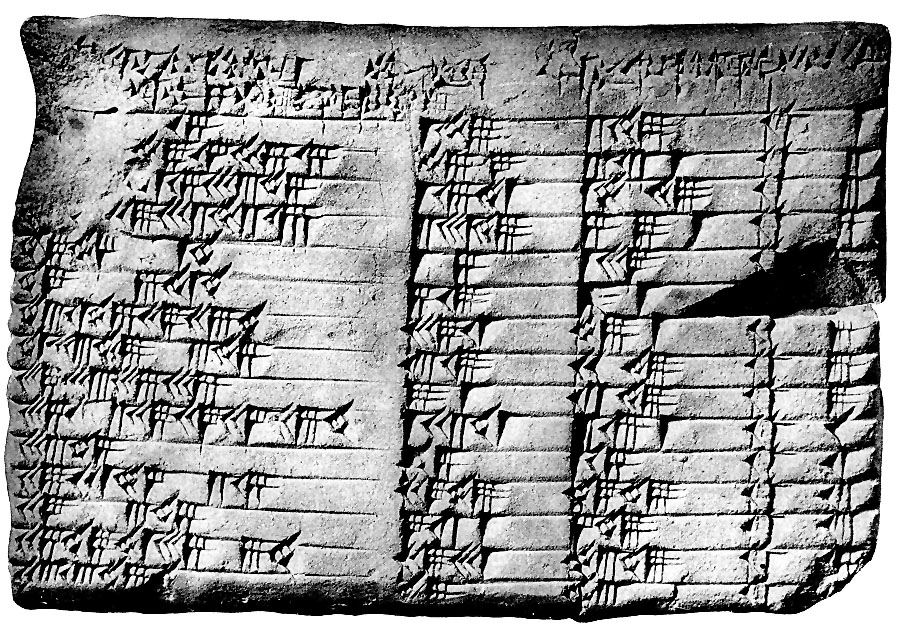
\includegraphics[width=10cm]{pic/Plimpton_322.jpg}
  \end{center}

  \caption{La tablilla babilónica Plimpton 322 (cerca de 1800 a. C.) que enumera
    algunas ternas pitagóricas. Véase \cite[\S I.V]{Weil-history}}
\end{figure}

Las ternas pitagóricas corresponden a los enteros de Gauss cuya norma es un
cuadrado: $N (x+yi) = z^2$. Puesto que $N (\alpha^2) = N (\alpha)^2$, podemos
generar las ternas pitagóricas tomando cuadrados de los enteros de Gauss.
Por ejemplo,
\[ (2 + i)^2 = 3 + 4i, \quad
   (3 + 2i)^2 = 5 + 12i, \quad
   (4 + 3i)^2 = 7 + 24i. \]

En general, tenemos $(a + bi)^2 = a^2 - b^2 + 2ab i$, así que para cualesquiera
$a,b \in \ZZ$ se obtiene una terna pitagórica
\begin{equation}
  \label{eqn:cuadrado-de-entero-de-gauss}
  (a^2 - b^2, \, 2ab, \, a^2 + b^2).
\end{equation}

Nuestro objetivo es probar que esencialmente todas las ternas pitagóricas surgen
de esta manera.

Notamos que si $(x,y,z)$ es una terna pitagórica, entonces $(cx, cy, cz)$
también lo es para cualquier $c \in \ZZ$. Por este motivo será conveniente
considerar solamente las ternas \textbf{primitivas} que satisfacen
$\gcd (x,y,z) = 1$ (lo que también equivale a $\gcd (x,y) = 1$). Las ternas
primitivas corresponden a los puntos \emph{racionales} en el círculo unitario
$x^2 + y^2 = 1$, como por ejemplo
\[ \Bigl(\frac{3}{5}, \frac{4}{5}\Bigr), ~
   \Bigl(\frac{5}{13}, \frac{12}{13}\Bigr), ~
   \Bigl(\frac{7}{25}, \frac{24}{25}\Bigr). \]

Si $(x,y,z)$ es una terna primitiva, se ve que $x$ e $y$ no pueden ser impares
al mismo tiempo. Efectivamente, en el caso contrario $x^2 + y^2 \equiv 1 + 1 = 2
\pmod{4}$, pero los cuadrados módulo $4$ son $0$ y $1$. Entonces, sin pérdida de
generalidad (intercambiando $x$ e $y$ si necesario), se puede suponer que $x$ es
impar e $y$ es par, de acuerdo con la expresión
\eqref{eqn:cuadrado-de-entero-de-gauss}.

\begin{teorema}
  Sea $(x,y,z)$ una terna pitagórica primitiva, donde $x$ es impar e $y$ es
  par. Luego, existen enteros coprimos $a > b > 0$ tales que
  $$x = a^2 - b^2, \quad y = 2ab, \quad z = a^2 + b^2.$$

  \begin{proof}
    Consideremos el entero de Gauss $x + yi$. Por nuestra hipótesis,
    $$N (x + yi) = (x + yi)\,(x - yi) = z^2.$$

    No es difícil ver que si $x$ e $y$ son coprimos y tienen diferente paridad,
    entonces $\gcd (x + yi, \, x - yi) = 1$ (ejercicio). Usando esto y el hecho
    de que su producto es un cuadrado,
    \emph{gracias a la factorización única en $\ZZ [i]$} podemos concluir que
    $x \pm yi$ son también cuadrados; existen $\alpha = a + bi \in \ZZ[i]$ y
    $u \in \ZZ[i]^\times$ tales que
    $$x+yi = u\alpha^2 = u\,(a^2 - b^2 + 2ab i).$$
    Dado que $-1 = i^2$, podemos asumir que $u \in \{ +1, +i \}$. Nuestra
    hipótesis de que $x$ es impar e $y$ es par implica que $u = +1$. Además,
    $x,y > 0$, así que $a > b > 0$. En fin, $\gcd (x,y) = 1$ implica que
    $\gcd (a,b) = 1$.
  \end{proof}
\end{teorema}

Nuestra demostración usa de manera esencial la factorización única en
$\ZZ [i]$. A saber, usamos que si $\alpha\beta = \gamma^2$ para
$\gcd (\alpha,\beta) = 1$, entonces $\alpha \sim \alpha'^2$ y
$\beta \sim \beta'^2$ para algunos $\alpha', \beta'$. Sin factorización
única no se puede llegar a esta conclusión.

\begin{ejemplo}
  Consideremos el anillo $\ZZ [\sqrt{-5}]$. En este caso las unidades son
  $\ZZ [\sqrt{-5}]^\times = \{ \pm 1 \}$. Los números
  $$\alpha = 2 + 3\sqrt{-5}, \quad \overline{\alpha} = 2 - 3\sqrt{-5}$$
  tienen norma
  $$N (\alpha) = \alpha\overline{\alpha} = 7^2.$$
  Dado que $a^2 + 5b^2 \ne 7$ para ningún $a,b \in \ZZ$,
  se ve que $\alpha$ y $\overline{\alpha}$ son irreducibles, no asociados entre
  sí. Su producto es un cuadrado, pero no son asociados con cuadrados
  (¡son irreducibles!). Aquí no hay ninguna contradicción porque
  $\ZZ [\sqrt{-5}]$ no es un dominio de factorización única.
\end{ejemplo}

%%%%%%%%%%%%%%%%%%%%%%%%%%%%%%%%%%%%%%%%%%%%%%%%%%%%%%%%%%%%%%%%%%%%%%%%%%%%%%%%

\section{Ecuación de Fermat \texorpdfstring{$x^3 + y^3 = z^3$}{$x³ + y³ = z³$}}

El lector probablemente ha escuchado del \textbf{último teorema de Fermat} que
afirma que para $n \ge 3$ la ecuación $x^n + y^n = z^n$ no tiene soluciones
enteras con $xyz \ne 0$. La prueba de este resultado (concluida por Andrew Wiles
en 1995) fue uno de los logros más publicitados de las matemáticas del siglo
pasado.

El caso particular de $n = 3$ fue resuelto por Euler. Aquí vamos a ver una
demostración con los enteros de Eisenstein $\ZZ [\zeta_3]$. Curiosamente,
el mismo Euler trabajaba con el anillo más pequeño
$\ZZ [\sqrt{-3}] \subsetneq \ZZ [\zeta_3]$, suponiendo erróneamente que este
tiene factorización única. (Véase \cite[Chapter 2]{Edwards-1996} para más
detalles.)

Antes de lanzarnos en la prueba, notamos que con las terceras raíces de la
unidad la ecuación de Fermat se factoriza como
$$x^3 + y^3 = (x + y)\,(x + \zeta_3 y)\,(x + \zeta_3^2 y) = z^3,$$
y esto explica la utilidad de los enteros de Eisenstein en nuestro problema.

\vspace{1em}

\marginpar{\small Lectura\\adicional}

Para el resto de esta sección fijemos el primo de Eisenstein
$\pi = 1 - \zeta_3$. Recordemos que $\ZZ [\zeta_3]/(\pi) \cong \FF_3$.

\begin{lema}
  \label{lema:FLT-3-1}
  La ecuación $x^3 + y^3 = uz^3$, donde $u \in \ZZ [\zeta_3]^\times$, no tiene
  soluciones $x,y,z \in \ZZ [\zeta_3]$ con $\pi \nmid xyz$.

  \begin{proof}
    Primero notamos que si $\pi \nmid x$, entonces $x \equiv \pm 1 \pmod{\pi}$,
    lo cual implica que $x^3 \equiv \pm 1 \pmod{\pi^4}$. Por ejemplo,
    si $x \equiv 1 \pmod{\pi}$, podemos escribir $x = 1 + \pi t$ para
    $t \in \ZZ [\zeta_3]$ y factorizar
    \[ x^3 - 1 = (x - 1)\,(x - \zeta_3)\,(x - \zeta_3^2)
           = \cdots = \pi^3 \, t \, (t + 1) \, (t - \zeta_3^2). \]
    Aquí $\zeta_3^2 \equiv 1 \pmod{\pi}$, y para cualquier residuo
    $t \equiv 0, +1, -1 \pmod{\pi}$ se ve que $x^3 - 1 \equiv 0 \pmod{\pi^4}$.

    Ahora bien, si $x^3 + y^3 = uz^3$ y $\pi \nmid xyz$, entonces
    $$\pm 1 \pm 1 \equiv \pm u \pmod{\pi^4}.$$
    Es fácil verificar que todas las opciones para los signos $\pm$ y
    $u \in \ZZ [\zeta_3]^\times$ nos llevan a una contradicción (note que
    $\pi^4 \sim 9$, así que se trata de los restos módulo $9$ en $\ZZ
    [\zeta_3]$).
  \end{proof}
\end{lema}

\begin{lema}
  \label{lema:FLT-3-2}
  Si $x^3 + y^3 = uz^3$ para $x,y,z \in \ZZ [\zeta_3]$ y
  $u \in \ZZ [\zeta_3]^\times$, y $\pi \nmid xy$, $\pi \mid z$, entonces
  $\pi^2 \mid z$.

  \begin{proof}
    Como en la prueba del lema anterior, se obtiene
    $$\pm 1 \pm 1 \equiv uz^3 \pmod{\pi^4}.$$
    Si $uz^3 \equiv \pm 2 \pmod{\pi^4}$, entonces $\pi \mid 2$, lo cual no es
    cierto. Por otra parte, si $uz^3 \equiv 0 \pmod{\pi^4}$, entonces
    $$3 v_\pi (z) = v_\pi (z^3) \ge 4,$$
    lo que implica $v_\pi (z) \ge 2$.
  \end{proof}
\end{lema}

La idea clave, que el mismo Fermat aplicó al caso de $n = 4$ el método del
descenso infinito, que en nuestro caso está contenido en el siguiente lema.

\begin{lema}[Descenso]
  \label{lema:FLT-3-3}
  Supongamos que $x^3 + y^3 = uz^3$, para $x,y,z\in \ZZ[\zeta_3]$ y
  $u \in \ZZ [\zeta_3]^\times$, donde $\gcd (x,y) = 1$, $\pi \nmid xy$,
  $v_\pi (z) \ge 2$. Entonces, existen $x_1, y_1, z_1 \in \ZZ [\zeta_3]$
  y $\epsilon \in \ZZ [\zeta_3]^\times$ tales que
  $$x_1^3 + y_1^3 = \epsilon z_1^3,$$
  y $\pi \nmid x_1 y_1$, $v_\pi (z_1) = v_\pi (z) - 1$.

  \begin{proof}
    Como hemos observado, la ecuación se factoriza como
    $$(x + y) \, (x + \zeta_3 y) \, (x + \zeta_3^2 y) = uz^3.$$
    Dado que por nuestra hipótesis
    $$v_\pi (uz^3) = 3 v_\pi (z) \ge 6,$$
    por lo menos uno de los tres factores debe ser divisible por
    $\pi^2$. Remplazando $y$ con $\zeta_3 y$ o $\zeta_3^2 y$, podemos asumir que
    $\pi^2 \mid (x + y)$. Ahora

    \begin{equation}
      \label{eqn:valuacion-x+zeta-y}
      v_\pi (x + \zeta_3 y) = v_\pi (x + y - (1 - \zeta_3) y)
          = \min \{ v_\pi (x+y), v_\pi (\pi y) \} = 1.
    \end{equation}
    De la misma manera,
    \begin{equation}
      \label{eqn:valuacion-x+zeta2-y}
      v_\pi (x + \zeta_3^2 y) = 1.
    \end{equation}
    Entonces,
    \begin{equation}
      \label{eqn:valuacion-x+y}
      v_\pi (x+y) = 3 v_\pi (z) - 2.
    \end{equation}

    Tenemos
    \begin{equation}
      \label{eqn:mcd-tres-factores-x3+y3}
      \gcd (x + y, x + \zeta_3 y) = \gcd (x + y, x + \zeta_3^2 y)
          = \gcd (x + \zeta_3 y, x + \zeta_3^2 y) = \pi.
    \end{equation}
    Por ejemplo, sea $\rho$ un primo tal que $\rho \not\sim \pi$ y
    $\rho \mid (x+y)$ y $\rho \mid (x + \zeta_3 y)$. Entonces,
    $\rho \mid (1 - \zeta_3) y = \pi y$ e $\rho \mid y$. Esto también implicaría
    que $\rho \mid x$, pero $\gcd (x,y) = 1$ por nuestra hipótesis. Entonces,
    el único primo que divide a $x + y$ e $x + \zeta_3 y$ es $\pi$.

    Usando \eqref{eqn:valuacion-x+zeta-y}, \eqref{eqn:valuacion-x+zeta2-y},
    \eqref{eqn:valuacion-x+y}, \eqref{eqn:mcd-tres-factores-x3+y3} podemos
    escribir
    \begin{align*}
      \tag{a} x + y & = u_1 \alpha^3 \pi^{3 v_\pi (z) - 2},\\
      \tag{b} x + \zeta_3 y & = u_2 \beta^3 \pi,\\
      \tag{c} x + \zeta_3^2 y & = u_2 \beta^3 \pi,
    \end{align*}
    donde $\pi \nmid \alpha\beta\gamma$, $u_1,u_2,u_3 \in \ZZ [\zeta_3]^\times$ y
    $$\gcd (\alpha,\beta) = \gcd (\alpha,\gamma) = \gcd (\beta,\gamma) = 1.$$

    La ecuación $\mathrm{(a)} + \zeta_3 \mathrm{(b)} + \zeta_3^2 \mathrm{(c)}$
    nos da
    \[ (\underbrace{1 + \zeta_3 + \zeta_3^2}_{=0})\,(x + y)
           = u_1 \alpha^3 \pi^{3 v_\pi (z) - 2}
                 + \zeta_3 u_2 \beta^3 \pi
                 + \zeta_3^2 u_2 \beta^3 \pi. \]
    Al cancelar $\pi$, nos queda
    \[ \zeta_3 u_2 \beta^3 + \zeta_3^2 u_2 \beta^3
           = -u_1 \alpha^3 \pi^{3 (v_\pi (z) - 1)}. \]
    Pongamos
    $$x_1 = \beta, \quad y_1 = \gamma, \quad z_1 = \alpha \pi^{v_\pi (z) - 1}.$$
    Entonces, para ciertas unidades
    $\epsilon_1, \epsilon_2 \in \ZZ[\zeta_3]^\times$ se cumple
    $$x_1^3 + \epsilon_1 y_1^3 = \epsilon_2 z_1^3.$$
    Tenemos
    $$v_\pi (z_1^3) = 3 v_\pi (z) - 3 > 2,$$
    así que la reducción módulo $\pi^2$ nos da
    $$\pm 1 \pm \epsilon_1 \equiv 0 \pmod{\pi^2}.$$
    Analizando todas las posibilidades para
    $\epsilon_1 \in \ZZ [\zeta_3]^\times$ notamos que la única posibilidad es
    $\epsilon_1 = \mp 1$. Remplazando $y$ por $-y$ si necesario, llegamos a la
    ecuación de la forma
    $$x_1^3 + y_1^3 = \epsilon z_1^3,$$
    donde $\epsilon \in \ZZ [\zeta_3]^\times$, $\pi \nmid x_1 y_1$,
    $v_\pi (z_1) = v_\pi (z) - 1$.
\end{proof}
\end{lema}

Notamos que los argumentos de arriba usan la factorización única en
$\ZZ [\zeta_3]$. Ahora estamos listos para probar el último teorema de Fermat
para $n = 3$. Ya que hemos trabajado con el anillo $\ZZ [\zeta_3]$,
el resultado será un poco más general.

\begin{teorema}
  La ecuación $x^3 + y^3 = uz^3$ para $u \in \ZZ [\zeta_3]^\times$ no tiene
  soluciones $x,y,z \in \ZZ [\zeta_3]$ con $xyz \ne 0$.

  \begin{proof}
    Asumamos que $x^3 + y^3 = uz^3$. El lema~\ref{lema:FLT-3-1} dice que
    necesariamente $\pi \mid xyz$.

    Supongamos que se cumple $\pi \nmid xy$ e $\pi \mid z$. Consideremos la
    solución con el valor de $v_\pi (z)$ más pequeño posible (entre todas las
    posibilidades para $u \in \ZZ [\zeta_3]^\times$). En este caso los
    lemas~\ref{lema:FLT-3-2} y \ref{lema:FLT-3-3} nos llevan a una
    contradicción.

    En fin, supongamos que $\pi \mid x$ y $\pi \nmid yz$. En este caso
    $u \equiv \pm 1 \pmod{\pi^3}$. Sin embargo, esto implica que $u = \pm 1$ y
    la ecuación puede ser escrita como $(\mp z)^3 + (-y)^3 = x^3$, lo cual
    corresponde al caso anterior.
  \end{proof}
\end{teorema}

\begin{comentario}
  De manera parecida, el se puede probar que $x^4 + y^4 = z^4$ no tiene
  soluciones no triviales, usando los enteros de Gauss $\ZZ [i]$. De hecho, el
  argumento demostraría el resultado para $x,y,z\in \ZZ [i]$. En este caso hay
  que considerar el primo $\pi = 1 + i$ (note que $\pi^2 \sim 2$). Para los
  detalles, véase por ejemplo \cite[\S I.3]{Ribenboim-FLT}.

  Estas pruebas usan la factorización única en los anillos ciclotómicos
  $\ZZ [\zeta_3]$ y $\ZZ [i] = \ZZ [\zeta_4]$. En general, $\ZZ [\zeta_n]$
  no tiene factorización única. Curiosamente, esto falla por primera vez para
  $n = 23$.

  Los métodos mencionados establecen algunos casos particulares del último
  teorema de Fermat para anillos de números más grandes que $\ZZ$. Sin embargo,
  el caso general de $n \ge 3$ es un problema abierto: no se sabe si la ecuación
  de Fermat $x^n + y^n = z^n$ no tiene soluciones no triviales en $\ZZ [i]$,
  $\ZZ [\zeta_3]$, etc.\footnote{Véase por ejemplo
    \url{https://mathoverflow.net/questions/90972/} y \cite{Turcas-2018}
    para el reciente progreso.}
\end{comentario}

%%%%%%%%%%%%%%%%%%%%%%%%%%%%%%%%%%%%%%%%%%%%%%%%%%%%%%%%%%%%%%%%%%%%%%%%%%%%%%%%

\section{Puntos enteros en curvas \texorpdfstring{$y^2 = x^3 + t$}{y² = x³ + t}}

Consideremos la curva plana definida por la ecuación
$$E\colon y^2 = x^3 - 1.$$

\begin{figure}
  \begin{center}
    \includegraphics{pic/y2-x3-1.pdf}
  \end{center}

  \caption{Curva elíptica $y^2 = x^3 - 1$}
  \label{fig:y2-x3-1}
\end{figure}

Un famoso teorema de Siegel nos dice que el conjunto de los puntos enteros sobre
cualquier curva elíptica
$$E\colon x^3 + ax + b, \quad a, b \in \ZZ, ~ 4a^3 + 27 b^2 \ne 0$$
es siempre finito \cite[\S X.3]{Silverman-GTM106}. En este caso particular,
una búsqueda sugiere que la única solución es $(1,0)$, pero ¿cómo probarlo?

\begin{proposicion}
  La ecuación $y^2 = x^3 - 1$ tiene única solución entera $(x,y) = (1,0)$.

  \begin{proof}
    Supongamos que $x,y\in \ZZ$ cumplen $y^2 = x^3 - 1$. Primero notamos que
    $x^3 - 1 \not\equiv 1 \pmod{4}$, así que $y$ debe ser par. En el anillo
    $\ZZ [i]$ podemos factorizar nuestra expresión como
    $$x^3 = (y+i)\,(y-i).$$
    Dejo como un ejercicio comprobar que para $y$ par se tiene
    $\gcd (y+i,y-i) = 1$. Luego, puesto que $y+i$ e $y-i$ son coprimos y su
    producto es un cubo, se cumple
    $$y + i = u\,(a + bi)^3,$$
    para algunos $u \in \ZZ [i]^\times$, $a,b \in \ZZ$. Todo elemento de
    $\ZZ [i]^\times = \{ \pm 1, \pm i \}$ es un cubo, así que sin pérdida de
    generalidad $u = 1$. Tenemos
    $$y + i = (a + bi)^3 = a\,(a^2 - 3b^2) + b\,(3a^2 - b^2)\,i.$$
    De $1 = b\,(3a^2 - b^2)$ se ve que la única solución posible es
    $a = 0, b = -1$. Esto nos permite concluir que $y = 0$, y luego $x = 1$.
  \end{proof}
\end{proposicion}

Ahora consideremos la ecuación parecida
$$y^2 = x^3 - 19.$$
Podemos tratar de aplicar el mismo truco y factorizar en
el anillo $\ZZ [\sqrt{-19}]$
$$x^3 = (y + \sqrt{-19})\,(y - \sqrt{-19}).$$

Notamos que $x^3 - 19 \not\equiv 1 \pmod{8}$, mientras que
$y^2 \equiv 1 \pmod{8}$ si $y$ es impar. Entonces, $y$ es necesariamente par,
y además se ve que $y \ne 0$. En este caso
$\gcd (y + \sqrt{-19}, y - \sqrt{-19}) = 1$, en el sentido que
$$(y + \sqrt{-19}, y - \sqrt{-19}) = \ZZ [\sqrt{-19}].$$
(¡Ejercicio!) Como antes, podemos escribir
\[ y + \sqrt{-19} = (a + b\sqrt{-19})^3
       = a\,(a^2 - 57b^2) + b\,(3a^2 - 19b^2)\,\sqrt{-19}. \]
(Note que $\ZZ [\sqrt{-19}]^\times = \{ \pm 1 \}$, así que podemos olvidar de la
unidad.) En particular, $b\,(3a^2 - 19b^2) = 1$, pero esta ecuación no tiene
soluciones enteras. Entonces, parece que la ecuación $y^2 = x^3 - 19$ no tiene
soluciones enteras\dots{} Sin embargo, no es difícil verificar que
$$7^3 - 19 = 324 = 18^2,$$
así que $(7, \pm 18)$ es una solución entera. Entonces, nuestra lógica nos
falló en algún momento.

\vspace{1em}

El problema es que el anillo $\ZZ [\sqrt{-19}]$, a diferencia de $\ZZ [i]$,
no tiene factorización única (véanse los ejercicios para una prueba).
Con las herramientas que vamos a desarrollar en nuestro curso, veremos que
el anillo más grande $\ZZ \Bigl[\frac{1+\sqrt{-19}}{2}\Bigr]$ sí tiene
factorización única, así que hay que trabajar en este anillo.

\begin{proposicion}
  Las únicas soluciones enteras de la ecuación $y^2 = x^3 - 19$ son
  $(x,y) = (7, \pm 18)$.

  \begin{proof}
    Denotemos $\alpha = \frac{1+\sqrt{-19}}{2}$. Notamos que
    $\alpha^2 - \alpha + 5 = 0$. Como mencionamos, $\ZZ [\alpha]$ tiene
    factorización única. Tenemos $\ZZ [\alpha]^\times = \{ \pm 1 \}$.
    El argumento de arriba nos da
    \[ (y-1) + 2\alpha = y + \sqrt{-19} = \left(a + b\alpha\right)^3
           = (a^3 - 15ab^2 - 5b^3) + (3a^2 + 3ab - 4b^2)\,b \alpha. \]
    La ecuación $(3a^2 + 3ab - 4b^2)\,b = 2$ implica que $b = \pm 1$, $\pm 2$,
    y se ve que las únicas soluciones enteras son
    $$(a,b) = (-2,1), (1,1).$$
    Sustituyendo estos valores, llegamos precisamente a $y = \pm 18$, y luego
    $x^3 = 18^2 + 19 = 343$, así que $x = 7$.
  \end{proof}
\end{proposicion}

\begin{figure}
  \begin{center}
    \includegraphics{pic/y2-x3-19.pdf}
  \end{center}

  \caption{Curva elíptica $y^2 = x^3 - 19$}
  \label{fig:y2-x3-19}
\end{figure}

\begin{ejemplo}
  He aquí los puntos enteros sobre algunas curvas de la forma $y^2 = x^3 + t$.
  Para la teoría detrás de esta ecuación diofántica, véase por ejemplo
  \cite{Cohen-GTM239}.

  \begin{center}
    \begin{tabular}{ll|ll}
      $y^2 = x^2 + 1\colon$ & $(-1,0), (0,\pm 1), (2,\pm 3)$ & $y^2 = x^3 - 1\colon$ & $(1,0)$ \\
      $y^2 = x^2 + 2\colon$ & $(-1,\pm 1)$ & $y^2 = x^3 - 2\colon$ & $(3,\pm 5)$ \\
      $y^2 = x^2 + 3\colon$ & $(1,\pm 2)$ & $y^2 = x^2 - 3\colon$ & --- \\
      $y^2 = x^2 + 4\colon$ & $(0,\pm 2)$ & $y^2 = x^2 - 4\colon$ & $(2,\pm 2), (5,\pm 11)$ \\
      $y^2 = x^2 + 5\colon$ & $(-1,\pm 2)$ & $y^2 = x^2 - 5\colon$ & --- \\
      $y^2 = x^2 + 6\colon$ & --- & $y^2 = x^2 - 6\colon$ & --- \\
      $y^2 = x^2 + 7\colon$ & --- & $y^2 = x^2 - 7\colon$ & $(2,\pm 1), (32,\pm 181)$ \\
      $y^2 = x^2 + 8\colon$ & $(-2,0), (1,\pm 3), (2,\pm 4), (46,\pm 312)$ & $y^2 = x^2 - 8\colon$ & $(2,0)$ \\
      $y^2 = x^2 + 9\colon$ & $(-2,\pm 1), (0,\pm 3), (3,\pm 6), (6,\pm 15), (40,\pm 253)$ & $y^2 = x^2 - 9\colon$ & --- \\
      $y^2 = x^2 + 10\colon$ & $(-1,\pm 3)$ & $y^2 = x^2 - 10\colon$ & --- \\
    \end{tabular}
  \end{center}
\end{ejemplo}

%%%%%%%%%%%%%%%%%%%%%%%%%%%%%%%%%%%%%%%%%%%%%%%%%%%%%%%%%%%%%%%%%%%%%%%%%%%%%%%%

\section{Ecuación de Pell \texorpdfstring{$x^2 - dy^2 = 1$}{x² - dy² = 1}}

Sea $d > 0$ un entero libre de cuadrados. La ecuación diofántica
$$x^2 - dy^2 = 1$$
se conoce como la \textbf{ecuación de Pell}\footnote{John Pell (1611--1685),
  matemático inglés. No hay documentos que demuestren que Pell trabajó en algún
  momento de su vida en la «ecuación de Pell»; la atribución errónea del
  nombre se debe a Euler. Así que como matemático, Pell es conocido por una
  ecuación que nunca estudió.}.
Nuestro objetivo es describir las soluciones enteras.

Por ejemplo, consideremos la ecuación $x^2 - 3y^2 = 1$ (véase la figura
\ref{fig:pell-3}). Algunas soluciones evidentes son
$$(1, 0), ~ (2, 1), ~ (7, 4).$$
Podemos usar PARI/GP para encontrar más soluciones. Basta fijarnos, por ejemplo,
en los valores de $y$, y luego $x = \pm\sqrt{1 + 3y^2}$.

\begin{figure}
  \begin{center}
    \includegraphics{pic/pell-3.pdf}
  \end{center}

  \caption{Algunos puntos enteros en la curva $x^2 - 3y^2 = 1$}
  \label{fig:pell-3}
\end{figure}

\begin{shaded}
\begin{verbatim}
? pell_sol_naive (d,n) = {
  for (y=0,n,
    if (issquare (1+d*y^2),
      print ([sqrtint (1+d*y^2), y])
    )
  )
};

? pell_sol_naive (3,10^6)
[1, 0]
[2, 1]
[7, 4]
[26, 15]
[97, 56]
[362, 209]
[1351, 780]
[5042, 2911]
[18817, 10864]
[70226, 40545]
[262087, 151316]
[978122, 564719]
\end{verbatim}
\end{shaded}

Consideremos el anillo $\ZZ [\sqrt{3}]$. Este viene con la norma
$$N (x + y\sqrt{3}) = (x + y\sqrt{3})\,(x - y\sqrt{3}) = x^2 - 3y^2,$$
y el argumento que ya hemos visto arriba demuestra que
\[ \ZZ [\sqrt{3}]^\times
       = \{ \alpha \in \ZZ [\zeta_3] \mid N (\alpha) = \pm 1 \}. \]
Considerando $x^2 - 3y^2$ módulo $4$, notamos que la norma $-1$ nunca
ocurre. Entonces, las soluciones de ${x^2 - 3y^2 = 1}$ corresponden exactamente
a las unidades $u \in \ZZ [\sqrt{3}]^\times$. Por ejemplo, la solución $(2,1)$
corresponde a la unidad $u = 2 + \sqrt{3}$, y nuestra sucesión de arriba nada
más viene de las potencias $u^n$ para $n = 0,1,2,3,\ldots$ Por ejemplo,
\begin{align*}
  (2 + \sqrt{3})^2 & = 7 + 4\sqrt{3},\\
  (2 + \sqrt{3})^3 & = 26 + 15\sqrt{3}.
\end{align*}

\begin{shaded}
\begin{verbatim}
? K = nfinit(x^2-3);
? u = 2+x;
? for (n=1,10, u=nfeltmul(K,u,2+x); print(u));
[7, 4]~
[26, 15]~
[97, 56]~
[362, 209]~
[1351, 780]~
[5042, 2911]~
[18817, 10864]~
[70226, 40545]~
[262087, 151316]~
[978122, 564719]~
\end{verbatim}
\end{shaded}

En particular, notamos que $u^m \ne u^n$ para $m \ne n$, así que la ecuación
tiene un número infinito de soluciones. De hecho, en el caso contrario
$u^{m-n} = 1$, pero los elementos de $\ZZ [\sqrt{3}]$ son números reales,
y las únicas raíces de la unidad en $\RR$ son $\pm 1$.

El número $2 + \sqrt{3}$ se llama la \textbf{unidad fundamental} y surge de la
siguiente manera.

\begin{lema}
  \label{lema:unidad-fundamental-3}
  El número $2 + \sqrt{3}$ es la unidad más pequeña
  $u \in \ZZ [\sqrt{3}]^\times$ que cumple $u > 1$.

  \begin{proof}
    Supongamos que existe una unidad $u = a + b\sqrt{3}$ que cumple
    $$1 \le u \le 2 + \sqrt{3}.$$
    Luego, $u^{-1} = a - b\sqrt{3}$, y tomando los inversos se obtiene la
    desigualdad
    $$2 - \sqrt{3} \le u^{-1} \le 1.$$
    Sumando las dos desigualdades, llegamos a
    $$1 < 3 - \sqrt{3} \le u + u^{-1} \le 3 + \sqrt{3} < 5.$$
    El número $u + u^{-1} = 2a$ es par, así que hay solo dos posibilidades:
    $$u + u^{-1} = 2 \quad\text{o}\quad u + u^{-1} = 4.$$

    La primera ecuación implica que $u = 1$, mientras que la segunda implica que
    $u = 2 + \sqrt{3}$.
\end{proof}
\end{lema}

\begin{teorema}
  Toda unidad $u \in \ZZ [\sqrt{3}]^\times$ es de la forma $\pm (2 +
  \sqrt{3})^n$ para algún $n \in \ZZ$. En otras palabras, hay isomorfismo de
  grupos
  \[ \ZZ [\sqrt{3}]^\times
       \cong \langle \pm 1\rangle \times \langle 2 + \sqrt{3}\rangle
       \cong \ZZ/2\ZZ \oplus \ZZ. \]
\end{teorema}

Este es un caso muy particular del \textbf{teorema de unidades de Dirichlet} que
será uno de los resultados más importantes del curso.

\begin{proof}
  Está claro que $\pm (2 + \sqrt{3})^n$ son unidades, hay que probar que no hay
  otras. Sea $u \in \ZZ [\sqrt{3}]^\times$ una unidad. Pasando a $u^{-1}$ y
  cambiando el signo, podemos asegurarnos de que $u \ge 1$. En este caso habrá
  algún $n = 0,1,2,3,\ldots$ tal que
  $$(2 + \sqrt{3})^n \le u < (2 + \sqrt{3})^{n+1}.$$
  Luego,
  $$1 \le u\,(2 + \sqrt{3})^{-n} < 2 + \sqrt{3},$$
  y el lema de arriba implica que $u = (2 + \sqrt{3})^n$.
\end{proof}

Ahora consideremos la ecuación $x^2 - 2011 y^2 = 1$. Empleando la búsqueda tonta
para todo $y \le N$ (como por ejemplo al inicio de esta sección), no se
encuentra ninguna solución no trivial.

\begin{shaded}
\begin{verbatim}
? #
   timer = 1 (on)
? pell_sol_naive (2011,10^7)
[1, 0]
time = 5,093 ms.
? pell_sol_naive (2011,10^8)
[1, 0]
time = 50,371 ms.
\end{verbatim}
\end{shaded}

¿Será que para $d = 2011$ la ecuación de Pell ya no tiene soluciones no
triviales por alguna razón? De hecho no, $2011$ no tiene nada de especial,
solo que en este caso la unidad fundamental es

\begin{multline*}
  22903355954053525066202335319378237605968890\\
  + 510732021116138713675018566232201605320997\,\sqrt{2011}.
\end{multline*}
Ninguna búsqueda razonable puede llegar a estos números.

\begin{shaded}
  Para calcular la unidad fundamental en un campo cuadrático real, podemos hacer
  lo siguiente.
\begin{verbatim}
? quadunit(4*3)
% = 2 + w
? quadunit(4*2011)
% = 22903355954053525066202335319378237605968890
        + 510732021116138713675018566232201605320997*w
? norm (%)
% = 1
\end{verbatim}
  Hemos escrito \texttt{quadunit(4*2011)} porque $d = 2011 \equiv 2,3 \pmod{4}$,
  y el campo $\QQ (\sqrt{2011})$ tiene discriminante $4\cdot 2011$; esto será
  explicado más adelante en el curso. Además, notamos que si
  $d \equiv 1 \pmod{4}$, entonces \texttt{quadunit($d$)} devuelve la unidad
  fundamental en el anillo $\ZZ \Bigl[\frac{1+\sqrt{d}}{2}\Bigr]$.
\end{shaded}

Salvo algunos detalles, la ecuación de Pell siempre se resuelve encontrando
la unidad fundamental correspondiente. Más adelante en el curso veremos un
algoritmo para encontrarla.

\begin{ejemplo}
  He aquí una breve lista de unidades fundamentales (es decir, las unidades más
  pequeñas tales que $u > 1$) en los anillos de la forma $\ZZ [\sqrt{d}]$
  (y $\ZZ \Bigl[\frac{1+\sqrt{d}}{2}\Bigr]$ para $d \equiv 1 \pmod{4}$).

  \renewcommand{\arraystretch}{1.5}
  \begin{center}
    \begin{tabular}{rcccccccc}
      \hline
      $R\colon $ & $\ZZ [\sqrt{2}]$ & $\ZZ [\sqrt{3}]$ & $\ZZ [\sqrt{5}]$ & $\ZZ [\sqrt{6}]$ & $\ZZ [\sqrt{7}]$ & $\ZZ [\sqrt{10}]$ & $\ZZ [\sqrt{11}]$ & $\ZZ [\sqrt{13}]$ \\
      $u\colon$ & $1 + \sqrt{2}$ & $2 + \sqrt{3}$ & $2 + \sqrt{5}$ & $5 + 2\sqrt{6}$ & $8 + 3\sqrt{7}$ & $3 + \sqrt{10}$ & $10 + 3\sqrt{11}$ & $18 + 5\sqrt{13}$ \\
      $N (u)\colon$ & $-1$ & $+1$ & $-1$ & $+1$ & $-1$ & $-1$ & $+1$ & $-1$ \\
      \hline
      $R\colon $ & & & $\ZZ \Bigl[\frac{1+\sqrt{5}}{2}\Bigr]$ & & & & & $\ZZ \Bigl[\frac{1+\sqrt{13}}{2}\Bigr]$ \\
      $u\colon$ & & & $\frac{1+\sqrt{5}}{2}$ & & & & & $1 + \frac{1+\sqrt{13}}{2}$ \\
      $N (u)\colon$ & & & $-1$ & & & & & $-1$ \\
      \hline
    \end{tabular}
  \end{center}
  \renewcommand{\arraystretch}{1}

  Invito al lector a comprobar algunos casos (de la misma manera que hicimos con
  $\ZZ [\sqrt{3}]$ en \ref{lema:unidad-fundamental-3}).
\end{ejemplo}

Para que el lector no piense que los anillos cuadráticos reales $\ZZ [\sqrt{d}]$
tienen algo especial, por ejemplo, tomemos el anillo ciclotómico
$$\ZZ[\zeta_p] \cong \ZZ[x]/(\Phi_p) = \ZZ[x]/(x^{p-1} + x^{p-2} + \cdots + x + 1).$$
Allí la división con resto de polinomios nos da
$$\Phi_p = (x+1)\,(x^{p-2} + x^{p-4} + \cdots + x^3 + x) + 1,$$
lo que demuestra que
\[ (1 + \zeta_p)^{-1} =
   - (\zeta_p + \zeta_p^3 + \cdots + \zeta_p^{p-4} + \zeta_p^{p-1}), \]
así que $1 + \zeta_p \in \ZZ [\zeta_p]^\times$. En general, en el anillo
ciclotómico $\ZZ[\zeta_n]$ habrá muchas unidades, y el grupo
$\ZZ[\zeta_n]^\times$ es finitamente generado de rango $\phi(n)/2 - 1$.
Lo veremos más adelante en el curso.

\pagebreak

\phantomsection

\addcontentsline{toc}{section}{Ejercicios}
\section*{Ejercicios}

\subsection*{Campos y anillos de números}

\begin{ejercicio}[Campos cuadráticos]
  Consideremos una extensión cuadrática $K/\QQ$ (es decir, $[K : \QQ] = 2$).

  \begin{enumerate}
  \item[a)] Demuestre que $K \cong \QQ (\sqrt{d})$ para algún entero libre de
    cuadrados $d$.

  \item[b)] Demuestre que $\QQ (\sqrt{d}) \cong \QQ (\sqrt{d'})$ si y solamente
    si $d = d'$.
  \end{enumerate}

  Advertencia: esto no funciona para el grado mayor que $2$; por ejemplo,
  no todas las extensiones cúbicas son de la forma $\QQ (\sqrt[3]{d})$.
  (¿Puede encontrar algún ejemplo?)
\end{ejercicio}

\begin{ejercicio}
  El \textbf{teorema del elemento primitivo} afirma que para todo campo
  de números $K/\QQ$ existe un elemento $\alpha$ tal que $K = \QQ (\alpha)$.

  \begin{enumerate}
  \item[a)] Revise la prueba estándar en cualquier libro de texto
    \cite[Chapter V, Theorem 4.6]{Lang-Algebra} o
    \cite[Chapter I, Theorem 5.6]{Morandi-GTM167}.

  \item[b)] Encuentre $\alpha$ para
    $K = \QQ (\sqrt{2}, \sqrt{3}, \sqrt{5})$. Exprese
    $\sqrt{2}, \sqrt{3}, \sqrt{5}$ en términos de la base estándar de
    $\QQ (\alpha)$.

  \item[c*)] Use la función \texttt{rnfequation($K$,$f$)} de PARI/GP para
    obtener el polinomio mínimo de $\alpha$.
  \end{enumerate}
\end{ejercicio}

\begin{ejercicio}
  \begin{enumerate}
  \item[a)] Demuestre que los anillos $\QQ$, $\ZZ \Bigl[\frac{1}{n}\Bigr]$,
    $\ZZ_{(p)}$ no son finitamente generados como $\ZZ$-módulos.

  \item[b)] Demuestre que un grupo abeliano $p$-divisible para un primo $p$ no
    puede ser finitamente generado.
  \end{enumerate}
\end{ejercicio}

\begin{ejercicio}
  Sea $f \in \ZZ [x]$ un polinomio mónico irreducible con coeficientes enteros.

  \begin{enumerate}
    \item[a)] Demuestre que el anillo $\ZZ [x] / (f)$ es un $\ZZ$-módulo libre
      de rango $\deg f$ y el campo $\QQ [x] / (f)$ es una extensión de $\QQ$ de
      grado $\deg f$.

    \item[b)] ¿Qué sucede si $f$ no es mónico?
  \end{enumerate}
\end{ejercicio}

\subsection*{Factorización única}

\begin{ejercicio}
  Demuestre que los anillos $\ZZ [x]$ y $k [x,y]$ (donde $k$ es un campo) no son
  dominios de ideales principales. (Son dominios de factorización única, ya que
  para cualquier DFU $R$, el anillo de polinomios $R[X]$ es también un DFU.)
\end{ejercicio}

\begin{ejercicio}
  Demuestre que el anillo de polinomios con un número infinito de variables
  $$k [x_1,x_2,x_3,\ldots] = \bigcup_{n\ge 0} k [x_1,\ldots,x_n]$$
  (unión respecto a las inclusiones naturales) no es noetheriano, pero es un
  dominio de factorización única.

  Este ejemplo explica la condición a) en \ref{thm:caracterizacion-de-DFU} que
  es más débil que la condición noetheriana.
\end{ejercicio}

\begin{ejercicio}
  Demuestre que los siguientes anillos son euclidianos respecto a su norma
  habitual:
  \[ \ZZ [\sqrt{-2}], ~ \ZZ [\sqrt{2}], ~
     \ZZ [\zeta_3] = \ZZ \Bigl[\frac{1+\sqrt{-3}}{2}\Bigr], ~
     \ZZ \Bigl[\frac{1+\sqrt{-7}}{2}\Bigr], ~
     \ZZ \Bigl[\frac{1+\sqrt{-11}}{2}\Bigr]. \]
\end{ejercicio}

\begin{ejercicio}
  En este ejercicio vamos a probar que el anillo
  $R = \ZZ \Bigl[\frac{1+\sqrt{-19}}{2}\Bigr]$ no es euclidiano.

  Supongamos que $R$ es euclidiano (respecto a alguna función
  $\delta\colon R\setminus \{0\} \to \NN$). Sea $\alpha$ un elemento no nulo
  y no invertible con el mínimo posible valor de $\delta (\alpha)$
  (es decir, si $\delta (r) < \delta (\alpha)$, entonces $r = 0$ o
  $r \in R^\times$).

  \begin{enumerate}
  \item[a)] Demuestre que para cualquier $\beta \in R$ se tiene
    $\alpha \mid \beta$, o $\alpha \mid (\beta \pm 1)$.

  \item[b)] Considere qué sucede con $\beta = 2$ y
    $\beta = \frac{1+\sqrt{-19}}{2}$ para concluir que tal $\alpha$ no existe.
  \end{enumerate}

  Más adelante en el curso veremos que $\ZZ \Bigl[\frac{1+\sqrt{-19}}{2}\Bigr]$
  es un dominio de ideales principales. De la misma manera,
  $\ZZ \Bigl[\frac{1+\sqrt{-43}}{2}\Bigr]$,
  $\ZZ \Bigl[\frac{1+\sqrt{-67}}{2}\Bigr]$,
  $\ZZ \Bigl[\frac{1+\sqrt{-163}}{2}\Bigr]$
  son dominios de ideales principales, pero no son euclidianos. La moraleja de
  este ejercicio: la noción de dominio euclidiano no tiene ningún sentido
  profundo; es puramente utilitaria y se ocupa para probar que ciertos anillos
  son dominios de ideales principales. En práctica no es fácil demostrar que
  algo es un dominio euclidiano, ni que no lo es.
\end{ejercicio}

\subsection*{Enteros de Gauss $\ZZ [i]$}

\begin{ejercicio}
  Factorice el número $210$ en $\ZZ [i]$.
\end{ejercicio}

\begin{ejercicio}
  Sean $a,b$ dos enteros coprimos de diferente paridad. Demuestre que
  $\gcd (a + bi, a - bi) = 1$ en $\ZZ [i]$. En particular, si $a$ es par,
  entonces $\gcd (a + i, a - i) = 1$.
\end{ejercicio}

\begin{ejercicio}
  Calcule $\gcd (a + i, a - i)$ y $\gcd (a + 2i, a - 2i)$ en el anillo
  $\ZZ [i]$.

  \emph{Sugerencia: la respuesta depende de $a$ módulo $2$ y $4$.}
\end{ejercicio}

\begin{ejercicio}
  Ya que nuestro curso está dedicado a números algebraicos, hemos usado el
  anillo $\ZZ [i]$ para describir las ternas pitagóricas. He aquí un modo más
  geométrico de hacerlo.

  Notamos que una terna pitagórica primitiva $(x,y,z)$ corresponde a un punto
  racional $(u,v) = \left(\frac{x}{y}, \frac{y}{z}\right)$ en el circulo
  unitario. Fijemos el punto $P = (-1,0)$ y tracemos una recta que pasa por $P$
  y tiene otra intersección $Q$ con el círculo. Esta recta tendrá la ecuación
  $$\ell\colon y = tx + t$$
  para algún $t$.

  \begin{center}
    \includegraphics{pic/circle-parametrization.pdf}
  \end{center}

  La intersección de esta recta con el círculo viene dada por
  $$Q = \left(\frac{1 - t^2}{1 + t^2}, \frac{2t}{1 + t^2}\right).$$ Demuestre
  que de esta manera los puntos racionales en el círculo unitario salvo el punto
  $P$ están en biyección con $t \in \QQ$. Escribiendo $t = \frac{b}{a}$ con
  $\gcd (a,b) = 1$, recupere nuestra parametrización de las ternas pitagóricas
  primitivas.
\end{ejercicio}

\subsection*{Campos y anillos cuadráticos}

\begin{ejercicio}
  Sea $d < 0$ un entero \emph{negativo} libre de cuadrados. Usando la norma
  correspondiente\footnote{En este caso particular,
    $N_{K/\QQ} (\alpha) = \alpha\,\sigma (\alpha)$,
    donde $\Gal (K/\QQ) = \{ 1, \sigma \}$.},
  calcule los grupos de unidades

  \begin{enumerate}
  \item[a)] $\ZZ [\sqrt{d}]^\times$,
  \item[b)] $\ZZ \Bigl[\frac{1+\sqrt{d}}{2}\Bigr]^\times$ para
    $d \equiv 1 \pmod{4}$.
  \end{enumerate}
\end{ejercicio}

\begin{ejercicio}
  Sea $d \ge 3$ un entero libre de cuadrados.

  \begin{enumerate}
    \item[a)] Demuestre que en el anillo $\ZZ [\sqrt{-d}]$ el número $2$ es
      irreducible pero no es primo.

      \emph{Sugerencia: si $d$ es par, $2 \mid (\sqrt{-d})^2$ y si $d$ es impar,
      $2 \mid (1 + \sqrt{-d})\,(1 - \sqrt{-d})$.}

    \item[b)] La misma pregunta para $\ZZ [\sqrt{d}]$ si $d \equiv 1 \pmod{4}$.

      \emph{Sugerencia: $2 \mid (\sqrt{d} + 1)\,(\sqrt{d} - 1)$.}
  \end{enumerate}
\end{ejercicio}

\begin{ejercicio}
  Consideremos el ideal $I = (2, 1 + \sqrt{-3})$ en el anillo $\ZZ [\sqrt{-3}]$.

  \begin{enumerate}
  \item[a)] Demuestre que $I$ no es principal.

    \emph{Sugerencia: use la norma.}

  \item[b)] Demuestre que $I$ es principal en el anillo más grande
    $\ZZ \Bigl[\frac{1+\sqrt{-3}}{2}\Bigr]$.
  \end{enumerate}
\end{ejercicio}

\subsection*{Enteros de Eisenstein $\ZZ [\zeta_3]$}

\begin{ejercicio}
  Factorice el número $210$ en $\ZZ [\zeta_3]$.
\end{ejercicio}

\begin{ejercicio}
  Para un primo $p\equiv 1\pmod{3}$ demuestre que en la expresión
  $4p = u^2 + 27v^2$ los números $u$ y $v$ están bien definidos salvo
  signo.

  \emph{Sugerencia: revise cómo estas expresiones surgen de los enteros de
    Eisenstein $\ZZ [\zeta_3]$ y use la factorización única en $\ZZ [\zeta_3]$.}
\end{ejercicio}

\begin{ejercicio}
  Demuestre que si $\pi\in\ZZ[\zeta_3]$ es un primo de Eisenstein tal que
  $\pi\not\sim 1-\zeta_3$, entonces $1,\zeta_3,\zeta_3^2$ no son congruentes
  módulo $\pi$.
\end{ejercicio}

\begin{ejercicio}
  Sea $\pi \in \ZZ [\zeta_3]$ un primo de Eisenstein tal que
  $N (\pi) = p \equiv 1 \pmod{3}$. Demuestre que entre sus asociados
  $\pi' \sim \pi$ precisamente uno cumple $\pi' \equiv 2 \pmod{3}$.
\end{ejercicio}

\begin{ejercicio}
  Demuestre que $\legendre{\alpha}{\pi}_3 = 1$ si y solamente si $\alpha$ es un
  residuo cúbico en $\ZZ [\zeta_3]/(\pi)$ (es decir, si la congruencia
  $x^3 \equiv \alpha \pmod{\pi}$ tiene solución en $\ZZ [\zeta_3]$).
\end{ejercicio}

\begin{ejercicio}
  Verifique sin computadora si la congruencia
  $$x^3 \equiv 2 - 3\zeta_3 \pmod{23}$$
  tiene solución en $\mathbb{Z} [\zeta_3]$.

  \emph{Sugerencia: en total en $(\mathbb{Z} [\zeta_3]/(23))^\times$ habrá
    $\frac{23^2 - 1}{3} = 177$ cubos y no es una buena idea enumerarlos uno por
    uno\dots}

  En general, dado un primo racional $p \equiv 2 \pmod{3}$, ¿cuándo $2 +
  3\zeta_3$ es un cubo módulo $p$?
\end{ejercicio}

\begin{ejercicio}[\cite{Nagell-1964}]
  Demuestre que la ecuación $x^3 + y^3 = 3z^3$ no tiene soluciones
  $x,y,z \in \ZZ [\zeta_3]$ con $z\ne 0$.
\end{ejercicio}

\subsection*{Ecuación $y^2 = x^3 + t$}

\begin{ejercicio}
  Demuestre que si $a \ne 0$ es par, entonces en el anillo $\ZZ [\sqrt{-19}]$
  $$(a + \sqrt{-19}, a - \sqrt{-19}) = \ZZ [\sqrt{-19}].$$
  (Lo ocupamos en nuestro análisis de la ecuación $y^2 = x^3 - 19$.)
\end{ejercicio}

\begin{ejercicio}
  Encuentre las soluciones enteras de $y^2 = x^3 - 4$.

  \emph{Sugerencia: $y^2 + 4 = (y + 2i)\,(y - 2i)$.}
\end{ejercicio}

\subsection*{Ecuación de Pell y grupos $\ZZ [\sqrt{d}]^\times$ y $\ZZ \Bigl[\frac{\sqrt{d}}{2}\Bigr]^\times$}

\begin{ejercicio}
  Sea $d > 1$ un entero libre de cuadrados. Demuestre que si la ecuación
  $x^2 - dy^2 = -1$ tiene soluciones enteras, entonces $x^2 - dy^2 = +1$
  también tiene soluciones enteras.
\end{ejercicio}

\begin{ejercicio}
  Consideremos la ecuación $x^2 - 3y^2 = n$ para
  $$n = 2,3,4,5,6,7,8,9,10.$$
  ¿Para cuáles de estos $n$ existen soluciones enteras? Demuestre que en este
  caso hay un número infinito de ellas.
\end{ejercicio}

\begin{ejercicio}
  Demuestre que todas las soluciones de la ecuación $x^2 - 3y^2 = 1$ con
  $x,y\ge 0$ enteros vienen dadas por la recurrencia
  \begin{gather*}
    (a_0,b_0) = (1,0), \quad (a_1,b_1) = (2,1),\\
    (a_n,b_n) = 4 (a_{n-1}, b_{n-1}) - (a_{n-2}, b_{n-2}) \text{ para }n\ge 2.
  \end{gather*}
\end{ejercicio}

\begin{ejercicio}
  Describa las soluciones enteras de las ecuaciones
  $$x^2 - dy^2 = +1 \quad\text{y}\quad x^2 - dy^2 = -1,$$
  donde $d = 2$ y $5$.
\end{ejercicio}

\begin{ejercicio}
  Consideremos el anillo $\ZZ \Bigl[\frac{1+\sqrt{5}}{2}\Bigr]$.

  \begin{enumerate}
  \item[a)] Encuentre la unidad más pequeña
    $u \in \ZZ \Bigl[\frac{1+\sqrt{5}}{2}\Bigr]^\times$ tal que $u > 1$.

  \item[b)] Encuentre el índice de subgrupo
    $\Bigl[\ZZ \Bigl[\frac{1+\sqrt{5}}{2}\Bigr]^\times :
           \ZZ [\sqrt{5}]^\times\Bigr]$.
  \end{enumerate}
\end{ejercicio}

\begin{ejercicio}
  Consideremos el anillo ciclotómico $\ZZ [\zeta_5]$.

  \begin{enumerate}
  \item[a)] Demuestre que $u = 1 + \zeta_5$ es una unidad en el anillo 
    y el subgrupo de $\ZZ [\zeta_5]^\times$ generado por $u$ es infinito.

    En realidad,
    $\ZZ [\zeta_5]^\times \cong \mu_{10} (\CC) \times \langle u\rangle$,
    pero lo probaremos más adelante en el curso.

  \item[b)] Demuestre que
    $\ZZ \Bigl[\frac{1 + \sqrt{5}}{2}\Bigr] \subset \ZZ [\zeta_5]$ y calcule
    el índice
    $\Bigl[\ZZ [\zeta_5]^\times :
           \ZZ \Bigl[\frac{1 + \sqrt{5}}{2}\Bigr]^\times \Bigr]$.
  \end{enumerate}
\end{ejercicio}


\chapter{Aritmética de ideales}

La idea de Richard Dedekind consistía en remplazar las operaciones aritméticas
con elementos $\alpha \in R$ por las operaciones con ideales $I\subseteq R$.
Los anillos de números donde este programa funciona sin obstáculos se conocen
como los \textbf{dominios de Dedekind}. Los vamos a definir en este capítulo.

Una gran parte del material de abajo (ideales primos y maximales, localización,
dominios de valuación discreta, etc.) se encuentra en los libros de texto de
álgebra conmutativa. Recomiendo consultar \cite{Atiyah-Macdonald} y
\cite{Reid-UCA}.

\begin{figure}
  \begin{center}
    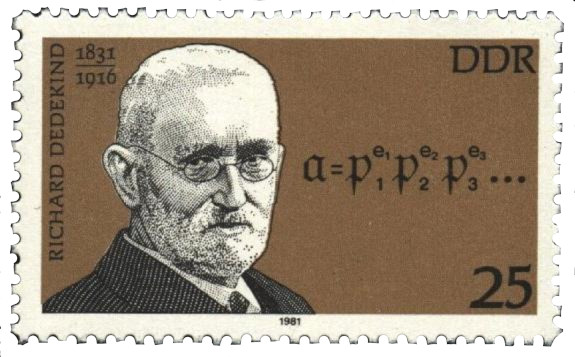
\includegraphics[width=7cm]{pic/Dedekind_stamp.jpg}
  \end{center}

  \caption{Estampilla de la República Democrática Alemana dedicada a Dedekind}
\end{figure}

\pdfbookmark{Clase 5 (24/08/20)}{clase-5}
\section{Operaciones con ideales}
\marginpar{\small Clase 5 \\ 24/08/20}


Sea $R$ un anillo conmutativo. Ya hemos hablado de ideales principales en
el primer capítulo. En general, el ideal generado por elementos
$\alpha_1,\ldots,\alpha_n \in R$ viene dado por
\[ (\alpha_1,\ldots,\alpha_n) =
   \{ c_1 \alpha_1 + \cdots + c_n \alpha_n \mid c_1,\ldots,c_n \in R \}. \]
Los ideales de esta forma se llaman \textbf{finitamente generados}.

\begin{definicion}
  Para los ideales $I, J \subseteq R$ podemos considerar las siguientes
  operaciones.

  \begin{itemize}
  \item La \textbf{suma}
    $$I + J = \{ \alpha + \beta \mid \alpha \in I, \, \beta \in J \}$$
    es el ideal generado por los elementos de $I$ y $J$; en otras palabras,
    el ideal más pequeño que contiene a $I$ e $J$.

    En términos de generadores,
    \[ (\alpha_1,\ldots,\alpha_m) + (\beta_1,\ldots,\beta_n) =
       (\alpha_1,\ldots,\alpha_m,\beta_1,\ldots,\beta_n). \]

  \item El \textbf{producto}
    \[ IJ = \Bigl\{ \sum_{1 \le i \le n} \alpha_i \beta_i \Bigm|
                    n \ge 0, \, \alpha_i \in I, \, \beta_i \in J  \Bigl\} \]
    es el ideal generado por los productos $\alpha\beta$, donde $\alpha \in I$, $\beta \in J$.
    En términos de generadores,
    \[ (\alpha_1,\ldots,\alpha_m) \cdot (\beta_1,\ldots,\beta_n) =
       (\alpha_i \beta_j)_{\substack{1 \le i \le m \\ 1 \le j \le n}}. \]

    Notamos que se cumple $IJ \subseteq I\cap J$.
  \end{itemize}
\end{definicion}

Es fácil verificar que $+$ y $\cdot$ son operaciones asociativas y conmutativas
sobre ideales. Tenemos
$$I + (0) = I, ~ I + R = R, ~ I \cdot (0) = (0), ~ I\cdot R = I.$$
Además, se cumple la distributividad
$$(I + J) H = IH + JH$$
---dejo al lector verificar la doble inclusión.

Ya que hemos definido productos, podemos definir las potencias de la manera
habitual:
\[ I^0 = R, \quad
I^1 = I, \quad
I^2 = I\cdot I, \quad
I^3 = I\cdot I\cdot I, \quad
\ldots \]
Estas nos dan una cadena descendiente
$$R \supseteq I \supseteq I^2 \supseteq I^3 \supseteq \cdots$$

\begin{comentario}
  Cuidado: los elementos de $I^n$ no son productos de $n$ elementos de $I$
  (y mucho menos potencias $\alpha^n$ para $\alpha \in I$), sino \emph{sumas}
  de productos
  $$\sum_{i_1,\ldots,i_n} \alpha_{i_1} \cdots \alpha_{i_n}.$$
  Por ejemplo, en el anillo de polinomios $\ZZ [x]$, consideremos el ideal
  $I = (p,x)$. Entonces $p^2 + x^2 \in I$, pero este elemento no es de la forma
  $fg$ con $f,g \in I$.
\end{comentario}

Notamos que si $J = IH$ para algún $H$, entonces se tiene $J \subseteq H$.
Además, para los ideales principales se cumple
$$\alpha \mid \beta \iff (\alpha) \supseteq (\beta).$$
Esto justifica de alguna manera la siguiente definición.

\begin{definicion}
  Se dice que $I$ divide a $J$ (notación $I \mid J$) si $J \subseteq I$.
\end{definicion}

Sin embargo, hay que tener cuidado: en general no es cierto que $J \subseteq I$
siempre implica que $J = IH$ para algún ideal $H$. Vamos a ver un ejemplo
particular un poco más adelante.

\begin{definicion}
  Se dice que dos ideales $I,J \subseteq R$ son \textbf{coprimos} si
  $I + J = R$.
\end{definicion}

\begin{comentario}
  La motivación detrás del término ``coprimo'' es la siguiente:
  en un dominio de ideales principales (!) se tiene
  \[ (\alpha) + (\beta) = (\alpha,\beta) = (\gamma), \quad
     \text{donde }\gamma = \gcd (\alpha,\beta). \]
  Entonces, $\gcd (\alpha,\beta) = 1$ implica que $(\alpha)+(\beta) = R$.
 
  En general (si $R$ no es un dominio de ideales principales), esto es
  falso. Por ejemplo, en el anillo de polinomios $k[x,y]$ se tiene $\gcd (x,y)
  = 1$: los polinomios $x$ e $y$ claramente no tienen divisor en común (excepto
  constantes $c\ne 0$). Por otra parte, $(x,y) \ne k [x,y]$; de hecho,
  $k [x,y]/(x,y) \cong k$.

  Otro ejemplo, más relacionado con lo que estamos estudiando: en el anillo
  $\ZZ [\sqrt{-5}]$ consideremos el ideal $(2, 1 + \sqrt{-5})$. Sus dos
  generadores $2$ y $1 + \sqrt{-5}$ son elementos irreducibles no asociados
  entre sí, y por ende no tienen divisor en común. Sin embargo, no es difícil
  verificar que el ideal en cuestión es propio (y de hecho no es principal).
\end{comentario}

Ahora bien, ¿para qué sirven los ideales y operaciones aritméticas con ellos?
En el capítulo anterior hemos usado en algunas ocasiones que en un dominio
de factorización única, si $\gcd (\alpha,\beta) = 1$
y $\alpha\beta = \gamma^n$, entonces $\alpha$ y $\beta$ (salvo un múltiplo
invertible) son $n$-ésimas potencias: $\alpha \sim \alpha'^n$ y
$\beta \sim \beta'^n$.

Si no hay factorización única, esta propiedad falla.

\begin{ejemplo}
  Ya hemos notado que en el anillo $\ZZ [\sqrt{-5}]$ se tiene
  $$(2 + 3\sqrt{-5})\,(2 - 3\sqrt{-5}) = 7^2,$$
  donde $2 \pm 3\sqrt{-5}$ no es un cuadrado. Para corregir este defecto,
  se puede pasar a los ideales. Pongamos
  \[ I = (2 + 3\sqrt{-5}), \quad J = (2 - 3\sqrt{-5}), \quad H = (7). \]
  Tenemos
  $$I + J = R, \quad I J = H^2.$$
  Ahora
  $$(I + H)^2 = I^2 + I H + H^2 = I\,(I + H + J) = I,$$
  usando que $I + J = R$. De manera simétrica, $(J + H)^2 = J$. Entonces, aunque
  los números $2 \pm 3\sqrt{-5}$ no son cuadrados, los ideales principales
  generados por ellos sí lo son:
  $$(7, 2 \pm 3\sqrt{-5})^2 = (2 \pm 3\sqrt{-5}).$$
  El único detalle es que el ideal $(7, 2 \pm 3\sqrt{-5})$ no es principal;
  de manera contraria, tendríamos $2 \pm 3\sqrt{-5} = \pm\alpha^2$ para algún
  $\alpha$, pero no es el caso.
\end{ejemplo}

El truco de arriba funciona en general.

\begin{proposicion}
  \label{prop:producto-de-ideales-coprimos}
  Sean $I, J$ dos ideales tales que $I + J = R$ e $I J = H^n$.
  Entonces, $(I + H)^n = I$.

  \begin{proof}
    Primero una observación: si $I + J = R$, entonces $I^m + J = R$ para todo
    $m$. En efecto,
    \[ R = (I + J)^m =
       I^m + \underbrace{I^{m-1} J + \cdots + I J^{m-1} + J^m}_{\subseteq J}
       \subseteq I^m + J. \]

    Ahora
    \begin{align*}
      (I + H)^n & = I^n + I^{n-1} H + \cdots + I H^{n-1} + H^n \\
                & = I^n + I^{n-1} H + \cdots + I H^{n-1} + I J \\
                & = I\,(I^{n-1} + I^{n-2} H + \cdots + H^{n-1} + J) \\
                & = I,
    \end{align*}
    usando que $I^{n-1} + J = R$.
    \end{proof}
\end{proposicion}

Para terminar con la aritmética básica de ideales, revisemos el teorema chino
del resto. En un dominio de ideales principales este nos dice que
si $\gcd (\alpha,\beta) = 1$, entonces
$$R/(\alpha\beta) \cong R/(\alpha) \times R/(\beta).$$
En un anillo general, hay que considerar ideales coprimos. Primero hagamos
una pequeña observación

\begin{lema}
  Si $I + J = R$, entonces $I \cap J = IJ$.

  \begin{proof}
    Tenemos $IJ \subseteq I\cap J$ en cualquier caso. Ahora si $I + J = R$,
    escribamos $1 = \alpha + \beta$ para $\alpha \in I$, $\beta \in J$.
    Para todo $\gamma \in I \cap J$ se tiene entonces
    $$\gamma = \gamma\,(\alpha + \beta) = \gamma \alpha + \gamma \beta \in IJ.$$
    Esto demuestra la otra inclusión.
  \end{proof}
\end{lema}

Ahora el teorema chino del resto para anillos conmutativos es el siguiente
resultado.

\begin{teorema}[chino del resto]
  Sean $I, J \subseteq R$ ideales tales que $I + J = R$. Luego, hay un
  isomorfismo natural
  \begin{align*}
    R/(IJ) & \xrightarrow{\cong} R/I \times R/J,\\
    \alpha + IJ & \mapsto (\alpha + I, \alpha + J).
  \end{align*}

  \begin{proof}
    Consideremos el homomorfismo
    \[ \phi\colon R \to R/I \times R/J, \quad
       x \mapsto (x+I,x+J). \]
    Vamos a ver que es sobreyectivo y su núcleo es igual a $IJ$.

    Para ver la sobreyectividad, necesitamos probar que para cualesquiera
    $\alpha,\beta\in R$ existe $x\in I$ tal que
    $$x \equiv \alpha \pmod{I}, \quad x \equiv \beta \pmod{J}.$$
    De nuevo, dado que $I + J = R$, escribamos $a + b = 1$ para $a \in I$, $b
    \in J$. Notamos que
    \[ a \equiv 0 \pmod{I}, \quad
       a \equiv 1 \pmod{J}, \quad
       b \equiv 1 \pmod{I}, \quad
       b \equiv 0 \pmod{J}. \]
    Se ve que funcionará el elemento
    $$x = b \alpha + a \beta.$$

    En fin, está claro que $\ker \phi = I \cap J$, y por el lema anterior
    $I \cap J = IJ$.
  \end{proof}
\end{teorema}

\begin{comentario}
  La condición $I + J = R$ es necesaria para la prueba. Por ejemplo, si
  $I = J = 2\ZZ$, entonces $\ZZ/4\ZZ \not\cong \ZZ/2\ZZ \times \ZZ/2\ZZ$.
\end{comentario}

De manera similar, se puede probar que para una familia de ideales
$I_1,\ldots,I_n$ tales que $I_i + I_j = R$ para $i\ne j$, se tiene un isomorfismo
natural
$$R/(I_1\cdots I_n) \cong R/I_1 \times \cdots \times R/I_n$$
(he tomado $n = 2$ en la prueba se arriba solo para simplificar la notación).

\begin{ejemplo}
  Para un primo racional $p \equiv 1 \pmod{4}$ se tiene
  $p = \pi\,\overline{\pi}$ en $\ZZ[i]$. Ya que se trata de un dominio
  de ideales principales, se tiene
  $$(\pi) + (\overline{\pi}) = (\gcd (\pi, \overline{\pi})) = \ZZ[i],$$
  así que por el teorema chino del resto
  \[ \ZZ[i]/(p) \cong \ZZ[i]/(\pi) \times \ZZ[i]/(\overline{\pi})
                \cong \FF_p\times \FF_p. \]
  Otro modo de ver qué está pasando: tenemos
  $$\ZZ[i] \cong \ZZ[x]/(x^2+1), \quad \ZZ[i]/(p) \cong \FF_p [x]/(x^2+1).$$
  Ahora $x^2 + 1$ es irreducible o reducible en $\FF_p [x]$ dependiendo del
  símbolo de Legendre $\legendre{-1}{p} = \pm 1$. Cuando es reducible módulo $p$
  impar, salen dos diferentes factores lineales $x \pm a$, donde $a^2 \equiv -1
  \pmod{p}$.
\end{ejemplo}

%%%%%%%%%%%%%%%%%%%%%%%%%%%%%%%%%%%%%%%%%%%%%%%%%%%%%%%%%%%%%%%%%%%%%%%%%%%%%%%%

\section{Ideales primos y maximales}

El concepto que remplaza la noción de elemento primo es el de \emph{ideal} primo.

\begin{definicion}
  Se dice que un ideal $\mathfrak{p} \subset R$ es \textbf{primo} si este cumple
  una de las siguientes propiedades equivalentes:\footnote{Ejercicio:
    a)$\iff$a${}'$)$\iff$b).}
  \begin{enumerate}
  \item[a)] $\mathfrak{p} \ne R$ y si $\alpha\beta \in \mathfrak{p}$, entonces
    $\alpha \in \mathfrak{p}$ o $\beta \in \mathfrak{p}$;

  \item[a${}'$)] $\mathfrak{p} \ne R$ y si $IJ \subseteq \mathfrak{p}$, entonces
    $I \subseteq \mathfrak{p}$ o $J \subseteq \mathfrak{p}$;
  
  \item[b)] el anillo cociente $R/\mathfrak{p}$ es un dominio.
  \end{enumerate}

  El conjunto de los ideales primos en $R$ se llama el \textbf{espectro}
  de $R$ y se denota por
  $$\Spec R = \{ \mathfrak{p} \subset R \mid \text{ ideal primo} \}.$$

  Se dice que un ideal $\mathfrak{m} \subset R$ es \textbf{maximal} si este
  cumple una de las siguientes propiedades equivalentes:\footnote{Ejercicio:
    a)$\iff$b).}
  \begin{enumerate}
  \item[a)] $\mathfrak{m} \ne R$ y si $\mathfrak{m} \subseteq I \subseteq R$,
    entonces $I = \mathfrak{m}$ o $I = R$;

  \item[b)] el anillo cociente $R/\mathfrak{m}$ es un campo.
  \end{enumerate}
\end{definicion}
(Por la definición, el anillo nulo $R = 0$ no se considera como un dominio,
mucho menos como un campo.)

\begin{proposicion}
  Todo ideal maximal es primo.

  \begin{proof}
    Está claro de la caracterización b).
  \end{proof}
\end{proposicion}

\begin{ejemplo}
  Si $R$ es un dominio de ideales principales, entonces los ideales primos son
  $$\Spec R = \{ (0) \} \cup \{ (\pi) \mid \pi \in R \text{ es primo} \}.$$
  Los ideales de la forma $(\pi)$ son maximales, dado que $R/(\pi)$ es un campo.

  Para verlo, notamos que el ideal principal $(\pi) \subset R$ es primo si y
  solamente si $\pi \in R$ es un elemento primo en el sentido del capítulo
  anterior. En particular,
  \[ \Spec \ZZ = \{ (0) \} \cup \{ (2), (3), (5), (7), (11), \ldots \}. \qedhere \]
\end{ejemplo}

\begin{ejemplo}
  En el anillo $\ZZ [\sqrt{-5}]$ consideremos los ideales
  \[ \mathfrak{p} = (7, 3 + \sqrt{-5}), \quad
     \overline{\mathfrak{p}} = (7, 3 - \sqrt{-5}). \]

  Los ideales en cuestión no son principales: primero, analizando las normas se
  ve que $7$ y $3 \pm \sqrt{-5}$ son elementos irreducibles no asociados
  (las unidades son $\pm 1$). Luego, si $\mathfrak{p} = (\gamma)$, podemos
  considerar las expresiones
  $$7 = \alpha\gamma, \quad 3 + \sqrt{-5} = \beta\gamma$$
  para llegar a una contradicción. Dejo al lector los detalles.

  Estos ideales son coprimos:
  \[ 1 = 7 - (3 + \sqrt{-5}) - (3 - \sqrt{-5})
     \in \mathfrak{p} + \overline{\mathfrak{p}}. \]
  Su producto viene dado por
  \begin{align*}
    \mathfrak{p}\overline{\mathfrak{p}} & = (7, 3+\sqrt{-5})\,(7, 3-\sqrt{-5}) \\
    & = \Bigl(7^2, 7\,(3 + \sqrt{-5}), 7\,(3 - \sqrt{-5}), 14\Bigr) \\
    & = (7)\,(\underbrace{7, 3 + \sqrt{-5}, 3 - \sqrt{-5}, 2}_{= R}) = (7).
  \end{align*}

  Los ideales $\mathfrak{p}$ y $\overline{\mathfrak{p}}$ son propios.
  Por ejemplo, si $\mathfrak{p} = \ZZ [\sqrt{-5}]$, entonces
  para algunos $a,b,c,d \in \ZZ$ se tiene
  \[ 1 = (a + b\sqrt{-5})\cdot 7 + (c + d\sqrt{-5})\cdot (3 + \sqrt{-5})
       = (7a + 3c + 3d) + (7b + c + d)\sqrt{-5}. \]
  De la ecuación $7b + c + d = 0$ podemos expresar $d = -7b-c$,
  y luego al sustituirlo en $1 = 7a + 3c + 3d$ nos queda
  $1 = 7a - 21b$, pero el número a la derecha es par.

  Otra manera más lista es notar que el grupo
  $$\Gal (\QQ (\sqrt{-5})/\QQ) = \{ 1, \sigma \},$$
  donde $\sigma\colon \sqrt{-5} \mapsto -\sqrt{-5}$, actúa sobre
  $\ZZ [\sqrt{-5}]$. Para un ideal $I \subset \ZZ [\sqrt{-5}]$
  el conjunto $\sigma (I)$ es también un ideal, y además, en términos
  de generadores,
  \[ \sigma (\alpha_1,\ldots,\alpha_n) =
     (\sigma (\alpha_1), \ldots, \sigma (\alpha_n)). \]

  En nuestro caso particular se tiene
  $\overline{\mathfrak{p}} = \sigma (\mathfrak{p})$. Ahora si
  $\mathfrak{p} = \ZZ [\sqrt{-5}]$, entonces también
  $\overline{\mathfrak{p}} = \ZZ [\sqrt{-5}]$, pero en este caso
  $\mathfrak{p}\,\overline{\mathfrak{p}} = \ZZ [\sqrt{-5}]$, lo que
  contradice nuestro cálculo de arriba.

  Los ideales $\mathfrak{p}$ y $\overline{\mathfrak{p}}$ son maximales.
  Para verlo, podemos considerar el homomorfismo sobreyectivo
  \[ \phi\colon \ZZ[\sqrt{-5}] \to \FF_7 [x]/(3 + x), \quad
     a + b\sqrt{-5} \mapsto a + b\overline{x}. \]
  (Note que $3^2 \equiv -5 \pmod{7}$.)
  Tenemos $\ker\phi = \mathfrak{p}$, y este ideal es maximal.
  De manera similar se define un homomorfismo sobreyectivo
  $$\overline{\phi}\colon \ZZ[\sqrt{-5}] \to \FF_7 [x]/(3 - x),$$
  donde $\ker\overline{\phi} = \overline{\mathfrak{p}}$.

  Notamos que en general, un homomorfismo $\phi\colon \ZZ [\sqrt{-5}] \to \FF_7$
  está definido por la imagen de $\sqrt{-5}$ que debe cumplir
  $\phi (\sqrt{-5})^2 = -5$ en $\FF_p$. Las únicas posibilidades son
  $\phi (\sqrt{-5}) = \pm 3$, así que hemos encontrado los únicos dos ideales
  maximales que cumplen $\ZZ [\sqrt{-5}]/\mathfrak{p} \cong \FF_7$.

  El teorema chino del resto nos da en este caso
  \[ \begin{tikzcd}
    \ZZ [\sqrt{-5}]/(7) \ar{d}{\cong} &[-3em] \cong &[-3em] \ZZ[\sqrt{-5}]/\mathfrak{p} \ar{d}{\cong} &[-3em] \times &[-3em] \ZZ[\sqrt{-5}]/\overline{\mathfrak{p}} \ar{d}{\cong} \\
    \FF_7 [x]/(x^2 + 5) & \cong & \FF_7 [x]/(3 + x) \ar{d}{\cong} & \times & \FF_7 [x] / (3 - x) \ar{d}{\cong} \\
     && \FF_7 & \times & \FF_7
  \end{tikzcd} \]
\end{ejemplo}

\begin{proposicion}
  Un homomorfismo de anillos $\phi\colon S\to R$ induce una aplicación natural
  entre los espectros
  $$\phi^{-1}\colon \Spec R\to \Spec S, \quad
    \mathfrak{p} \mapsto \phi^{-1} (\mathfrak{p}).$$

  \begin{proof}
    Verifique si $\mathfrak{p} \subset R$ es un ideal primo, entonces
    $\phi^{-1} (\mathfrak{p})$ es un ideal primo en $S$.
  \end{proof}
\end{proposicion}

\begin{ejemplo}
  La inclusión natural $\ZZ \hookrightarrow \ZZ [\sqrt{-5}]$ induce
  una aplicación $\Spec \ZZ [\sqrt{-5}] \to \Spec \ZZ$ dada por
  $\mathfrak{p} \mapsto \mathfrak{p} \cap \ZZ$. En el ejemplo de arriba,
  \[ (7, 3 \pm \sqrt{-5}) \cap \ZZ = 7\ZZ. \qedhere \]
\end{ejemplo}

También nos servirá la siguiente propiedad.

\begin{proposicion}
  Dado un ideal propio $I \subsetneq R$, existe un ideal maximal
  $\mathfrak{m} \subset R$ tal que $I \subseteq \mathfrak{m}$.

  \begin{proof}
    Esta es una aplicación típica del lema de Zorn.

    Sea $\mathcal{P}$ el conjunto de los ideales propios
    $I \subseteq J_\alpha \subsetneq R$ parcialmente ordenado respecto a la
    inclusión $J_\alpha \subseteq J_\beta$. Un elemento maximal en $\mathcal{P}$
    sería precisamente un ideal maximal en $R$ que contiene a $I$. Para deducir
    la existencia de un elemento maximal, tenemos que probar que toda cadena en
    $\mathcal{P}$ es acotada.

    Una cadena en $\mathcal{P}$ es una colección de ideales propios
    $\mathcal{S} = \{ J_\alpha \mid I \subseteq J_\alpha \}$ donde
    $J_\alpha \subseteq J_\beta$ o $J_\beta \subseteq J_\alpha$ para
    cualesquiera $\alpha$ y $\beta$. La unión $J = \bigcup_\alpha J_\alpha$ es
    también un ideal propio en $R$. Este ideal $J$ nos da una cota superior para
    $\mathcal{S}$.
  \end{proof}
\end{proposicion}

Unos de los anillos más fáciles de manejar son anillos locales; más adelante
hablaremos de la localización, pero aquí está la definición de anillos locales.

\begin{definicion}
  Se dice que $R$ es un anillo \textbf{local} si $R$ tiene un único ideal
  maximal $\mathfrak{m}$. En este caso muy a menudo también se escribe
  ``$(R,\mathfrak{m})$ es local''.
\end{definicion}

\begin{ejemplo}
  El anillo
  $\ZZ_{(p)} = \Bigl\{ \frac{a}{b} \in \QQ \Bigm| p\nmid b \Bigr\}$
  es local: su único ideal maximal viene dado por $p\ZZ_{(p)}$.
  De una vez notamos que las unidades son
  $\ZZ_{(p)}^\times = \ZZ_{(p)}\setminus\mathfrak{m} = \Bigl\{ \frac{a}{b} \in \QQ \Bigm| p\nmid ab \Bigr\}$.
\end{ejemplo}

\begin{proposicion}
  Si $(R, \mathfrak{m})$ es un anillo local, entonces
  $R^\times = R\setminus \mathfrak{m}$.

  \begin{proof}
    Si $\alpha \notin R^\times$, entonces el ideal $(\alpha)$ es propio
    y está contenido en $\mathfrak{m}$ que es el único ideal maximal en este
    caso. Viceversa, un elemento $\alpha \in \mathfrak{m}$ no puede ser
    invertible, dado que $\mathfrak{m} \ne R$.
  \end{proof}
\end{proposicion}

Notamos que viceversa, si todos los elementos no-invertibles de $R$ forman un
ideal, entonces este es maximal y $R$ es un anillo local.

%%%%%%%%%%%%%%%%%%%%%%%%%%%%%%%%%%%%%%%%%%%%%%%%%%%%%%%%%%%%%%%%%%%%%%%%%%%%%%%%

\section{Ideales en anillos de números}

Sea $R$ un anillo de números.

\begin{lema}
  Para todo ideal no nulo $I \subseteq R$ se tiene $I \cap \ZZ \ne (0)$.

  \begin{proof}
    Si $\alpha \in I$ es un elemento no nulo, entonces $\alpha$, siendo un
    número algebraico (!), satisface una relación algebraica no trivial
    $$a_n \alpha^n + \cdots + a_1 \alpha + a_0 = 0,$$
    donde $a_i \in \ZZ$, y sin pérdida de generalidad, $a_0 \ne 0$. Entonces,
    $a_0 \in I$.
  \end{proof}
\end{lema}

\begin{corolario}
  Para todo ideal primo no nulo $\mathfrak{p} \subset R$ se tiene
  $\mathfrak{p} \cap \ZZ = p\ZZ$ para algún primo racional $p$.

  \begin{proof}
    La intersección $\mathfrak{p} \cap \ZZ$ debe ser un ideal primo no nulo en
    $\ZZ$.
  \end{proof}
\end{corolario}

\begin{teorema}
  \label{thm:R/I-finito}
  Para todo ideal no nulo $I \subset R$ el cociente $R/I$ es finito.

  \begin{proof}
    Consideremos $R/I$ como un grupo abeliano ($\ZZ$-módulo). Un subgrupo
    finitamente generado de $R/I$ corresponde a un subgrupo finitamente generado
    $M \subseteq R$ tal que $I \subseteq M$.

    Dado que $M \subset K$, donde $K/\QQ$ es un campo de números, $M$ no tiene
    torsión y por ende es un $\ZZ$-módulo libre de rango $r$:
    $$M \cong \underbrace{\ZZ\oplus\cdots\oplus\ZZ}_r.$$
    Notamos que más de $[K : \QQ]$ elementos de $M$ tendrían una dependencia
    $\QQ$-lineal (¡y luego $\ZZ$-lineal!) no trivial.  Esto implica que
    $r \le [K : \QQ]$.

    Denotemos por $M/I$ la imagen de $M$ en el cociente $R/I$.
    Como vimos arriba, $n \in I$ para algún entero $n > 0$, y luego
    $$\# (M/I) \le \# (M/(n)) \le n^{[K : \QQ]}.$$

    Entonces, acabamos de probar que todo subgrupo finitamente generado
    $M/I \subset R/I$ es finito, y además $\# (M/I) \le C$ para cierta constante
    $C$ que no depende de $M$. Esto significa qe $R/I$ es finito.
  \end{proof}
\end{teorema}

\begin{comentario}
  Los argumentos de arriba usan que $R$ es un anillo de números. Sino, podemos
  tomar por ejemplo $R = \ZZ[x]$ y el ideal $\mathfrak{p} = (x)$. Se tiene
  entonces $R/\mathfrak{p} \cong \ZZ$ y $\mathfrak{p} \cap \ZZ = (0)$.

  En este caso $R \subset K$, donde $K = \QQ (x)$, pero la extensión $K/\QQ$
  es infinita de grado de trascendencia $1$.
\end{comentario}

\pdfbookmark{Clase 6 (26/08/20)}{clase-6}
\marginpar{\small Clase 6 \\ 26/08/20}

Después de definir el anillo de enteros $\O_K$, vamos a establecer algunas
de sus propiedades básicas.

\begin{corolario}
  Todo anillo de números $R$ es noetheriano.

  \begin{proof}
    Para dos ideales no nulos $I\subsetneq J\subseteq R$ tenemos un homomorfismo
    sobreyectivo natural ${R/I\twoheadrightarrow R/J}$,
    y luego $\# (R/J) < \# (R/I) < \infty$.  Esto implica que no puede existir
    una cadena infinita ascendente
    \[ I_0 \subsetneq I_1 \subsetneq I_2 \subsetneq \cdots \qedhere \]
  \end{proof}
\end{corolario}

\begin{corolario}
  Todo ideal primo no nulo $\mathfrak{p} \subset R$ es maximal.

  \begin{proof}
    El anillo cociente $R/\mathfrak{p}$ es un dominio finito, pero recordemos
    que todo dominio finito es un campo.\footnote{Si $D$ es un dominio finito,
      entonces para todo elemento no nulo $a \in D$ la multiplicación por $a$
    $$\mu_a\colon D \to D, \quad x \mapsto ax$$ es una aplicación
    inyectiva. Dado que $D$ es finito, $\mu_a$ es también sobreyectiva y existe
    $a^{-1} \in D$ tal que $\mu_a (a^{-1}) = a a^{-1} = 1$.}
  \end{proof}
\end{corolario}

\begin{corolario}
  Si para dos ideales primos no nulos $\mathfrak{p}, \mathfrak{q} \subset R$ se
  tiene $\mathfrak{p} \subseteq \mathfrak{q}$, entonces $\mathfrak{p} =
  \mathfrak{q}$.
\end{corolario}

\begin{definicion}
  Para un anillo conmutativo $R$ la \textbf{dimensión de Krull} viene dada por
  \[ \dim R =
     \sup \{ n \mid \text{existe una cadena de ideales primos }
             \mathfrak{p}_0 \subsetneq \mathfrak{p}_1 \subsetneq \cdots
             \subsetneq{p}_n \subset R \}. \]
\end{definicion}

Por ejemplo, todo campo $k$ tiene el único ideal $(0)$, así que $\dim k = 0$.

Si $R$ es un anillo de números que no es un campo, entonces $\dim R = 1$ por lo
que acabamos de probar: la cadena más larga de ideales primos tiene forma
$(0) \subsetneq \mathfrak{p} \subset R$. Esto significa que $R$ es un objeto
unidimensional, y esto explica muchas buenas propiedades.

\begin{ejemplo}
  En general, se puede probar que para los anillos de polinomios
  $$\dim R [x_1,\ldots,x_n] = \dim R + n.$$
  En particular, si $k$ es un campo, $\dim k [x_1,\ldots,x_n] = n$.
  Esto corresponde al hecho geométrico de que el espacio afín
  $\AA^n (k)$ tiene dimensión $n$.

  De la misma manera, $\dim \ZZ[x] = 2$, dado que $\dim \ZZ = 1$.

  Para más información sobre la dimensión de Krull, véanse los libros de texto
  de álgebra conmutativa.
\end{ejemplo}

Ahora bien, dado un anillo de números $R \subset K$ y un ideal primo no nulo
(= maximal) $\mathfrak{p} \subset R$, tenemos $\ZZ \cap \mathfrak{p} = p\ZZ$ para
algún primo racional $p$, y el \textbf{campo residual} $R/\mathfrak{p}$ es una
extensión de $\FF_p$ de grado finito $f_\mathfrak{p} \le [K : \QQ]$.

\[ \begin{tikzcd}
&[-3em] &[-3em] \mathfrak{p} &[-3em] \subset &[-3em] R \ar[->>]{r}\ar[-]{d} & R/\mathfrak{p} \ar[-]{d}{f_\mathfrak{p}} \\
\mathfrak{p} \cap \ZZ & = & (p) & \subset & \ZZ \ar[->>]{r} & \FF_p
\end{tikzcd} \]

\begin{ejemplo}
  El siguiente dibujo representa los ideales primos en el anillo $R = \ZZ [i]$ a
  través de la aplicación $\Spec \ZZ [i] \to \Spec \ZZ$. Aquí todo primo no nulo
  $\mathfrak{p} \subset R$ está sobre algún primo racional $p \in \ZZ$.  Los
  ``puntos gruesos'' en el dibujo representan los ideales primos nulos $(0)$.

  \begin{center}
    \includegraphics{pic/SpecZi.pdf}
  \end{center}

  Lo que vimos en el capitulo anterior puede ser resumido de la siguiente
  manera.
  \begin{enumerate}
  \item[1)] Se tiene $2\ZZ [i] = \mathfrak{p}^2$, donde $\mathfrak{p} = (1+i)$.
    En este caso $f = 1$.

  \item[2)] Si $p \equiv 1 \pmod{4}$, entonces
    $p\ZZ [i] = \mathfrak{p} \,\overline{\mathfrak{p}}$
    para dos diferentes primos $\mathfrak{p},\overline{\mathfrak{p}}$.
    Aquí $f_\mathfrak{p} = f_{\overline{\mathfrak{p}}} = 1$.

  \item[3)] Si $p \equiv 3 \pmod{4}$, entonces $p\ZZ [i]$ es primo, y en este
    caso $f = 2$. \qedhere
  \end{enumerate}
\end{ejemplo}

%%%%%%%%%%%%%%%%%%%%%%%%%%%%%%%%%%%%%%%%%%%%%%%%%%%%%%%%%%%%%%%%%%%%%%%%%%%%%%%%

\section{Ideales fraccionarios}

Hemos visto cómo sumar y multiplicar los ideales. Estas operaciones cumplen
varias propiedades parecidas a los axiomas de anillo conmutativo, pero para un
ideal $I$ no existe el ideal ``$-I$'' que cumpliría $I + (-I) = (0)$. De hecho,
no hay manera razonable de añadirlo: en ese caso la identidad $I + I = I$
implicaría que $R = (0)$. Pero lo que sí se puede tratar de hacer es añadir los
ideales inversos $I^{-1}$ que cumplen $I I^{-1} = R$.

Por ejemplo, el ideal inverso a $2\ZZ \subset \ZZ$ debería de ser algo como
$\frac{1}{2}\ZZ$, pero $\frac{1}{2}$ no vive en $\ZZ$, sino en su
campo de fracciones $\QQ$. Esto nos lleva a la noción de ideales fraccionarios.

Aunque el material de la sección anterior es válido para cualquier anillo
conmutativo, pero a partir de ahora tendremos que suponer que $R$ es
un dominio. Denotemos por $K$ el campo de fracciones de $R$.

\begin{definicion}
  Un $R$-\textbf{ideal fraccionario} es un $R$-submódulo $I \subseteq K$
  que cumple la siguiente propiedad: existe $\alpha \in K^\times$ tal que
  $\alpha I \subseteq R$.

  Se dice que $I$ es \textbf{principal} si $I = \alpha R$ para algún
  $\alpha \in K^\times$.

  Si $I \subseteq R$, entonces $I$ es un ideal en el sentido normal, y para
  subrayar este hecho se dice que $I$ es un ideal \textbf{entero}.
\end{definicion}

La condición $\alpha I \subseteq R$ significa lo siguiente: aunque en $I$ pueden
estar fracciones, sus denominadores deben ser controlables y cancelarse
al multiplicar $I$ por un solo elemento.

\begin{ejemplo}
  Consideremos $R = \ZZ$. En este caso $K = \QQ$. Si $\alpha I$ es un subgrupo
  de $\ZZ$, entonces $\alpha I = n\ZZ$ para algún número natural $n$. Luego,
  $I = \alpha^{-1} n \ZZ$, donde $\alpha^{-1} n \in \QQ$. Entonces, los ideales
  fraccionarios de $\ZZ$ son de la forma $\frac{a}{b} \ZZ$, donde
  $\frac{a}{b} \in \QQ$. Todos son principales.

  Hay muchos más $\ZZ$-submódulos $I \subseteq \QQ$, como por ejemplo
  $\ZZ \Bigl[\frac{1}{2}\Bigr]$, pero estos no cumplen la condición
  $\alpha I \subseteq \ZZ$.
\end{ejemplo}

El ejemplo de arriba funciona de manera similar en cualquier dominio de ideales
principales.

Las operaciones $I + J$, $I \cap J$, $IJ$ definidas para los ideales enteros
en la sección anterior se definen de la misma manera para los ideales
fraccionarios (se deja como un ejercicio verificar que el resultado es también
un ideal fraccionario).

\begin{definicion}
  Se dice que un $R$-ideal fraccionario $I$ es \textbf{invertible} si existe
  otro ideal fraccionario $J$ tal que $IJ = R$.
\end{definicion}

\begin{proposicion}
    Si $I$ es invertible, entonces su inverso es igual a
    $$I^{-1} = \{ \alpha \in K \mid \alpha I \subseteq R \}.$$
    Entonces, $I$ es invertible si y solamente si $I I^{-1} = R$.

    \begin{proof}
      Notamos que $II^{-1} \subseteq R$. Ahora si $IJ = R$, entonces se ve que
      $J \subseteq I^{-1}$. Por otra parte,
      $I^{-1} = I^{-1}\cdot IJ = (I^{-1} I)\cdot J \subseteq RJ = J$.
    \end{proof}
\end{proposicion}

\begin{ejemplo}
  Todo ideal fraccionario principal es invertible: para $\alpha \in K^\times$ se
  tiene $(\alpha R)^{-1} = \alpha^{-1} R$.
\end{ejemplo}

No todos los ideales en un anillo de números es invertible. He aquí un ejemplo
particular.

\begin{ejemplo}
  \label{ejemplo:Z-sqrt-m3-ideal-no-invertible}
  Consideremos el ideal $\mathfrak{p} = (2, 1+\sqrt{-3})$ en el anillo
  $R = \ZZ [\sqrt{-3}]$. Se tiene $R/\mathfrak{p} \cong \FF_2$, así que
  se trata de un ideal maximal. Su inverso tendría que ser
  \[ \mathfrak{p}^{-1} = \{ \alpha \in \QQ (\sqrt{-3}) \mid
                           2 \alpha \in \ZZ [\sqrt{-3}],
                           (1+\sqrt{-3})\,\alpha \in \ZZ [\sqrt{-3}] \}. \]

  Escribiendo $\alpha = a+b\sqrt{-3}$, notamos que la primera condición
  significa que $a = a'/2$, $b = b'/2$ para $a', b' \in \ZZ$.
  Para la segunda condición, calculamos que
  \[ (1 + \sqrt{-3}) \, \Bigl(\frac{a'}{2} + \frac{b'}{2}\sqrt{-3}\Bigr) =
     \frac{a' - 3b'}{2} + \frac{a' + b'}{2}\,\sqrt{-3}. \]
  Este elemento está en $\ZZ [\sqrt{-3}]$ si y solamente si
  $a' \equiv b' \pmod{2}$. Podemos concluir que
  \[ \mathfrak{p}^{-1} =
     \Bigl\{ \frac{a'}{2} + \frac{b'}{2}\sqrt{-3} \Bigm|
             a',b' \in \ZZ, a' \equiv b' (2) \Bigr\}
     \stackrel{\text{Ejercicio}}{=} \ZZ \Bigl[\frac{1+\sqrt{-3}}{2}\Bigr]. \]

  Ahora, usando $\frac{(1 + \sqrt{-3})^2}{2} = -1 + \sqrt{-3}$, tenemos
  $$\mathfrak{p} \mathfrak{p}^{-1} =
    (2, 1 + \sqrt{-3}) \, \Bigl(1, \frac{1 + \sqrt{-3}}{2}\Bigr) =
    (2, 1 + \sqrt{-3}, -1 + \sqrt{-3}) = \mathfrak{p} \ne R.$$

  Por otra parte, en el anillo más grande
  $\ZZ \Bigl[\frac{1+\sqrt{-3}}{2}\Bigr] = \ZZ [\zeta_3]$
  (que es un dominio de ideales principales, como ya sabemos) tenemos
  $\mathfrak{p} = (2)$.
\end{ejemplo}

\iffalse
\begin{ejemplo}
  \label{ejemplo:primo-no-invertible-Z-sqrt-8}
  Consideremos el anillo
  \[ \begin{tikzcd}[row sep=1em]
    R &[-3em] = &[-3em] \ZZ [\sqrt{8}]\ar[equals]{d} &[-3em] \subsetneq &[-3em] \ZZ [\sqrt{2}]\ar[equals]{d} \\
    & & \ZZ \oplus 2\sqrt{2}\ZZ & \subsetneq & \ZZ \oplus \sqrt{2}\ZZ
  \end{tikzcd} \]

  Tomemos la cadena de ideales
  \[ \begin{tikzcd}[row sep=0.5em]
    \mathfrak{p}^2\ar[equals]{d} &[-2em] \subsetneq &[-2em] I\ar[equals]{d} &[-2em] \subsetneq &[-2em] \mathfrak{p}\ar[equals]{d} &[-2em] \subsetneq &[-2em] R\ar[equals]{d} \\
    4\ZZ \oplus 4\sqrt{2}\ZZ &  \stackrel{2}{\subsetneq} & 2\ZZ \oplus 4\sqrt{2}\ZZ & \stackrel{2}{\subsetneq} & 2\ZZ \oplus \sqrt{2}\ZZ & \stackrel{2}{\subsetneq} & \ZZ \oplus 2\sqrt{2}\ZZ
  \end{tikzcd} \]

  Aquí $I \subseteq \mathfrak{p}$, así que por nuestra definición $\mathfrak{p}
  \mid I$. ¿Será cierto que $I = \mathfrak{p} J$ para algún ideal
  $J \subseteq R$?

  En este caso dado que $I \subsetneq \mathfrak{p}$, tenemos
  $J \subsetneq R$. Sea $\mathfrak{q}$ un ideal maximal tal que
  $J \subseteq \mathfrak{q}$. Se tiene
  $$\mathfrak{p}^2 \subset I = \mathfrak{p} J \subseteq J \subseteq \mathfrak{q},$$
  y luego $\mathfrak{p} \subseteq \mathfrak{q}$. Pero esto
  implica que $\mathfrak{p} = \mathfrak{q}$. Ahora
  $I = \mathfrak{p} J \subseteq \mathfrak{p}^2$, lo que nos da una
  contradicción.

  Entonces, aunque $I \subset \mathfrak{p}$, no existe ningún ideal $J$ tal que
  $I = \mathfrak{p} J$. Si $\mathfrak{p}$ fuera invertible, bastaría tomar
  $J = \mathfrak{p}^{-1} I$, pero lo que acabamos de ver demuestra que
  $\mathfrak{p}$ no es invertible.
\end{ejemplo}
\fi

\begin{definicion}
  Denotemos por $\mathcal{I} (R)$ el grupo de $R$-ideales fraccionarios
  invertibles y por $\mathcal{P} (R)$ el subgrupo de $R$-ideales fraccionarios
  principales. Luego, el \textbf{grupo de Picard} de $R$ es el cociente
  $$\Pic (R) = \mathcal{I} (R) / \mathcal{P} (R).$$
\end{definicion}

Aunque los ideales invertibles forman un grupo abeliano respecto
a \emph{multiplicación}, muy a menudo $\Pic (R)$ se escribe en la notación
aditiva. La definición puede ser resumida en la \textbf{sucesión exacta}
de grupos abeluanos.
\[ 1 \to R^\times \to K^\times \xrightarrow{\alpha \mapsto \alpha R}
       \mathcal{I} (R) \to \Pic (R) \to 0 \]

\begin{ejemplo}
  Para todo dominio de ideales principales se tiene $\Pic (R) = 0$.
\end{ejemplo}

\begin{ejemplo}
  Para todo anillo local $(R,\mathfrak{m})$ se tiene $\Pic (R) = 0$.

  \begin{proof}
    Sea $I$ un $R$-ideal fraccionario invertible. En este caso la ecuación
    $I I^{-1} = R$ significa que se puede escribir
    $$\sum_i \alpha_i \beta_i = 1,$$
    donde $\alpha_i \in I$ y $\beta_i \in I^{-1}$. Tenemos necesariamente
    $\alpha_i \beta_i \in R^\times$ para algún $i$; en el caso contrario
    $\sum_i \alpha_i \beta_i$ está en el ideal maximal
    $\mathfrak{m} = R\setminus R^\times$ (es aquí donde estamos usando que $R$
    es local). Ahora $\beta_i I = R$, así que $I = (\beta_i^{-1})$ es principal.
  \end{proof}
\end{ejemplo}

Uno de los resultados principales del curso establece la finitud de $\Pic (R)$
para todo orden $R \subset K$. También veremos cómo hacer cálculos particulares.

\begin{ejemplo}
  Consideremos el anillo $R = \ZZ [\sqrt{-5}]$. El ideal
  $$\mathfrak{p} = (2, 1 + \sqrt{-5})$$
  no es principal. Por ejemplo, podemos calcular que
  \[ \mathfrak{p}^2 = (2^2, 2\,(1 + \sqrt{-5}), (1 + \sqrt{-5})^2)
     = (2) \, (\underbrace{2, 1 + \sqrt{-5}, -2 + \sqrt{-5}}_{= R}) = 2R.\]
  Ahora si $\mathfrak{p}$ fuera principal, esto nos daría $2 \sim \alpha^2$
  para algún $\alpha$, pero $2$ es irreducible en el anillo $\ZZ [\sqrt{-5}]$.

  El ideal es maximal: tenemos $R/\mathfrak{p} \cong \FF_2$.
  De una vez hemos calculado que $\mathfrak{p}$ es invertible: su inverso es
  \[ \mathfrak{p}^{-1} = \frac{1}{2}\mathfrak{p}
     = \Bigl(1, \frac{1 + \sqrt{-5}}{2}\Bigr). \]

  Dado que $\mathfrak{p}^2 = 2R$ es principal, $[\mathfrak{p}]$ es un elemento
  de orden $2$ en el grupo de Picard. De hecho,
  $\Pic (\ZZ [\sqrt{-5}]) \cong \ZZ/2\ZZ$, donde $\mathfrak{p}$ representa el
  generador. Para justificar este calculo necesitamos varias herramientas que
  veremos más adelante en el curso.

  Solo para dar un ejemplo de cómo se comportan los ideales en este caso,
  $\mathfrak{q} = (3, 1 + \sqrt{-5})$ es también un ideal que no es principal.
  El lector puede verificar que
  \[ \mathfrak{q}\,\overline{\mathfrak{q}} = 3R, \quad
     \ZZ [\sqrt{-5}]/\mathfrak{q} \cong \FF_3. \]

  Para $\alpha = \frac{1-\sqrt{-5}}{3}$ tenemos
  \[ (\alpha)\,\mathfrak{q} =
     \left(\frac{1-\sqrt{-5}}{3}\right) \, (3, 1 + \sqrt{-5}) =
     (2, 1-\sqrt{-5}) = (2, 1+\sqrt{-5}) = \mathfrak{p}. \]
  Entonces, $[\mathfrak{q}] = [\mathfrak{p}]$ en $\Pic (\ZZ [\sqrt{-5}])$.
\end{ejemplo}

El grupo de Picard puede ayudar a resolver ecuaciones diofánticas.

\begin{ejemplo}
  Continuando con el ejemplo anterior, consideremos la curva elíptica
  $$y^2 = x^3 - 5.$$
  Afirmamos que esta no tiene putos enteros.

  Primero, $y$ tiene que ser par. Por ejemplo, reduciendo la ecuación módulo
  $4$, notamos que $x^3 - 5 \not\equiv 1 \pmod{4}$. Además, $y \ne 0$.

  Como hacíamos antes, empezamos por escribir
  $$x^3 = (y - \sqrt{-5})\,(y + \sqrt{-5}).$$
  El anillo $\ZZ [\sqrt{-5}]$ no es un dominio de factorización única,
  pero vamos a trabajar con ideales en lugar de elementos.

  Afirmamos que para $y \ne 0$ par se tiene
  $$(y - \sqrt{-5}, y + \sqrt{-5}) = \ZZ [\sqrt{-5}].$$
  Primero calculamos que
  \[ \left(\frac{y}{2} - \sqrt{-5}\right) \cdot (y + \sqrt{-5})
       - \frac{y}{2}\cdot (y - \sqrt{-5}) = 5
     \in (y - \sqrt{-5}, y + \sqrt{-5}). \]
  Además, está claro que
  $$2y \in (y - \sqrt{-5}, y + \sqrt{-5}).$$

  Por otro lado, se ve que $5 \nmid y$: para esto considere la ecuación
  $y^2 = x^3 - 5$ y fíjese en la valuación $v_5 (\cdot)$. Tenemos entonces
  $\gcd (2y, 5) = 1$, así que
  $(y - \sqrt{-5}, y + \sqrt{-5}) = \ZZ [\sqrt{-5}]$.

  Ahora $(y + \sqrt{-5})$ e $(y - \sqrt{-5})$ son ideales coprimos y su producto
  es $(x)^3$, así que gracias a \ref{prop:producto-de-ideales-coprimos} debe
  existir un ideal $I \subset R$ tal que
  $$(y + \sqrt{-5}) = I^3$$
  Aquí el ideal a la izquierda es principal, así que $[I^3]$ es trivial en
  $\Pic (\ZZ [\sqrt{-5}])$. Pero sabiendo que el grupo de Picard tiene orden
  $2$, esto nos permite concluir que $[I]$ es trivial; es decir, un ideal
  principal. Escribiendo $I = (a + b\sqrt{-5})$, se obtiene
  $$y + \sqrt{-5} = (a + b\sqrt{-5})^3 = a\,(a^2 - 15\,b^2) + b\,(3a^2 - 5b^2).$$
  Pero la ecuación $b\,(3a^2 - 5b^2) = 1$ no tiene soluciones enteras, así que
  podemos concluir que $y^2 = x^3 + 5$ tampoco tiene soluciones enteras.
\end{ejemplo}

Cabe mencionar que en geometría algebraica también existe la noción del grupo de
Picard de una curva que se define de manera parecida como el cociente del grupo
de divisores por los divisores principales. Véase
\cite[Chapter II]{Silverman-GTM106} o \cite{Lorenzini-1996} para mayor
información.

%%%%%%%%%%%%%%%%%%%%%%%%%%%%%%%%%%%%%%%%%%%%%%%%%%%%%%%%%%%%%%%%%%%%%%%%%%%%%%%%

\section{Anillo de enteros $\O_K$}

Siguiendo con nuestro programa de llevar la aritmética de elementos
$\alpha \in R$ a la aritmética de ideales $I \subset R$, una propiedad que nos
gustaría tener es el teorema fundamental de la aritmética que para los ideales
quiere decir que todo ideal propio no nulo $I \subset R$ se descompone en
producto de ideales primos
$$I = \mathfrak{p}_1^{e_1}\cdots \mathfrak{p}_s^{e_s},$$
donde los elementos $e_i$ están definidos de modo único.
Desgraciadamente, esto no es siempre posible en un anillo de números.

\begin{ejemplo}
  Consideremos el anillo $R = \ZZ [\sqrt{-3}]$ y el ideal
  $\mathfrak{p} = (2, 1+\sqrt{-3})$.  Calculamos que
  \[ \mathfrak{p}^2 = (2^2, 2\,(1+\sqrt{-3}), (1 + \sqrt{-3})^2) =
     2R\cdot (2, 1+\sqrt{-3}, -1 + \sqrt{-3}) = 2R\cdot \mathfrak{p}. \]
  Si tuviéramos la factorización única, esto implicaría que $\mathfrak{p} = 2R$.
  Sin embargo,
  \[ \tag{*} R \supset \mathfrak{p} \supsetneq 2R \supsetneq \mathfrak{p}^2
     \supset \mathfrak{p}^3 \supset \mathfrak{p}^4 \supset \cdots \]
 
  Aún peor, el ideal $2R$ no puede ser escrito como un producto de ideales
  primos. Para verlo, supongamos que para algunos ideales primos $\mathfrak{p}_i$
  se cumple
  $$2R = \mathfrak{p}_1^{e_1} \cdots \mathfrak{p}_s^{e_s}.$$
  Luego, tenemos
  $$\mathfrak{p}^2 \subsetneq 2R \subseteq \mathfrak{p}_i.$$
  Esto implica que $\mathfrak{p} \subseteq \mathfrak{p}_i$ por la primalidad de
  $\mathfrak{p}_i$, pero luego $\mathfrak{p}_i = \mathfrak{p}$, dado que
  $\mathfrak{p}$ es un ideal maximal. Esto significa que $2R = \mathfrak{p}^n$
  para algún $n$, pero esto contradice (*). Entonces, ¡el ideal $2R$ no es un
  producto de ideales primos!
\end{ejemplo}

El ideal $\mathfrak{p}$ de arriba no es invertible, como ya vimos en
\ref{ejemplo:Z-sqrt-m3-ideal-no-invertible}. Resulta que si queremos
descomposiciones en productos de ideales primos, no pueden existir ideales no
invertibles.

\begin{proposicion}
  \label{prop:factorizacion-en-primos-invertibilidad}
  Sea $R$ un anillo de números donde todo ideal propio no nulo $I \subset R$
  puede ser escrito como producto de ideales primos
  $$I = \mathfrak{p}_1^{e_1}\cdots \mathfrak{p}_s^{e_s}.$$
  Entonces, todo $R$-ideal fraccionario es invertible.

  \begin{proof}
    Bajo la hipótesis, bastaría verificar que todo ideal primo no nulo
    $\mathfrak{p} \subset R$ es invertible. Consideremos un elemento no
    nulo $\alpha \in \mathfrak{p}$ y la descomposición
    $$\alpha R = \mathfrak{p}_1^{e_1}\cdots\mathfrak{p}_s^{e_s}.$$
    Los ideales $\mathfrak{p}_i$ son primos no nulos, y entonces maximales.
    Aquí todos los ideales $\mathfrak{p}_i$ son invertibles:
    \[ \mathfrak{p}_i^{-1} =
       \frac{1}{\alpha}R \mathfrak{p}_1^{e_1}\cdots
       \mathfrak{p}_i^{e_i - 1}\cdots\mathfrak{p}_s^{e_s}. \]
    Tenemos
    $$\mathfrak{p}_1^{e_1}\cdots\mathfrak{p}_s^{e_s} \subseteq \mathfrak{p},$$
    pero por la primalidad de $\mathfrak{p}$ y maximalidad de los
    $\mathfrak{p}_i$, tenemos $\mathfrak{p} = \mathfrak{p}_i$, así que es
    invertible.
  \end{proof}
\end{proposicion}

Ahora ¿qué defecto tiene el anillo $\ZZ [\sqrt{-3}]$ que nos da ideales no
invertibles? En $\QQ (\sqrt{-3}) = \Frac \ZZ [\sqrt{-3}]$ tenemos el entero
algebraico $\alpha = \frac{1+\sqrt{-3}}{2}$: este cumple la relación mónica
$$\alpha^2 - \alpha + 1 = 0.$$
Ahora consideremos el ideal fraccionario
$$I = (1, \alpha).$$
Calculamos que
$$I^2 = (1, \alpha, \alpha^2) = (1, \alpha) = I.$$
Si $I$ fuera invertible, multiplicando esta ecuación por $I^{-1}$ tendríamos
$I = R$, pero esto no es el caso. Este truco funciona en general. Será oportuno
dar una definición.

\begin{definicion}
  Sea $R$ un dominio. Se dice que $\alpha \in \Frac (R)$
  es \textbf{entero} sobre $R$ si existe una relación mónica
  $$\alpha^n + a_{n-1} \alpha^{n-1} + \cdots + a_1 \alpha + a_0 = 0,$$
  donde $a_i \in R$. Si todo elemento entero sobre $R$ está en $R$,
  entonces se dice que $R$ es \textbf{integralmente cerrado}.
\end{definicion}

Por ejemplo, el anillo $\ZZ [\sqrt{-3}]$ no es integralmente cerrado porque no
contiene el elemento $\frac{1+\sqrt{-3}}{2}$. Resulta que esta es la raíz de los
problemas.

\begin{proposicion}
  Sea $R$ un anillo de números donde todo $R$-ideal fraccionario es invertible.
  Entonces, $R$ es integralmente cerrado en $\Frac (R)$.

  \begin{proof}
    Sea $\alpha \in \Frac (R)$ un elemento no nulo que satisface una relación
    mónica
    $$\alpha^n + a_{n-1} \alpha^{n-1} + \cdots + a_1 \alpha + a_0 = 0,$$
    donde $a_i \in R$. Consideremos el ideal fraccionario
    $$I = (1,\alpha,\alpha^2,\ldots,\alpha^{n-1}).$$
    Gracias a la relación de arriba, toda potencia $\alpha^k$ para $k \ge n$
    se expresa como una combinación $\ZZ$-lineal de $1,\alpha,\ldots,\alpha^n$,
    y se ve que
    $$I^2 = I.$$
    Ahora si $I$ es invertible, entonces $I = R$, y en particular
    $\alpha \in R$.
  \end{proof}
\end{proposicion}

Ahora sabiendo la importancia de anillos integralmente cerrados, vamos
a investigar este concepto.

\begin{lema}[Caracterización de integralidad]
  \label{lema:caracterizacion-de-integralidad}
  Sea $K$ un campo y $R \subset K$ un subanillo.
  Para $\alpha \in K$ las siguientes condiciones son equivalentes.

  \begin{enumerate}
  \item[a)] $\alpha$ es entero sobre $R$.

  \item[b)] $R [\alpha] \subset K$ es un $R$-módulo finitamente generado.

  \item[c)] Existe un $R$-módulo finitamente generado $M \subseteq K$ tal que
    $\alpha M \subseteq M$.
  \end{enumerate}

  \begin{proof}
    \noindent a)$\Rightarrow$b).
    Si $\alpha$ es entero sobre $R$, entonces este cumple una relación mónica
    $$\alpha^n + a_{n-1} \alpha^{n-1} + \cdots + a_1 \alpha + a_0 = 0.$$
    Gracias a esta relación, $\alpha^m$ para $m \ge n$ se expresa como
    una combinación $R$-lineal de $1, \alpha, \ldots, \alpha^{n-1}$ así que
    estas potencias generan a $R [\alpha]$ como un $R$-módulo.

    \noindent b)$\Rightarrow$c).
    Basta tomar $M = R [\alpha]$.

    \noindent c)$\Rightarrow$a).
    Escribamos
    $$M = \alpha_1 R + \cdots + \alpha_n R.$$
    Consideremos la matriz de multiplicación por $\alpha$ sobre $M$:
    $$\alpha \alpha_i = \sum_{1 \le j \le n} a_{ij} \alpha_j.$$
    Ahora por el teorema de Cayley--Hamilton,
    $$\det (\alpha I_n - A) = 0,$$
    pero ese determinante es un polinomio mónico en $\alpha$ con coeficientes en
    $R$.
  \end{proof}
\end{lema}

\begin{ejemplo}
  $\alpha = \sqrt{2}$ y $\beta = \frac{1 + \sqrt{-5}}{2}$ son enteros
  algebraicos:
  \[ \alpha^2 - 2 = 0, \quad
     \beta^2 - \beta - 1 = 0. \]
  El anillo $\ZZ [\alpha,\beta]$ está generado como $\ZZ$-módulo por
  $$1, \alpha, \beta, \alpha\beta.$$
  Calculamos en esta base
  \begin{align*}
    (\alpha+\beta) \cdot 1 & = \alpha + \beta,\\
    (\alpha+\beta) \cdot \alpha & = 2 + \alpha\beta,\\
    (\alpha+\beta) \cdot \beta & = 1 + \beta + \alpha\beta,\\
    (\alpha+\beta) \cdot \alpha\beta & = \alpha + 2\beta + \alpha\beta
  \end{align*}

  Entonces, la multiplicación por $\alpha+\beta$ se representa por la matriz
  \[ A = \begin{pmatrix}
    0 & 2 & 1 & 0 \\
    1 & 0 & 0 & 1 \\
    1 & 0 & 1 & 2 \\
    0 & 1 & 1 & 1
  \end{pmatrix} \]
  Calculamos que su polinomio característico es
  $$p_A (x) = x^4 - 2x^3 - 5x^2 + 6x - 1.$$
  Esto nos da la relación mónica
  \[ (\alpha+\beta)^4 - 2 (\alpha+\beta)^3 - 5 (\alpha+\beta)^2
       + 6 (\alpha+\beta) - 1 = 0. \]
  \begin{shaded}
\begin{verbatim}
? charpoly ([0,2,1,0;1,0,0,1; 1,0,1,2; 0,1,1,1])
% = x^4 - 2*x^3 - 5*x^2 + 6*x - 1
? algdep (sqrt(2) + (1+sqrt(5))/2, 4)
% = x^4 - 2*x^3 - 5*x^2 + 6*x - 1

? K = nfinit(t^2-2);
? L = rnfinit(K, x^2-5);
? rnfeltreltoabs(L, t + (1+x)/2)
% = Mod(-1/4*x^3 + 13/4*x + 1/2, x^4 - 14*x^2 + 9)
? charpoly(%)
% = x^4 - 2*x^3 - 5*x^2 + 6*x - 1
? subst (%, x, sqrt(2) + (1+sqrt(5))/2)
% = -2.115889831480117514 E-37
\end{verbatim}
  Esta sesión de PARI/GP demuestra el uso de campos de números relativos:
  definimos $K = \QQ (\sqrt{2})$ y luego $L = K (\sqrt{5})$.

  Recordamos que el polinomio característico no siempre coincide con
  el polinomio mínimo. En PARI/GP estos se calculan mediante \texttt{charpoly}
  y \texttt{minpoly} respectivamente.
  \end{shaded}
\end{ejemplo}

\begin{proposicion-definicion}
  Dado un campo de números $K$, su \textbf{anillo de enteros} viene dado
  $$\O_K = \{ \alpha \in K \mid \alpha\text{ es entero sobre }\ZZ \}.$$
  Este es un anillo. Se tiene
  $$\O_K = \{ \alpha \in K \mid f_\QQ^\alpha \in \ZZ [x] \},$$
  donde $f_\QQ^\alpha$ denota el polinomio mínimo de $\alpha$ sobre $\QQ$.

  \begin{proof}
    Usando el lema de arriba, si $\alpha,\beta \in \O_K$, entonces
    $M = \ZZ [\alpha,\beta]$ es un $\ZZ$-módulo finitamente generado. Tenemos
    $\alpha\pm\beta \in M$ y $\alpha\beta \in M$.

    Si $\alpha$ es entero sobre $\ZZ$, entonces existe un polinomio mónico
    $g \in \ZZ [x]$ tal que $g (\alpha) = 0$. Este polinomio debe ser
    divisible por el polinomio mínimo $f_\QQ^\alpha \in \QQ [x]$, pero luego
    $f_\QQ^\alpha (x) \in \ZZ [x]$ gracias al lema de Gauss.
  \end{proof}
\end{proposicion-definicion}

\pdfbookmark{Clase 6 (31/08/20)}{clase-6}
\marginpar{\small Clase 6 \\ 31/08/20}

\begin{lema}
  Sea $K$ un campo de números. Dado $\alpha \in K$, existe $N \in \ZZ$ no nulo
  tal que $N\alpha \in \O_K$.

  \begin{proof}
    El elemento $\alpha$ satisface alguna relación algebraica
    $$a_n \alpha^n + a_{n-1} \alpha^{n-1} + \cdots + a_1 \alpha + a_0 = 0,$$   
    donde $a_i \in \QQ$ y $a_n \ne 0$. Multiplicando los coeficientes por su
    mínimo común denominador, siempre podemos asumir que $a_n \in \ZZ$. Ahora
    al multiplicar la ecuación por $a_n^{n-1}$ nos queda
    \[ (a_n \alpha)^n + a_{n-1} (a_n \alpha)^{n-1} + \cdots +
           a_1 a_n^{n-2} (a_n \alpha) + a_0 a_n^{n-1} = 0. \]
    Esto quiere decir que $a_n \alpha \in \O_K$.
  \end{proof}
\end{lema}

\begin{proposicion}
  Se tiene $\Frac\O_K = K$.

  \begin{proof}
    Por la definición tenemos $\O_K \subset K$, y luego la inclusión
    $\Frac \O_K \subseteq K$. Por otro lado, dado un elemento $\alpha \in K$,
    por el lema anterior tenemos $N\alpha \in \O_K$ para algún $N \in \ZZ$
    no nulo. Esto implica que $\alpha = \frac{1}{N}\,N\,\alpha \in \Frac\O_K$.
  \end{proof}
\end{proposicion}

\begin{proposicion}
  $\O_K$ es un anillo integralmente cerrado; es decir, si
  $\alpha\in K = \Frac\O_K$ es entero sobre $\O_K$, entonces
  $\alpha \in \O_K$.

  \begin{proof}
    Tenemos una relación mónica
    $$\alpha^n + a_{n-1} \alpha^{n-1} + \cdots + a_1 \alpha + a_0 = 0,$$
    donde $a_i \in \O_K$. Esta relación implica que $R [\alpha]$
    es un $R$-módulo finitamente generado, donde
    $R = \ZZ [a_0,\ldots,a_{n-1}]$. Pero los $a_i\in \O_K$ también cumplen
    algunas relaciones mónicas sobre $\ZZ$, así que $R$ es finitamente
    generado como $\ZZ$-módulo. De aquí se sigue que $R [\alpha]$
    es finitamente generado como $\ZZ$-módulo\footnote{Estamos usando la
      siguiente observación: para una extensión de anillos
      $A \subseteq B \subseteq C$, si $B$ es finitamente generado como un
      $A$-módulo y $C$ es finitamente generado como $B$-módulo, entonces
      $C$ es finitamente generado como un $A$-módulo. De hecho, si
      $B = A\langle b_1,\ldots,b_m\rangle$ y
      $C = B\langle c_1,\ldots,c_n\rangle$, entonces
      $C = A\langle b_i c_j \rangle$.}.
    Pero luego por nuestra caracterización de integralidad
    \ref{lema:caracterizacion-de-integralidad}, esto implica que $\alpha$ es
    entero sobre $\ZZ$.
  \end{proof}
\end{proposicion}

Otra propiedad importante del anillo de enteros: $\O_K$ es un $\ZZ$-módulo libre
de rango $[K : \QQ]$.
\[ \begin{tikzcd}
  \O_K \ar[-]{d}{\rk = n} &[-3em] \subset &[-3em] K \ar[-]{d}{\deg = n} \\
  \ZZ & \subset & \QQ
\end{tikzcd} \]
Lo vamos a probar un poco más adelante cuando tengamos las herramientas
adecuadas, pero me gustaría mencionarlo ahora. Procedamos con algunos ejemplos
de anillos de números.

\begin{ejemplo}
  Está claro que para $K = \QQ$ se tiene $\O_K = \ZZ$.
\end{ejemplo}

\begin{ejemplo}
  Calculemos el anillo de enteros $\O_K$ para el campo cuadrático
  $K = \QQ (\sqrt{d})$, donde $d$ es un entero libre de cuadrados.

  Consideremos un elemento $\alpha = a + b\sqrt{d} \in K$.
  Si $\alpha \in \QQ$, entonces $\alpha \in \O_K$ si y solamente si
  $\alpha \in \ZZ$. Si $\alpha \notin \QQ$, entonces el polinomio mínimo de
  $\alpha$ viene dado por
  $$f = (x - (a + b\sqrt{d}))\,(x - (a - b\sqrt{d})) = x^2 - 2ax + a^2 - db^2.$$
  Para que los coeficientes sean enteros, necesitamos que se cumpla
  $$2a, \quad a^2 - db^2 \in \ZZ.$$
  La primera condición implica que $a = a'/2$ para algún $a' \in \ZZ$.
  Para la segunda condición, dado que $d$ es un entero libre de cuadrados,
  se ve que necesariamente $b = \frac{b'}{2}$ para algún $b' \in \ZZ$.

  Analicemos entonces la condición
  $$a^2 - db^2 \in \ZZ \iff a'^2 - db'^2 \equiv 0 \pmod{4}.$$

  Si $d \equiv 1 \pmod{4}$, entonces nos queda $a'^2 \equiv b'^2 \pmod{4}$,
  lo que sucede precisamente cuando $a' \equiv b' \pmod{2}$.
  Entonces, en este caso
  \[ \O_K = \Bigl\{ \frac{a'}{2} + \frac{b'}{2}\sqrt{d} \Bigm|
                    a', b' \in \ZZ, ~ a'\equiv b' \pmod{2} \}
          = \ZZ \Bigl[\frac{1+\sqrt{d}}{2}\Bigr]. \]

  Por otra parte, si $d \equiv 2,3 \pmod{4}$, se ve que la condición es
  equivalente a $a' \equiv b' \equiv 0 \pmod{2}$, así que
  \[ \O_K = \ZZ [\sqrt{d}]. \qedhere \]
\end{ejemplo}

Este ejemplo demuestra que si $K = \QQ (\alpha)$, donde $\alpha$ es un entero
algebraico, entonces no es necesariamente cierto que $\O_K = \ZZ [\alpha]$.

\begin{ejemplo}
  Para el campo ciclotómico $K = \QQ (\zeta_n)$ se tiene $\O_K = \ZZ [\zeta_n]$.
  Todavía no tenemos las herramientas adecuadas para probarlo en toda
  generalidad, y por el momento sugiero considerar el caso de $n = p$ primo.

  La extensión ciclotómica $\QQ (\zeta_p)/\QQ$ es de Galois, y los automorfismos
  vienen dados por $\zeta_p \mapsto \zeta_p^k$, donde $k = 1,2,3,\ldots,p-1$.
  El grupo de Galois es cíclico, isomorfo a $(\ZZ/p\ZZ)^\times$. Denotemos por
  $\sigma$ su generador:
  $$\Gal (\QQ (\zeta_p)/\QQ) = \{ 1, \sigma, \ldots, \sigma^{p-2} \}.$$

  Si $\alpha \in \O_K$, entonces $\sigma^i (\alpha) \in \O_K$: todos los
  conjugados de Galois son raíces del mismo polinomio mínimo. Para una extensión
  de Galois la norma es el producto de todos los conjugados:
  \[ N (\alpha) = N_{K/\QQ} (\alpha) =
     \alpha\,\sigma (\alpha)\,\sigma^2(\alpha)\cdots\sigma^{p-2}(\alpha). \]
  Además, la \textbf{traza} es la suma de todos los conjugados:
  \[ T (\alpha) = T_{K/\QQ} (\alpha) =
     \alpha + \sigma (\alpha) + \sigma^2 (\alpha) + \cdots + \sigma^{p-2} (\alpha). \]
  Las expresiones de arriba son invariantes respecto a la acción del grupo de
  Galois, así que para todo $\alpha \in \O_K$ se tiene
  $$N (\alpha), T (\alpha) \in \O_K \cap \QQ = \ZZ.$$

  De estas definiciones está claro que la norma es multiplicativa y la traza es
  $\QQ$-lineal: para $\alpha,\beta \in K$ y $a,b \in \QQ$
  \[ N (\alpha\beta) = N (\alpha) \, N (\beta), \quad
     T (a\alpha + b\beta) = a\,T (\alpha) + b\,T (\beta). \]

  Por ejemplo,
  \[ N (1 - \zeta_p) = (1 - \zeta_p)\,(1 - \zeta_p^2)\cdots (1 - \zeta_p^{p-1})
     = \Phi_p (1) = p. \]
  Esto implica que $1 - \zeta_p \notin \O_K^\times$ (como siempre, por la
  multiplicatividad de la norma, las unidades deben tener norma $\pm
  1$). Además, este cálculo nos dice que
  $$p\ZZ \subseteq (1 - \zeta_p) \O_K \cap \ZZ.$$
  Pero el ideal $(1 - \zeta_p) \subset \O_K$ es propio y $p\ZZ$ es maximal en
  $\ZZ$, así que
  $$(1-\zeta_p) \O_K \cap \ZZ = p\ZZ.$$

  Ahora consideremos un elemento $\alpha \in \O_K$ dado por
  $$\alpha = a_0 + a_1 \zeta_p + \cdots + a_{p-2} \zeta_p^{p-2},$$
  donde $a_i \in \QQ$. Calculamos
  $$T (\alpha \, (1 - \zeta_p)) =
    \sigma (\alpha)\,(1 - \zeta_p) +
    \sigma^2 (\alpha)\,(1 - \zeta_p^2) +
    \cdots + 
    \sigma^{p-2} (\alpha)\,(1 - \zeta_p^{p-2}).$$
  Para todo $i = 1,2,\ldots,p-1$ tenemos
  $$1 - \zeta_p^i = (1 - \zeta_p)\,(1 + \zeta_p + \cdots + \zeta_p^{i-1}),$$
  así que
  $$T (\alpha \, (1 - \zeta_p)) \in (1 - \zeta_p) \O_K \cap \ZZ = p\ZZ.$$

  Por otro lado, podemos calcular directamente que
  $$T (\alpha \, (1 - \zeta_p)) = a_0 p$$
  (un pequeño ejercicio para el lector: calcule $T (\zeta_p^k)$ y use
  la linealidad de la traza). Esto implica que $a_0 \in \ZZ$.
  Luego podemos pasar al entero algebraico
  $$(\alpha - a_0)/\zeta_p = a_1 + a_2\,\zeta_p + a_3\,\zeta_p^2 + \cdots,$$
  y el mismo argumento nos dirá que $a_1 \in \ZZ$, etcétera.
  Al final vamos a concluir que $\alpha \in \ZZ [\zeta_p]$.
\end{ejemplo}

\begin{advertencia}
  Los ejemplos que vimos hasta el momento son algo peligrosos porque en estos
  el anillo de enteros tiene forma
  \[ \ZZ [\alpha] = \ZZ \oplus \alpha \ZZ \oplus \cdots \oplus \alpha^{n-1} \ZZ
         \quad\text{para algún }\alpha \in \O_K; \]
  en otras palabras, $\O_K$ tiene una base sobre $\ZZ$ que consiste en potencias
  del mismo elemento $\alpha$. Dedekind observó por primera vez que esto no es
  siempre posible y dio el primer ejemplo particular
  $$K = \QQ [x]/(x^3-x^2-2x-8).$$
  En este caso él anillo de enteros $\O_K$ no tiene forma $\ZZ [\alpha]$, pero
  lo vamos probar más adelante, en el momento adecuado.

  Los campos de números cuyo anillo de enteros tiene forma $\ZZ [\alpha]$
  se llaman \textbf{monogénicos} y de hecho son muy especiales. Vamos a volver
  a este asunto más adelante, pero lo menciono para que el lector no quede con
  la falsa impresión de que todos los campos de números son monogénicos.
  En realidad, pocos lo son.
\end{advertencia}

%%%%%%%%%%%%%%%%%%%%%%%%%%%%%%%%%%%%%%%%%%%%%%%%%%%%%%%%%%%%%%%%%%%%%%%%%%%%%%%%

\section{Dominios de Dedekind}

Para resumir la situación, dado un campo de números $K$, hemos definido
\emph{de manera canónica} un subanillo $\O_K \subset K$ que es integralmente
cerrado. Este es un dominio de Dedekind.

\begin{definicion}
  Un \textbf{dominio de Dedekind} es un dominio $R$ que cumple las siguientes
  condiciones:
  \begin{enumerate}
  \item[a)] $R$ es noetheriano,

  \item[b)] $\dim R = 1$\footnote{Algunos autores piden $\dim R \le 1$.}
    (es decir, todo ideal primo no nulo $\mathfrak{p}\subset R$ es maximal),

  \item[c)] $R$ es integralmente cerrado.
  \end{enumerate}
\end{definicion}

Como hemos visto, las condiciones a) y b) se cumplen para cualquier anillo
de números $R \subset K$. Sin embargo, la condición c) no siempre se cumple,
y por esto introducimos el anillo de enteros $\O_K$.

No todos los dominios de Dedekind son de la forma $\O_K$. Por ejemplo,
el anillo de polinomios $k[x]$ (donde $k$ es un campo) es un anillo de Dedekind.

\begin{comentario}
  Tal vez cabe mencionar que un anillo puede ser integralmente cerrado y
  unidimensional, pero no ser noetheriano. Consideremos por ejemplo el anillo
  $R$ que consiste en \emph{todos} los enteros algebraicos; es decir,
  los elementos de $\overline{\QQ}$ enteros sobre $\ZZ$. Los mismos argumentos
  que vimos arriba demuestran que de hecho $R$ es un anillo (pero muy grande).
  En este caso $\dim R = \dim \ZZ = 1$ por el teorema ``going up''
  \cite[Theorem 5.11]{Atiyah-Macdonald}. Sin embargo, no es difícil encontrar
  una cadena infinita de ideales en $R$, como por ejemplo
  \[ (2)\subsetneq (\sqrt{2})\subsetneq (\sqrt[4]{2})\subsetneq (\sqrt[8]{2})
       \subsetneq (\sqrt[16]{2}) \subsetneq \cdots
         \subsetneq (2^{1/2^n}) \subsetneq \cdots \]

  Este anillo tampoco es un dominio de factorización única (recordemos que
  la factorización única implica que las cadenas de ideales principales
  se estabilizan).
\end{comentario}

Nuestro próximo objetivo será probar que todo dominio de Dedekind admite
factorización única de ideales en ideales primos. De hecho, también es cierta
la otra implicación: un dominio donde todo ideal propio no nulo $I \subset R$
se expresa como un producto de ideales primos debe ser un dominio de
Dedekind. El lector interesado puede consultar \cite[Chapter 20]{Clark-CA} para
más detalles y otras caracterizaciones de dominios de Dedekind.

\vspace{1em}

Hasta el final de esta sección, sea $R$ un dominio de Dedekind y $K$ su campo
de fracciones. En particular, esto funciona para el anillo de enteros
$R = \O_K$ de un campo de números $K$. El lector notará que los argumentos
de abajo usan todas las condiciones sobre $R$ (noetheriano, unidimensional,
integralmente cerrado).

\begin{lema}
  Todo ideal $I \subset R$ contiene un producto de ideales primos no nulos.

  \begin{proof}
    Supongamos que esto es falso. Sea $I$ un ideal no nulo que es maximal
    respecto a la propiedad que $I$ no contiene un producto de ideales primos
    no nulos. Este $I$ existe gracias a la condición noetheriana. El mismo $I$
    no es primo, así que existen $\alpha,\beta \in R$ tales que
    $\alpha\beta \in I$, pero $\alpha,\beta \notin I$. Ahora tenemos
    $$I \subsetneq I + \alpha R, \quad I \subsetneq I + \beta R.$$
    Por la maximalidad de $I$, tenemos
    \[ \mathfrak{p}_1\cdots\mathfrak{p}_s \subseteq I + \alpha R, \quad
       \mathfrak{q}_1\cdots\mathfrak{q}_t \subseteq I + \beta R. \]
    Pero ahora
    \[ \mathfrak{p}_1\cdots\mathfrak{p}_s\,\mathfrak{q}_1\cdots\mathfrak{q}_t
       \subseteq (I + \alpha R)\,(I + \beta R) \subseteq I. \]
    Contradicción.
  \end{proof}
\end{lema}

\begin{lema}
  \begin{enumerate}
  \item[a)] Para todo $R$-ideal fraccionario $I$ se tiene
    \[ (I : I) \stackrel{\text{def}}{=}
           \{ \alpha \in K \mid \alpha I \subseteq I \} = R. \]
           
  \item[b)] Dado un ideal entero propio no nulo $I \subsetneq R$, se tiene
    $R \subsetneq I^{-1}$.
  \end{enumerate}

  \begin{proof}
    En a), la inclusión $R \subseteq (I : I)$ está clara por la definición de
    $(I : I)$. Para la otra inclusión, si $\alpha I \subseteq I$, entonces, dado
    que $I$ es un $R$-módulo finitamente generado, podemos concluir que $\alpha$
    es entero sobre $R$ (recuerde nuestra caracterización de integralidad de
    \ref{lema:caracterizacion-de-integralidad}). Pero $R$ es integralmente
    cerrado por nuestra hipótesis, y por lo tanto $\alpha \in R$.

    En b), recordemos que por la definición,
    $$I^{-1} = \{ \alpha \in K \mid \alpha I \subseteq R \}.$$
    Para un elemento no nulo $\alpha \in I$, por el lema anterior tenemos
    \[ \mathfrak{p}_1\cdots\mathfrak{p}_s \subseteq \alpha R
           \subseteq I \subsetneq R \]
    para algunos ideales primos no nulos $\mathfrak{p}_i$. Sea $s$ el mínimo
    posible tal que $\alpha R$ contiene un producto de $s$ ideales primos no
    nulos. Sea $\mathfrak{p}$ un ideal maximal tal que
    $I \subseteq \mathfrak{p}$. Ahora
    $\mathfrak{p}_1\cdots\mathfrak{p}_s \subseteq \mathfrak{p}$,
    y por la primalidad de $\mathfrak{p}$ y maximalidad de $\mathfrak{p}_i$
    (¡gracias a la hipótesis que $\dim R = 1$!), tenemos
    $\mathfrak{p} = \mathfrak{p}_i$ para algún $i$. Sin pérdida de generalidad,
    $i = 1$.

    Si $s = 1$, entonces
    $\mathfrak{p}_1 \subseteq \alpha R \subseteq I \subseteq \mathfrak{p}$
    implica que $I = \alpha R$. Tenemos $R \subsetneq I^{-1} = \alpha^{-1} R$
    (note que $I$ es un ideal propio, así que $\alpha$ no es invertible en $R$).

    Si $s > 1$, entonces por la minimalidad de $s$, tenemos
    $\mathfrak{p}_2\cdots\mathfrak{p}_s \not\subseteq \alpha R$. Tomemos
    $\beta \in \mathfrak{p}_2\cdots\mathfrak{p}_s \setminus \alpha R$.
    Notamos que $\alpha^{-1}\beta \notin R$. Por otra parte,
    \[ \alpha^{-1}\beta I \subseteq \alpha^{-1}\beta\mathfrak{p}
       \subseteq \alpha^{-1} \mathfrak{p}\mathfrak{p}_2\cdots\mathfrak{p}_s
       \subseteq \alpha^{-1} (\alpha R) = R. \]
    Entonces, $\alpha^{-1}\beta \in I^{-1}$.
  \end{proof}
\end{lema}

\begin{lema}
  Todo $R$-ideal fraccionario es invertible.

  \begin{proof}
    Tenemos que probar que $I I^{-1} = R$. La inclusión
    $I I^{-1} \subseteq R$ se cumple en cualquier caso por la definición
    de $I^{-1}$. De modo similar,
    \[ (I I^{-1})\,(I I^{-1})^{-1} \subseteq R \Longrightarrow
           I^{-1}\,(I I^{-1})^{-1} \subseteq I^{-1}. \]
    Esto significa que
    $$(I I^{-1})^{-1} \subseteq (I^{-1} : I^{-1}) = R,$$
    donde la última igualdad se cumple por la parte a) del lema anterior.

    Ahora $I I^{-1} \subseteq R$ es un ideal integral y podemos aplicar la parte
    b) del lema: si $I I^{-1} \subsetneq R$, entonces
    $R \subsetneq (I I^{-1})^{-1}$. Pero no es el caso, y por ende $I I^{-1} = R$.
  \end{proof}
\end{lema}

Ahora estamos listos para establecer la factorización única en dominios
de Dedekind.

\begin{teorema}
  En un dominio de Dedekind $R$ todo ideal entero propio, no nulo $I \subset R$
  puede ser escrito como un producto de ideales primos
  $I = \mathfrak{p}_1\cdots\mathfrak{p}_s$. Además, esta expresión es única
  salvo una permutación de los $\mathfrak{p}_i$.

  \begin{proof}
    Primero vamos a establecer existencia de factorizaciones, y luego su
    unicidad. Supongamos que existen ideales propios no nulos que no se expresan
    como un producto de ideales primos. Sea $I$ un ideal maximal con esta
    propiedad (este existe gracias a la condición noetheriana). El mismo $I$
    no es primo, así que existe un ideal maximal $\mathfrak{p}$ tal que
    $I \subsetneq \mathfrak{p}$. Tenemos $I = \mathfrak{p} J$, donde
    $J = \mathfrak{p}^{-1} I$ (esto tiene sentido, ya que los ideales son
    invertibles). Notamos que $J \subseteq \mathfrak{p} \mathfrak{p}^{-1} = R$,
    así que $J$ es un ideal integral. Ahora tenemos $I \subsetneq J$
    (si $I = J = \mathfrak{p}^{-1} I$, entonces $\mathfrak{p} = R$
    gracias a la invertibilidad de $I$, pero no es el caso). Por la elección
    de $I$, tenemos $J = \mathfrak{p}_1\cdots\mathfrak{p}_s$, pero luego
    $I = \mathfrak{p}\mathfrak{p}_1\cdots\mathfrak{p}_s$. Contradicción.

    Ahora para probar que las factorizaciones son únicas, procedamos por
    inducción de la manera habitual. Si
    \[ I = \mathfrak{p}_1\cdots\mathfrak{p}_s =
           \mathfrak{q}_1\cdots\mathfrak{q}_t, \]
    entonces, usando que los ideales son maximales, tenemos sin pérdida de
    generalidad $\mathfrak{p}_s = \mathfrak{q}_t$. Gracias a la invertibilidad
    de ideales, los podemos cancelar y obtener de esta manera
    \[ \mathfrak{p}_1\cdots\mathfrak{p}_{s-1} =
       \mathfrak{q}_1\cdots\mathfrak{q}_{t-1}. \]
    Esto nos da el paso inductivo.
  \end{proof}
\end{teorema}

Entonces, dado un ideal entero no nulo $I$ en un dominio de Dedekind, se tiene
$$I = \prod_{\mathfrak{p}} \mathfrak{p}^{v_{\mathfrak{p}} (I)},$$
donde el producto es sobre todos los ideales primos no nulos y los números
$v_{\mathfrak{p}} (I) \ge 0$ están bien definidos (y casi todos son nulos, salvo
un número finito de ellos).

Si $I$ es un $R$-ideal fraccionario, entonces existe $\alpha \in K^\times$
tal que $\alpha I \subseteq R$ es un ideal integral, y luego
$$I = \prod_{\mathfrak{p}} \mathfrak{p}^{v_{\mathfrak{p}} (I)},$$
donde $v_{\mathfrak{p}} (I) = v_{\mathfrak{p}} (\alpha I) - v_{\mathfrak{p}} (\alpha R)$.
De esta manera la factorización única se generaliza a ideales fraccionarios
(permitiendo potencias negativas de ideales primos).

El lector puede comprobar que la función $v_{\mathfrak{p}}$ se comporta como las
valuaciones habituales: se cumple
\[ v_{\mathfrak{p}} (IJ) = v_{\mathfrak{p}} (I) + v_{\mathfrak{p}} (J), \quad
   v_{\mathfrak{p}} (I+J) \ge \min \{ v_{\mathfrak{p}} (I), v_{\mathfrak{p}} (J) \}. \]

Otra manera de expresar el hecho de que los ideales fraccionarios se factorizan
de manera única en ideales primos es decir que el grupo abeliano de ideales
invertibles (en un dominio de Dedekind todo ideal es invertible) es libre,
generado por los ideales primos: tenemos un isomorfismo
\[ \mathcal{I} (R) \xrightarrow{\cong} \bigoplus_{\mathfrak{p}} \ZZ, \quad
   I \mapsto (v_{\mathfrak{p}} (I))_\mathfrak{p}. \]

\begin{comentario}
  En anillos noetherianos de dimensión superior ya no existen descomposiciones
  de ideales en productos de ideales primos, pero existe una noción general
  de la \textbf{descomposición primaria}. Véase por ejemplo
  \cite[Chapter 4, 6]{Atiyah-Macdonald}.
\end{comentario}

Para un dominio de Dedekind $R$, el grupo de Picard $\Pic (R)$ en algún sentido
mide qué tan lejos $R$ está de ser un dominio de factorización única.
Específicamente, tenemos el siguiente resultado.

\begin{teorema}
  Para un dominio de Dedekind $R$ las siguientes condiciones son equivalentes:
  \begin{itemize}
  \item[1)] $\Pic (R) = 0$,
  \item[2)] $R$ es un dominio de ideales principales,
  \item[3)] $R$ es un dominio de factorización única.
  \end{itemize}

  \begin{proof}
    Los ideales fraccionarios son principales si y solamente si los ideales
    enteros son principales, así que las condiciones 1) y 2) son
    equivalentes.

    En el capítulo anterior ya vimos la implicación 2)$\Rightarrow$3).

    La implicación 3)$\Rightarrow$2) funciona gracias al hecho de que
    $\dim R = 1$. A saber, supongamos que $R$ es un dominio de factorización
    única. Todos los ideales en un dominio de Dedekind se factorizan en
    productos de ideales primos, así que será suficiente probar que todo ideal
    primo es principal. Para esto, dado un ideal primo no nulo $\mathfrak{p}$,
    tomemos un elemento no nulo $\alpha \in \mathfrak{p}$. Por la hipótesis
    sobre $R$, tenemos una factorización en \emph{elementos} primos
    $$\alpha = \pi_1 \cdots \pi_s.$$
    Ahora
    $$\alpha R = \mathfrak{p}_1\cdots\mathfrak{p}_s \subseteq \mathfrak{p},$$
    donde $\mathfrak{p}_i = \pi_i R$ son ideales primos principales, y son
    también maximales, ya que $\dim R = 1$.
    Como siempre, dado que $\mathfrak{p}$ es primo y los $\mathfrak{p}_i$ son
    maximales, podemos concluir que $\mathfrak{p} = \mathfrak{p}_i = \pi_i R$
    es principal.
  \end{proof}
\end{teorema}

Terminamos por una definición.

\begin{definicion}
  Dado un campo de números $K$, su \term{grupo de clases} viene dado por
  $$\Cl (K) = \Pic (\O_K).$$
\end{definicion}

El término ``grupo de clases'' es una abreviación de ``grupo de clases
de ideales'' (\emph{Idealklassengruppe} en alemán) y se refiere al hecho de que
los elementos de $\Pic (\O_K)$ son \emph{clases} de equivalencia de ideales
modulo ideales principales.

Uno de los resultados importantes del curso será probar que el grupo $\Cl (K)$
es finito para cualquier campo de números $K$. También veremos cómo se
pueden calcular $\O_K$ y $\Cl (K)$.

%%%%%%%%%%%%%%%%%%%%%%%%%%%%%%%%%%%%%%%%%%%%%%%%%%%%%%%%%%%%%%%%%%%%%%%%%%%%%%%%

\section{Teorema de Kummer--Dedekind}

**TODO**

%%%%%%%%%%%%%%%%%%%%%%%%%%%%%%%%%%%%%%%%%%%%%%%%%%%%%%%%%%%%%%%%%%%%%%%%%%%%%%%%

\section{Factorización de ideales en PARI/GP}

**TODO**

%%%%%%%%%%%%%%%%%%%%%%%%%%%%%%%%%%%%%%%%%%%%%%%%%%%%%%%%%%%%%%%%%%%%%%%%%%%%%%%%

\pagebreak

\phantomsection

\addcontentsline{toc}{section}{Ejercicios}
\section*{Ejercicios}

\begin{ejercicio}
  Verifique que para los ideales $I, J, H \subseteq R$ se tiene
  $(I+J)\,H = IH + JH$.
\end{ejercicio}

\begin{ejercicio}
  Encuentre los ideales maximales $\mathfrak{p} \subset \ZZ [\sqrt{-5}]$ tales
  que $\ZZ [\sqrt{-5}]/\mathfrak{p} \cong \FF_{23}$. Demuestre que no son
  principales.
\end{ejercicio}

\begin{ejercicio}
  Demuestre que para todo $\alpha \in \ZZ [i]$ no nulo se tiene
  $$N_{\QQ (i)/\QQ} (\alpha) = \# (R/(\alpha)).$$
  Más adelante veremos un resultado más general.
\end{ejercicio}

\begin{ejercicio}
  Consideremos el anillo $R = \ZZ [\sqrt{13}]$. ¿Cuáles de los siguientes
  ideales son maximales?
  \[ (2, 1 + \sqrt{13}), \quad
     (3, 1 + \sqrt{13}), \quad
     (5, 1 + \sqrt{13}), \quad
     (7, 1 + \sqrt{13}). \]
\end{ejercicio}

\begin{ejercicio}
  Demuestre que los ideales primos en $\ZZ [x]$ son los siguientes.

  \begin{itemize}
  \item El ideal nulo $(0)$.

  \item Ideales principales $(f)$ para un polinomio irreducible $f \in \ZZ [x]$.

  \item Ideales maximales $\mathfrak{m} = (p,f)$, donde $p$ es un primo racional
    y $f \in \ZZ [x]$ un polinomio irreducible módulo $p$.
  \end{itemize}

  Concluya que $\dim \ZZ [x] = 2$. Describa $\ZZ [x]/\mathfrak{m}$ para los
  ideales maximales.
\end{ejercicio}

\begin{ejercicio}
  Describa $\Spec k [x,y]$ para un campo $k$ y verifique que $\dim k [x,y] = 2$.
\end{ejercicio}

\begin{ejercicio}
  Describa $\Spec (R\times S)$ en términos de $\Spec R$ y $\Spec S$.
\end{ejercicio}

\begin{ejercicio}
  Demuestre que el ideal $(23,x)$ no es invertible en el anillo $R = \ZZ [x]$.
\end{ejercicio}

\begin{ejercicio}
  Consideremos el anillo $\mathbb{Z} [\sqrt{5}]$ y los ideales
  \[ \mathfrak{p}_2 = (2, 1 + \sqrt{5}), \quad
     \mathfrak{p}_{11} = (11, 4 + \sqrt{5}). \]
  Determine si son invertibles y encuentre $I^{-1}$ en cada caso.
\end{ejercicio}

\begin{ejercicio}
  Asumiendo que $\Pic (\ZZ [\sqrt{-37}]) \cong \ZZ/2\ZZ$,
  demuestre que la curva elíptica $y^2 = x^3 - 37$ no tiene puntos enteros.
\end{ejercicio}

\begin{ejercicio}
  Encuentre el anillo de enteros $\O_K$ para $K = \QQ (\sqrt{3},\sqrt{5})$.

  (Hay modos listos de hacerlo, pero también se pueden ocupar cálculos directos
  como en el caso de campos cuadráticos; véase \cite{Williams-1970}.)
\end{ejercicio}

\begin{ejercicio}
  Demuestre que si $R$ es un anillo con un número finito de ideales maximales
  (en este caso se dice que $R$ es \textbf{semilocal}), entonces $\Pic (R) = 0$.
\end{ejercicio}

\begin{ejercicio}
  Si $R$ es un anillo finito, demuestre que
  \[ \# R^\times = \# R \cdot \prod_{\mathfrak{p} \in \Spec R}
                    \left(1 - \frac{1}{\# (R/\mathfrak{p})}\right). \]
\end{ejercicio}

\begin{ejercicio}
  Demuestre que todo dominio de factorización única es integralmente cerrado.
\end{ejercicio}


\chapter{Álgebra \texorpdfstring{$\ZZ$}{ℤ}-lineal}

Dedicamos el capítulo anterior al álgebra conmutativa, y ahora nos ocuparemos
de\dots{} álgebra lineal. Recordemos que para una extensión finita de campos
$L/K$, la norma y traza de un elemento $\alpha \in L$ se definen como el
determinante y traza de la aplicación $K$-lineal $x \mapsto \alpha x$.
Ahora vamos a explorar estas construcciones para extensiones de anillos.

%%%%%%%%%%%%%%%%%%%%%%%%%%%%%%%%%%%%%%%%%%%%%%%%%%%%%%%%%%%%%%%%%%%%%%%%%%%%%%%%

\section{Norma y traza}

\begin{definicion}
  Sea $A \subset B$ una extensión de anillos tal que $B$ es un $A$-módulo libre
  de rango $n$ sobre $A$. Para $\beta \in B$ consideremos la aplicación
  $A$-lineal de multiplicación por $\beta$:
  $$\mu_\beta\colon B \to B, \quad x \mapsto \beta x.$$
  La \textbf{norma} y \textbf{traza} de $\beta$ se definen como el determinante
  y traza de $\mu_\beta$ respectivamente:
  $$N_{B/A} (\beta) = \det \mu_\beta, \quad T_{B/A} (\beta) = \tr \mu_\beta.$$
  Esto nos da aplicaciones
  $$N_{B/A}, T_{B/A}\colon B\to A.$$
\end{definicion}

Específicamente, si $e_1, \ldots, e_n$ es una base de $B$ sobre $A$ y
$\beta \, e_i = \sum_j m_{ij} e_j$, entonces
$$N (\beta) = \det (m_{ij})_{i,j}, \quad T (\beta) = \sum_i m_{ii}.$$

El argumento habitual demuestra que esto no depende de la elección de base:
si $T$ es una matriz de cambio de base, entonces es invertible, y luego
\begin{gather*}
  \det (T M T^{-1}) = \det (T) \, \det (M) \, \det (T)^{-1} = \det (M),\\
  \tr (T M T^{-1}) = \tr (T^{-1} T M) = \tr (M).
\end{gather*}

Vamos a denotar el polinomio característico correspondiente por
$$f^\beta_{B/A} = \det (x I_n - M).$$
Este es un polinomio mónico de grado $n$:
$$f^\beta_{B/A} = x^n + a_{n-1} x^{n-1} + \cdots + a_1 x + a_0 \in A [x].$$
El argumento habitual demuestra que
\begin{equation}
  \label{eqn:norma-y-traza-coeficientes-de-polinomio-caracteristico}
  a_0 = (-1)^n \, N_{B/A} (\beta), \quad a_{n-1} = -T_{B/A} (\beta).
\end{equation}

La norma es multiplicativa:
$$N (\beta \beta') = N (\beta)\,N(\beta'),$$
mientras que la traza es $A$-lineal:
\[ T (a \beta) = a \, T (\beta), \quad
   T (\beta+\beta') = T (\beta) + T (\beta'). \]
Para $a \in A$ se tiene
$$N (a) = a^n, \quad T (a) = na.$$

\begin{proposicion}
  Para un campo de números $K/\QQ$ tenemos $n = [K : \QQ]$ encajes
  $$\sigma_1,\ldots,\sigma_n\colon K \hookrightarrow \CC,$$
  y la norma y traza vienen dadas por
  \[ N_{K/\QQ} (\alpha) = \sigma_1 (\alpha) \cdots \sigma_n (\alpha), \quad
     T_{K/\QQ} (\alpha) = \sigma_1 (\alpha) + \cdots + \sigma_n (\alpha). \]
  Aquí $\sigma_i (\alpha)$ son las raíces del polinomio característico
  de $\alpha$ respecto a la extensión $K/\QQ$.

  \begin{proof}
    Primero, si $K = \QQ (\alpha)$, entonces un encaje
    $\sigma\colon K \hookrightarrow \CC$ está definido por la imagen de
    $\alpha$ y tiene que enviarlo a una raíz compleja del polinomio
    mínimo $f_\QQ^\alpha$. De esta manera surgen los $[K (\alpha) : \QQ]$ encajes.
    Tenemos
    $$f_\QQ^\alpha = \prod_{\sigma\colon K\hookrightarrow \CC} (x - \sigma (\alpha)).$$

    En general, tenemos $\QQ \subset \QQ (\alpha) \subset K$, y cada
    encaje $\sigma\colon \QQ (\alpha) \hookrightarrow \CC$ admite
    $[K : \QQ (\alpha)]$ extensiones a un encaje $K \hookrightarrow \CC$.
    Ahora
    \[ f^\alpha_{K/\QQ} = (f^\alpha_\QQ)^{[K : \QQ (\alpha)]} =
       \prod_{\sigma\colon K\hookrightarrow \CC} (x - \sigma (\alpha)), \]
    donde $f^\alpha_{K/\QQ}$ es el polinomio característico, mientras que
    $f^\alpha_\QQ$ es el polinomio mínimo.
    En fin, recordemos cómo la norma y traza están relacionadas con los
    coeficientes del polinomio característico (las fórmulas
    \eqref{eqn:norma-y-traza-coeficientes-de-polinomio-caracteristico}).
  \end{proof}
\end{proposicion}

\begin{comentario}
  Dado que $K/\QQ$ es una extensión algebraica, en realidad todo encaje
  $\sigma\colon K \hookrightarrow \CC$ tiene su imagen en $\overline{\QQ}$,
  la cerradura algebraica de $\QQ$, así que los números complejos no son
  tan relevantes.

  Si $K/\QQ$ es una extensión de Galois, entonces los encajes
  $K \hookrightarrow \CC$ corresponden a los elementos de $\Gal (K/\QQ)$.
  En general, puede haber más encajes que automorfismos de Galois.

  Para revisar más detalles sobre la norma y traza de una extensión finita de
  campos, el lector puede revisar, por ejemplo,
  \cite[\S II.8]{Morandi-GTM167} o \cite[\S VI.5]{Lang-Algebra}.
\end{comentario}

\begin{proposicion}
  Si $\alpha \in \O_K$, entonces
  $N_{K/\QQ} (\alpha), T_{K/\QQ} (\alpha) \in \ZZ$.

  \begin{proof}
    Si $\alpha_1, \ldots, \alpha_n$ son las raíces del polinomio característico
    de $\alpha$ sobre $\QQ$, entonces estas son también enteros algebraicos,
    y por lo tanto $N (\alpha) = \alpha_1\cdots\alpha_n$ y
    $T (\alpha) = \alpha_1 + \cdots + \alpha_n$ son enteros algebraicos.
    Al mismo tiempo son números racionales, así que
    $N (\alpha), T (\alpha) \in \ZZ$.
  \end{proof}
\end{proposicion}

\begin{proposicion}
  Se tiene
  $$\O_K^\times = \{ \alpha \in \O_K \mid N (\alpha) = \pm 1 \}.$$

  \begin{proof}
    Si $\alpha \in \O_K$ tiene inverso $\alpha^{-1} \in \O_K$, entonces
    $$N (\alpha)\, N (\alpha^{-1}) = N (\alpha\alpha^{-1}) = 1.$$
    Pero $N (\alpha^{\pm 1}) \in \ZZ$, así que $N (\alpha) = \pm 1$.
    Viceversa, si $\alpha \in \O_K$ y $N (\alpha) = \pm 1$, sean
    $\alpha_1 = \alpha$, $\alpha_2$, $\ldots$, $\alpha_n$ las raíces
    del polinomio característico de $\alpha$. Tenemos
    $$\alpha \alpha_2 \cdots \alpha_n = \pm 1,$$
    y luego
    $$\alpha^{-1} = \pm (\alpha_2 \cdots \alpha_n),$$
    donde $\alpha_i$ son enteros algebraicos, así que el producto a la derecha
    está en $\O_K$\footnote{No estamos diciendo que cada $\alpha_i$ está en
      $K$; esto sucede cuando $K/\QQ$ es una extensión de Galois.}.
  \end{proof}
\end{proposicion}

\begin{ejemplo}
  Consideremos el campo cuadrático $K = \QQ (\sqrt{d})$, donde $d$ es libre de
  cuadrados. La multiplicación por $a + b\sqrt{d}$ en la base $1, \sqrt{d}$ se
  representa por la matriz
  \[ \begin{pmatrix}
    a & db \\
    b & a
  \end{pmatrix}. \]
  Entonces,
  \[ N (a + b\sqrt{d}) = a^2 - db^2, \quad
     T (a + b\sqrt{d}) = 2a. \]
  También calculamos
  \[ (a + b\sqrt{d})\,(a - b\sqrt{d}) = a^2 - db^2, \quad
     (a + b\sqrt{d}) + (a - b\sqrt{d}) = 2a. \qedhere \]
\end{ejemplo}

%%%%%%%%%%%%%%%%%%%%%%%%%%%%%%%%%%%%%%%%%%%%%%%%%%%%%%%%%%%%%%%%%%%%%%%%%%%%%%%%

\section{Recordatorio de álgebra lineal}

Sea $V$ un espacio vectorial de dimensión finita sobre un campo $k$.
Consideremos una forma bilineal simétrica
$$\langle\cdot,\cdot\rangle\colon V\times V\to k.$$

Sea $e_1,\ldots,e_n$ una base de $V$. El \textbf{discriminante} de
$\langle\cdot,\cdot\rangle$ respecto a esta base se define como
$$\Delta (e_1,\ldots,e_n) = \det (\langle e_i,e_j\rangle)_{i,j}.$$

El discriminante depende de la base. En general, si $f_1,\ldots,f_n$ son algunos
elementos de $V$ y $f_i = \sum_j a_{ij} e_j$, entonces calculamos que
\[ \langle f_k,f_\ell\rangle =
   \langle \sum_i a_{ki} e_i, \sum_j a_{\ell j} e_j \rangle =
   \sum_{i,j} a_{ki} \, \langle e_i, e_j\rangle \, a_{\ell j}. \]
En términos de matrices,
\[ (\langle f_i,f_j\rangle)_{i,j} =
   (a_{ij}) \cdot (\langle e_i, e_j\rangle)_{i,j} \cdot (a_{ij})^t. \]
Luego,
\[ \det (\langle f_i,f_j\rangle)_{i,j} =
   \det (a_{ij})_{i,j}^2 \cdot \det (\langle e_i, e_j\rangle)_{i,j}. \]
También recordemos que $f_1,\ldots,f_n$ es otra base de $V$ si y solamente si
$\det (a_{ij})_{i,j} \ne 0$.

Se dice que la forma $\langle\cdot,\cdot\rangle$ es \textbf{no degenerada}
si se cumple una de las siguientes condiciones equivalentes:
\begin{enumerate}
\item[1)] el discriminante de $\langle\cdot,\cdot\rangle$ respecto a alguna
  base de $V$ no es nulo;
\item[2)] $\langle\cdot,\cdot\rangle$ induce un isomorfismo entre $V$ y el
  espacio dual $V^\vee = \Hom_k (V,k)$ mediante
  \[ \phi\colon V \xrightarrow{\cong} V^\vee, \quad
     v \mapsto (x \mapsto \langle v,x\rangle). \]
\end{enumerate}

Ahora supongamos que se cumplen estas condiciones. Recordemos que el espacio
dual $V^\vee$ tiene base $e_1^*, \ldots, e_n^*$ definida por
\[ e_i^* (e_j) = \delta_{ij} = \begin{cases}
  1, & \text{si } i = j,\\
  0, & \text{si } i \ne j.
\end{cases} \]
Usando el isomorfismo $\phi\colon V \cong V^\vee$ de arriba, podemos tomar
los vectores $e_i' = \phi^{-1} (e_i^*)$, y luego $e_1', \ldots, e_n'$ cumplen
$$\langle e_i', e_j\rangle = \delta_{ij}.$$
Podemos decir que $e_1', \ldots, e_n'$ es la base \textbf{dual} a
$e_1, \ldots, e_n$ respecto a la forma bilineal.

%%%%%%%%%%%%%%%%%%%%%%%%%%%%%%%%%%%%%%%%%%%%%%%%%%%%%%%%%%%%%%%%%%%%%%%%%%%%%%%%

\section{Emparejamiento de traza y discriminante}

\begin{definicion}
  Para una extensión de anillos $A \subset B$ tal que $B$ es un $A$-módulo
  libre de rango $n$, el \textbf{emparejamiento de traza} es la forma
  $A$-bilineal simétrica
  \[ \langle\cdot,\cdot\rangle\colon B\times B\to A, \quad
     (x,y) \mapsto T_{B/A} (xy). \]
  Para una base $e_1,\ldots,e_n$ de $B$ sobre $A$, el \textbf{discriminante}
  viene dado por
  \[ \Delta (e_1,\ldots,e_n) =
     \det (\langle e_i,e_j\rangle)_{i,j}. \]
\end{definicion}

Si $f_1, \ldots, f_n$ son otros elementos que se expresan en términos de los
$e_i$ mediante $f_i = \sum_j a_{ij} e_j$, entonces los mismos cálculos que vimos
arriba nos dan la relación
\[ \Delta (f_1,\ldots,f_n) = \det (a_{ij})_{i,j}^2 \cdot \Delta (e_1,\ldots,e_n). \]
Ahora $f_1,\ldots,f_n$ es una base si y solamente si $(a_{ij})_{i,j}$ es una
matriz invertible, lo que equivale a $\det (a_{ij})_{i,j} \in A^\times$.
Entonces, si no queremos fijar una base particular, el discriminante está bien
definido solamente salvo un factor de $(A^\times)^2$, como un elemento de
$A^\times/(A^\times)^2$.

Sin embargo, en el caso particular cuando $A = \ZZ$, tenemos $(A^\times)^2 = 1$,
así que el discriminante es un número entero bien definido. Vale la pena
recordar esto como una definición. Como siempre nos interesan anillos de
números $R \subset K$.

\begin{definicion}
  Sea $R$ un anillo de números que es finitamente generado (y luego libre) como
  $\ZZ$-módulo. Entonces, \textbf{el~discriminante} de $R$ viene dado por
  $$\Delta (R) = \det (\langle \alpha_i, \alpha_j\rangle)_{i,j},$$
  donde $\alpha_1,\ldots,\alpha_n$ es alguna base de $R$ sobre $\ZZ$.
  (Como acabamos de notar, el resultado no depende de la base.)
\end{definicion}

\begin{lema}
  Sea $R$ un $\ZZ$-módulo libre de rango $n$ con una base
  $\alpha_1,\ldots,\alpha_n$. Para $\beta_1,\ldots,\beta_n \in R$
  consideremos el $\ZZ$-submódulo generado por $\beta_1,\ldots,\beta_n$:
  $$M = \ZZ \langle\beta_1,\ldots,\beta_n\rangle.$$
  Tenemos $\beta_i = \sum_i a_{ij} \alpha_i$ para $a_{ij} \in \ZZ$.
  Entonces,
  \[ [R : M] = \begin{cases}
    \infty, & \text{si }\det (a_{ij})_{i,j} = 0, \\
    |\det (a_{ij})_{i,j}|, & \text{si }\det (a_{ij})_{i,j} \ne 0.
    \end{cases} \]

  \begin{proof}
    Podemos identificar $R$ con $\ZZ^n$ y el submódulo $M \subset R$
    con la imagen de una aplicación $\ZZ$-lineal $A\colon\ZZ^n \to \ZZ^n$
    (multiplicación por la matriz $A$).

    Primero, si $\det A = 0$, esto significa que hay una dependencia
    $\ZZ$-lineal entre los vectores de $M$, así que $\rk M < n$,
    y el índice de $M$ es infinito.

    Podemos poner $A$ en la \textbf{forma normal de Smith} (véase
    por ejemplo \cite[Chapter 2]{Cohen-GTM138})
    \[ B = \begin{pmatrix}
      b_1 \\
      & \ddots \\
      & & b_n
      \end{pmatrix} = U A V, \]
    donde $B$ es una matriz diagonal y $U, V \in \GL_n (\ZZ)$.
    Las aplicaciones $\ZZ$-lineales $U, V\colon \ZZ^n\to \ZZ^n$ son
    isomorfismos, así que $[\ZZ^n : A (\ZZ^n)] = [\ZZ^n : B (\ZZ^n)]$.
    Tenemos
    $$\det B = \det (U A V) = \det (A),$$
    y luego
    \[ [\ZZ^n : B (\ZZ^n)] = \# (\ZZ/b_1\ZZ \times \cdots \times \ZZ/b_n\ZZ)
       = |\det B|. \qedhere \]
  \end{proof}
\end{lema}

\begin{ejemplo}
  Consideremos el subgrupo de $R = \ZZ^2$ generado por los vectores
  $\beta_1 = (2,3)$ y $\beta_2 = (-2,1)$. Estos corresponden a la matriz
  \[ A = \begin{pmatrix}
    2 & -2 \\
    3 & 1
  \end{pmatrix}. \]
  La forma normal de Smith en este caso
  será
  \[ \begin{pmatrix}
    1 & -6 \\
    0 & 1
  \end{pmatrix} \, \begin{pmatrix}
    2 & -2 \\
    3 & 1
  \end{pmatrix} \, \begin{pmatrix}
    1 & 1 \\
    -3 & -2
  \end{pmatrix} = \begin{pmatrix}
    8 & 0 \\
    0 & 1
  \end{pmatrix}. \]
  Entonces, el cociente de $\ZZ^2$ por $A (\ZZ^2)$ tiene $8$ elementos.
  Aquí están dibujados los vectores $\beta_1$ y $\beta_2$ y ocho representantes
  del cociente $\ZZ^2 / A (\ZZ^2)$.

  \begin{center}
    \begin{tikzpicture}[x=0.5cm,y=0.5cm]
        \fill[blue!20] (0,0) -- (2,3) -- (0,4) -- (-2,1) -- cycle;

        \foreach \i in {-5, ..., 5}
        \draw[black!40] (-5,\i) -- (5,\i);
        \foreach \i in {-5, ..., 5}
        \draw[black!40] (\i,-5) -- (\i,5);

        \draw[->] (-6,0) -- (6,0) node[right] {$e_1$};
        \draw[->] (0,-6) -- (0,6) node[above] {$e_2$};

        \draw[->] (0,0) -- (2,3) node [label={above right:$\beta_1$}] {};
        \draw[->] (0,0) -- (-2,1) node [label={above left:$\beta_2$}] {};

        \draw (-1,1) node[circle,fill,inner sep=1pt] {};
        \draw (-1,2) node[circle,fill,inner sep=1pt] {};
        \draw (0,0) node[circle,fill,inner sep=1pt] {};
        \draw (0,1) node[circle,fill,inner sep=1pt] {};
        \draw (0,2) node[circle,fill,inner sep=1pt] {};
        \draw (0,3) node[circle,fill,inner sep=1pt] {};
        \draw (1,2) node[circle,fill,inner sep=1pt] {};
        \draw (1,3) node[circle,fill,inner sep=1pt] {};
    \end{tikzpicture}
  \end{center}
\end{ejemplo}

Esto nos lleva al siguiente resultado.

\begin{proposicion}
  Sea $R$ un anillo de números que es un $\ZZ$-módulo libre de rango $n$
  y $M \subseteq R$ un submódulo de rango $n$ generado por algunos elementos
  $\beta_1,\ldots,\beta_n$. Luego,
  $$\Delta (M) = [R : M]^2 \cdot \Delta (R).$$

  \begin{proof}
    $\Delta (M) = \Delta (\beta_1,\ldots,\beta_n) = \det (a_{ij})_{i,j}^2 \cdot \Delta (R)$,
    donde $|\det (a_{ij})| = [R : M]$.
  \end{proof}
\end{proposicion}

%%%%%%%%%%%%%%%%%%%%%%%%%%%%%%%%%%%%%%%%%%%%%%%%%%%%%%%%%%%%%%%%%%%%%%%%%%%%%%%%

\section{Generación finita del anillo de enteros}

Nuestro próximo objetivo es probar que para un campo de números
el emparejamiento de traza no es degenerado y sacar algunas consecuencias
importantes de este resultado.
Primero necesitamos un lema bien conocido de la teoría de campos.

\begin{lema}[Dedekind; independencia lineal de caracteres]
  Dado un grupo abeliano $G$ y un campo $F$, consideremos diferentes caracteres
  multiplicativos $\chi_1,\ldots,\chi_n\colon G\to F^\times$. Estos son
  necesariamente linealmente independientes sobre $F$: si para algunos
  $c_1,\ldots,c_n \in F$ se cumple
  $$c_1 \chi_1 (g) + \cdots + \chi_n (g) = 0 \quad\text{para todo }g\in G,$$
  entonces $c_1 = \cdots = c_n = 0$.

  \begin{proof}
    Inducción sobre $n$, el caso base siendo $n = 1$. Supongamos que
    el resultado es válido para $n-1$ caracteres.
    Consideremos una dependencia lineal
    \[ \tag{*} c_1 \chi_1 (g) + \cdots + c_{n-1} \chi_{n-1} (g) + c_n \chi_n (g)
       = 0 \quad\text{para todo }g\in G. \]
    Dado que los caracteres son diferentes, existe $g_0 \in G$ tal que $\chi_1
    (g_0) \ne \chi_n (g_0)$. Sustituyendo $g_0 g$ en lugar de $g$, se obtiene
    \[ \tag{**} c_1 \chi_1 (g_0) \chi_1 (g) + \cdots +
       c_{n-1} \chi_{n-1} (g_0) \chi_{n-1} (g) + c_n \chi_n (g_0) \chi_n (g) = 0. \]
    Ahora si multiplicamos (*) por $\chi_n (g_0)$ y luego restamos el resultado
    de (**), nos queda
    \[ c_1 (\chi_1 (g_0) - \chi_n (g_0)) \chi_1 (g) + \cdots +
       c_{n-1} (\chi_{n-1} (g_0) - \chi_n (g_0)) \chi_{n-1} (g) = 0. \]
    Entonces, por la hipótesis de inducción,
    $c_1 (\chi_1 (g_0) - \chi_n (g_0)) = 0$, pero dado que
    $\chi_1 (g_0) \ne \chi_n (g_0)$, tenemos que concluir que $c_1 = 0$.
    El mismo razonamiento nos dice que $c_2 = \cdots = c_{n-1} = 0$, pero luego
    también $c_n = 0$.
  \end{proof}
\end{lema}

\begin{lema}
  Sea $K/\QQ$ un campo de números y
  $\sigma_1,\ldots,\sigma_n\colon K \hookrightarrow \CC$ sus diferentes encajes.
  Para una base $\alpha_1,\ldots,\alpha_n \in K$, el discriminante
  correspondiente del emparejamiento de traza viene dado por
  $$\Delta (\alpha_1,\ldots,\alpha_n) = \det (\sigma_i (\alpha_j))_{i,j}^2.$$

  \begin{proof}
    Cálculo directo:
    \[ \langle\alpha_i,\alpha_j\rangle = T_{K/\QQ} (\alpha_i \alpha_j) =
       \sum_k \sigma_k (\alpha_i)\,\sigma_k (\alpha_j). \]
    Luego,
    \[ (\langle\alpha_i,\alpha_j\rangle)_{i,j} =
       (\sigma_i (\alpha_j))_{i,j}^t\,(\sigma_i (\alpha_j))_{i,j}. \]
    Tomando los determinantes, se obtiene
    $\Delta (\alpha_1,\ldots,\alpha_n) = \det (\sigma_i (\alpha_j))_{i,j}^2$.
  \end{proof}
\end{lema}

\begin{proposicion}
  Para un campo de números $K/\QQ$ el emparejamiento de traza
  \[ \langle\cdot,\cdot\rangle\colon K\times K \to \QQ, \quad
     (\alpha,\beta) \mapsto T_{K/\QQ} (\alpha\beta) \]
  es no degenerado.

  \begin{proof}
    Si $\alpha_1,\ldots,\alpha_n$ es alguna base de $K$ sobre $\QQ$,
    sería suficiente ver que
    \[ \Delta (\alpha_1,\ldots,\alpha_n) =
       \det (\sigma_i (\alpha_j))_{i,j}^2 \ne 0. \]
    Esto es lo mismo que probar que los vectores de la matriz correspondiente
    son linealmente independientes. Lo último se sigue de la independencia
    lineal de los caracteres $\sigma_i\colon K^\times \to \CC^\times$.

    A saber, una combinación lineal no trivial de las filas de
    $(\sigma_i (\alpha_j))_{i,j}$ sería
    $$c_1 \sigma_1 (\alpha_j) + \cdots + c_n \sigma_n (\alpha_j) = 0$$
    para todo $j = 1,\ldots,n$. Por la linealidad, esto implica que
    $$c_1 \sigma_1 (\alpha) + \cdots + c_n \sigma_n (\alpha) = 0$$
    para todo $\alpha \in K^\times$, pero luego
    $c_1 = \cdots = c_n = 0$.
  \end{proof}
\end{proposicion}

\begin{teorema}
  Sea $K/\QQ$ un campo de números. Entonces, el anillo de enteros $\O_K$
  es un $\ZZ$-módulo libre de rango $n = [K : \QQ]$.

  \[ \begin{tikzcd}
    \O_K \ar[-]{d}{n} &[-3em] \subset &[-3em] K \ar[-]{d}{n} \\
    \ZZ & \subset & \QQ
  \end{tikzcd} \]

  \begin{proof}
    Sea $\alpha_1,\ldots,\alpha_n \in K$ una base de $K$ sobre $\QQ$.
    Al multiplicar los $\alpha_i$ por un entero racional $N \in \ZZ$
    suficientemente grande, podemos asumir que
    $\alpha_1,\ldots,\alpha_n \in \O_K$ (véase \ref{lema:N-alpha-esta-en-OK}).
    Dado que el emparejamiento de traza $\langle\cdot,\cdot\rangle$
    es no degenerado, podemos tomar la base dual
    $\alpha_1',\ldots,\alpha_n' \in K$ tal que
    $$\langle \alpha_i, \alpha_j'\rangle = \delta_{ij}.$$
    Todo $\alpha \in \O_K$ puede ser expresado como
    $$\alpha = \sum_i a_i \alpha_i',$$
    donde $a_i \in \QQ$. En realidad, estos coeficientes son enteros:
    \[ a_i = \sum_j a_j \delta_{ij} =
       \sum_j a_j \langle\alpha_i, \alpha_j'\rangle =
       \langle\alpha_i, \sum_j a_j \alpha_j'\rangle =
       \langle\alpha_i, \alpha\rangle \in \ZZ \]
    (usando que $\alpha,\alpha_i \in \O_K$. Entonces, tenemos
    \[ \alpha_1 \ZZ \oplus \cdots \oplus \alpha_n \ZZ \subseteq \O_K \subseteq
       \alpha_1' \ZZ \oplus \cdots \oplus \alpha_n' \ZZ. \]
    Esto demuestra que $\O_K$ está entre dos $\ZZ$-módulos libres de rango $n$,
    y por lo tanto el mismo $\O_K$ es libre de rango $n$.
  \end{proof}
\end{teorema}

\begin{comentario}
  El argumento de arriba usa de manera implícita la estructura de $\ZZ$-módulos
  finitamente generados. Si tenemos una extensión de campos de números $L/K$,
  entonces $\O_K \subset \O_L$, pero $\O_L$ no tiene por qué ser un
  $\O_K$-módulo libre: esto puede fallar si $\O_K$ no es un dominio de ideales
  principales. En general, un submódulo de un módulo libre no es necesariamente
  libre.
\end{comentario}

\begin{corolario}
  El anillo de enteros $\O_K$ es el subanillo más grande de $K$ que es
  finitamente generado como $\ZZ$-módulo.

  \begin{proof}
    Ya vimos que el mismo $\O_K$ es finitamente generado. Por otra parte, si
    un subanillo $R \subset K$ es finitamente generado como $\ZZ$-módulo,
    entonces por nuestra caracterización de integridad
    (véase \ref{lema:caracterizacion-de-integralidad}), todos elementos de $R$
    son enteros sobre $\ZZ$, y luego $R \subseteq \O_K$.
  \end{proof}
\end{corolario}

Un subanillo $R \subset K$ que es finitamente generado como $\ZZ$-módulo y tiene
rango $n = [K : \QQ]$ se llama un \textbf{orden}. El anillo de enteros $\O_K$ es
entonces el \textbf{orden maximal}. La letra $\O$ viene del alemán
\emph{Ordnung}.

\vspace{1em}

Ahora sabiendo que $\O_K$ es un $\ZZ$-módulo libre, tiene sentido dar
la siguiente definición.

\begin{definicion}
  Dado un campo de números $K/\QQ$, su \textbf{discriminante} es el
  discriminante del anillo de enteros $\O_K$:
  $$\Delta_K = \Delta (\O_K).$$
\end{definicion}

\begin{ejemplo}
  Consideremos un campo cuadrático $K = \QQ (\sqrt{d})$, donde como siempre $d$
  es un entero libre de cuadrados. Si $d \equiv 2,3\pmod{4}$, entonces
  $\O_K = \ZZ [\sqrt{d}]$. Tomemos $1, \sqrt{d}$ como su base sobre
  $\ZZ$ y calculamos
  \[ \Delta (\ZZ [\sqrt{d}]) = \det \begin{pmatrix}
    T (1) & T (\sqrt{d}) \\
    T (\sqrt{d}) & T (d)
  \end{pmatrix} = \det \begin{pmatrix}
    2 & 0 \\
    0 & 2d
  \end{pmatrix} = 4d. \]

  Si $d \equiv 1 \pmod{4}$, entonces
  $\O_K = \ZZ \Bigl[\frac{1+\sqrt{d}}{2}\Bigr]$, y tomando como base
  $1$, $\frac{1+\sqrt{d}}{2}$, calculamos
  \[ T \left(\left(\frac{1+\sqrt{d}}{2}\right)\right) =
     \frac{1+\sqrt{d}}{2} + \frac{1-\sqrt{d}}{2} = 1 \]
  y
  \[ T \left(\left(\frac{1+\sqrt{d}}{2}\right)^2\right) =
     T \left(\frac{1 + 2\sqrt{d} + d}{4}\right) = \frac{1+d}{2}. \]
  Se obtiene
  \[ \Delta \Bigl(\ZZ\Bigl[\frac{1+\sqrt{d}}{2}\Bigr]\Bigr) =
  \det \begin{pmatrix}
    2 & 1 \\
    1 & \frac{1+d}{2}
  \end{pmatrix} = d. \]

  Entonces, para un campo cuadrático $K = \QQ (\sqrt{d})$ se tiene
  \[ \Delta_K = \begin{cases}
    d, & d \equiv 1 \pmod{4}, \\
    4d, & d \equiv 2,3 \pmod{4}.
  \end{cases} \qedhere \]
\end{ejemplo}

\emph{Continuará\dots}


% \chapter{Teoría de Galois}

Ya hemos usado ciertos argumentos de la teoría de Galois, y en este capítulo
veremos de manera más sistemática algunas propiedades de los campos de números
$K/\QQ$ que son extensiones de Galois.

%%%%%%%%%%%%%%%%%%%%%%%%%%%%%%%%%%%%%%%%%%%%%%%%%%%%%%%%%%%%%%%%%%%%%%%%%%%%%%%%

\pdfbookmark{Clase 15 (05/10/20)}{clase-15}
\section{Breve recordatorio sobre la teoría de Galois}
\marginpar{\small Clase 15 \\ 05/10/20}

En esta sección vamos a revisar rápidamente la teoría de Galois. El apéndice
\ref{ap:teoria-de-Galois} contiene la mayoría de los resultados necesarios.

\vspace{1em}

La teoría de Galois considera las extensiones de Galois que son extensiones
separables y normales. En la característica nula cualquier extensión es
separable, así que la condición que nos interesa para los campos de números es
la normalidad.\footnote{También en este curso nos interesan extensiones finitas
  de campos finitos, pero estas son siempre extensiones de Galois.}

Dado un campo de números $K/\QQ$, gracias al teorema del elemento primitivo,
podemos escribirlo como $K = \QQ (\alpha)$ para algún número algebraico
$\alpha$. Sea $f = f^\alpha_\QQ$ el polinomio mínimo de $\alpha$. Consideremos
sus raíces complejas
$$f = (x - \alpha_1) \cdots (x - \alpha_n).$$
Por la separabilidad, se tiene $\alpha_i \ne \alpha_j$ para $i \ne j$.
El campo de descomposición de $f$ viene dado por
$L = \QQ (\alpha_1, \ldots, \alpha_n)$, y esta es una extensión normal.
El grupo
$$G = \Gal (L/\QQ) = \Aut (L/\QQ)$$
se llama el \textbf{grupo de Galois}. Se tiene $|G| = [L : \QQ]$.
Hay una acción fiel y transitiva sobre las raíces
$$G \curvearrowright \{ \alpha_1, \ldots, \alpha_n \}.$$
Fijando una numeración de las raíces (como ya hicimos implícitamente),
se obtiene un homomorfismo inyectivo $G \hookrightarrow S_n$. Si $K = L$,
entonces $K/\QQ$ es una extensión de Galois. En el caso contrario, $L$ es la
\textbf{cerradura de Galois} de $K$.

\begin{ejemplo}
  Ya hemos usado en varias ocasiones que las extensiones ciclotómicas
  $\QQ (\zeta_n)/\QQ$ son de Galois: el polinomio mínimo de $\zeta_n$
  es el polinomio ciclotómico $\Phi_n$ y sus raíces son las raíces
  $n$-ésimas primitivas que están en $\QQ (\zeta_n)$.

  Todo automorfismo $\sigma\colon \QQ (\zeta_n) \to \QQ (\zeta_n)$ debe mandar
  $\zeta_n$ a otra raíz $n$-ésima primitiva, así que los automorfismos son
  $$\sigma_a\colon \zeta_n \mapsto \zeta_n^a, \quad \gcd (a,n) = 1.$$
  Tenemos un isomorfismo
  \[ \Gal (\QQ (\zeta_n)/\QQ) \cong (\ZZ/n\ZZ)^\times,
     \quad \sigma_a \mapsto \overline{a}. \]
  Todo el trabajo duro consiste en probar que $\Phi_n$ es el polinomio mínimo
  de $\zeta_n$; es decir, probar la irreducibilidad de $\Phi_n$. Véase el
  apéndice \ref{ap:polinomios-ciclotomicos}.
\end{ejemplo}

\begin{ejemplo}
  La extensión $\QQ (\sqrt[3]{2})/\QQ$ no es de Galois. Tenemos
  \[ f = x^3 - 2 =
     (x - \sqrt[3]{2})\,(x - \zeta_3\sqrt[3]{2})\,(x - \zeta_3^2\sqrt[3]{2}). \]
  El campo de descomposición de $f$ es $\QQ (\sqrt[3]{2}, \zeta_3)$,
  y su grupo de Galois es el grupo simétrico $S_3$. Específicamente, hay dos
  automorfismos
  \begin{alignat*}{2}
    \sigma\colon \sqrt[3]{2} & \mapsto \zeta_3\sqrt[3]{2}, \quad & \zeta_3 & \mapsto \zeta_3,\\
    \tau\colon \sqrt[3]{2} & \mapsto \sqrt[3]{2}, & \zeta_3 & \mapsto \zeta_3^2.
  \end{alignat*}
  Aquí el orden de $\sigma$ es $3$ y el orden de $\tau$ es $2$. Tenemos
  $\sigma\tau = \tau\sigma^2 \ne \tau\sigma$. Estos dos elementos generan
  el grupo de Galois que es isomorfo al grupo simétrico $S_3$.
\end{ejemplo}

El problema con el campo de números $K = \QQ [\alpha]/(\alpha^3 - 2)$
es el siguiente: este tiene tres diferentes encajes $K \hookrightarrow \CC$:
un encaje real con imagen $\QQ (\sqrt[3]{2})$ y dos encajes complejos con imagen
$\QQ (\zeta_3\sqrt[3]{2})$ y $\QQ (\zeta_3^2\sqrt[3]{2})$. Esto no puede pasar
con extensiones de Galois.

\begin{proposicion}
  Sea $K/\QQ$ una extensión de Galois. Entonces, todo encaje
  $\sigma\colon K \hookrightarrow \CC$ tiene la misma imagen. Como consecuencia,
  todos los encajes son reales ($r_1 = [K : \QQ]$) o todos los encajes son
  complejos ($r_2 = \frac{1}{2} [K : \QQ]$).

  \begin{proof}
    En general, una extensión finita $K/F$ es normal si y solamente si para todo
    $F$-homomorfismo $\sigma\colon K \to \overline{K}$ se cumple
    $\sigma (K) = K$ (véase \ref{prop-dfn:extensiones-normales}).
  \end{proof}
\end{proposicion}

Este no es un curso de la teoría de Galois, pero nuestra discusión sería
incompleta sin el siguiente resultado.

\begin{teorema}[Correspondencia de Galois]
  Dada una extensión finita de Galois $K/\QQ$, consideremos el grupo de Galois
  $G = \Gal (K/\QQ)$.  A una subextensión $\QQ \subseteq F \subseteq K$ se puede
  asociar un subgrupo $H = \Gal (K/F) \subseteq G$. Viceversa, dado un subgrupo
  $H \subseteq G$, se obtiene una subextensión
  $$F = K^H = \{ \alpha \in K \mid \sigma (\alpha) = \alpha \text{ para }\sigma\in H \}.$$
  Esto nos da una biyección
  \[ \begin{tikzcd}[column sep=4em]
    \{ \text{ subcampos }F \subseteq K \}
    \ar[shift left=0.25em]{r}{F \mapsto \Gal (K/F)} &
    \{ \text{ subgrupos }H \subseteq G \}
    \ar[shift left=0.25em]{l}{K^H \mapsfrom H}
  \end{tikzcd} \]

  Esta correspondencia satisface las siguientes propiedades.
  \begin{itemize}
  \item La correspondencia invierte las inclusiones.
    Si $F \subseteq F'$, entonces $\Gal (K/F') \subseteq \Gal (K/F)$.
    Si $H \subseteq H' \subseteq G$, entonces $K^{H'} \subseteq K^H$.

  \item $[K:F] = |H|$ y $[F:\QQ] = [G:H]$.

  \item La extensión $F/\QQ$ es normal (y entonces Galois) si y solamente si el
    subgrupo $H \subseteq G$ es normal. En este caso la restricción de
    automorfismos $\Gal (K/\QQ) \to \Gal (F/\QQ)$ es sobreyectiva y tiene $H$
    como su núcleo, así que $\Gal (F/\QQ) \cong G/H$.

  \item Para dos subextensiones $F$ y $F'$ se tiene $F\cong F'$ si y solamente
    si los subgrupos correspondientes $H, H' \subseteq G$ son conjugados por un
    elemento de $G$.
  \end{itemize}

  \begin{proof}
    Véase \ref{thm:correspondencia-de-Galois}.
  \end{proof}
\end{teorema}

\begin{ejemplo}
  En $K = \QQ (\sqrt[3]{2}, \zeta_3)$ hay un subcampo cuadrático $\QQ (\zeta_3)$
  y tres subcampos cúbicos $\QQ(\sqrt[3]{2})$, $\QQ(\zeta_3\sqrt[3]{2})$,
  $\QQ(\zeta_3^2\sqrt[3]{2})$ isomorfos entre sí. La correspondencia con los
  subgrupos de $\Gal (K/\QQ) = \langle\sigma,\tau\rangle \cong S_3$ es la
  siguiente:
  \[ \begin{tikzcd}[row sep=1em,column sep=1em]
    & \QQ (\sqrt[3]{2}, \zeta_3)\ar[-]{dd}[description]{2}\ar[-]{ddr}[description]{2}\ar[-]{ddrr}[description]{2}\ar[-]{dddl}[description]{3} & & & & & 1\ar[-]{dd}\ar[-]{ddr}\ar[-]{ddrr}\ar[-]{dddl} \\
    \\
    & \QQ (\sqrt[3]{2})\ar[-]{dd}[description]{3} & \QQ (\zeta_3\sqrt[3]{2})\ar[-]{ddl}[description]{3} & \QQ (\zeta_3^2\sqrt[3]{2})\ar[-]{ddll}[description]{3} & & & \langle\tau\rangle\ar[-]{dd} & \,\sigma\,\langle\tau\rangle\,\sigma^{-1}\ar[-]{ddl} & \sigma^2\,\langle\tau\rangle\,\sigma^{-2}\ar[-]{ddll} \\
    \QQ (\zeta_3)\ar[-]{dr}[description]{2} & & & & & \langle\sigma\rangle\ar[-]{dr} \\
    & \QQ & & & & & \langle\sigma,\tau\rangle
  \end{tikzcd} \]
\end{ejemplo}

Uno de los problemas abiertos más importantes de la aritmética es el
\textbf{problema inverso de Galois} que pregunta si todo grupo finito es
isomorfo a $\Gal (K/\QQ)$ para alguna extensión de Galois $K/\QQ$.

\begin{ejemplo}
  Según un teorema de Selmer \cite{Selmer-1956}, el polinomio
  $x^n - x - 1 \in \QQ [x]$ es irreducible para todo $n$. Su campo de
  descomposición tiene $S_n$ como su grupo de Galois; véase \cite{Osada-1987}
  o la exposición \cite{KCd-Selmer}.
\end{ejemplo}

Para los grupos abelianos, el problema se resuelve fácilmente de la siguiente
manera.

\begin{proposicion}
  Cualquier grupo abeliano finito puede ser realizado como un grupo de Galois.

  \begin{proof}
    Primero notamos que para todo primo $p$ la extensión ciclotómica
    $\QQ (\zeta_p)/\QQ$ es una extensión de Galois, con el grupo de Galois
    cíclico
    $$\Gal (\QQ (\zeta_p)/\QQ) \xrightarrow{\cong} (\ZZ/p\ZZ)^\times$$
    A saber, los automorfismos son
    $$\sigma\colon \zeta_p \mapsto \zeta_p^a, ~ \gcd (a,p) = 1.$$

    Todo grupo abeliano finito se expresa como producto de grupos cíclicos
    $$C_{n_1} \times C_{n_2} \times \cdots \times C_{n_s}.$$
    Ocupando el teorema de Dirichlet sobre primos en progresiones aritméticas
    (véase el apéndice \ref{ap:Dirichlet}), podemos encontrar diferentes primos
    $p_1,\ldots,p_s$ tales que $p_i \equiv 1 \pmod{n_i}$. De hecho, el teorema
    afirma que para cada $n_i$ existe un número infinito de primos $p_i$ con
    esta propiedad.

    Ahora consideremos el campo ciclotómico
    $$K = \QQ (\zeta_{p_1\cdots p_s}).$$
    Su grupo de Galois es un producto de grupos cíclicos
    \[ G \cong (\ZZ/p_1\cdots p_s\ZZ)^\times
       \cong (\ZZ/p_1\ZZ)^\times \times \cdots \times (\ZZ/p_s\ZZ)^\times. \]
    Por nuestra elección de $p_i$, existe subgrupo
    $H_i \subset (\ZZ/p_i\ZZ)^\times$ de índice $n_i$, y luego
    \[ G/(H_1\times \cdots \times H_s) \cong C_{n_1} \times \cdots C_{n_s}. \qedhere \]
  \end{proof}
\end{proposicion}

\begin{ejemplo}
  Para hacerlo más específico, si buscamos una extensión con el grupo de Galois
  $C_3$, podemos tomar $p = 7$. Nos interesa entonces la extensión ciclotómica
  $\QQ (\zeta_7)/\QQ$ y el grupo de Galois
  $$G = \Gal (\QQ (\zeta_7)/\QQ) \cong (\ZZ/7\ZZ)^\times.$$
  La conjugación compleja $\zeta_7 \to \zeta_7^{-1}$ tiene orden $2$.
  El subcampo cúbico real fijo por la conjugación compleja es
  $\QQ (\zeta_7 + \zeta_7^{-1})$.
  También hay automorfismo de orden $3$ dado por $\zeta_7 \mapsto \zeta_7^2$.
  Este fija el subcampo cuadrático $\QQ (\sqrt{-7})$, donde
  $$\sqrt{-7} = 1 + 2\zeta_7 + 2\zeta_7^2 + 2\zeta_7^4.$$

  Hemos descrito todas las posibles subextensiones:
  \[ \begin{tikzcd}[row sep=1em,column sep=1em]
    & \QQ (\zeta_7)\ar[-]{dl}[description]{2}\ar[-]{ddr}[description]{3} & & & 1\ar[-]{dl}\ar[-]{ddr} \\
    \QQ (\zeta_7 + \zeta_7^{-1})\ar[-]{ddr}[description]{3} & & & \{ 1, 6 \}\ar[-]{ddr} \\
    & & \QQ (\sqrt{-7}) \ar[-]{dl}[description]{2} & & & \{ 1,2,4 \}\ar[-]{dl} \\
     & \QQ & & & (\ZZ/7\ZZ)^\times
    \end{tikzcd} \]
\end{ejemplo}

\begin{ejemplo}
  Si queremos encontrar una extensión con el grupo abeliano $C_2\times C_2$
  usando este método, podemos tomar el campo ciclotómico $\QQ (\zeta_{15})$
  con el grupo de Galois
  $$G \cong (\ZZ/15\ZZ)^\times \cong (\ZZ/3\ZZ)^\times \times (\ZZ/5\ZZ)^\times,$$
  y tomar adentro el subgrupo
  $$H = \{ 1, 4 \} \subset (\ZZ/15\ZZ)^\times.$$
  Ahora el subcampo $\QQ (\zeta_{15})^H$ es el campo bicuadrático
  $\QQ (\sqrt{-3}, \sqrt{5})$.
  \[ \begin{tikzcd}
    & \QQ (\zeta_{15})\ar[-]{d}[description]{2}\ar[-]{ddl}[description]{4}\ar[-]{dr}[description]{2}\ar[-]{drr}[description]{2} \\
    & \QQ (\sqrt{-3},\sqrt{5})\ar[-]{dd}[description]{2}\ar[-]{dl}[description]{2}\ar[-]{ddr}[description]{2} & \QQ (\zeta_5) \ar[-]{dd}[description]{2} & \QQ (\zeta_{15} + \zeta_{15}^{-1}) \ar[-]{ddl}[description]{2} \\
    \QQ (\zeta_3) \ar[equals]{d} \\
    \QQ (\sqrt{-3})\ar[-]{ddr}[description]{2} & \QQ (\sqrt{-15})\ar[-]{dd}[description]{2} & \QQ (\sqrt{5})\ar[-]{ddl}[description]{2} \\
    \\
    & \QQ
  \end{tikzcd} \]
  El diagrama de arriba contiene todos los subcampos de $\QQ (\zeta_{15})$. Los
  subgrupos correspondientes $H \subseteq G$ son los siguientes:
  \[ \begin{tikzcd}
    & 1\ar[-]{d}\ar[-]{dr}\ar[-]{ddl}\ar[-]{drr} \\
    & \{ 1, 4 \} \ar[-]{d}\ar[-]{dl}\ar[-]{dr} & \{ 1, -4 \} \ar[-]{d} & \{ \pm 1 \}\ar[-]{dl} \\
    \{ 1, 4, 7, 13 \}\ar[-]{ddr} & \{ 1, 2, 4, 8 \}\ar[-]{dd} & \{ \pm 1, \pm 4 \}\ar[-]{ddl} \\
    \\
    & (\ZZ/15\ZZ)^\times
  \end{tikzcd} \]
\end{ejemplo}

Entonces, cualquier grupo de Galois abeliano se realiza mediante una
subextensión de algún campo ciclotómico. Esta no es una coincidencia:
se cumple el siguiente resultado mucho más fuerte.

\begin{teorema}[Kronecker--Weber]
  Sea $K/\QQ$ une extensión con el grupo $\Gal (K/\QQ)$ abeliano. Entonces, para
  algún $n$ se tiene $K \subseteq \QQ (\zeta_n)$.

  \begin{proof}
    La prueba requiere bastante trabajo y nos llevaría lejos de los objetivos
    de este curso\dots{} El lector interesado puede consultar
    \cite[Chapter~14]{Washington-GTM83}.
  \end{proof}
\end{teorema}

\begin{ejemplo}
  Para un campo cuadrático $K = \QQ (\sqrt{d})$ es fácil encontrar $n$ tal que
  $K \subset \QQ (\zeta_n)$: use que para un primo impar $p$ se tiene
  $\sqrt{p^*} \in \QQ (\zeta_p)$, donde
  $p^* = (-1)^{\frac{p-1}{2}}\,p$ (véase ejercicio
  \ref{ejerc:subcampo-cuadratico-en-ciclotomico}), y que
  $\QQ (\sqrt{-1}) = \QQ (\zeta_4)$ y
  $\sqrt{\pm 2} \in \QQ (\zeta_8)$. Para el caso general, basta
  factorizar $d$ en números primos. Dejo los detalles como un ejercicio.
\end{ejemplo}

%%%%%%%%%%%%%%%%%%%%%%%%%%%%%%%%%%%%%%%%%%%%%%%%%%%%%%%%%%%%%%%%%%%%%%%%%%%%%%%%

\section{Acción del grupo de Galois sobre los ideales}

A partir de ahora supongamos que $K/\QQ$ es una extensión finita de Galois y
denotemos $G = \Gal (K/\QQ)$. Primero notamos que la acción de $G$ sobre $K$
induce acción de $G$ sobre $\O_K$ y los ideales en $\O_K$.

\begin{proposicion}
  \label{prop:accion-sobre-los-ideales}
  Consideremos un elemento $\sigma \in \Gal (K/\QQ)$.

  \begin{enumerate}
  \item[1)] Si $\alpha \in \O_K$, entonces $\sigma (\alpha) \in \O_K$.

  \item[2)] Dado un ideal $I \subseteq \O_K$, el conjunto
    $\sigma (I) = \{ \sigma (\alpha) \mid \alpha \in I \}$
    es también un ideal en $\O_K$. En términos de generadores, si
    $I = (\alpha_1, \ldots, \alpha_n)$, entonces
    $\sigma (I) = (\sigma(\alpha_1), \ldots, \sigma(\alpha_n))$.

  \item[3)] Hay isomorfismo natural
    $\O_K/I \cong \O_K/\sigma(I)$.

  \item[4)] Si $\mathfrak{p} \subset \O_K$ es un ideal primo, entonces
    el ideal $\sigma (\mathfrak{p}) \subset \O_K$ es también primo.
    Además, si $\mathfrak{p} \mid p$ para un primo racional $p \in \ZZ$,
    entonces $\sigma(\mathfrak{p}) \mid p$, y los grados de campos residuales
    coinciden.
  \end{enumerate}

  \begin{proof}
    En la parte 1), si $\alpha$ es una raíz de un polinomio mónico
    $f \in \ZZ [x]$, entonces $f (\sigma (\alpha)) = \sigma (f (\alpha)) = 0$,
    así que $\sigma (\alpha) \in \O_K$. La parte 2) se verifica fácilmente
    usando el hecho de que $\sigma$ preserva sumas y productos.

    Para la parte 3), basta notar que el homomorfismo
    \[ \O_K \twoheadrightarrow \O_K/\sigma(I), \quad
       \alpha \mapsto \sigma (\alpha) + \sigma (I) \]
    tiene $I$ como su núcleo y entonces induce el isomorfismo deseado.

    En particular, $\O_K/\mathfrak{p}$ es un dominio si y solamente si
    $\O_K/\sigma(\mathfrak{p})$ es un dominio, y esto demuestra que
    para $\mathfrak{p}$ primo el ideal $\sigma (\mathfrak{p})$ es también
    primo. Ahora si $p \in \mathfrak{p}$, entonces
    $p = \sigma (p) \in \sigma (\mathfrak{p})$. En fin, el isomorfismo
    $\O_K/\mathfrak{p} \cong \O_K/\sigma(\mathfrak{p})$ nos dice que
    los grados del campo residual son iguales. Esto establece la parte 4).
  \end{proof}
\end{proposicion}

Entonces, si $p\O_K = \mathfrak{p}_1^{e_1}\cdots\mathfrak{p}_s^{e_s}$,
el grupo $G$ actúa de alguna manera sobre el conjunto
$\{ \mathfrak{p}_1, \ldots, \mathfrak{p}_s \}$. Esta acción es el objeto
principal de estudio del presente capítulo.

\begin{ejemplo}
  Si $K = \QQ (\sqrt{d})$ es una extensión cuadrática, entonces para
  $\legendre{d}{p} = +1$ se obtiene
  $$p\O_K = \mathfrak{p} \, \sigma (\mathfrak{p}),$$
  donde $\sigma\colon \sqrt{d} \mapsto -\sqrt{d}$ es el automorfismo no trivial
  de $K/\QQ$.
\end{ejemplo}

Consideremos alguna extensión un poco más interesante que cuadrática.

\begin{ejemplo}
  Consideremos algún campo ciclotómico, por ejemplo $K = \QQ (\zeta_5)$.
  Tenemos $\Gal (K/\QQ) \cong (\ZZ/5\ZZ)^\times$, donde como generador se puede
  tomar $\sigma\colon \zeta_5 \mapsto \zeta_5^2$. La descomposición de un primo
  racional $p$ depende de su resto módulo $5$.

  \begin{itemize}
  \item Si $p \equiv 1 \pmod{5}$, entonces
    $p\O_K = \mathfrak{p}_1\,\mathfrak{p}_2\,\mathfrak{p}_3\,\mathfrak{p}_4$,
    donde según Krull--Dedekind, $\mathfrak{p}_i = (p, \zeta_5 - a^i)$, y
    $a$ es una quinta raíz primitiva de la unidad mód $p$.
\iffalse
    Tenemos,
    por ejemplo,
    $$\sigma \mathfrak{p}_1 = (p, \zeta_5^2 - a) = \mathfrak{p}_3 = (p, \zeta_5 - a^3).$$
    De hecho,
    $$(\zeta_5 + a^3)\,(\zeta_5 - a^3) \equiv \zeta_5^2 - a \pmod{p},$$
    así que $\zeta_5^2 - a \in \mathfrak{p}_3$. Entonces,
    $\sigma\mathfrak{p}_1 \subseteq \mathfrak{p}_3$, y luego
    $\sigma\mathfrak{p}_1 = \mathfrak{p}_3$ por la maximalidad.
    De manera similar podemos ver qué sucede con otros ideales, y concluir que
\fi
    Se puede calcular que la acción de $\sigma$ sobre los ideales primos viene
    dada por
    \[ \begin{tikzcd}
      \mathfrak{p}_1\ar[bend left=35]{rr} & \mathfrak{p}_2\ar[bend left=35]{l} & \mathfrak{p}_3\ar[bend left=35]{r} & \mathfrak{p}_4\ar[bend left=35]{ll}
    \end{tikzcd} \]
    Nos conviene entonces escribir la factorización como
    $p\O_K = \mathfrak{p}\,\sigma(\mathfrak{p})\,\sigma^2(\mathfrak{p})\,\sigma^3(\mathfrak{p})$.

  \item Si $p \equiv 4 \pmod{5}$, entonces la factorización tiene forma
    $p\O_K = \mathfrak{p}_1\,\mathfrak{p}_2$. En este caso se puede calcular
    que $\sigma (\mathfrak{p}_1) = \mathfrak{p}_2$ y viceversa,
    $\sigma (\mathfrak{p}_2) = \mathfrak{p}_1$. Entonces, la factorización
    toma forma $p\O_K = \mathfrak{p}\,\sigma(\mathfrak{p})$.

\iffalse
    Esto se debe al hecho de que
    en $\FF_p [x]$
    $$\Phi_5 (x) = (x^2 - (a + a^4)\,x + 1)\,(x^2 - (a^2 + a^3)\,x + 1),$$
    donde $a$ es una raíz quinta primitiva en $\FF_{p^2}$. En este caso podemos
    ver que
    \[ (\zeta_5^2 + (a^2 + a^3)\,\zeta_5 + 1) \,
       (\zeta_5^2 - (a^2 + a^3)\,\zeta_5 + 1) \equiv
       \zeta_5^4 - (a + a^4)\,\zeta_5^2 + 1 \pmod{p}, \]
    y esto de manera similar al caso anterior implica que
    $\sigma (\mathfrak{p}_1) = \mathfrak{p}_2$. Esto implica que
    $\sigma (\mathfrak{p}_2) = \mathfrak{p}_1$.
\fi

  \item Si $p \equiv 2,3 \pmod{5}$, entonces $p$ es inerte: el ideal $p\O_K$
    es primo.

  \item Si $p = 5$, entonces tenemos ramificación $p\O_K = \mathfrak{p}^4$,
    donde $\mathfrak{p} = (1 - \zeta_5)$, y no es difícil comprobar a mano que
    $\sigma (\mathfrak{p}) = \mathfrak{p}$ (aunque ya lo sabemos: $\sigma$
    permuta los primos $\mathfrak{p} \mid p$, y en este caso hay un solo
    primo sobre $p$). \qedhere
  \end{itemize}
\end{ejemplo}

Resulta que la acción de $G$ sobre los primos $\mathfrak{p} \mid p$ es siempre
transitiva. Esto puede ser probado usando el siguiente resultado general.

\begin{lema}[Tate]
  Sean $A$ un anillo conmutativo y $G$ un grupo finito que actúa sobre $A$
  mediante automorfismos. Consideremos los elementos fijos respecto a esta
  acción:
  $$A^G = \{ a \in A \mid \sigma (a) = a \text{ para todo }\sigma\in G \}.$$
  Sean $R$ un dominio y $\phi,\psi$ dos homomorfismos
  \[ \begin{tikzcd}
    A^G &[-3em] \subset &[-3em] A \ar[shift left=0.25em]{r}{\phi}\ar[shift right=0.25em]{r}[swap]{\psi} & R
  \end{tikzcd} \]
  tales que $\left.\phi\right|_{A^G} = \left.\psi\right|_{A^G}$. Entonces,
  $\phi = \psi\circ\sigma$ para algún $\sigma \in G$.
\end{lema}

Antes de probar el lema, vamos a sacar un corolario.

\begin{corolario}
  Para una extensión de Galois $K/\QQ$, si
  $\mathfrak{p}_1, \mathfrak{p}_2 \subset \O_K$ son dos primos tales que
  $\mathfrak{p}_1, \mathfrak{p}_2 \mid p$, entonces existe $\sigma \in G$
  tal que $\sigma (\mathfrak{p}_1) = \mathfrak{p}_2$.

  \begin{proof}
    Tenemos $K^G = \QQ$, y luego $(\O_K)^G = \ZZ$. Cada $\mathfrak{p}_i$ es
    el núcleo de algún homomorfismo $\phi_i\colon \O_K \to \overline{\FF_p}$.
    Estamos en la siguiente situación:
    \[ \begin{tikzcd}
      \ZZ &[-3em] \subset &[-3em] \O_K \ar[shift left=0.25em]{r}{\phi_1}\ar[shift right=0.25em]{r}[swap]{\phi_2} & \overline{\FF_p}
    \end{tikzcd} \]
    Aquí $\left.\phi_1\right|_{\ZZ} = \left.\phi_2\right|_{\ZZ}$, así que
    el lema de Tate implica que $\phi_1 = \phi_2\circ\sigma$ para algún
    $\sigma \in G$. Ahora $\sigma (\ker (\phi_1)) = \ker (\phi_2)$.
  \end{proof}
\end{corolario}

\begin{proof}[Demostración del lema de Tate]
  Todo homomorfismo $\phi\colon A\to R$ se extiende a
  $\phi\colon A[x] \to R[x]$. Tenemos
  \[ \tag{*} \begin{tikzcd}
    A^G [x] &[-3em] \subset &[-3em] A [x] \ar[shift left=0.25em]{r}{\phi}\ar[shift right=0.25em]{r}[swap]{\psi} & R [x]
  \end{tikzcd} \]
  Para un elemento $a \in A$ definamos un polinomio
  $$f = \prod_{g\in G} (x - \sigma (a)).$$
  Notamos que los coeficientes de este polinomio son invariantes respecto
  a la acción de $G$, así que $f \in A^G [x]$, y por nuestra hipótesis
  se tiene $\phi (f) = \psi (f)$ en $R [x]$. El elemento $\phi (a)$ es una raíz
  de $\phi (f) = \psi (f)$:
  \[ \phi (f) = \prod_{\sigma \in G} = (x - \phi \sigma (a)) =
     \psi (f) = \prod_{\sigma \in G} = (x - \psi \sigma (a)). \]
  En particular, $\phi (a) = \psi \sigma (a)$ para algún $\sigma \in G$.

  Ahora para cada $\sigma \in G$ consideremos
  $$A_\sigma = \{ a \in A \mid \phi (a) = \psi \sigma (a) \}.$$
  Por lo que acabamos de probar,
  $$A = \bigcup_{\sigma \in G} A_\sigma.$$
  Afirmamos que se tiene $A = A_\sigma$ para algún $\sigma \in G$. Supongamos
  que esto no es cierto y para todo $\sigma \in G$ existe $a_\sigma \in A$
  tal que $a_\sigma \notin A_\sigma$. Consideremos el polinomio
  $$g = \sum_{\sigma \in G} a_\sigma x^{d_\sigma} \in A [x].$$
  donde los $d_\sigma$ son diferentes. El mismo argumento de arriba aplicado
  a (*) demuestra que
  \[ A [x] = \bigcup_{\sigma \in G} (A [x])_\sigma
           = \bigcup_{\sigma \in G} A_\sigma [x]. \]
  Tenemos $g \in A [x]$, pero $g \notin A_\sigma [x]$ para todo $\sigma$.
  Contradicción.
\end{proof}

La transitividad de la acción del grupo de Galois sobre los primos
$\mathfrak{p} \mid p$ tiene la siguiente consecuencia importante.

\begin{proposicion}
  Sea $K/\QQ$ una extensión finita de Galois. Para un primo racional $p$
  consideremos la factorización
  \[ \tag{*} p \O_K = \mathfrak{p}_1^{e_1} \cdots \mathfrak{p}_s^{e_s}. \]
  Los grados de campos residuales e índices de ramificación coinciden:
  $$f_1 = \cdots = f_s, \quad e_1 = \cdots = e_s.$$
  Entonces, si $f_p$ denota los grados de campos residuales,
  $e_p$ denota los índices de ramificación y $g_p = s$ es el número de primos,
  se tiene
  $$e_p\,f_p\,g_p = [K : \QQ].$$

  \begin{proof}
    Para la igualdad de los $f_i$, ya notamos que $\mathfrak{p}$ y
    $\sigma (\mathfrak{p})$ tienen el mismo grado del campo residual,
    y basta usar que la acción de $G$ sobre los $\mathfrak{p}_i$ es transitiva.
    Para los índices de ramificación, aplicando $\sigma$ a la expresión (*)
    se obtiene
    $$p\O_K = \sigma (\mathfrak{p}_1)^{e_1} \cdots \sigma (\mathfrak{p}_s)^{e_s},$$
    y luego si $\sigma (\mathfrak{p}_i) = \mathfrak{p}_j$, entonces
    $e_i = e_j$ por la unicidad de factorización en ideales primos. De nuevo,
    la transitividad de la acción de $G$ sobre los $\mathfrak{p}_i$ implica que
    todos los $e_i$ coinciden.
  \end{proof}
\end{proposicion}

\begin{ejemplo}
  Consideremos el campo ciclotómico $K = \QQ (\zeta_n)$, donde
  $n = \prod_p p^{v_p}$. Hemos visto que para un primo racional $p$
  se tiene $e_p = \phi (p^{v_p})$ y $f_p$ es el orden de $p$ módulo
  $n/p^{v_p}$. Notamos que estos números dependen solamente del resto de $p$
  módulo $n$.
\end{ejemplo}

\begin{ejemplo}
  Consideremos el campo de números $K = \QQ (\sqrt[3]{19})$ y su cerradura de
  Galois $L = \QQ (\sqrt[3]{19},\zeta_3)$. También tenemos un subcampo
  cuadrático $F = \QQ (\zeta_3)$.

  \[ \begin{tikzcd}[row sep=1em, column sep=1em]
    & L\ar[-]{dl}[swap]{2}\ar[-]{ddr}{3} \\
    K\ar[-]{ddr}[swap]{3} \\
    & & F\ar[-]{dl}{2} \\
    & \QQ
    \end{tikzcd} \]

  Las siguientes consideraciones son útiles. Para un primo racional $p$ y
  $\mathfrak{p} \mid p$ en $\O_K$, sea $\mathfrak{q}$ un primo en $\O_L$ tal que
  $\mathfrak{p} \subset \mathfrak{q}$. En este caso tenemos la siguiente
  situación:
  \[ \begin{tikzcd}
    \mathfrak{q} &[-3em] \subset &[-3em] \O_L\ar[-]{d}\ar[->>]{r} & \O_L/\mathfrak{q}\ar[-]{d}\ar[-,bend left=45]{dd}{f (\mathfrak{q})} \\
    \mathfrak{p} & \subset & \O_K\ar[-]{d}\ar[->>]{r} & \O_K/\mathfrak{p}\ar[-]{d}[swap]{f (\mathfrak{p})} \\
    p & \subset & \ZZ\ar[->>]{r} & \FF_p
  \end{tikzcd} \]
  En particular, $f (\mathfrak{p}) \mid f (\mathfrak{q})$.

  \vspace{1em}

  Para analizar los primos ramificados, podemos calcular los discriminantes:
  \[ \Delta_F = -3, \quad
     \Delta_K = -3\cdot 19^2, \quad
     \Delta_L = -3^3\cdot 19^4. \]
  En particular, los primos ramificados en $\O_L$ son los mismos que en $\O_K$.

  \begin{itemize}
  \item Para $p = 3$ se tiene $p\O_F = \mathfrak{r}^2$. El ideal
    $\mathfrak{r}\O_L$ se factoriza de alguna manera en ideales primos en
    $\O_L$ que tal vez pueden ramificarse más, pero de todos modos, tenemos
    $2 \mid e_3$. Por otra parte,
    $3\O_K = \mathfrak{p}^2 \, \mathfrak{p}'$, así que $g_3 \ge 2$. Dado
    que $e_3\,f_3\,g_3 = 6$, esto nos deja la única posibilidad
    $(e_3,f_3,g_3) = (2,1,3)$. Entonces,
    $$3\O_L = \mathfrak{q}^2\mathfrak{q}'^2\mathfrak{q}''^2,$$
    donde $f_3 = 1$.
    
  \item Para $p = 19$ se tiene $19\O_K = \mathfrak{p}^3$. Por otra parte,
    $19\O_F = \mathfrak{p}'\mathfrak{p}''$. Entonces, $e_p \ge 3$ y
    $g_p \ge 2$. Pero esto nos deja con la única posibilidad
    $e_p = 3$, $g_p = 2$, $f_{19} = 1$:
    $$19\O_L = \mathfrak{q}^3\mathfrak{q}'^3.$$
  \end{itemize}
  Ahora para los primos no ramificados, recordemos que $p$ se escinde en
  $F$ si y solamente si
  $$\legendre{-3}{p} = +1 \iff p \equiv 1 \pmod{3}.$$

  \begin{itemize}
  \item Si $p \equiv 2 \pmod{3}$, entonces
    \[ p\O_K = \mathfrak{p}\,\mathfrak{p}', \quad
       f (\mathfrak{p}) = 1, ~ f (\mathfrak{p}') = 2. \]
    Esto implica que $2 \mid f_p$ y $g_p > 1$, pero dado que $f_p\,g_p = 6$,
    la única posibilidad es $(f_p,g_p) = (2,3)$.
    $$p\O_L = \mathfrak{q}\,\mathfrak{q}'\,\mathfrak{q}''.$$

  \item Si $p \equiv 1 \pmod{3}$ y $19$ no es un cubo módulo $p$, entonces
    $p$ es inerte en $\O_K$, lo cuál implica que $3 \mid f_p$. Por otra parte,
    $p$ se escinde en $F$, y luego $g_p \ge 2$. Esto nos deja la única
    posibilidad $f_p = 3$ y $g_p = 2$:
    $$p\O_L = \mathfrak{q}\,\mathfrak{q}'.$$

  \item Si $p \equiv 1\pmod{3}$ y $19$ es un cubo módulo $p$, entonces
    $p\O_K = \mathfrak{p} \mathfrak{p}' \mathfrak{p}''$.
    Hay dos posibilidades:
    $p\O_L = \mathfrak{q}_1 \mathfrak{q}_2 \mathfrak{q}_3$,
    o
    $p\O_L = \mathfrak{q}_1 \mathfrak{q}_2 \cdots \mathfrak{q}_6$.

    Pero sabemos que
    $$p\O_L \cap \O_F = p\O_F = \mathfrak{r}\,\sigma (\mathfrak{r}),$$
    donde $\sigma$ es la conjugación compleja. Entonces, $\mathfrak{r}\O_L$
    y $\sigma (\mathfrak{r})\O_L$ se factorizan de la misma manera en
    ideales primos en $\O_L$, y la única posibilidad es
    $$p\O_L = \mathfrak{q}_1 \mathfrak{q}_2 \cdots \mathfrak{q}_6.$$
  \end{itemize}

  La figura \ref{fig:cerradura-de-sqrt-19} demuestra las factorizaciones en
  $\O_F$, $\O_K$ y $\O_K$. Los primeros primos $p \equiv 1 \pmod{3}$ tales que
  $19$ es un cubo mód $p$ son
  \[ p = 97, 109, 127, 151, 181, 271, 277, 283, 307, 313, \ldots \qedhere \]
\end{ejemplo}

Note que en el último ejemplo la factorización de $p$ no depende del resto de
$p$ módulo algún $N$, sino de una condición misteriosa
«$19$ es un cubo módulo $p$». Para las extensiones abelianas (con el grupo
$\Gal (K/\QQ)$ abeliano), el comportamiento de primos sí depende del resto de
$p$ módulo algún $N$. La razón detrás de este fenómeno es el teorema de
Kronecker--Weber.

\begin{figure}
  \begin{center}
    \renewcommand{\arraystretch}{1.5}
    \begin{tabular}{x{0.75cm}x{1cm}x{1.25cm}x{2.5cm}x{0.75cm}x{0.75cm}x{1cm}x{1.25cm}x{2.5cm}x{0.75cm}}
      $p$ & $p\O_F$ & $p\O_K$ & $p\O_L$ & $p~(3)$ & $p$ & $p\O_F$ & $p\O_K$ & $p\O_L$ & $p~(3)$ \tabularnewline
      \hline
      $2$ & $\mathfrak{r}$ & $\mathfrak{p}_1\,\mathfrak{p}_2$ & $\mathfrak{q}_1\,\mathfrak{q}_2\,\mathfrak{q}_3$ & $2$ & $127$ & $\mathfrak{r}_1\,\mathfrak{r}_2$ & $\mathfrak{p}_1\,\mathfrak{p}_2\,\mathfrak{p}_3$ & $\mathfrak{q}_1\,\mathfrak{q}_2\,\mathfrak{q}_3\,\mathfrak{q}_4\,\mathfrak{q}_5\,\mathfrak{q}_6$ & $1$ \tabularnewline
      \hline
      $3$ & $\mathfrak{r}^2$ & $\mathfrak{p}_1\,\mathfrak{p}_2^2$ & $\mathfrak{q}_1^2\,\mathfrak{q}_2^2\,\mathfrak{q}_3^2$ & $0$ & $131$ & $\mathfrak{r}$ & $\mathfrak{p}_1\,\mathfrak{p}_2$ & $\mathfrak{q}_1\,\mathfrak{q}_2\,\mathfrak{q}_3$ & $2$ \tabularnewline
      \hline
      $5$ & $\mathfrak{r}$ & $\mathfrak{p}_1\,\mathfrak{p}_2$ & $\mathfrak{q}_1\,\mathfrak{q}_2\,\mathfrak{q}_3$ & $2$ & $137$ & $\mathfrak{r}$ & $\mathfrak{p}_1\,\mathfrak{p}_2$ & $\mathfrak{q}_1\,\mathfrak{q}_2\,\mathfrak{q}_3$ & $2$ \tabularnewline
      \hline
      $7$ & $\mathfrak{r}_1\,\mathfrak{r}_2$ & $\mathfrak{p}$ & $\mathfrak{q}_1\,\mathfrak{q}_2$ & $1$ & $139$ & $\mathfrak{r}_1\,\mathfrak{r}_2$ & $\mathfrak{p}$ & $\mathfrak{q}_1\,\mathfrak{q}_2$ & $1$ \tabularnewline
      \hline
      $11$ & $\mathfrak{r}$ & $\mathfrak{p}_1\,\mathfrak{p}_2$ & $\mathfrak{q}_1\,\mathfrak{q}_2\,\mathfrak{q}_3$ & $2$ & $149$ & $\mathfrak{r}$ & $\mathfrak{p}_1\,\mathfrak{p}_2$ & $\mathfrak{q}_1\,\mathfrak{q}_2\,\mathfrak{q}_3$ & $2$ \tabularnewline
      \hline
      $13$ & $\mathfrak{r}_1\,\mathfrak{r}_2$ & $\mathfrak{p}$ & $\mathfrak{q}_1\,\mathfrak{q}_2$ & $1$ & $151$ & $\mathfrak{r}_1\,\mathfrak{r}_2$ & $\mathfrak{p}_1\,\mathfrak{p}_2\,\mathfrak{p}_3$ & $\mathfrak{q}_1\,\mathfrak{q}_2\,\mathfrak{q}_3\,\mathfrak{q}_4\,\mathfrak{q}_5\,\mathfrak{q}_6$ & $1$ \tabularnewline
      \hline
      $17$ & $\mathfrak{r}$ & $\mathfrak{p}_1\,\mathfrak{p}_2$ & $\mathfrak{q}_1\,\mathfrak{q}_2\,\mathfrak{q}_3$ & $2$ & $157$ & $\mathfrak{r}_1\,\mathfrak{r}_2$ & $\mathfrak{p}$ & $\mathfrak{q}_1\,\mathfrak{q}_2$ & $1$ \tabularnewline
      \hline
      $19$ & $\mathfrak{r}_1\,\mathfrak{r}_2$ & $\mathfrak{p}^3$ & $\mathfrak{q}_1^3\,\mathfrak{q}_2^3$ & $1$ & $163$ & $\mathfrak{r}_1\,\mathfrak{r}_2$ & $\mathfrak{p}$ & $\mathfrak{q}_1\,\mathfrak{q}_2$ & $1$ \tabularnewline
      \hline
      $23$ & $\mathfrak{r}$ & $\mathfrak{p}_1\,\mathfrak{p}_2$ & $\mathfrak{q}_1\,\mathfrak{q}_2\,\mathfrak{q}_3$ & $2$ & $167$ & $\mathfrak{r}$ & $\mathfrak{p}_1\,\mathfrak{p}_2$ & $\mathfrak{q}_1\,\mathfrak{q}_2\,\mathfrak{q}_3$ & $2$ \tabularnewline
      \hline
      $29$ & $\mathfrak{r}$ & $\mathfrak{p}_1\,\mathfrak{p}_2$ & $\mathfrak{q}_1\,\mathfrak{q}_2\,\mathfrak{q}_3$ & $2$ & $173$ & $\mathfrak{r}$ & $\mathfrak{p}_1\,\mathfrak{p}_2$ & $\mathfrak{q}_1\,\mathfrak{q}_2\,\mathfrak{q}_3$ & $2$ \tabularnewline
      \hline
      $31$ & $\mathfrak{r}_1\,\mathfrak{r}_2$ & $\mathfrak{p}$ & $\mathfrak{q}_1\,\mathfrak{q}_2$ & $1$ & $179$ & $\mathfrak{r}$ & $\mathfrak{p}_1\,\mathfrak{p}_2$ & $\mathfrak{q}_1\,\mathfrak{q}_2\,\mathfrak{q}_3$ & $2$ \tabularnewline
      \hline
      $37$ & $\mathfrak{r}_1\,\mathfrak{r}_2$ & $\mathfrak{p}$ & $\mathfrak{q}_1\,\mathfrak{q}_2$ & $1$ & $181$ & $\mathfrak{r}_1\,\mathfrak{r}_2$ & $\mathfrak{p}_1\,\mathfrak{p}_2\,\mathfrak{p}_3$ & $\mathfrak{q}_1\,\mathfrak{q}_2\,\mathfrak{q}_3\,\mathfrak{q}_4\,\mathfrak{q}_5\,\mathfrak{q}_6$ & $1$ \tabularnewline
      \hline
      $41$ & $\mathfrak{r}$ & $\mathfrak{p}_1\,\mathfrak{p}_2$ & $\mathfrak{q}_1\,\mathfrak{q}_2\,\mathfrak{q}_3$ & $2$ & $191$ & $\mathfrak{r}$ & $\mathfrak{p}_1\,\mathfrak{p}_2$ & $\mathfrak{q}_1\,\mathfrak{q}_2\,\mathfrak{q}_3$ & $2$ \tabularnewline
      \hline
      $43$ & $\mathfrak{r}_1\,\mathfrak{r}_2$ & $\mathfrak{p}$ & $\mathfrak{q}_1\,\mathfrak{q}_2$ & $1$ & $193$ & $\mathfrak{r}_1\,\mathfrak{r}_2$ & $\mathfrak{p}$ & $\mathfrak{q}_1\,\mathfrak{q}_2$ & $1$ \tabularnewline
      \hline
      $47$ & $\mathfrak{r}$ & $\mathfrak{p}_1\,\mathfrak{p}_2$ & $\mathfrak{q}_1\,\mathfrak{q}_2\,\mathfrak{q}_3$ & $2$ & $197$ & $\mathfrak{r}$ & $\mathfrak{p}_1\,\mathfrak{p}_2$ & $\mathfrak{q}_1\,\mathfrak{q}_2\,\mathfrak{q}_3$ & $2$ \tabularnewline
      \hline
      $53$ & $\mathfrak{r}$ & $\mathfrak{p}_1\,\mathfrak{p}_2$ & $\mathfrak{q}_1\,\mathfrak{q}_2\,\mathfrak{q}_3$ & $2$ & $199$ & $\mathfrak{r}_1\,\mathfrak{r}_2$ & $\mathfrak{p}$ & $\mathfrak{q}_1\,\mathfrak{q}_2$ & $1$ \tabularnewline
      \hline
      $59$ & $\mathfrak{r}$ & $\mathfrak{p}_1\,\mathfrak{p}_2$ & $\mathfrak{q}_1\,\mathfrak{q}_2\,\mathfrak{q}_3$ & $2$ & $211$ & $\mathfrak{r}_1\,\mathfrak{r}_2$ & $\mathfrak{p}$ & $\mathfrak{q}_1\,\mathfrak{q}_2$ & $1$ \tabularnewline
      \hline
      $61$ & $\mathfrak{r}_1\,\mathfrak{r}_2$ & $\mathfrak{p}$ & $\mathfrak{q}_1\,\mathfrak{q}_2$ & $1$ & $223$ & $\mathfrak{r}_1\,\mathfrak{r}_2$ & $\mathfrak{p}$ & $\mathfrak{q}_1\,\mathfrak{q}_2$ & $1$ \tabularnewline
      \hline
      $67$ & $\mathfrak{r}_1\,\mathfrak{r}_2$ & $\mathfrak{p}$ & $\mathfrak{q}_1\,\mathfrak{q}_2$ & $1$ & $227$ & $\mathfrak{r}$ & $\mathfrak{p}_1\,\mathfrak{p}_2$ & $\mathfrak{q}_1\,\mathfrak{q}_2\,\mathfrak{q}_3$ & $2$ \tabularnewline
      \hline
      $71$ & $\mathfrak{r}$ & $\mathfrak{p}_1\,\mathfrak{p}_2$ & $\mathfrak{q}_1\,\mathfrak{q}_2\,\mathfrak{q}_3$ & $2$ & $229$ & $\mathfrak{r}_1\,\mathfrak{r}_2$ & $\mathfrak{p}$ & $\mathfrak{q}_1\,\mathfrak{q}_2$ & $1$ \tabularnewline
      \hline
      $73$ & $\mathfrak{r}_1\,\mathfrak{r}_2$ & $\mathfrak{p}$ & $\mathfrak{q}_1\,\mathfrak{q}_2$ & $1$ & $233$ & $\mathfrak{r}$ & $\mathfrak{p}_1\,\mathfrak{p}_2$ & $\mathfrak{q}_1\,\mathfrak{q}_2\,\mathfrak{q}_3$ & $2$ \tabularnewline
      \hline
      $79$ & $\mathfrak{r}_1\,\mathfrak{r}_2$ & $\mathfrak{p}$ & $\mathfrak{q}_1\,\mathfrak{q}_2$ & $1$ & $239$ & $\mathfrak{r}$ & $\mathfrak{p}_1\,\mathfrak{p}_2$ & $\mathfrak{q}_1\,\mathfrak{q}_2\,\mathfrak{q}_3$ & $2$ \tabularnewline
      \hline
      $83$ & $\mathfrak{r}$ & $\mathfrak{p}_1\,\mathfrak{p}_2$ & $\mathfrak{q}_1\,\mathfrak{q}_2\,\mathfrak{q}_3$ & $2$ & $241$ & $\mathfrak{r}_1\,\mathfrak{r}_2$ & $\mathfrak{p}$ & $\mathfrak{q}_1\,\mathfrak{q}_2$ & $1$ \tabularnewline
      \hline
      $89$ & $\mathfrak{r}$ & $\mathfrak{p}_1\,\mathfrak{p}_2$ & $\mathfrak{q}_1\,\mathfrak{q}_2\,\mathfrak{q}_3$ & $2$ & $251$ & $\mathfrak{r}$ & $\mathfrak{p}_1\,\mathfrak{p}_2$ & $\mathfrak{q}_1\,\mathfrak{q}_2\,\mathfrak{q}_3$ & $2$ \tabularnewline
      \hline
      $97$ & $\mathfrak{r}_1\,\mathfrak{r}_2$ & $\mathfrak{p}_1\,\mathfrak{p}_2\,\mathfrak{p}_3$ & $\mathfrak{q}_1\,\mathfrak{q}_2\,\mathfrak{q}_3\,\mathfrak{q}_4\,\mathfrak{q}_5\,\mathfrak{q}_6$ & $1$ & $257$ & $\mathfrak{r}$ & $\mathfrak{p}_1\,\mathfrak{p}_2$ & $\mathfrak{q}_1\,\mathfrak{q}_2\,\mathfrak{q}_3$ & $2$ \tabularnewline
      \hline
      $101$ & $\mathfrak{r}$ & $\mathfrak{p}_1\,\mathfrak{p}_2$ & $\mathfrak{q}_1\,\mathfrak{q}_2\,\mathfrak{q}_3$ & $2$ & $263$ & $\mathfrak{r}$ & $\mathfrak{p}_1\,\mathfrak{p}_2$ & $\mathfrak{q}_1\,\mathfrak{q}_2\,\mathfrak{q}_3$ & $2$ \tabularnewline
      \hline
      $103$ & $\mathfrak{r}_1\,\mathfrak{r}_2$ & $\mathfrak{p}$ & $\mathfrak{q}_1\,\mathfrak{q}_2$ & $1$ & $269$ & $\mathfrak{r}$ & $\mathfrak{p}_1\,\mathfrak{p}_2$ & $\mathfrak{q}_1\,\mathfrak{q}_2\,\mathfrak{q}_3$ & $2$ \tabularnewline
      \hline
      $107$ & $\mathfrak{r}$ & $\mathfrak{p}_1\,\mathfrak{p}_2$ & $\mathfrak{q}_1\,\mathfrak{q}_2\,\mathfrak{q}_3$ & $2$ & $271$ & $\mathfrak{r}_1\,\mathfrak{r}_2$ & $\mathfrak{p}_1\,\mathfrak{p}_2\,\mathfrak{p}_3$ & $\mathfrak{q}_1\,\mathfrak{q}_2\,\mathfrak{q}_3\,\mathfrak{q}_4\,\mathfrak{q}_5\,\mathfrak{q}_6$ & $1$ \tabularnewline
      \hline
      $109$ & $\mathfrak{r}_1\,\mathfrak{r}_2$ & $\mathfrak{p}_1\,\mathfrak{p}_2\,\mathfrak{p}_3$ & $\mathfrak{q}_1\,\mathfrak{q}_2\,\mathfrak{q}_3\,\mathfrak{q}_4\,\mathfrak{q}_5\,\mathfrak{q}_6$ & $1$ & $277$ & $\mathfrak{r}_1\,\mathfrak{r}_2$ & $\mathfrak{p}_1\,\mathfrak{p}_2\,\mathfrak{p}_3$ & $\mathfrak{q}_1\,\mathfrak{q}_2\,\mathfrak{q}_3\,\mathfrak{q}_4\,\mathfrak{q}_5\,\mathfrak{q}_6$ & $1$ \tabularnewline
      \hline
      $113$ & $\mathfrak{r}$ & $\mathfrak{p}_1\,\mathfrak{p}_2$ & $\mathfrak{q}_1\,\mathfrak{q}_2\,\mathfrak{q}_3$ & $2$ & $281$ & $\mathfrak{r}$ & $\mathfrak{p}_1\,\mathfrak{p}_2$ & $\mathfrak{q}_1\,\mathfrak{q}_2\,\mathfrak{q}_3$ & $2$ \tabularnewline
      \hline
    \end{tabular}
  \end{center}

  \caption{Factorización de primos racionales en $F = \QQ (\zeta_3)$, $K = \QQ (\sqrt[3]{19})$ y $L = \QQ (\sqrt[3]{19}, \zeta_3)$}
  \label{fig:cerradura-de-sqrt-19}
\end{figure}

%%%%%%%%%%%%%%%%%%%%%%%%%%%%%%%%%%%%%%%%%%%%%%%%%%%%%%%%%%%%%%%%%%%%%%%%%%%%%%%%

\pdfbookmark{Clase 17 (12/10/20)}{clase-17}
\section{Descomposición e inercia}
\marginpar{\small Clase 17 \\ 12/10/20}

El último ejemplo con la descomposición de primos en $\QQ (\sqrt[3]{19})$
sugiere que es útil considerar extensiones de campos de números $L/K/\QQ$.
Vamos a resumir brevemente qué sucede en este caso. Dado un ideal primo
$\mathfrak{p} \subset \O_K$, tenemos su factorización en ideales primos
$\mathfrak{q} \subset \O_L$
$$\mathfrak{p}\O_L = \prod_{\mathfrak{q} \mid \mathfrak{p}} \mathfrak{q}^{e (\mathfrak{q}|\mathfrak{p})}.$$
Pongamos
\[ f (\mathfrak{q}|\mathfrak{p})
   = [\O_L/\mathfrak{q} : \O_K/\mathfrak{p}]
   = [\kappa (\mathfrak{q}) : \kappa (\mathfrak{p})]. \]
Se cumple entonces
$$\sum_{\mathfrak{q} \mid \mathfrak{p}} e (\mathfrak{q}|\mathfrak{p}) \, f (\mathfrak{q}|\mathfrak{p}) = [L : K].$$

Ahora si $\mathfrak{p} \mid p$ para un primo racional $p$, entonces se cumple
\[ f (\mathfrak{q}|p) = f (\mathfrak{q}|\mathfrak{p}) \cdot f (\mathfrak{p}|p),
   \quad
   e (\mathfrak{q}|p) = e (\mathfrak{q}|\mathfrak{p}) \cdot e (\mathfrak{p}|p). \]

\[ \begin{tikzcd}
  \mathfrak{q}\ar[-]{d} &[-3em] \subset &[-3em] \O_L\ar[-]{d}\ar[->>]{r} & \kappa (\mathfrak{q}) \ar[-]{d}[swap]{f (\mathfrak{q}|\mathfrak{p})}\ar[-,bend left=45]{dd}{f (\mathfrak{q}|p)} \\
  \mathfrak{p}\ar[-]{d} & \subset & \O_K\ar[-]{d}\ar[->>]{r} & \kappa (\mathfrak{p}) \ar[-]{d}[swap]{f (\mathfrak{p}|p)} \\
  (p) & \subset & \ZZ \ar[->>]{r} & \FF_p
\end {tikzcd} \]

Si $L/K$ es una extensión de Galois, el grupo $\Gal (L/K)$ induce una acción
sobre $\O_L$, y luego para todo primo $\mathfrak{p} \subset \O_K$ una acción
transitiva sobre los primos $\mathfrak{q} \mid \mathfrak{p}$ en $\O_L$. De la
transitividad de esta acción se deduce que los números
$f (\mathfrak{q}|\mathfrak{p})$ y $e (\mathfrak{q}|\mathfrak{p})$
coinciden para todo $\mathfrak{q} \mid \mathfrak{p}$, y entonces si
$g_\mathfrak{p}$ es el número de ideales primos en $\O_L$ que están sobre
$\mathfrak{p}$, se cumple
$$e (\mathfrak{q}|\mathfrak{p}) \, f (\mathfrak{q}|\mathfrak{p}) \, g_\mathfrak{p} = [L:K].$$

\begin{definicion}
  En la situación de arriba, para $\mathfrak{q} \mid \mathfrak{p}$ el
  \textbf{grupo de descomposición} es el estabilizador de $\mathfrak{q}$
  respecto a la acción de $\Gal (L/K)$ sobre los primos sobre $\mathfrak{p}$:
  \[ D (\mathfrak{q}|\mathfrak{p})
     = \{ \sigma \in \Gal (L/K) \mid \sigma (\mathfrak{q}) = \mathfrak{q} \}. \]
\end{definicion}

El grupo de descomposición tiene el siguiente significado: todo elemento
$\sigma \in D (\mathfrak{q}|\mathfrak{p})$ induce un automorfismo
$\overline{\sigma} \in \Gal (\kappa(\mathfrak{q})/\kappa(\mathfrak{p}))$.
\[ \begin{tikzcd}
  & \O_K \ar[->>]{dd}\ar[left hook->]{dl}\ar[right hook->]{dr} \\
  \O_L \ar[crossing over]{rr}[near end]{\sigma}\ar[->>]{dd} & & \O_L \ar[->>]{dd} \\
  & \kappa (\mathfrak{p}) \ar[left hook->]{dl}\ar[right hook->]{dr} \\
  \kappa (\mathfrak{q}) \ar{rr}{\overline{\sigma}} && \kappa (\mathfrak{q}) \\
\end{tikzcd} \]
De esta manera se obtiene un homomorfismo de grupos
\[ D (\mathfrak{q}|\mathfrak{p}) \to \Gal (\kappa(\mathfrak{q}) / \kappa(\mathfrak{p})),
   \quad \sigma \mapsto \overline{\sigma}. \]


\begin{definicion}
  Para un primo $\mathfrak{q} \mid \mathfrak{p}$ el \textbf{grupo de inercia}
  viene dado por
  \[ I (\mathfrak{q}|\mathfrak{p})
  = \ker \Bigl(D (\mathfrak{q}|\mathfrak{p}) \to \Gal (\kappa(\mathfrak{q}) / \kappa(\mathfrak{p}))\Bigr)
  = \{ \sigma \in \Gal (L/K) \mid \sigma (\alpha) \equiv \alpha \pmod{\mathfrak{q}}
  \text{para todo }\alpha \in \O_L \}. \]
\end{definicion}

\noindent (Note que $\sigma (\alpha) \equiv \alpha \pmod{\mathfrak{q}}$ implica
que $\sigma (\mathfrak{q}) = \mathfrak{q}$, así que
$\sigma \in D (\mathfrak{q}|\mathfrak{p})$.)

\begin{definicion}
  Para los grupos $D = D (\mathfrak{q}|\mathfrak{p})$ e
  $I = I (\mathfrak{q}|\mathfrak{p})$ los campos fijos correspondientes
  $L^D$ y $L^I$ se llaman los \textbf{campos de descomposición e inercia}
  respectivamente.
\end{definicion}

Notamos que para $\sigma \in \Gal (L/K)$ se tiene
\[ D (\sigma (\mathfrak{q})|\mathfrak{p}) =
\sigma \, D (\mathfrak{q}|\mathfrak{p}) \, \sigma^{-1}, \quad
I (\sigma (\mathfrak{q})|\mathfrak{p}) =
\sigma \, I (\mathfrak{q}|\mathfrak{p}) \, \sigma^{-1}. \]
Esto implica que el campo de descomposición e inercia, salvo isomorfismo,
depende solo de $\mathfrak{p}$.

\vspace{1em}

En general, dado un subgrupo $H \subseteq \Gal (L/K)$, consideremos el subcampo
fijo $K \subseteq L^H \subseteq L$ y el anillo
$$(\O_L)^H = L^H \cap \O_L.$$
Para un primo $\mathfrak{q} \subset \O_L$ consideremos el primo correspondiente
en $(\O_K)^H$:
$$\mathfrak{q}^H = \mathfrak{q} \cap (\O_L)^H.$$
Tenemos entonces la siguiente situación para $\mathfrak{q} \mid \mathfrak{p}$:
\[ \begin{tikzcd}
  \mathfrak{q}\ar[-]{d} &[-3em] \subset &[-3em] \O_L\ar[-]{d}\ar[->>]{r} & \kappa (\mathfrak{q}) \ar[-]{d} \\
  \mathfrak{q}^H\ar[-]{d} & \subset & (\O_L)^H \ar[-]{d}\ar[->>]{r} & \kappa (\mathfrak{q}^H) \ar[-]{d} \\
  \mathfrak{p} & \subset & \O_K \ar[->>]{r} & \kappa (\mathfrak{p})
\end{tikzcd} \]

\begin{teorema}
  \label{thm:campo-de-descomposicion-e-inercia}
  Para una extensión de Galois de campos de números $L/K$, sean
  $\mathfrak{p} \subset \O_K$ y $\mathfrak{q} \subset \O_K$ primos tales que
  $\mathfrak{q}\mid\mathfrak{p}$ y $D = D (\mathfrak{q}|\mathfrak{p})$
  e $I = I (\mathfrak{q}|\mathfrak{p})$ los grupos de descomposición
  e inercia correspondientes. Denotemos por $g_\mathfrak{p}$ el número de primos
  en $\O_L$ sobre $\mathfrak{p}$.

  \begin{enumerate}
  \item[1)] Tenemos los siguientes grados de extensiones e índices de
    ramificación.

    \[ \begin{tikzcd}
      L \ar[-]{d}{e (\mathfrak{q}|\mathfrak{p})} & \mathfrak{q} \ar[-]{d} & e (\mathfrak{q}|\mathfrak{q}^I) &[-3em] = &[-3em] e (\mathfrak{q}|\mathfrak{p}) & f (\mathfrak{q}|\mathfrak{q}^I) &[-3em] = &[-3em] 1 \\
      L^I \ar[-]{d}{f (\mathfrak{q}|\mathfrak{p})} & \mathfrak{q}^I \ar[-]{d} & e (\mathfrak{q}^I|\mathfrak{q}^D) & = & 1 & f (\mathfrak{q}^I|\mathfrak{q}^D) & = & f (\mathfrak{q}|\mathfrak{p}) \\
      L^D \ar[-]{d}{g_\mathfrak{p}} & \mathfrak{q}^D \ar[-]{d} & e (\mathfrak{q}^D|\mathfrak{p}) & = & 1 & f (\mathfrak{q}^D|\mathfrak{p}) & = & 1 \\
      K & \mathfrak{p}
    \end{tikzcd} \]

  \item[2)] Se tiene $[G : D] = g_\mathfrak{p}$ e
    $|I| = e (\mathfrak{q}|\mathfrak{p})$.

  \item[3)] Tenemos una sucesión exacta corta de grupos
    \[ 1 \to I (\mathfrak{q}|\mathfrak{p}) \to
    D (\mathfrak{q}|\mathfrak{p}) \to
    \Gal (\kappa(\mathfrak{q})/\kappa(\mathfrak{p})) \to 1 \]
    En particular, si $\mathfrak{p}$ no se ramifica en $L$, entonces $I = 1$
    y se tiene un isomorfismo
    \[ D (\mathfrak{q}|\mathfrak{p}) \cong
    \Gal (\kappa(\mathfrak{q})/\kappa(\mathfrak{p})), \quad
    \sigma \mapsto \overline{\sigma}. \]
  \end{enumerate}

  \begin{proof}
    Denotemos $G = \Gal (L/K)$.

    \begin{itemize}
      \item Primero vamos a probar que $[L^D : K] = g_\mathfrak{p}$. Por la
        teoría de Galois, se tiene $[L^D : K] = [G : D]$. Recordemos el
        teorema de órbitas y estabilizadores: si $G$ actúa sobre un conjunto
        $X$, entonces para $x \in X$ hay una biyección entre la órbita $Gx$ y
        las clases laterales del estabilizador $G/G_x$. En nuestro caso la
        acción es transitiva, así que $[G : D] = g_\mathfrak{p}$.

      \item Ahora veremos que
        $e (\mathfrak{q}^D|\mathfrak{p}) = f (\mathfrak{q}^D|\mathfrak{p}) = 1$.
        La acción de $\Gal (L/L^D)$ sobre los primos sobre $\mathfrak{q}^D$ es
        transitiva, pero $\Gal (L/L^D) \cong D$ deja $\mathfrak{q}$ fijo, así que
        podemos concluir que $\mathfrak{q}$ es el único primo que está sobre
        $\mathfrak{q}^D$. Como consecuencia, tenemos
        $$[L : L^D] = e (\mathfrak{q}|\mathfrak{q}^D) \, f (\mathfrak{q}|\mathfrak{q}^D).$$
        Ahora
        $$[L : K] = e (\mathfrak{q}|\mathfrak{p}) \, f (\mathfrak{q}|\mathfrak{p}) \, g_\mathfrak{p}$$
        junto con $[L^D : K] = g_\mathfrak{p}$ nos da
        \[ e (\mathfrak{q}|\mathfrak{q}^D) = e (\mathfrak{q}|\mathfrak{p}), \quad
           f (\mathfrak{q}|\mathfrak{q}^D) = f (\mathfrak{q}|\mathfrak{p}), \]
        y luego
        $$e (\mathfrak{q}^D|\mathfrak{p}) = f (\mathfrak{q}^D|\mathfrak{p}) = 1.$$

      \item Vamos a ver que $f (\mathfrak{q}|\mathfrak{q}^I) = 1$. Esto
        equivale a probar que el grupo
        $\Gal (\kappa (\mathfrak{q})/\kappa (\mathfrak{q}^I))$ es trivial.

        Para $\alpha \in \O_K$ consideremos el polinomio
        $$f (x) = \prod_{\sigma \in I} (x - \sigma (\alpha)).$$
        Se ve que los coeficientes de $f (x)$ están en $(\O_L)^I$. Reduciendo módulo
        $\mathfrak{q}$, se obtiene un polinomio
        $\overline{f} (x) \in \kappa (\mathfrak{q}) [x]$, y como acabamos de ver, sus
        coeficientes están en $\kappa (\mathfrak{q}^I)$.

        Para un elemento $\overline{\alpha} \in \kappa (\mathfrak{q})$, dado que
        $\sigma (\alpha) \equiv \overline{\alpha} \pmod{\mathfrak{q}}$ para todo
        $\sigma \in I$, tenemos $\overline{f} (x) = (x - \overline{\alpha})^n$,
        donde $n = |I|$, y el polinomio $\overline{f} (x)$ tiene coeficientes en
        $\kappa (\mathfrak{q}^I)$. Esto implica que cualquier automorfismo de
        $\kappa (\mathfrak{q})/\kappa (\mathfrak{q}^I)$ debe mandar
        $\overline{\alpha}$ a otra raíz de $\overline{f} (x)$, pero la única
        raíz de $\overline{f} (x)$ es $\overline{\alpha}$. Entonces, $\kappa
        (\mathfrak{q})/\kappa (\mathfrak{q}^I)$ no tiene automorfismos no
        triviales.

      \item De $f (\mathfrak{q}^D|\mathfrak{p}) = 1$ y
        $f (\mathfrak{q}|\mathfrak{q}^I) = 1$ se sigue que
        $f (\mathfrak{q}^I|\mathfrak{q}^D) = f (\mathfrak{q}|\mathfrak{p})$.

      \item Tenemos $[L^I : L^D] = [D : I]$. Por una parte,
        $[L^I : L^D] \ge f (\mathfrak{q}^I|\mathfrak{q}^D) = f (\mathfrak{q}|\mathfrak{p})$.
        Además, tenemos una sucesión exacta
        \[ 1 \to I (\mathfrak{q}|\mathfrak{p}) \to
        D (\mathfrak{q}|\mathfrak{p}) \to
        \Gal (\kappa(\mathfrak{q})/\kappa(\mathfrak{p})), \]
        de donde
        $[D : I] \le |\Gal (\mathfrak{q}/\mathfrak{p})| = f (\mathfrak{q}|\mathfrak{p})$.
        Entonces, podemos concluir que
        $[L^I : L^D] = [D : I] = f (\mathfrak{q}|\mathfrak{p})$, y además que
        el último homomorfismo en la sucesión exacta es sobreyectivo.

        Esto también implica que $e (\mathfrak{q}^I|\mathfrak{q}^D) = 1$.

      \item De lo que hemos calculado se sigue que
        $[L : L^I] = e (\mathfrak{q}|\mathfrak{p})$ y
        $e (\mathfrak{q}|\mathfrak{q}^I) = e (\mathfrak{q}|\mathfrak{p})$. \qedhere
    \end{itemize}
    \end{proof}
\end{teorema}

El resultado que acabamos de probar explica los términos
«campo de descomposición» y «campo de inercia».

\begin{corolario}
  Si $D = D (\mathfrak{q}|\mathfrak{p})$ es un subgrupo normal en
  $G = \Gal (K/\QQ)$, entonces $\mathfrak{p}$ se descompone en $g_\mathfrak{p}$
  diferentes primos en $L^D$. Además, si
  $I = I (\mathfrak{q}|\mathfrak{p})$ es también un subgrupo normal en $G$,
  entonces cada uno de esos primos es también primo en $L^I$ (es decir, inerte).
  En fin, estos primos se ramifican en $L$, volviendo
  $e = e (\mathfrak{q}|\mathfrak{p})$-ésimas potencias.

  \begin{proof}
    Si $D \subseteq G$ es un subgrupo normal, entonces $L^D/K$ es una extensión
    de Galois. En este caso todos los primos en $L_D$ que están sobre
    $\mathfrak{p}$ tendrán $e = 1$ y $f = 1$, así que la factorización tiene
    forma $\mathfrak{p}\,(\O_L)^D = \mathfrak{p}'_1\cdots\mathfrak{p}_g'$.

    De la misma manera, si $I \subseteq G$ es un subgrupo normal, entonces
    $L^I/K$ es una extensión de Galois y los índices de ramificación serán
    $e = 1$ y los grados de campos residual
    $f = f (\mathfrak{q}|\mathfrak{p})$, y habrá $g$ primos. La factorización
    tiene forma
    $\mathfrak{p}\,(\O_L)^I = \mathfrak{p}''_1\cdots\mathfrak{p}_g''$,
    lo que significa precisamente que los primos $\mathfrak{p}_i'$ son inertes
    en $L^I$.
  \end{proof}
\end{corolario}

Los cálculos de \ref{thm:campo-de-descomposicion-e-inercia} de hecho
caracterizan el campo de descomposición e inercia. Usando la misma notación,
consideremos un subcampo $K \subseteq K' \subseteq L$ y un primo
$\mathfrak{p} = \mathfrak{q} \cap \O_{K'}$. Tenemos $K' = L^H$ para algún
subgrupo $H \subseteq \Gal (L/K)$, y la extensión $L/K'$ es Galois.
Notamos que $\mathfrak{p}' \mid \mathfrak{p}$. De las definiciones del grupo
de descomposición e inercia se ve que
\[ D (\mathfrak{q}|\mathfrak{p}') = D\cap H, \quad
   I (\mathfrak{q}|\mathfrak{p}') = I\cap H, \]
y los campos de descomposición e inercia correspondientes son los compositums
\[ L^{D (\mathfrak{q}|\mathfrak{p}')} = L^D\,K', \quad
   L^{I (\mathfrak{q}|\mathfrak{p}')} = L^I\,K'. \]
El teorema \ref{thm:campo-de-descomposicion-e-inercia} nos da el siguiente
diagrama de extensiones

\[ \begin{tikzcd}[row sep=1em, column sep=1em]
  & L\ar[-]{dddl}[swap]{e (\mathfrak{q}|\mathfrak{p})}\ar[-]{ddr}{e (\mathfrak{q}|\mathfrak{p}')} \\
  \\
  & & L^I\,K'\ar[-]{dll}\ar[-]{dd}{f (\mathfrak{q}|\mathfrak{p}')} \\
  L^I\ar[-]{dd}{f (\mathfrak{q}|\mathfrak{p})} \\
  & & L^D\,K'\ar[-]{dll}\ar[-]{dd}{g_{\mathfrak{p}'}}\\
  L^D\ar[-]{dd}{g_\mathfrak{p}} \\
  & & K'\ar[-]{dll}\\
  K
\end{tikzcd} \]

\marginpar{\footnotesize Añadí este\\resultado\\después}

\begin{proposicion}
  \label{prop:caracterizacion-de-campo-de-descomposicion-e-inercia}
  En la situación de \ref{thm:campo-de-descomposicion-e-inercia}, consideremos
  un subcampo $K \subseteq K' \subseteq L$. El campo de descomposición $L^D$
  e inercia $L^I$ se caracterizan por las siguientes propiedades.

  \begin{enumerate}
  \item[a)] $L^D$ es el $K'$ más grande tal que
    $e (\mathfrak{p}'|\mathfrak{p}) = f (\mathfrak{p}'|\mathfrak{p}) = 1$.

  \item[b)] $L^D$ es el $K'$ más pequeño tal que $g_{\mathfrak{p}'} = 1$
    (es decir, $\mathfrak{q}$ es el único primo en $\O_L$ tal que
    $\mathfrak{q} \mid \mathfrak{p}'$).

  \item[c)] $L^I$ es el $K'$ más grande tal que
    $e (\mathfrak{p}'|\mathfrak{p}) = 1$.

  \item[d)] $L^I$ es el $K'$ más pequeño tal que
    $e (\mathfrak{q}|\mathfrak{p}') = [L : K']$.
  \end{enumerate}

  \begin{proof}
    Primero observamos que \ref{thm:campo-de-descomposicion-e-inercia}
    nos dice que $L^D$ y $L^I$ cumplen las propiedades deseadas.

    En a), si tenemos
    $e (\mathfrak{p}'|\mathfrak{p}) = f (\mathfrak{p}'|\mathfrak{p}) = 1$,
    entonces del diagrama de arriba se deduce que
    \[ [L : L^D\,K'] =
       e (\mathfrak{q}|\mathfrak{p}')\,f (\mathfrak{q}|\mathfrak{p}') =
       e (\mathfrak{q}|\mathfrak{p}')\,e (\mathfrak{p}'|\mathfrak{p})\,
       f (\mathfrak{q}|\mathfrak{p}')\,f (\mathfrak{p}'|\mathfrak{p}) =
       e (\mathfrak{q}|\mathfrak{p})\,f (\mathfrak{q}|\mathfrak{p}) =
       [L : L^D]. \]
    Entonces, $L^D\,K' = L^D$, y por lo tanto $K' \subseteq L^D$.

    En b), si $g_{\mathfrak{p}'} = [L^D\,K' : K'] = 1$, entonces
    $L^D\,K' = K'$, y por ende $L^D \subseteq K'$.

    En c), si $e (\mathfrak{p}'|\mathfrak{p}) = 1$, entonces de la misma manera
    calculamos
    \[ [L : L^I\,K'] = e (\mathfrak{q}|\mathfrak{p}') =
       e (\mathfrak{q}|\mathfrak{p}')\,e (\mathfrak{p}'|\mathfrak{p}) =
       e (\mathfrak{q}|\mathfrak{p}) = [L : L^I], \]
    y entonces $K' \subseteq L^I$.

    En fin, en d), si $e (\mathfrak{q}|\mathfrak{p}') = [L:K']$, entonces del
    diagrama se ve que $L^I\,K' = K'$, y luego $L^I \subseteq K'$.
  \end{proof}
\end{proposicion}

\begin{ejemplo}
  Consideremos el campo ciclotómico $K = \QQ (\zeta_{28})$.
  El primo $p = 2$
  se ramifica. Tenemos
  $$\Phi_{28} \equiv (x^3 + x + 1)^2\,(x^3 + x^2 + 1)^2 \pmod{2},$$
  lo que nos da la factorización
  $p\O_K = \mathfrak{p}_1^2 \, \mathfrak{p}_2^2$,
  donde $f_1 = f_2 = 3$, y
  \[ \mathfrak{p}_1 = (2, 1 + \zeta_{28} + \zeta_{28}^3),
  \quad
  \mathfrak{p}_2 = (2, 1 + \zeta_{28}^2 + \zeta_{28}^3). \]
  Escribiendo $K = \QQ (i, \zeta_7)$, se ve que
  $\Gal (K/\QQ) \cong (\ZZ/4\ZZ)^\times \times (\ZZ/7\ZZ)^\times$.
  Como los generadores, podemos tomar
  $$\sigma\colon i \mapsto -i, ~ \zeta_7 \mapsto \zeta_7$$
  de orden $2$ y
  $$\tau\colon i \mapsto i, ~ \zeta_7 \mapsto \zeta_7^3$$
  de orden $6$. En términos de la raíz $\zeta_{28}$, tenemos
  $\sigma\colon \zeta_{28} \mapsto \zeta_{28}^{15}$ y
  $\tau\colon \zeta_{28} \mapsto \zeta_{28}^{17}$.
  Calculamos que
  \[ \sigma (\mathfrak{p}_1) = \mathfrak{p}_1, \quad
  \tau (\mathfrak{p}_1) = \mathfrak{p}_2, \quad
  \sigma (\mathfrak{p}_2) = \mathfrak{p}_2, \quad
  \tau (\mathfrak{p}_2) = \mathfrak{p}_1. \]

  De aquí se ve que el grupo de descomposición viene dado por
  $D (\mathfrak{p}_1|p) = \langle\sigma,\tau^2\rangle$.
  Aquí $\sigma$ y $\tau^2$ inducen algunos automorfismos del campo finito
  $$\ZZ [\zeta_{28}]/\mathfrak{p}_1 \cong \FF_2 [x]/(x^3 + x + 1) \cong \FF_8.$$
  Podemos notar, por ejemplo, que $\sigma$ actúa de manera trivial, dado que
  $|\FF_8^\times| = 7$ y $15 \equiv 1 \pmod{7}$, y entonces
  $\overline{\sigma}\colon \overline{\zeta_{28}} \mapsto \overline{\zeta_{28}}$.
  Por otra parte, la acción de $\overline{\tau^2}$ no es trivial y viene dada
  por $\overline{\zeta_{28}} \mapsto \overline{\zeta_{28}}^2$. (En efecto,
  $17^2 \equiv 3^2 \equiv 2 \pmod{7}$.)  De estas consideraciones se sigue que
  $I (\mathfrak{p}_1|p) = \langle\sigma\rangle$.

  Ahora el campo de inercia será $K^\sigma = \QQ (\zeta_7)$, y el campo de
  descomposición es $K^{\langle\sigma,\tau^2\rangle} = \QQ (\sqrt{-7})$.
  \[ \begin{tikzcd}
    \QQ (\zeta_{28}) \ar[-]{d}{e = 2} \\
    \QQ (\zeta_7) \ar[-]{d}{f = 3} \\
    \QQ (\sqrt{-7}) \ar[-]{d}{g = 2} \\
    \QQ
  \end{tikzcd} \]

  La factorización de $p = 2$ en $\QQ (\sqrt{-7})$ toma forma
  $\mathfrak{r}_1\,\mathfrak{r}_2$, y la factorización en $\QQ (\zeta_7)$
  toma forma $\mathfrak{r}_1'\,\mathfrak{r}_2'$, donde $f_1 = f_2 = 3$:
  factorizando el polinomio ciclotómico correspondiente,
  $$\Phi_7 \equiv (x^3 + x + 1)\,(x^3 + x^2 + 1) \pmod{2}.$$

  Ahora podemos considerar un primo no ramificado, por ejemplo $p = 3$.
  Tenemos entonces
  $$\Phi_{28} \equiv (x^6 + x^5 + x^3 + x + 1)\,(x^6 - x^5 - x^3 - x + 1) \pmod{3},$$
  lo que nos da factorización $p\O_K = \mathfrak{p}_1\,\mathfrak{p}_2$, donde
  \[ \mathfrak{p}_1 = (3, \zeta_{28}^6 + \zeta_{28}^5 + \zeta_{28}^3 + \zeta_{28} + 1), \quad
     \mathfrak{p}_2 = (3, \zeta_{28}^6 - \zeta_{28}^5 - \zeta_{28}^3 + \zeta_{28} + 1), \]
  y
  $f_1 = f_2 = 3$. Podemos calcular el grupo de descomposición:
  \[ \sigma (\mathfrak{p}_1) = \mathfrak{p}_2, \quad
     \tau (\mathfrak{p}_1) = \mathfrak{p}_1, \quad
     \sigma (\mathfrak{p}_2) = \mathfrak{p}_1, \quad
     \tau (\mathfrak{p}_2) = \mathfrak{p}_1. \]
  Se ve que $\sigma\tau$ y $\tau^2 = (\sigma\tau)^2$ están en el grupo de
  descomposición, y este será generado por
  $$\sigma\tau\colon \zeta_{28} \mapsto \zeta_{28}^{15\cdot 17} = \zeta_{28}^3.$$
  Al reducir $\sigma\tau$ módulo $\mathfrak{p}_1$, se obtiene el automorfismo
  de Frobenius $x \mapsto x^3$ sobre $\kappa (\mathfrak{p}_1) \cong \FF_{3^3}$,
  y tenemos un isomorfismo
  \[ D (\mathfrak{p}_1|p) = \langle\sigma\tau\rangle
     \cong \Gal (\kappa (\mathfrak{p}_1)/\FF_p). \]
  El grupo de inercia $I (\mathfrak{p}_1|p)$ será trivial, y esto sucede
  precisamente porque $p = 3$ no se ramifica.
\end{ejemplo}

\subsection{Reciprocidad cuadrática}

Como una aplicación de la teoría anterior, podemos dar otra prueba más de
la ley de reciprocidad cuadrática. Dado un primo impar $p$, consideremos
el campo ciclotómico $L = \QQ (\zeta_p)$ y el subcampo cuadrático
$K = \QQ (\sqrt{p^*})$, donde $p^* = (-1)^{\frac{p-1}{2}}\,p$
(véase ejercicio \ref{ejerc:subcampo-cuadratico-en-ciclotomico}).
Primero notamos el siguiente resultado.

\begin{lema}
  Un primo impar $q \ne p$ se escinde en $K$ si y solamente si
  $q$ se factoriza en $L$ en un número par de ideales primos.

  \begin{proof}
    Si $q$ se escinde en $K$, entonces
    $q\O_K = \mathfrak{q} \, \sigma (\mathfrak{q})$ para algún
    $\sigma \in \Gal (K/\QQ) \subset \Gal (L/\QQ)$. Luego, $\sigma$ induce una
    biyección entre los primos $\mathfrak{Q} \subset \O_L$ tales que
    $\mathfrak{Q} \mid \mathfrak{q}$ y los primos
    $\mathfrak{Q} \mid \sigma (\mathfrak{q})$. Como consecuencia, el número
    $\# \{ \mathfrak{Q} \mid q \} = 2\cdot \# \{ \mathfrak{Q} \mid \mathfrak{q} \}$
    es par.

    Viceversa, supongamos que el número $g$ de primos
    $\mathfrak{Q} \subset \O_L$ tales que $\mathfrak{Q} \mid q$ es par.
    Para el grupo de descomposición $D = D (\mathfrak{Q}|q)$ se cumple
    $[\Gal (L/\QQ) : D] = g$. El grupo $G = \Gal (L/\QQ)$ es cíclico de orden
    $p-1$. Para subgrupo $H$ tal que $[G : H]$ se tiene $L^H = K$, pero luego,
    puesto que $[G : D]$ es par, se cumple $D \subset H$, y entonces
    $K \subset L^D$. Ahora $f (\mathfrak{Q}^D|q) = 1$, y luego
    $f (\mathfrak{Q}\cap K|q) = 1$. Esto significa que $q$ se
    escinde en $K$.
  \end{proof}
\end{lema}

Ahora sabemos que $q$ se escinde en $K = \QQ (\sqrt{p^*})$ si y solamente si
$\legendre{p^*}{q} = 1$.

Por otra parte, el número de ideales primos en $\O_L = \ZZ [\zeta_p]$ sobre $q$
es igual a $g = \frac{p-1}{f}$, donde $f$ es el orden de $q$ módulo $p$
(véase \ref{prop:factorizacion-en-Q-zeta-p} y
\ref{thm:descomposicion-en-campos-ciclotomicos}). Notamos que este número es
par si y solamente si $f \mid \frac{p-1}{2}$; es decir, si y solamente si
$q^{\frac{p-1}{2}} \equiv 1 \pmod{p}$.

Recodando la congruencia de Euler
$q^{\frac{p-1}{2}} \equiv \legendre{q}{p} \pmod{p}$, estas consideraciones
demuestran que
$$\legendre{q}{p} = \legendre{p^*}{q}.$$

%%%%%%%%%%%%%%%%%%%%%%%%%%%%%%%%%%%%%%%%%%%%%%%%%%%%%%%%%%%%%%%%%%%%%%%%%%%%%%%%

\pdfbookmark{Clase 18 (14/10/20)}{clase-18}
\section{El Frobenius}
\marginpar{\small Clase 18 \\ 14/10/20}
\label{sec:frobenius}

\epigraph{\dots{}the Galois group $\Gal(L/K)$ contains an essential element
  called Frobenius substitution. This element <\dots>{} governs over the
  decomposition of $\mathfrak{p}$ in $L$: We might even claim that it has
  “the soul of $\mathfrak{p}$”. It glimmers like a firefiy in $\Gal (L/K)$
  for each and every prime ideal.}{\cite[p.~18]{Kato-NT-2}}

Como antes, consideremos una extensión de Galois de campos de números $L/K$
y primos $\mathfrak{p} \subset \O_K$, $\mathfrak{q} \subset \O_L$ tales que
$\mathfrak{q}\mid\mathfrak{p}$. En este caso si $\mathfrak{p}$ no se ramifica
en $L$, el grupo de inercia es trivial y
tenemos un isomorfismo
\[ D (\mathfrak{q}|\mathfrak{p}) \cong
   \Gal (\kappa(\mathfrak{q})/\kappa(\mathfrak{p})), \quad
   \sigma \mapsto \overline{\sigma}. \]
El grupo $\Gal (\kappa(\mathfrak{q})/\kappa(\mathfrak{p}))$ es cíclico, generado
por el automorfismo de Frobenius $x \mapsto x^{\# \kappa(\mathfrak{p})}$.
Gracias al isomorfismo de arriba, podemos considerar el elemento correspondiente
en el grupo de descomposición.

\begin{definicion}
  En la situación de arriba, el elemento
  $\Frob_{\mathfrak{q}|\mathfrak{p}} \in D (\mathfrak{q}|\mathfrak{p})$
  que se reduce mód $\mathfrak{q}$ a $x \mapsto x^{\# \kappa(\mathfrak{p})}$
  se llama el \textbf{automorfismo de Frobenius}\footnote{Ferdinand Georg
    Frobenius (1849--1917), matemático alemán.}, o simplemente
  \textbf{el Frobenius}.
\end{definicion}

\begin{comentario}
  Hagamos algunas observaciones básicas.

  \begin{enumerate}
  \item[1)] En otras palabras, $\Frob_{\mathfrak{q}|\mathfrak{p}}$ es el
    único elemento de $\Gal (L/K)$ que cumple
    \[ \tag{*} \Frob_{\mathfrak{q}|\mathfrak{p}} (\alpha) \equiv
               \alpha^{\# \kappa (\mathfrak{p})} \pmod{\mathfrak{q}} \]
    para todo $\alpha \in \O_L$. (Esta condición implica que
    $\Frob_{\mathfrak{q}|\mathfrak{p}} \in D (\mathfrak{q}|\mathfrak{p})$.)

  \item[2)] Al pasar de $\mathfrak{q}\mid\mathfrak{p}$ a otro primo
    $\sigma(\mathfrak{q})\mid\mathfrak{p}$ se obtiene
    $$\Frob_{\sigma(\mathfrak{q})|\mathfrak{p}} = \sigma \circ \Frob_{\mathfrak{q}|\mathfrak{p}} \circ \sigma^{-1}$$
    (ejercicio para el lector). Entonces, la clase de conjugación del Frobenius
    depende solo de $\mathfrak{p}$.

  \item[3)] En particular, para una extensión abeliana $L/K$, el Frobenius
    depende solo de $\mathfrak{p}$, y podemos denotarlo por
    $\Frob_\mathfrak{p}$. En este caso la condición (*) se cumple para todo
    $\mathfrak{q}\mid\mathfrak{p}$, y ocupando el teorema chino del resto
    (y que $e (\mathfrak{q}|\mathfrak{p}) = 1$ por nuestra hipótesis),
    podemos concluir que el Frobenius está definido por la condición
    \[ \Frob_\mathfrak{p} (\alpha) \equiv
       \alpha^{\# \kappa (\mathfrak{p})} \pmod{\mathfrak{p}\O_L}. \]
  \end{enumerate}
\end{comentario}

\begin{ejemplo}
  Consideremos un campo cuadrático $K = \QQ (\sqrt{d})$. Si $p$ es un primo no
  ramificado, entonces hay dos posibilidades:
  \begin{itemize}
  \item $p$ se escinde en dos ideales en $K$, y luego
    $D (\mathfrak{p}|p) = 1$, y $\Frob_p$ es el automorfismo trivial;

  \item $p$ es inerte en $K$, y luego $D (\mathfrak{p}|p) = \Gal (K/\QQ)$,
    y $\Frob_p\colon \sqrt{d}\mapsto -\sqrt{d}$ es el automorfismo no trivial.
  \end{itemize}

  Para $p$ impar tal que $p \nmid d$, podemos escribir entonces
  $\Frob_p\colon \sqrt{d} \mapsto \legendre{d}{p}\sqrt{d}$.
\end{ejemplo}

\begin{ejemplo}
  Consideremos un campo ciclotómico $K = \QQ (\zeta_n)$. Los primos $p \nmid n$
  no se ramifican en $K$. En este caso
  $\Frob_p\colon \zeta_n \mapsto \zeta_n^p$. En efecto, para un elemento
  $\alpha \in \O_K = \ZZ [\zeta_n] = \sum_i a_i \, \zeta_n^i$, donde
  $a_i \in \ZZ$, calculamos que
  \[ \alpha^p \equiv \sum_i a_i^p \, \zeta_n^p \equiv
     \sum_i a_i \, \zeta_n^p \pmod{p}. \qedhere \]
\end{ejemplo}

El orden de $\Frob_{\mathfrak{q}|\mathfrak{p}}$ es igual a
$f (\mathfrak{q}|\mathfrak{p})$, y entonces determina el tipo de
descomposición de $\mathfrak{p}$ en $L$: tenemos
$\mathfrak{p} \O_L = \mathfrak{q}_1\cdots \mathfrak{q}_g$, donde $f$
es el orden de $\Frob_{\mathfrak{q}|\mathfrak{p}}$ y $g = [L:K]/f$.
En particular, $\mathfrak{p}$ se descompone en $[L:K]$ ideales primos
si y solamente si $\Frob_{\mathfrak{q}|\mathfrak{p}} = 1$. En este caso se
dice que $\mathfrak{p}$ \textbf{se escinde completamente} en $L$.

\vspace{1em}

El siguiente resultado forma una parte importante de la teoría de campos de
clases y se conoce como el \textbf{teorema de densidad de Chebotarëv}.
Solo para simplificar el enunciado, vamos a formular la versión para extensiones
$K/\QQ$ en lugar del caso general $L/K$\footnote{Para las extensiones $L/K$ hay
  que definir la noción de densidad para ideales primos en $\O_K$ que está
  relacionada con la \textbf{función zeta de Dedekind} $\zeta_K (s)$ de la misma
  manera que la densidad de primos racionales está relacionada con la función
  zeta de Riemann $\zeta (s)$.}.

\begin{teorema}
  Para una extensión de Galois $K/\QQ$, sea $C$ una clase de conjugación en
  el grupo $G = \Gal (K/\QQ)$. El conjunto de primos racionales
  $X = \{ p \mid \Frob_p \in C \}$ tiene densidad $d (X) = \#C/\#G$.
\end{teorema}

En particular, el teorema nos dice que salvo conjugación, cualquier elemento del
grupo de Galois puede ser realizado como $\Frob_p$ para un número infinito de
$p$.

Para más detalles (matemáticos e históricos), recomiendo el artículo
\cite{Lenstra-Stevenhagen-1996}. Para la definición de densidad $d (X)$,
véase el apéndice \ref{ap:Dirichlet}. El teorema es cierto para la densidad de
Dirichlet (analítica) y también para la densidad natural\footnote{Véase
  \url{https://mathoverflow.net/questions/302390/}}.

\begin{corolario}
  Hay un número infinito de primos racionales $p$ que se escinden completamente
  en $K$, y su densidad es igual a $1/\#G$.
\end{corolario}

\begin{ejemplo}
  Para una extensión ciclotómica $K = \QQ (\zeta_n)$ y un primo $p \nmid n$,
  el Frobenius $\Frob_p$ está determinado por el resto de $p$ módulo $n$.
  En este caso el teorema de densidad de Chebotarëv se reduce al teorema de
  Dirichlet sobre los primos en progresiones aritméticas (véase el apéndice
  \ref{ap:Dirichlet}). Se puede pensar en el teorema de Chebotarëv como una
  generalización del teorema de Dirichlet.
\end{ejemplo}

\begin{ejemplo}
  Consideremos el campo $K = \QQ (\sqrt[3]{19}, \zeta_3)$. El grupo de Galois
  es isomorfo a $S_3$, donde hay tres clases de conjugación:
  \[ C = \{ 1 \}, \quad
     C' = \{ (1~2), \, (1~3), \, (2~3) \}, \quad
     C'' = \{ (1~2~3), \, (1~3~2) \}. \]
  El teorema de Chebotarëv nos dice lo siguiente.
  \begin{itemize}
  \item Los primos con $\Frob_p \in C$ corresponden a las factorizaciones
    de la forma $\mathfrak{p}_1\mathfrak{p}_2\cdots \mathfrak{p}_6$. Su densidad
    es $\frac{1}{6}$. Estos son los primos $p \equiv 1 \pmod{3}$ tales que
    $19$ es un cubo mód $p$.

  \item Los primos con $\Frob_p \in C'$ corresponden a las factorizaciones
    de la forma $\mathfrak{p}_1\mathfrak{p}_2\mathfrak{p}_2$.
    Su densidad es $\frac{1}{2}$. Estos son los primos tales que
    $p \equiv 2\pmod{3}$.

  \item Los primos con $\Frob_p \in C''$ corresponden a las factorizaciones
    de la forma $\mathfrak{p}_1\mathfrak{p}_2$. Su densidad es
    $\frac{1}{3}$. Estos son los primos $p \equiv 1 \pmod{3}$ tales que
    $19$ no es un cubo mód $p$.
  \end{itemize}

  La densidad de los primos $p \equiv 2\pmod{3}$ viene dada por el teorema de
  Dirichlet sobre primos en progresiones aritméticas. Sin embargo, para
  $p \equiv 1\pmod{3}$ la condición «$19$ es un cubo mód $p$» es más sofisticada
  y no está claro por qué la densidad correspondiente debe ser $\frac{1}{6}$.

  He aquí alguna estadística calculada con PARI/GP. En la primera columna está
  el número de primos y en la segunda la fracción de primos que cumplen la
  condición de que $p \equiv 1 \pmod{3}$ y $19$ es un cubo mód $p$.
  \begin{align*}
    10^2\colon & 0.140000000 \\
    10^3\colon & 0.160000000 \\
    10^4\colon & 0.163500000 \\
    10^5\colon & 0.166410000 \\
    10^6\colon & 0.166575000 \\
    10^7\colon & 0.166609100 \\
    10^8\colon & 0.166655150 \\
    10^9\colon & 0.166663355 \qedhere
  \end{align*}
\end{ejemplo}

Notamos que el Frobenius contiene más información que el tipo de descomposición
de $\mathfrak{p}$: dos elementos $\sigma,\tau\in \Gal (L/K)$ pueden tener el
mismo orden pero estar en diferentes clases de conjugación. (Por ejemplo, en el
grupo alternante $A_4$ los $3$-ciclos $(1~2~3)$ y $(1~2~4)$ no son conjugados.)

%%%%%%%%%%%%%%%%%%%%%%%%%%%%%%%%%%%%%%%%%%%%%%%%%%%%%%%%%%%%%%%%%%%%%%%%%%%%%%%%

\section{Caso de extensiones no Galois}

Aunque el Frobenius fue definido para extensiones de Galois $L/K$, en general es
posible tomar la cerradura de Galois y determinar el tipo de descomposición
mediante el Frobenius. Consideremos una torre de campos de números
\[ \begin{tikzcd}
  L\ar[-]{d}[swap]{H}\ar[-,bend left=45]{dd}{G} \\
  K\ar[-]{d} \\
  F
\end{tikzcd} \]
donde $L/F$ es una extensión de Galois con $\Gal (L/F) = G$ y $K = L^H$.
Para un primo $\mathfrak{p} \subset \O_F$ que no se ramifica en $L$, sea
$\mathfrak{Q} \subset \O_L$ un primo tal que $\mathfrak{Q} \mid \mathfrak{p}$.
El grupo de descomposición $D (\mathfrak{Q}|\mathfrak{p})$ actúa sobre
las clases laterales $H\sigma$ mediante la multiplicación por la derecha.
Puesto que $D (\mathfrak{Q}\mid\mathfrak{p})$ está generado por el Frobenius
$F = \Frob_{\mathfrak{Q}|\mathfrak{p}}$, las órbitas de esta acción vienen
dadas por
\begin{gather*}
  \{ H \sigma_1, H \sigma_1 F, H \sigma_1 F^2, \ldots, H \sigma_1 F^{n_1 - 1} \}, \\
  \dots \\
  \{ H \sigma_s, H \sigma_s F, H \sigma_s F^2, \ldots, H \sigma_s F^{n_s - 1} \},
\end{gather*}
donde $n_i$ es el mínimo número tal que $H \sigma_i F^{n_i} = H \sigma_i$.
Lo que tenemos es una partición de las clases laterales, así que
$\sum_i n_i = [G : H] = [K : F]$.

\begin{teorema}
  En la situación de arriba se tiene
  $\mathfrak{p} \O_K = \mathfrak{q}_1\cdots \mathfrak{q}_s$, donde
  $\mathfrak{q}_i = \sigma_i (\mathfrak{Q}) \cap \O_K$ y
  $f (\mathfrak{q}_i|\mathfrak{p}) = n_i$.

  \begin{proof}
    Está claro que $\mathfrak{q}_i \mid \mathfrak{p}$. Primero vamos a probar
    que $\mathfrak{q}_i \ne \mathfrak{q}_j$ para $i \ne j$. Supongamos que
    $\mathfrak{q}_i = \mathfrak{q}_j$. En este caso
    $\sigma_i (\mathfrak{Q})$ y $\sigma_j (\mathfrak{Q})$ son primos en $\O_L$
    sobre el mismo primo en $\O_K$, y luego por la transitividad de la acción
    de Galois sobre ideales primos, existe $\sigma \in H$ tal que
    $\sigma_j (\mathfrak{Q}) = \tau \sigma_i (\mathfrak{Q})$. Luego tenemos
    $\sigma_j^{-1} \tau \sigma_i \in D (\mathfrak{Q}|\mathfrak{p})$.
    El grupo de descomposición es cíclico, generado por $F$, así que
    $\sigma_j^{-1} \tau \sigma_i = F^k$ para algún $k$. Esto implica que
    $H \sigma_i = H \sigma_j F^k$ están en la misma órbita, pero luego
    $i = j$.

    Falta ver que los $\mathfrak{q}_i$ son todos los primos en $\O_K$ tales que
    $\mathfrak{q}_i \mid \mathfrak{p}$. Notamos que
    $$\sum_i n_i = \sum_{\mathfrak{q}\mid\mathfrak{p}} f (\mathfrak{q}|\mathfrak{p}) = [K:F],$$
    así que bastaría probar que para todo $i$ se tiene
    $f (\mathfrak{q}_i|\mathfrak{p}) \ge n_i$.
    Estamos en la siguiente situación:
    \[ \begin{tikzcd}
      \O_L \ar[-]{d}\ar[->>]{r} & \kappa (\sigma_i (\mathfrak{Q}))\ar[-]{d} \\
      \O_K \ar[-]{d}\ar[->>]{r} & \kappa (\mathfrak{q}_i)\ar[-]{d} \\
      \O_F \ar[->>]{r} & \kappa (\mathfrak{p})
    \end{tikzcd} \]
    y se ve que (¡ejercicio!)
    \[ \Frob_{\sigma_i (\mathfrak{Q}) | \mathfrak{q}_i} =
       (\Frob_{\sigma_i (\mathfrak{Q}) | \mathfrak{p}})^{f (\mathfrak{q}_i|\mathfrak{p})} =
       (\sigma_i\,F\,\sigma_i^{-1})^{f (\mathfrak{q}_i|\mathfrak{p})} =
       \sigma_i\,F^{f (\mathfrak{q}_i|\mathfrak{p})}\,\sigma_i^{-1}. \]
    Ahora $\Frob_{\sigma_i (\mathfrak{Q}) | \mathfrak{q}_i} \in H$, y entonces
    $\sigma_i\,F^{f (\mathfrak{q}_i|\mathfrak{p})}\,\sigma_i^{-1} \in H$.
    Esto implica que
    $H \sigma_i = H \sigma_i F^{f (\mathfrak{q}_i|\mathfrak{p})}$,
    de donde $f (\mathfrak{q}_i|\mathfrak{p}) \ge n_i$.
  \end{proof}
\end{teorema}

Como mencionamos, el teorema de Kronecker--Weber nos dice que para toda
extensión $K/\QQ$ con el grupo $\Gal (K/\QQ)$ abeliano existe $n$ tal que
$K \subseteq \QQ (\zeta_n)$. Entonces, la descomposición de primos en $K$
depende solamente del resto de $p$ módulo $n$. El caso de extensiones no
abelianas es mucho más complicado.

\begin{ejemplo}
  Consideremos el campo de números $K = \QQ (\sqrt[4]{2})$. La extensión $K/\QQ$
  no es normal, y podemos pasar a la cerradura de Galois
  $L = \QQ (\sqrt[4]{2},i)$. Dejo al lector comprobar que el grupo de Galois de
  $L/\QQ$ está generado por los automorfismos
  $\sigma\colon \sqrt[4]{2} \mapsto i\sqrt[4]{2}$ de orden $4$ y
  $\tau\colon i \mapsto -i$ de orden $2$. Se cumple
  $\sigma\tau = \tau\sigma^3 \ne \tau\sigma$. El grupo de Galois es isomorfo al
  grupo diédrico $D_4$ (también conocido como $D_8$):
  \[ \Gal (L/\QQ) = \{ 1,\sigma,\sigma^2,\sigma^3,
                       \tau,\tau\sigma,\tau\sigma^2,\tau\sigma^3 \}. \]
  Tenemos $K = L^{\langle\tau\rangle}$, y las clases laterales de
  $H = \langle\tau\rangle$ en $G$ son
  $$H, H\sigma, H\sigma^2, H\sigma^3.$$

  En este caso el único primo que se ramifica en $L$ es $p = 2$. (¡Ejercicio!)
  Par $p$ impar sea $\mathfrak{p} \subset \O_L$ un primo tal que
  $\mathfrak{p}\mid p$, y consideremos el Frobenius correspondiente
  $F = \Frob_{\mathfrak{p}|p}$. Supongamos por ejemplo que $F = \tau$.
  En este caso calculamos que $HF = H$, $H\sigma F = H\sigma^3$,
  y $H\sigma^2 F = H\sigma^2$. Esto nos da tres órbitas
  $$\{ H \}, \quad \{ H\sigma, H\sigma^3 \}, \quad \{ H\sigma^2 \}.$$
  Entonces, el teorema nos dice que
  $p\O_K = \mathfrak{p}_1\mathfrak{p}_2\mathfrak{p}_3$, donde
  $f_1 = f_2 = 1$ y $f_3 = 2$.

  Un ejercicio instructivo sería determinar el tipo de factorización para
  el resto de posibilidades para el Frobenius $F$.
\end{ejemplo}

Con esto terminamos nuestra breve investigación de la teoría de Galois para los
campos de números.

%%%%%%%%%%%%%%%%%%%%%%%%%%%%%%%%%%%%%%%%%%%%%%%%%%%%%%%%%%%%%%%%%%%%%%%%%%%%%%%%

\pagebreak

\phantomsection

\addcontentsline{toc}{section}{Ejercicios}
\section*{Ejercicios}

\begin{ejercicio}
  Para un campo cuadrático $\QQ (\sqrt{d})$ encuentre $n$ tal que
  $\QQ (\sqrt{d}) \subset \QQ (\zeta_n)$.
\end{ejercicio}

\begin{ejercicio}
  Describa los subcampos de $\QQ (\sqrt[4]{2},i)$.
\end{ejercicio}

\begin{ejercicio}
  Demuestre que para una extensión de Galois $L/K$, primos
  $\mathfrak{q} \subset \O_L$, $\mathfrak{p} \subset \O_K$,
  tales que
  $\mathfrak{q} \mid \mathfrak{p}$, y $\sigma \in \Gal (L/K)$ se tiene
  \[ D (\sigma (\mathfrak{q})|\mathfrak{p}) =
  \sigma \, D (\mathfrak{q}|\mathfrak{p}) \, \sigma^{-1}, \quad
  I (\sigma (\mathfrak{q})|\mathfrak{p}) =
  \sigma \, I (\mathfrak{q}|\mathfrak{p}) \, \sigma^{-1}. \]
  Además, si $\mathfrak{p}$ no se ramifica, entonces el Frobenius cumple
  \[ \Frob_{\sigma (\mathfrak{q})|\mathfrak{p}} =
  \sigma \, \Frob_{\mathfrak{q}|\mathfrak{p}} \, \sigma^{-1}. \]
\end{ejercicio}

\begin{ejercicio}
  Sea $F$ un campo de números, y $L/K/F$ una torre de extensiones tal que $L/K$
  es una extensión normal. Sean $\mathfrak{p} \subset \O_F$,
  $\mathfrak{q} \in \O_K$, $\mathfrak{Q} \subset \O_L$ ideales primos tales que
  $\mathfrak{Q} \mid \mathfrak{q}$ y $\mathfrak{q}\mid\mathfrak{p}$.

  \begin{enumerate}
  \item[1)] Demuestre que la restricción de automorfismos identifica
    $D (\mathfrak{Q}|\mathfrak{q})$ con un subgrupo de
    $D (\mathfrak{Q}|\mathfrak{p})$ e
    $I (\mathfrak{Q}|\mathfrak{q})$ con un subgrupo de
    $I (\mathfrak{Q}|\mathfrak{p})$.

  \item[2)] Si $\mathfrak{p}$ no se ramifica en $L$, demuestre que
    $$\Frob_{\mathfrak{Q}|\mathfrak{q}} = (\Frob_{\mathfrak{Q}|\mathfrak{p}})^{f (\mathfrak{q}|\mathfrak{p})}.$$

  \item[3)] Si la extensión $K/F$ es normal, demuestre que
    $\Frob_{\mathfrak{q}|\mathfrak{p}}$ es la restricción de
    $\Frob_{\mathfrak{Q}|\mathfrak{p}}$.
  \end{enumerate}
\end{ejercicio}

\begin{ejercicio}
  Sea $K$ el campo de descomposición del polinomio $f = x^4 + 8x + 12$. Calcule
  $\Gal (K/\QQ)$, las clases de conjugación, los tipos de descomposición que
  corresponden a cada $\Frob_{\mathfrak{p}\mid p}$, y las densidades que nos da
  el teorema de Chebotarëv.
\end{ejercicio}

\begin{ejercicio}
  Para $K = \QQ (\sqrt[4]{2})$ consideremos la cerradura de Galois
  $L = \QQ (\sqrt[4]{2},i)$.

  \begin{enumerate}
  \item[1)] Demuestre que el único primo racional $p$ que se ramifica en $L$ es
    $p = 2$.

  \item[2)] Para $p$ impar sea $\mathfrak{p} \subset \O_L$ un primo tal que
    $\mathfrak{p} \mid p$. Determine cómo el tipo de factorización de $p$ en
    $\O_K$ para toda posibilidad para $\Frob_{\mathfrak{p}|p}$.
  \end{enumerate}
\end{ejercicio}

\begin{ejercicio}
  Para la extensión ciclotómica $L = \QQ (\zeta_n)$ determine cómo los primos
  no ramificados $p\nmid n$ se descomponen en el subcampo
  $K = \QQ (\zeta_n + \zeta_n^{-1})$.
\end{ejercicio}


\appendix
\chapter{Polinomios ciclotómicos}
\label{ap:polinomios-ciclotomicos}

En este apéndice vamos a revisar brevemente los polinomios ciclotómicos $\Phi_n$
y probar su irreducibilidad.

\section{Definición y propiedades básicas}

\begin{definicion}
  Consideremos las raíces $n$-ésimas de la unidad
  $$1, \zeta_n, \zeta_n^2, \ldots, \zeta_n^{n-1} \in \CC,$$
  donde $\zeta_n = \exp (2\pi i/n)$. Se dice que $\zeta_n^a$ es una raíz
  \term{primitiva} si $\gcd (a,n) = 1$.
\end{definicion}

El número de las raíces $n$-ésimas primitivas coincide entonces con la función
de Euler $\phi (n)$.

\begin{lema}
  \label{lema:descomposicion-en-raices-primitivas}
  Para todo $a = 0,1,\ldots,n-1$ el número $\zeta_n^a$ es una raíz $d$-ésima
  primitiva para algún $d \mid n$. Este $d$ está definido de modo único.

  Si $\zeta$ es una raíz $d$-ésima primitiva, entonces, todas las raíces
  $d$-ésimas primitivas son de la forma $\zeta^a$ para $\gcd (a,d) = 1$.

  \begin{proof}
    Teoría de números elemental. Si denotamos por $\mathcal{S}_d$ el conjunto de
    las raíces primitivas de orden $d$, entonces
    \[ \{ 1, \zeta_n, \zeta_n^2, \ldots, \zeta_n^{n-1} \} =
        \bigcup_{d\mid n} \mathcal{S}_d \]
    es una partición gracias a la identidad $\sum_{d\mid n} \phi (n) = n$.
    La última afirmación también está clara.
  \end{proof}
\end{lema}

\begin{figure}
  \begin{center}
    \includegraphics{pic/sixth-roots.pdf}
  \end{center}

  \caption{Raíces sextas de la unidad}
\end{figure}

\begin{definicion}
  El $n$-ésimo \term{polinomio ciclotómico}\footnote{La palabra ``ciclotomia''
    significa ``división del círculo'' en griego y se refiere al hecho de que
    las $n$-ésimas raíces de la unidad son vértices de un $n$-ágono regular
    inscrito en el circulo unitario.} es el polinomio mónico que tiene como sus
  raíces las raíces $n$-ésimas primitivas de la unidad:
  $$\Phi_n = \prod_{\substack{0 \le a < n \\ \gcd (a,n) = 1}} (x - \zeta_n^a).$$
\end{definicion}

Esta claro que $\Phi_n$ es un poliomio mónico de grado $\phi (n)$.

\begin{ejemplo}
  Los primeros polinomios ciclotómicos son
  \begin{align*}
    \Phi_1 & = x - 1,\\
    \Phi_2 & = x + 1,\\
    \Phi_3 & = (x - \zeta_3)\,(x - \zeta_3^2) = x^2 + x + 1,\\
    \Phi_4 & = (x - \zeta_4)\,(x - \zeta_4^3) = x^2 + 1. \qedhere
  \end{align*}
\end{ejemplo}

Lo que no está tan claro de la definición es que los coeficientes de $\Phi_n$
son números enteros.

\begin{proposicion}
~

  \begin{enumerate}
  \item[1)] Para todo primo $p$ se tiene
    $$\Phi_p = \frac{x^p-1}{x-1} = x^{p-1} + x^{p-2} + \cdots + x^2 + x + 1.$$

  \item[2)] Para todo primo $p$ y $k \ge 1$ se tiene
    \[ \Phi_{p^k} = \frac{x^{p^k} - 1}{x^{p^{k-1}} - 1} =
       \Phi_p (x^{p^{k-1}}) =
       x^{(p-1)\,p^{k-1}} + x^{(p-2)\,p^{k-1}} + \cdots + x^{2p^{k-1}} + x^{p^{k-1}} + 1. \]

  \item[3)] Para todo $n$ se tiene
    $$\prod_{d\mid n} \Phi_d = x^n - 1.$$

  \item[4)] Todos los polinomios $\Phi_n$ tienen coeficientes enteros.
  \end{enumerate}

  \begin{proof}
    Observamos que
    $$\prod_{0 \le a < n} (x - \zeta_n^a) = x^n - 1.$$

    En la parte 1), basta notar que entre las raíces $p$-ésimas, todas son
    primitivas, salvo la raíz trivial $1$, así que
    \[ \Phi_p = \prod_{1 \le a < p} (x - \zeta_p^a) =
       \left.\prod_{0 \le a < p} (x - \zeta_p^a)\right/(x-1) =
       \frac{x^p-1}{x-1}. \]

    De la misma manera, en 2) notamos que un número $0 \le a < p^k$ tal que
    $\gcd (a, p^k) \ne 1$ es necesariamente divisible por $p$, así que las
    raíces de orden $p^k$ que no son primitivas tienen forma
    $\zeta_{p^k}^{pb} = \zeta_{p^{k-1}}^b$ y son precisamente todas las
    raíces de orden $p^{k-1}$:
    \[ \Phi_{p^k} =
       \prod_{\substack{0 \le a < p^k \\ \gcd (a,p^k) = 1}} (x - \zeta_{p^k}^a) =
       \left.\prod_{0 \le a < p^k} (x - \zeta_{p^k}^a)\right/\prod_{0 \le b < p^{k-1}} (x - \zeta_{p^{k-1}}^b) =
       \frac{x^{p^k} - 1}{x^{p^{k-1}}-1}. \]

    En la parte 3), basta notar que
    \[ x^n - 1 = \prod_{0\le a < n} (x - \zeta_n^a) = \prod_{d\mid n}
       \prod_{\substack{0 \le a < n \\ \gcd (a,d) = 1}} (x - \zeta_n^a) =
       \prod_{d\mid n} \Phi_d, \]
    usando la observación que hicimos en
    \ref{lema:descomposicion-en-raices-primitivas}.

    La parte 4) se demuestra por inducción sobre $n$. Esto es cierto, por
    ejemplo, para $\Phi_1 = x-1$. Luego, si $\Phi_m \in \ZZ [x]$ para todo
    $m < n$, entonces podemos considerar el polinomio
    $$g = \prod_{\substack{d\mid n \\ d\ne n}} \Phi_d \in \ZZ [x].$$
    Este es mónico, siendo un producto de polinomios mónicos. La división con
    resto en el anillo $\ZZ [x]$ nos da
    $$x^n - 1 = q\,g + r, \quad \deg (r) < \deg (g)$$
    para algunos $q, r \in \ZZ [x]$, mientras que en el anillo más grande
    $\QQ [x] \supset \ZZ [x]$ se cumple
    $$x^n - 1 = \Phi_n\,g.$$
    Pero para la división con resto en $\QQ [x]$ el cociente y el resto están
    definidos de modo único, así que $r = 0$ y $\Phi_n = q \in \ZZ[x]$.
  \end{proof}
\end{proposicion}

\begin{ejemplo}
  Tenemos
  \begin{align*}
    \Phi_4 & = \Phi_2 (x^2) = x^2 + 1,\\
    \Phi_5 & = x^4 + x^3 + x^2 + x + 1,\\
    \Phi_6 & = \frac{x^6 - 1}{\Phi_1\,\Phi_2\,\Phi_3} = \frac{(x^3-1)\,(x^3+1)}{\Phi_1\,\Phi_2\,\Phi_3} = \frac{x^3+1}{\Phi_2} = \frac{x^3+1}{x+1} = x^2 - x + 1,\\
    \Phi_7 & = x^6 + x^5 + x^4 + x^3 + x^2 + x + 1,\\
    \Phi_8 & = \Phi_2 (x^4) = x^4 + 1,\\
    \Phi_9 & = \Phi_3 (x^2) = x^6 + x^3 + 1,\\
    \Phi_{10} & = \frac{x^{10}-1}{\Phi_1\,\Phi_2\,\Phi_5} = \frac{(x^5+1)\,(x^5-1)}{(x^5-1)\,\Phi_2} = \frac{x^5+1}{x+1} = x^4 - x^3 + x^2 - x + 1.
  \end{align*}

  Notamos que
  \begin{gather*}
    \Phi_3 = x^2 + x + 1, \quad \Phi_6 = x^2 - x + 1 = \Phi_3 (-x),\\
    \Phi_5 = x^4 + x^3 + x^2 + x + 1, \quad \Phi_{10} = x^4 - x^3 + x^2 - x + 1 = \Phi_5 (-x).
  \end{gather*}
  Esto no es una coincidencia: en general, $\Phi_{2m} = \Phi_m (-x)$ para todo
  $m > 1$ impar (este es un buen ejercicio para el lector).
\end{ejemplo}

El resultado de arriba nos permite calcular de manera bastante eficaz los
polinomios ciclotómicos. En PARI/GP la función \texttt{polcylo($n$)} devuelve
$\Phi_n$.

\begin{shaded}
\begin{verbatim}
? polcyclo(105)
% = x^48 + x^47 + x^46 - x^43 - x^42 - 2*x^41 - x^40 - x^39 + x^36
    + x^35 + x^34 + x^33 + x^32 + x^31 - x^28 - x^26 - x^24 - x^22
    - x^20 + x^17 + x^16 + x^15 + x^14 + x^13 + x^12 - x^9 - x^8 - 2*x^7
    - x^6 - x^5 + x^2 + x + 1

? polcyclo(1)*polcyclo(3)*polcyclo(5)*polcyclo(15)
% = x^15 - 1
\end{verbatim}
\end{shaded}

\begin{comentario}
  Una prueba mucho más lista de que $\Phi_n \in \ZZ [x]$ es la siguiente.
  El grupo de Galois $\Gal (\QQ (\zeta_n)/\QQ)$ es isomorfo a
  $(\ZZ/n\ZZ)^\times$ y consiste en automorfismos
  $\sigma\colon \zeta_n \mapsto \zeta_n^a$ con $\gcd (a,n) = 1$. Se ve que cada
  $\sigma$ deja fijos los coeficientes de $\Phi_n$, y la teoría de Galois nos
  dice entonces que los coeficientes están en $\QQ \cap \ZZ [\zeta_n] = \ZZ$.

  Sin embargo, este argumento me parece un poco tramposo: uno que sabe calcular
  $\Gal (\QQ (\zeta_n)/\QQ)$ normalmente también sabrá manejar los polinomios
  ciclotómicos\dots
\end{comentario}

%%%%%%%%%%%%%%%%%%%%%%%%%%%%%%%%%%%%%%%%%%%%%%%%%%%%%%%%%%%%%%%%%%%%%%%%%%%%%%%%

\section{Irreducibilidad}

El objetivo de esta sección es probar que los polinomios ciclotómicos $\Phi_n$
son irreducibles en $\ZZ [x]$ (y luego en $\QQ [x]$ gracias al lema de
Gauss). Para tratar primero el caso de $n = p^k$ donde $p$ es primo, recordemos
el siguiente criterio de irreducibilidad.

\begin{proposicion}[Eisenstein]
  Sea
  $$f = x^n + a_{n-1} x^{n-1} + \cdots + a_1 x + a_0 \in \ZZ [x]$$
  un polinomio mónico con coeficientes enteros. Supongamos que existe un primo
  $p$ tal que $p \mid a_i$ para todo $i = 0,1,\ldots,n-1$, pero $p^2 \nmid
  a_0$. Entonces, $f$ es irreducible.
\end{proposicion}

La prueba es muy breve, así que será más fácil recordarla por completo que citar
un libro de texto.

\begin{proof}
  Si $f$ es reducible, entonces $f = gh$, donde $1 \le \deg (g), \deg (h) < n$.
  Reduciendo módulo $p$, se obtiene la identidad
  \[ \overline{x^n} = \overline{f} =
     \overline{g}\,\overline{h}\quad\text{en }\FF_p [x] \]
  por la hipótesis sobre los coeficientes de $f$. Esto implica que
  $$\overline{g} = c\,x^k, \quad \overline{h} = c^{-1}\,x^\ell,$$
  para algún $c\in \FF_p^\times$ y $k + \ell = n$, donde $k \le \deg (g)$ y $\ell
  \le \deg (h)$, así que $k,\ell > 0$.

  Sin embargo, si ambos $g$ y $h$ se reducen a un polinomio sin término
  constante, esto significa que los términos constantes de $g$ y $h$ son
  divisibles por $p$. Esto implicaría que el término constante de $f$ es
  divisible por $p^2$, pero no es el caso por nuestra hipótesis.
\end{proof}

Una aplicación típica del criterio de Eisenstein es la irreducibilidad de los
polinomios ciclotómicos $\Phi_{p^k}$. Notamos que el término constante de
cualquier polinomio ciclotómico viene dado por
\[ \Phi_n (0) =
   (-1)^{\phi (n)} \prod_{\substack{0 \le a < n \\ \gcd (a,n) = 1}} \zeta_n^a. \]

Excluyendo el caso excepcional de $\Phi_1 = x-1$ y $\Phi_2 = x+1$, notamos que
para $n > 2$ el número $\phi (n)$ es par y cada $\zeta_n^a$ en el producto se
cancela con su inverso $\zeta_n^{-a}$, así que $\Phi_n (0) = 1$.

Esto significa que el criterio de Eisenstein nunca se aplica directamente a
$\Phi_n$, pero para $n = p^k$ funciona la sustitución de $x+1$ en lugar de
$x$. Por ejemplo,
$$\Phi_8 (x+1) = (x+1)^4 + 1 = x^4 + 4x^3 + 6x^2 + 4x + 2,$$
y el criterio de Eisenstein sí funciona para $p = 2$.

Notamos que un polinomio no constante $f \in \ZZ [x]$ es irreducible si y solo
si $f (x + a)$ es irreducible para algún $a \in \ZZ$: esta sustitución no cambia
el grado y una factorización no trivial $f (x + a) = g (x)\,h(x)$ corresponde a
una factorización no trivial $f (x) = g (x-a)\,h (x-a)$.

\begin{proposicion}
  Para todo primo $p$ el polinomio $\Phi_p$ es irreducible.

  \begin{proof}
    Al sustituir $x+1$ en lugar de $x$, nos salen los coeficientes
    $a_i = {p\choose i}$, y a estos se aplica el criterio de Eisenstein:
    \begin{multline*}
      \Phi_p (x+1) = \frac{(x+1)^p - 1}{(x+1) - 1} = \frac{1}{x}\,\sum_{1 \le i \le p} {p\choose i} x^i \\
      = {p\choose p}\,x^{p-1} + {p\choose p-1}\,x^{p-2} + \cdots + {p\choose 3}\,x^2 + {p\choose 2}\,x + {p \choose 1}. \qedhere
    \end{multline*}
  \end{proof}
\end{proposicion}

\begin{proposicion}
  Para todo primo $p$ y $k \ge 1$ el polinomio $\Phi_{p^k}$ es irreducible.

  \begin{proof}
    Ya vimos el caso de $k = 1$. Podemos asumir entonces que $k \ge 2$. De
    nuevo, consideremos la sustitución
    \[ \Phi_{p^k} (x+1) =
       \frac{(x+1)^{p^k} - 1}{(x+1)^{p^{k-1}} - 1} =
       \sum_{0 \le i \le p-1} (x+1)^{i\,p^{k-1}}. \]
    Tenemos para todo $k \ge 2$
    $$(x+1)^{p^{k-1}} \equiv x^{p^{k-1}} + 1 \pmod{p},$$
    y luego
    \begin{multline*}
      \Phi_{p^k} (x+1) \equiv \sum_{0 \le i \le p-1} (x^{p^{k-1}}+1)^i =
      \frac{(x^{p^{k-1}}+1)^p - 1}{(x^{p^{k-1}}+1) - 1} \\
      = \frac{(x^{p^{k-1}}+1)^p - 1}{x^{p^{k-1}}} \equiv \frac{x^{p^k}}{x^{p^{k-1}}} =
      x^{p^{k-1}\,(p-1)} \pmod{p}.
    \end{multline*}
    Esto significa que todos los coeficientes menores de $\Phi_{p^k} (x+1)$ son
    divisibles por $p$. El coeficiente constante es igual a
    $$\Phi_{p^k} (1) = \Phi_p (1^{p^{k-1}}) = \Phi_p (1) = p,$$
    y de nuevo podemos aplicar el criterio de Eisenstein.
  \end{proof}
\end{proposicion}

La irreducibilidad de $\Phi_n$ para todo $n$ es un resultado más difícil.

\begin{teorema}[Gauss]
  Para cualquier $n = 1,2,3,\ldots$ el polinomio ciclotómico $\Phi_n$ es
  irreducible.
\end{teorema}

Un poco de la historia: el 1808 Gauss anotó en su diario matemático que había
establecido la irreducibilidad de $\Phi_n$ para cualquier $n$. Su argumento
original se considera perdido, pero ya que se trata de Gauss, es muy probable
que él disponía de una prueba correcta y completa. Sin embargo, la primera
demostración publicada pertenece a Kronecker (1854).

\vspace{1em}

Empecemos por un pequeño lema.

\begin{lema}
  \label{lema:factor-repetido-en-xn-1}
  Si $p \nmid n$, entonces en la factorización del polinomio ciclotómico
  $\Phi_n$ en $\FF_p [x]$ no hay factores repetidos.

  \begin{proof}
    Gracias a la fórmula $x^n - 1 = \prod_{d\mid n} \Phi_n$, sería suficiente
    probar que en la factorización de $f = x^n - 1$ en $\FF_p [x]$ no hay
    factores repetidos. Para esto basta calcular que
    $\gcd (f,f') = \gcd (x^n-1, n x^{n-1}) = 1$. Por ejemplo, usando $p\nmid n$,
    podemos escribir laa identidad de Bézout
    \[ \frac{x}{n}\cdot (n\,x^{n-1}) - (x^n - 1) = 1. \qedhere \]
  \end{proof}
\end{lema}

\begin{proof}[Demostración del teorema]
  Escribamos
  $$\Phi_n = f\,g$$
  para algunos polinomios $f,g\in \ZZ[x]$, donde $f$ es irreducible. Dado que
  $\Phi_n$ es mónico, el coeficiente mayor de $f$ y $g$ es $\pm 1$, y podemos
  asumir que son también mónicos. Sea $\zeta$ una raíz $n$-ésima
  primitiva. Tenemos entonces
  $$\Phi_n (\zeta) = f (\zeta)\,g (\zeta) = 0.$$
  Esto implica que $f (\zeta) = 0$ o $g (\zeta) = 0$. Puesto que $f$ no es
  constante, alguna raíz $n$-ésima primitiva $\zeta$ debe ser una raíz de $f$, y
  nuestro objetivo es probar que todas las raíces primitivas
  $$\zeta^a, \quad \gcd (a,n) = 1$$
  son raíces de $f$.

  \vspace{1em}

  Asumamos entonces que $f (\zeta) = 0$. Por la irreducibilidad de $f$, esto
  significa que $f$ es el polinomio mínimo de $\zeta$. Sea $p$ un número primo
  tal que $p \nmid n$. Entonces, $\zeta^p$ es también una raíz $n$-ésima
  primitiva y
  $$\Phi_n (\zeta^p) = f (\zeta^p)\,g (\zeta^p) = 0.$$
  Asumamos que $g (\zeta^p) = 0$. En este caso $f \mid g (x^p)$ en $\ZZ [x]$, ya
  que $f$ es el polinomio mínimo de $\zeta$. Reduciendo módulo $p$, se
  obtiene\footnote{Usando el teorema del binomio en característica $p$ y $a^p =
    a$ en $\FF_p$, notamos que
    $$g(x)^p = (a_n\,x^n + a_{n-1}\,x^{n-1} + \cdots + a_1\,x + a_0)^p = a_n\,(x^p)^n + a_{n-1}\,(x^p)^{n-1} + \cdots + a_1\,x^p + a_0 = g (x^p).$$}
  $\overline{f} \mid \overline{g} (x^p) = \overline{g}^p$ en $\FF_p [x]$. Pero
  esto implica que $\overline{\Phi_n} = \overline{f}\,\overline{g}$ tiene un
  factor repetido en su factorización en $\FF_p [x]$, lo que contradice el lema
  \ref{lema:factor-repetido-en-xn-1}. Entonces, $f (\zeta^p) = 0$.

  Esto demuestra que para cualquier primo $p$ tal que $p\nmid n$ se tiene
  $$f (\zeta) = 0 \Longrightarrow f (\zeta^p) = 0.$$
  Ahora todas las raíces $n$-ésimas primitivas son de la forma $\zeta^a$ donde
  $\gcd (a,n) = 1$. Podemos factorizar entonces $a = p_1\cdots p_s$ donde $p_i$
  son primos (no necesariamente diferentes) tales que $p_i\nmid n$, y luego
  $$\zeta^a = (((\zeta^{p_1})^{p_2})^{\cdots})^{p_s}.$$
  El argumento de arriba nos dice que $f (\zeta^{p_1}) = 0$. Luego, el mismo
  argumento aplicado a $\zeta^{p_1}$ demuestra que
  $f ((\zeta^{p_1})^{p_2}) = 0$, etcétera, y en fin $f (\zeta^a) = 0$. Entonces,
  todas las raíces $n$-ésimas primitivas son raíces de $f$ y por ende $g = 1$.
\end{proof}

\begin{comentario}
  La idea principal del argumento de arriba es probar que \emph{si para un
    polinomio irreducible $f \in \ZZ [x]$ se tiene $f (\zeta) = 0$ para una raíz
    $n$-ésima primitiva $\zeta$, entonces $f (\zeta^a) = 0$ para todo $a$ tal
    que $\gcd (a,n) = 1$}. Esto precisamente significa que $\QQ (\zeta_n)/\QQ$
  es una extensión de Galois.

  He aquí otro modo de establecerlo. Primero notamos que para cualquier primo
  $p$ se tiene $f (\zeta^p) \equiv f (\zeta)^p \pmod{p}$ en el anillo $\ZZ
  [\zeta_n]$. Ahora, el \term{teorema de Dirichlet sobre primos en progresiones
    aritméticas} (!) afirma que para todo $a$ tal que $\gcd (a,n) = 1$ hay un
  número infinito de primos $p$ que cumplen $p \equiv a \pmod{n}$. Entonces,
  $$p \mid f (\zeta^p) = f (\zeta^a) \quad \text{en }\ZZ [\zeta_n]$$
  para un número infinito de $p$, lo que implica que $f (\zeta^a) = 0$.

  Sin embargo, no es tan fácil demostrar el teorema de Dirichlet: la prueba se
  basa en la teoría analítica de números; el lector interesado puede consultar
  \cite[Chapter~16]{Ireland-Rosen} o \cite[Chapter~7]{Apostol-analytic}.
\end{comentario}


\chapter{Algunos grupos de clase}

%%%%%%%%%%%%%%%%%%%%%%%%%%%%%%%%%%%%%%%%%%%%%%%%%%%%%%%%%%%%%%%%%%%%%%%%%%%%%%%%

\section{Campos cuadráticos imaginarios}

\begin{center}
\renewcommand{\arraystretch}{1.5}
\begin{tabular}{x{2cm}x{2.5cm}x{2cm}x{2.5cm}x{2cm}x{2.5cm}}
\hline
$K$ & $\Cl (K)$ & $K$ & $\Cl (K)$ & $K$ & $\Cl (K)$ \tabularnewline\hline
$\QQ (\sqrt{-1})$ & $0$ & $\QQ (\sqrt{-34})$ & $\ZZ/4$ & $\QQ (\sqrt{-69})$ & $\ZZ/4\oplus\ZZ/2$ \tabularnewline\hline
$\QQ (\sqrt{-2})$ & $0$ & $\QQ (\sqrt{-35})$ & $\ZZ/2$ & $\QQ (\sqrt{-70})$ & $\ZZ/2\oplus\ZZ/2$ \tabularnewline\hline
$\QQ (\sqrt{-3})$ & $0$ & $\QQ (\sqrt{-37})$ & $\ZZ/2$ & $\QQ (\sqrt{-71})$ & $\ZZ/7$ \tabularnewline\hline
$\QQ (\sqrt{-5})$ & $\ZZ/2$ & $\QQ (\sqrt{-38})$ & $\ZZ/6$ & $\QQ (\sqrt{-73})$ & $\ZZ/4$ \tabularnewline\hline
$\QQ (\sqrt{-6})$ & $\ZZ/2$ & $\QQ (\sqrt{-39})$ & $\ZZ/4$ & $\QQ (\sqrt{-74})$ & $\ZZ/10$ \tabularnewline\hline
$\QQ (\sqrt{-7})$ & $0$ & $\QQ (\sqrt{-41})$ & $\ZZ/8$ & $\QQ (\sqrt{-77})$ & $\ZZ/4\oplus\ZZ/2$ \tabularnewline\hline
$\QQ (\sqrt{-10})$ & $\ZZ/2$ & $\QQ (\sqrt{-42})$ & $\ZZ/2\oplus\ZZ/2$ & $\QQ (\sqrt{-78})$ & $\ZZ/2\oplus\ZZ/2$ \tabularnewline\hline
$\QQ (\sqrt{-11})$ & $0$ & $\QQ (\sqrt{-43})$ & $0$ & $\QQ (\sqrt{-79})$ & $\ZZ/5$ \tabularnewline\hline
$\QQ (\sqrt{-13})$ & $\ZZ/2$ & $\QQ (\sqrt{-46})$ & $\ZZ/4$ & $\QQ (\sqrt{-82})$ & $\ZZ/4$ \tabularnewline\hline
$\QQ (\sqrt{-14})$ & $\ZZ/4$ & $\QQ (\sqrt{-47})$ & $\ZZ/5$ & $\QQ (\sqrt{-83})$ & $\ZZ/3$ \tabularnewline\hline
$\QQ (\sqrt{-15})$ & $\ZZ/2$ & $\QQ (\sqrt{-51})$ & $\ZZ/2$ & $\QQ (\sqrt{-85})$ & $\ZZ/2\oplus\ZZ/2$ \tabularnewline\hline
$\QQ (\sqrt{-17})$ & $\ZZ/4$ & $\QQ (\sqrt{-53})$ & $\ZZ/6$ & $\QQ (\sqrt{-86})$ & $\ZZ/10$ \tabularnewline\hline
$\QQ (\sqrt{-19})$ & $0$ & $\QQ (\sqrt{-55})$ & $\ZZ/4$ & $\QQ (\sqrt{-87})$ & $\ZZ/6$ \tabularnewline\hline
$\QQ (\sqrt{-21})$ & $\ZZ/2\oplus\ZZ/2$ & $\QQ (\sqrt{-57})$ & $\ZZ/2\oplus\ZZ/2$ & $\QQ (\sqrt{-89})$ & $\ZZ/12$ \tabularnewline\hline
$\QQ (\sqrt{-22})$ & $\ZZ/2$ & $\QQ (\sqrt{-58})$ & $\ZZ/2$ & $\QQ (\sqrt{-91})$ & $\ZZ/2$ \tabularnewline\hline
$\QQ (\sqrt{-23})$ & $\ZZ/3$ & $\QQ (\sqrt{-59})$ & $\ZZ/3$ & $\QQ (\sqrt{-93})$ & $\ZZ/2\oplus\ZZ/2$ \tabularnewline\hline
$\QQ (\sqrt{-26})$ & $\ZZ/6$ & $\QQ (\sqrt{-61})$ & $\ZZ/6$ & $\QQ (\sqrt{-94})$ & $\ZZ/8$ \tabularnewline\hline
$\QQ (\sqrt{-29})$ & $\ZZ/6$ & $\QQ (\sqrt{-62})$ & $\ZZ/8$ & $\QQ (\sqrt{-95})$ & $\ZZ/8$ \tabularnewline\hline
$\QQ (\sqrt{-30})$ & $\ZZ/2\oplus\ZZ/2$ & $\QQ (\sqrt{-65})$ & $\ZZ/4\oplus\ZZ/2$ & $\QQ (\sqrt{-97})$ & $\ZZ/4$ \tabularnewline\hline
$\QQ (\sqrt{-31})$ & $\ZZ/3$ & $\QQ (\sqrt{-66})$ & $\ZZ/4\oplus\ZZ/2$ & $\QQ (\sqrt{-101})$ & $\ZZ/14$ \tabularnewline\hline
$\QQ (\sqrt{-33})$ & $\ZZ/2\oplus\ZZ/2$ & $\QQ (\sqrt{-67})$ & $0$ & $\QQ (\sqrt{-102})$ & $\ZZ/2\oplus\ZZ/2$ \tabularnewline\hline
\end{tabular}
\end{center}

\pagebreak

\begin{center}
\renewcommand{\arraystretch}{1.5}
\begin{tabular}{x{2cm}x{2.5cm}x{2cm}x{2.5cm}x{2cm}x{2.5cm}}
\hline
$K$ & $\Cl (K)$ & $K$ & $\Cl (K)$ & $K$ & $\Cl (K)$ \tabularnewline\hline
$\QQ (\sqrt{-103})$ & $\ZZ/5$ & $\QQ (\sqrt{-158})$ & $\ZZ/8$ & $\QQ (\sqrt{-211})$ & $\ZZ/3$ \tabularnewline\hline
$\QQ (\sqrt{-105})$ & $\ZZ/2\oplus\ZZ/2\oplus\ZZ/2$ & $\QQ (\sqrt{-159})$ & $\ZZ/10$ & $\QQ (\sqrt{-213})$ & $\ZZ/4\oplus\ZZ/2$ \tabularnewline\hline
$\QQ (\sqrt{-106})$ & $\ZZ/6$ & $\QQ (\sqrt{-161})$ & $\ZZ/8\oplus\ZZ/2$ & $\QQ (\sqrt{-214})$ & $\ZZ/6$ \tabularnewline\hline
$\QQ (\sqrt{-107})$ & $\ZZ/3$ & $\QQ (\sqrt{-163})$ & $0$ & $\QQ (\sqrt{-215})$ & $\ZZ/14$ \tabularnewline\hline
$\QQ (\sqrt{-109})$ & $\ZZ/6$ & $\QQ (\sqrt{-165})$ & $\ZZ/2\oplus\ZZ/2\oplus\ZZ/2$ & $\QQ (\sqrt{-217})$ & $\ZZ/4\oplus\ZZ/2$ \tabularnewline\hline
$\QQ (\sqrt{-110})$ & $\ZZ/6\oplus\ZZ/2$ & $\QQ (\sqrt{-166})$ & $\ZZ/10$ & $\QQ (\sqrt{-218})$ & $\ZZ/10$ \tabularnewline\hline
$\QQ (\sqrt{-111})$ & $\ZZ/8$ & $\QQ (\sqrt{-167})$ & $\ZZ/11$ & $\QQ (\sqrt{-219})$ & $\ZZ/4$ \tabularnewline\hline
$\QQ (\sqrt{-113})$ & $\ZZ/8$ & $\QQ (\sqrt{-170})$ & $\ZZ/6\oplus\ZZ/2$ & $\QQ (\sqrt{-221})$ & $\ZZ/8\oplus\ZZ/2$ \tabularnewline\hline
$\QQ (\sqrt{-114})$ & $\ZZ/4\oplus\ZZ/2$ & $\QQ (\sqrt{-173})$ & $\ZZ/14$ & $\QQ (\sqrt{-222})$ & $\ZZ/6\oplus\ZZ/2$ \tabularnewline\hline
$\QQ (\sqrt{-115})$ & $\ZZ/2$ & $\QQ (\sqrt{-174})$ & $\ZZ/6\oplus\ZZ/2$ & $\QQ (\sqrt{-223})$ & $\ZZ/7$ \tabularnewline\hline
$\QQ (\sqrt{-118})$ & $\ZZ/6$ & $\QQ (\sqrt{-177})$ & $\ZZ/2\oplus\ZZ/2$ & $\QQ (\sqrt{-226})$ & $\ZZ/8$ \tabularnewline\hline
$\QQ (\sqrt{-119})$ & $\ZZ/10$ & $\QQ (\sqrt{-178})$ & $\ZZ/8$ & $\QQ (\sqrt{-227})$ & $\ZZ/5$ \tabularnewline\hline
$\QQ (\sqrt{-122})$ & $\ZZ/10$ & $\QQ (\sqrt{-179})$ & $\ZZ/5$ & $\QQ (\sqrt{-229})$ & $\ZZ/10$ \tabularnewline\hline
$\QQ (\sqrt{-123})$ & $\ZZ/2$ & $\QQ (\sqrt{-181})$ & $\ZZ/10$ & $\QQ (\sqrt{-230})$ & $\ZZ/10\oplus\ZZ/2$ \tabularnewline\hline
$\QQ (\sqrt{-127})$ & $\ZZ/5$ & $\QQ (\sqrt{-182})$ & $\ZZ/6\oplus\ZZ/2$ & $\QQ (\sqrt{-231})$ & $\ZZ/6\oplus\ZZ/2$ \tabularnewline\hline
$\QQ (\sqrt{-129})$ & $\ZZ/6\oplus\ZZ/2$ & $\QQ (\sqrt{-183})$ & $\ZZ/8$ & $\QQ (\sqrt{-233})$ & $\ZZ/12$ \tabularnewline\hline
$\QQ (\sqrt{-130})$ & $\ZZ/2\oplus\ZZ/2$ & $\QQ (\sqrt{-185})$ & $\ZZ/8\oplus\ZZ/2$ & $\QQ (\sqrt{-235})$ & $\ZZ/2$ \tabularnewline\hline
$\QQ (\sqrt{-131})$ & $\ZZ/5$ & $\QQ (\sqrt{-186})$ & $\ZZ/6\oplus\ZZ/2$ & $\QQ (\sqrt{-237})$ & $\ZZ/6\oplus\ZZ/2$ \tabularnewline\hline
$\QQ (\sqrt{-133})$ & $\ZZ/2\oplus\ZZ/2$ & $\QQ (\sqrt{-187})$ & $\ZZ/2$ & $\QQ (\sqrt{-238})$ & $\ZZ/4\oplus\ZZ/2$ \tabularnewline\hline
$\QQ (\sqrt{-134})$ & $\ZZ/14$ & $\QQ (\sqrt{-190})$ & $\ZZ/2\oplus\ZZ/2$ & $\QQ (\sqrt{-239})$ & $\ZZ/15$ \tabularnewline\hline
$\QQ (\sqrt{-137})$ & $\ZZ/8$ & $\QQ (\sqrt{-191})$ & $\ZZ/13$ & $\QQ (\sqrt{-241})$ & $\ZZ/12$ \tabularnewline\hline
$\QQ (\sqrt{-138})$ & $\ZZ/4\oplus\ZZ/2$ & $\QQ (\sqrt{-193})$ & $\ZZ/4$ & $\QQ (\sqrt{-246})$ & $\ZZ/6\oplus\ZZ/2$ \tabularnewline\hline
$\QQ (\sqrt{-139})$ & $\ZZ/3$ & $\QQ (\sqrt{-194})$ & $\ZZ/20$ & $\QQ (\sqrt{-247})$ & $\ZZ/6$ \tabularnewline\hline
$\QQ (\sqrt{-141})$ & $\ZZ/4\oplus\ZZ/2$ & $\QQ (\sqrt{-195})$ & $\ZZ/2\oplus\ZZ/2$ & $\QQ (\sqrt{-249})$ & $\ZZ/6\oplus\ZZ/2$ \tabularnewline\hline
$\QQ (\sqrt{-142})$ & $\ZZ/4$ & $\QQ (\sqrt{-197})$ & $\ZZ/10$ & $\QQ (\sqrt{-251})$ & $\ZZ/7$ \tabularnewline\hline
$\QQ (\sqrt{-143})$ & $\ZZ/10$ & $\QQ (\sqrt{-199})$ & $\ZZ/9$ & $\QQ (\sqrt{-253})$ & $\ZZ/2\oplus\ZZ/2$ \tabularnewline\hline
$\QQ (\sqrt{-145})$ & $\ZZ/4\oplus\ZZ/2$ & $\QQ (\sqrt{-201})$ & $\ZZ/6\oplus\ZZ/2$ & $\QQ (\sqrt{-254})$ & $\ZZ/16$ \tabularnewline\hline
$\QQ (\sqrt{-146})$ & $\ZZ/16$ & $\QQ (\sqrt{-202})$ & $\ZZ/6$ & $\QQ (\sqrt{-255})$ & $\ZZ/6\oplus\ZZ/2$ \tabularnewline\hline
$\QQ (\sqrt{-149})$ & $\ZZ/14$ & $\QQ (\sqrt{-203})$ & $\ZZ/4$ & $\QQ (\sqrt{-257})$ & $\ZZ/16$ \tabularnewline\hline
$\QQ (\sqrt{-151})$ & $\ZZ/7$ & $\QQ (\sqrt{-205})$ & $\ZZ/4\oplus\ZZ/2$ & $\QQ (\sqrt{-258})$ & $\ZZ/4\oplus\ZZ/2$ \tabularnewline\hline
$\QQ (\sqrt{-154})$ & $\ZZ/4\oplus\ZZ/2$ & $\QQ (\sqrt{-206})$ & $\ZZ/20$ & $\QQ (\sqrt{-259})$ & $\ZZ/4$ \tabularnewline\hline
$\QQ (\sqrt{-155})$ & $\ZZ/4$ & $\QQ (\sqrt{-209})$ & $\ZZ/10\oplus\ZZ/2$ & $\QQ (\sqrt{-262})$ & $\ZZ/6$ \tabularnewline\hline
$\QQ (\sqrt{-157})$ & $\ZZ/6$ & $\QQ (\sqrt{-210})$ & $\ZZ/2\oplus\ZZ/2\oplus\ZZ/2$ & $\QQ (\sqrt{-263})$ & $\ZZ/13$ \tabularnewline\hline
\end{tabular}
\end{center}

\pagebreak

%%%%%%%%%%%%%%%%%%%%%%%%%%%%%%%%%%%%%%%%%%%%%%%%%%%%%%%%%%%%%%%%%%%%%%%%%%%%%%%%

\section{Campos cuadráticos reales}

\begin{center}
\renewcommand{\arraystretch}{1.5}
\begin{tabular}{x{1.5cm}x{1.5cm}x{1.5cm}x{1.5cm}x{1.5cm}x{1.5cm}x{1.5cm}x{1.5cm}}
\hline
$K$ & $\Cl (K)$ & $K$ & $\Cl (K)$ & $K$ & $\Cl (K)$ & $K$ & $\Cl (K)$ \tabularnewline\hline
$\QQ (\sqrt{2})$ & $0$ & $\QQ (\sqrt{53})$ & $0$ & $\QQ (\sqrt{103})$ & $0$ & $\QQ (\sqrt{155})$ & $\ZZ/2$ \tabularnewline\hline
$\QQ (\sqrt{3})$ & $0$ & $\QQ (\sqrt{55})$ & $\ZZ/2$ & $\QQ (\sqrt{105})$ & $\ZZ/2$ & $\QQ (\sqrt{157})$ & $0$ \tabularnewline\hline
$\QQ (\sqrt{5})$ & $0$ & $\QQ (\sqrt{57})$ & $0$ & $\QQ (\sqrt{106})$ & $\ZZ/2$ & $\QQ (\sqrt{158})$ & $0$ \tabularnewline\hline
$\QQ (\sqrt{6})$ & $0$ & $\QQ (\sqrt{58})$ & $\ZZ/2$ & $\QQ (\sqrt{107})$ & $0$ & $\QQ (\sqrt{159})$ & $\ZZ/2$ \tabularnewline\hline
$\QQ (\sqrt{7})$ & $0$ & $\QQ (\sqrt{59})$ & $0$ & $\QQ (\sqrt{109})$ & $0$ & $\QQ (\sqrt{161})$ & $0$ \tabularnewline\hline
$\QQ (\sqrt{10})$ & $\ZZ/2$ & $\QQ (\sqrt{61})$ & $0$ & $\QQ (\sqrt{110})$ & $\ZZ/2$ & $\QQ (\sqrt{163})$ & $0$ \tabularnewline\hline
$\QQ (\sqrt{11})$ & $0$ & $\QQ (\sqrt{62})$ & $0$ & $\QQ (\sqrt{111})$ & $\ZZ/2$ & $\QQ (\sqrt{165})$ & $\ZZ/2$ \tabularnewline\hline
$\QQ (\sqrt{13})$ & $0$ & $\QQ (\sqrt{65})$ & $\ZZ/2$ & $\QQ (\sqrt{113})$ & $0$ & $\QQ (\sqrt{166})$ & $0$ \tabularnewline\hline
$\QQ (\sqrt{14})$ & $0$ & $\QQ (\sqrt{66})$ & $\ZZ/2$ & $\QQ (\sqrt{114})$ & $\ZZ/2$ & $\QQ (\sqrt{167})$ & $0$ \tabularnewline\hline
$\QQ (\sqrt{15})$ & $\ZZ/2$ & $\QQ (\sqrt{67})$ & $0$ & $\QQ (\sqrt{115})$ & $\ZZ/2$ & $\QQ (\sqrt{170})$ & $\ZZ/2\oplus\ZZ/2$ \tabularnewline\hline
$\QQ (\sqrt{17})$ & $0$ & $\QQ (\sqrt{69})$ & $0$ & $\QQ (\sqrt{118})$ & $0$ & $\QQ (\sqrt{173})$ & $0$ \tabularnewline\hline
$\QQ (\sqrt{19})$ & $0$ & $\QQ (\sqrt{70})$ & $\ZZ/2$ & $\QQ (\sqrt{119})$ & $\ZZ/2$ & $\QQ (\sqrt{174})$ & $\ZZ/2$ \tabularnewline\hline
$\QQ (\sqrt{21})$ & $0$ & $\QQ (\sqrt{71})$ & $0$ & $\QQ (\sqrt{122})$ & $\ZZ/2$ & $\QQ (\sqrt{177})$ & $0$ \tabularnewline\hline
$\QQ (\sqrt{22})$ & $0$ & $\QQ (\sqrt{73})$ & $0$ & $\QQ (\sqrt{123})$ & $\ZZ/2$ & $\QQ (\sqrt{178})$ & $\ZZ/2$ \tabularnewline\hline
$\QQ (\sqrt{23})$ & $0$ & $\QQ (\sqrt{74})$ & $\ZZ/2$ & $\QQ (\sqrt{127})$ & $0$ & $\QQ (\sqrt{179})$ & $0$ \tabularnewline\hline
$\QQ (\sqrt{26})$ & $\ZZ/2$ & $\QQ (\sqrt{77})$ & $0$ & $\QQ (\sqrt{129})$ & $0$ & $\QQ (\sqrt{181})$ & $0$ \tabularnewline\hline
$\QQ (\sqrt{29})$ & $0$ & $\QQ (\sqrt{78})$ & $\ZZ/2$ & $\QQ (\sqrt{130})$ & $\ZZ/2\oplus\ZZ/2$ & $\QQ (\sqrt{182})$ & $\ZZ/2$ \tabularnewline\hline
$\QQ (\sqrt{30})$ & $\ZZ/2$ & $\QQ (\sqrt{79})$ & $\ZZ/3$ & $\QQ (\sqrt{131})$ & $0$ & $\QQ (\sqrt{183})$ & $\ZZ/2$ \tabularnewline\hline
$\QQ (\sqrt{31})$ & $0$ & $\QQ (\sqrt{82})$ & $\ZZ/4$ & $\QQ (\sqrt{133})$ & $0$ & $\QQ (\sqrt{185})$ & $\ZZ/2$ \tabularnewline\hline
$\QQ (\sqrt{33})$ & $0$ & $\QQ (\sqrt{83})$ & $0$ & $\QQ (\sqrt{134})$ & $0$ & $\QQ (\sqrt{186})$ & $\ZZ/2$ \tabularnewline\hline
$\QQ (\sqrt{34})$ & $\ZZ/2$ & $\QQ (\sqrt{85})$ & $\ZZ/2$ & $\QQ (\sqrt{137})$ & $0$ & $\QQ (\sqrt{187})$ & $\ZZ/2$ \tabularnewline\hline
$\QQ (\sqrt{35})$ & $\ZZ/2$ & $\QQ (\sqrt{86})$ & $0$ & $\QQ (\sqrt{138})$ & $\ZZ/2$ & $\QQ (\sqrt{190})$ & $\ZZ/2$ \tabularnewline\hline
$\QQ (\sqrt{37})$ & $0$ & $\QQ (\sqrt{87})$ & $\ZZ/2$ & $\QQ (\sqrt{139})$ & $0$ & $\QQ (\sqrt{191})$ & $0$ \tabularnewline\hline
$\QQ (\sqrt{38})$ & $0$ & $\QQ (\sqrt{89})$ & $0$ & $\QQ (\sqrt{141})$ & $0$ & $\QQ (\sqrt{193})$ & $0$ \tabularnewline\hline
$\QQ (\sqrt{39})$ & $\ZZ/2$ & $\QQ (\sqrt{91})$ & $\ZZ/2$ & $\QQ (\sqrt{142})$ & $\ZZ/3$ & $\QQ (\sqrt{194})$ & $\ZZ/2$ \tabularnewline\hline
$\QQ (\sqrt{41})$ & $0$ & $\QQ (\sqrt{93})$ & $0$ & $\QQ (\sqrt{143})$ & $\ZZ/2$ & $\QQ (\sqrt{195})$ & $\ZZ/2\oplus\ZZ/2$ \tabularnewline\hline
$\QQ (\sqrt{42})$ & $\ZZ/2$ & $\QQ (\sqrt{94})$ & $0$ & $\QQ (\sqrt{145})$ & $\ZZ/4$ & $\QQ (\sqrt{197})$ & $0$ \tabularnewline\hline
$\QQ (\sqrt{43})$ & $0$ & $\QQ (\sqrt{95})$ & $\ZZ/2$ & $\QQ (\sqrt{146})$ & $\ZZ/2$ & $\QQ (\sqrt{199})$ & $0$ \tabularnewline\hline
$\QQ (\sqrt{46})$ & $0$ & $\QQ (\sqrt{97})$ & $0$ & $\QQ (\sqrt{149})$ & $0$ & $\QQ (\sqrt{201})$ & $0$ \tabularnewline\hline
$\QQ (\sqrt{47})$ & $0$ & $\QQ (\sqrt{101})$ & $0$ & $\QQ (\sqrt{151})$ & $0$ & $\QQ (\sqrt{202})$ & $\ZZ/2$ \tabularnewline\hline
$\QQ (\sqrt{51})$ & $\ZZ/2$ & $\QQ (\sqrt{102})$ & $\ZZ/2$ & $\QQ (\sqrt{154})$ & $\ZZ/2$ & $\QQ (\sqrt{203})$ & $\ZZ/2$ \tabularnewline\hline
\end{tabular}
\end{center}

\pagebreak

\begin{center}
\renewcommand{\arraystretch}{1.5}
\begin{tabular}{x{1.5cm}x{1.5cm}x{1.5cm}x{1.5cm}x{1.5cm}x{1.5cm}x{1.5cm}x{1.5cm}}
\hline
$K$ & $\Cl (K)$ & $K$ & $\Cl (K)$ & $K$ & $\Cl (K)$ & $K$ & $\Cl (K)$ \tabularnewline\hline
$\QQ (\sqrt{205})$ & $\ZZ/2$ & $\QQ (\sqrt{258})$ & $\ZZ/2$ & $\QQ (\sqrt{313})$ & $0$ & $\QQ (\sqrt{371})$ & $\ZZ/2$ \tabularnewline\hline
$\QQ (\sqrt{206})$ & $0$ & $\QQ (\sqrt{259})$ & $\ZZ/2$ & $\QQ (\sqrt{314})$ & $\ZZ/2$ & $\QQ (\sqrt{373})$ & $0$ \tabularnewline\hline
$\QQ (\sqrt{209})$ & $0$ & $\QQ (\sqrt{262})$ & $0$ & $\QQ (\sqrt{317})$ & $0$ & $\QQ (\sqrt{374})$ & $\ZZ/2$ \tabularnewline\hline
$\QQ (\sqrt{210})$ & $\ZZ/2\oplus\ZZ/2$ & $\QQ (\sqrt{263})$ & $0$ & $\QQ (\sqrt{318})$ & $\ZZ/2$ & $\QQ (\sqrt{377})$ & $\ZZ/2$ \tabularnewline\hline
$\QQ (\sqrt{211})$ & $0$ & $\QQ (\sqrt{265})$ & $\ZZ/2$ & $\QQ (\sqrt{319})$ & $\ZZ/2$ & $\QQ (\sqrt{379})$ & $0$ \tabularnewline\hline
$\QQ (\sqrt{213})$ & $0$ & $\QQ (\sqrt{266})$ & $\ZZ/2$ & $\QQ (\sqrt{321})$ & $\ZZ/3$ & $\QQ (\sqrt{381})$ & $0$ \tabularnewline\hline
$\QQ (\sqrt{214})$ & $0$ & $\QQ (\sqrt{267})$ & $\ZZ/2$ & $\QQ (\sqrt{322})$ & $\ZZ/4$ & $\QQ (\sqrt{382})$ & $0$ \tabularnewline\hline
$\QQ (\sqrt{215})$ & $\ZZ/2$ & $\QQ (\sqrt{269})$ & $0$ & $\QQ (\sqrt{323})$ & $\ZZ/4$ & $\QQ (\sqrt{383})$ & $0$ \tabularnewline\hline
$\QQ (\sqrt{217})$ & $0$ & $\QQ (\sqrt{271})$ & $0$ & $\QQ (\sqrt{326})$ & $\ZZ/3$ & $\QQ (\sqrt{385})$ & $\ZZ/2$ \tabularnewline\hline
$\QQ (\sqrt{218})$ & $\ZZ/2$ & $\QQ (\sqrt{273})$ & $\ZZ/2$ & $\QQ (\sqrt{327})$ & $\ZZ/2$ & $\QQ (\sqrt{386})$ & $\ZZ/2$ \tabularnewline\hline
$\QQ (\sqrt{219})$ & $\ZZ/4$ & $\QQ (\sqrt{274})$ & $\ZZ/4$ & $\QQ (\sqrt{329})$ & $0$ & $\QQ (\sqrt{389})$ & $0$ \tabularnewline\hline
$\QQ (\sqrt{221})$ & $\ZZ/2$ & $\QQ (\sqrt{277})$ & $0$ & $\QQ (\sqrt{330})$ & $\ZZ/2\oplus\ZZ/2$ & $\QQ (\sqrt{390})$ & $\ZZ/2\oplus\ZZ/2$ \tabularnewline\hline
$\QQ (\sqrt{222})$ & $\ZZ/2$ & $\QQ (\sqrt{278})$ & $0$ & $\QQ (\sqrt{331})$ & $0$ & $\QQ (\sqrt{391})$ & $\ZZ/2$ \tabularnewline\hline
$\QQ (\sqrt{223})$ & $\ZZ/3$ & $\QQ (\sqrt{281})$ & $0$ & $\QQ (\sqrt{334})$ & $0$ & $\QQ (\sqrt{393})$ & $0$ \tabularnewline\hline
$\QQ (\sqrt{226})$ & $\ZZ/8$ & $\QQ (\sqrt{282})$ & $\ZZ/2$ & $\QQ (\sqrt{335})$ & $\ZZ/2$ & $\QQ (\sqrt{394})$ & $\ZZ/2$ \tabularnewline\hline
$\QQ (\sqrt{227})$ & $0$ & $\QQ (\sqrt{283})$ & $0$ & $\QQ (\sqrt{337})$ & $0$ & $\QQ (\sqrt{395})$ & $\ZZ/2$ \tabularnewline\hline
$\QQ (\sqrt{229})$ & $\ZZ/3$ & $\QQ (\sqrt{285})$ & $\ZZ/2$ & $\QQ (\sqrt{339})$ & $\ZZ/2$ & $\QQ (\sqrt{397})$ & $0$ \tabularnewline\hline
$\QQ (\sqrt{230})$ & $\ZZ/2$ & $\QQ (\sqrt{286})$ & $\ZZ/2$ & $\QQ (\sqrt{341})$ & $0$ & $\QQ (\sqrt{398})$ & $0$ \tabularnewline\hline
$\QQ (\sqrt{231})$ & $\ZZ/2\oplus\ZZ/2$ & $\QQ (\sqrt{287})$ & $\ZZ/2$ & $\QQ (\sqrt{345})$ & $\ZZ/2$ & $\QQ (\sqrt{399})$ & $\ZZ/4\oplus\ZZ/2$ \tabularnewline\hline
$\QQ (\sqrt{233})$ & $0$ & $\QQ (\sqrt{290})$ & $\ZZ/2\oplus\ZZ/2$ & $\QQ (\sqrt{346})$ & $\ZZ/6$ & $\QQ (\sqrt{401})$ & $\ZZ/5$ \tabularnewline\hline
$\QQ (\sqrt{235})$ & $\ZZ/6$ & $\QQ (\sqrt{291})$ & $\ZZ/4$ & $\QQ (\sqrt{347})$ & $0$ & $\QQ (\sqrt{402})$ & $\ZZ/2$ \tabularnewline\hline
$\QQ (\sqrt{237})$ & $0$ & $\QQ (\sqrt{293})$ & $0$ & $\QQ (\sqrt{349})$ & $0$ & $\QQ (\sqrt{403})$ & $\ZZ/2$ \tabularnewline\hline
$\QQ (\sqrt{238})$ & $\ZZ/2$ & $\QQ (\sqrt{295})$ & $\ZZ/2$ & $\QQ (\sqrt{353})$ & $0$ & $\QQ (\sqrt{406})$ & $\ZZ/2$ \tabularnewline\hline
$\QQ (\sqrt{239})$ & $0$ & $\QQ (\sqrt{298})$ & $\ZZ/2$ & $\QQ (\sqrt{354})$ & $\ZZ/2$ & $\QQ (\sqrt{407})$ & $\ZZ/2$ \tabularnewline\hline
$\QQ (\sqrt{241})$ & $0$ & $\QQ (\sqrt{299})$ & $\ZZ/2$ & $\QQ (\sqrt{355})$ & $\ZZ/2$ & $\QQ (\sqrt{409})$ & $0$ \tabularnewline\hline
$\QQ (\sqrt{246})$ & $\ZZ/2$ & $\QQ (\sqrt{301})$ & $0$ & $\QQ (\sqrt{357})$ & $\ZZ/2$ & $\QQ (\sqrt{410})$ & $\ZZ/2\oplus\ZZ/2$ \tabularnewline\hline
$\QQ (\sqrt{247})$ & $\ZZ/2$ & $\QQ (\sqrt{302})$ & $0$ & $\QQ (\sqrt{358})$ & $0$ & $\QQ (\sqrt{411})$ & $\ZZ/2$ \tabularnewline\hline
$\QQ (\sqrt{249})$ & $0$ & $\QQ (\sqrt{303})$ & $\ZZ/2$ & $\QQ (\sqrt{359})$ & $\ZZ/3$ & $\QQ (\sqrt{413})$ & $0$ \tabularnewline\hline
$\QQ (\sqrt{251})$ & $0$ & $\QQ (\sqrt{305})$ & $\ZZ/2$ & $\QQ (\sqrt{362})$ & $\ZZ/2$ & $\QQ (\sqrt{415})$ & $\ZZ/2$ \tabularnewline\hline
$\QQ (\sqrt{253})$ & $0$ & $\QQ (\sqrt{307})$ & $0$ & $\QQ (\sqrt{365})$ & $\ZZ/2$ & $\QQ (\sqrt{417})$ & $0$ \tabularnewline\hline
$\QQ (\sqrt{254})$ & $\ZZ/3$ & $\QQ (\sqrt{309})$ & $0$ & $\QQ (\sqrt{366})$ & $\ZZ/2$ & $\QQ (\sqrt{418})$ & $\ZZ/2$ \tabularnewline\hline
$\QQ (\sqrt{255})$ & $\ZZ/2\oplus\ZZ/2$ & $\QQ (\sqrt{310})$ & $\ZZ/2$ & $\QQ (\sqrt{367})$ & $0$ & $\QQ (\sqrt{419})$ & $0$ \tabularnewline\hline
$\QQ (\sqrt{257})$ & $\ZZ/3$ & $\QQ (\sqrt{311})$ & $0$ & $\QQ (\sqrt{370})$ & $\ZZ/2\oplus\ZZ/2$ & $\QQ (\sqrt{421})$ & $0$ \tabularnewline\hline
\end{tabular}
\end{center}

\pagebreak

%%%%%%%%%%%%%%%%%%%%%%%%%%%%%%%%%%%%%%%%%%%%%%%%%%%%%%%%%%%%%%%%%%%%%%%%%%%%%%%%

\section{Campos ciclotómicos}

Si $n \equiv 2 \pmod{4}$, entonces $\QQ (\zeta_n) = \QQ (\zeta_{n/2})$. Estos
casos están excluidos para evitar redundancias.


\begin{center}
\renewcommand{\arraystretch}{1.5}
\begin{tabular}{x{1cm}x{3cm}x{1cm}x{3.5cm}x{1.15cm}x{3.5cm}}
\hline
$K$ & $\Cl (K)$ & $K$ & $\Cl (K)$ & $K$ & $\Cl (K)$ \tabularnewline\hline
$\QQ (\zeta_3)$ & $0$ & $\QQ (\zeta_{36})$ & $0$ & $\QQ (\zeta_{69})$ & $\ZZ/69$ \tabularnewline\hline
$\QQ (\zeta_4)$ & $0$ & $\QQ (\zeta_{37})$ & $\ZZ/37$ & $\QQ (\zeta_{71})$ & $\ZZ/3882809$ \tabularnewline\hline
$\QQ (\zeta_5)$ & $0$ & $\QQ (\zeta_{39})$ & $\ZZ/2$ & $\QQ (\zeta_{72})$ & $\ZZ/3$ \tabularnewline\hline
$\QQ (\zeta_7)$ & $0$ & $\QQ (\zeta_{40})$ & $0$ & $\QQ (\zeta_{73})$ & $\ZZ/11957417$ \tabularnewline\hline
$\QQ (\zeta_8)$ & $0$ & $\QQ (\zeta_{41})$ & $\ZZ/11\oplus\ZZ/11$ & $\QQ (\zeta_{75})$ & $\ZZ/11$ \tabularnewline\hline
$\QQ (\zeta_9)$ & $0$ & $\QQ (\zeta_{43})$ & $\ZZ/211$ & $\QQ (\zeta_{76})$ & $\ZZ/19$ \tabularnewline\hline
$\QQ (\zeta_{11})$ & $0$ & $\QQ (\zeta_{44})$ & $0$ & $\QQ (\zeta_{77})$ & $\ZZ/20\oplus\ZZ/4\oplus\ZZ/4\oplus\ZZ/4$ \tabularnewline\hline
$\QQ (\zeta_{12})$ & $0$ & $\QQ (\zeta_{45})$ & $0$ & $\QQ (\zeta_{79})$ & $\ZZ/100146415$ \tabularnewline\hline
$\QQ (\zeta_{13})$ & $0$ & $\QQ (\zeta_{47})$ & $\ZZ/695$ & $\QQ (\zeta_{80})$ & $\ZZ/5$ \tabularnewline\hline
$\QQ (\zeta_{15})$ & $0$ & $\QQ (\zeta_{48})$ & $0$ & $\QQ (\zeta_{81})$ & $\ZZ/2593$ \tabularnewline\hline
$\QQ (\zeta_{16})$ & $0$ & $\QQ (\zeta_{49})$ & $\ZZ/43$ & $\QQ (\zeta_{83})$ & $\ZZ/838216959$ \tabularnewline\hline
$\QQ (\zeta_{17})$ & $0$ & $\QQ (\zeta_{51})$ & $\ZZ/5$ & $\QQ (\zeta_{84})$ & $0$ \tabularnewline\hline
$\QQ (\zeta_{19})$ & $0$ & $\QQ (\zeta_{52})$ & $\ZZ/3$ & $\QQ (\zeta_{85})$ & $\ZZ/6205$ \tabularnewline\hline
$\QQ (\zeta_{20})$ & $0$ & $\QQ (\zeta_{53})$ & $\ZZ/4889$ & $\QQ (\zeta_{87})$ & $\ZZ/24\oplus\ZZ/8\oplus\ZZ/8$ \tabularnewline\hline
$\QQ (\zeta_{21})$ & $0$ & $\QQ (\zeta_{55})$ & $\ZZ/10$ & $\QQ (\zeta_{88})$ & $\ZZ/55$ \tabularnewline\hline
$\QQ (\zeta_{23})$ & $\ZZ/3$ & $\QQ (\zeta_{56})$ & $\ZZ/2$ & $\QQ (\zeta_{89})$ & $\ZZ/13379363737$ \tabularnewline\hline
$\QQ (\zeta_{24})$ & $0$ & $\QQ (\zeta_{57})$ & $\ZZ/9$ & $\QQ (\zeta_{91})$ & $\ZZ/13468\oplus\ZZ/4$ \tabularnewline\hline
$\QQ (\zeta_{25})$ & $0$ & $\QQ (\zeta_{59})$ & $\ZZ/41241$ & $\QQ (\zeta_{92})$ & $\ZZ/201$ \tabularnewline\hline
$\QQ (\zeta_{27})$ & $0$ & $\QQ (\zeta_{60})$ & $0$ & $\QQ (\zeta_{93})$ & $\ZZ/6795$ \tabularnewline\hline
$\QQ (\zeta_{28})$ & $0$ & $\QQ (\zeta_{61})$ & $\ZZ/76301$ & $\QQ (\zeta_{95})$ & $\ZZ/107692$ \tabularnewline\hline
$\QQ (\zeta_{29})$ & $\ZZ/2\oplus\ZZ/2\oplus\ZZ/2$ & $\QQ (\zeta_{63})$ & $\ZZ/7$ & $\QQ (\zeta_{96})$ & $\ZZ/3\oplus\ZZ/3$ \tabularnewline\hline
$\QQ (\zeta_{31})$ & $\ZZ/9$ & $\QQ (\zeta_{64})$ & $\ZZ/17$ & $\QQ (\zeta_{97})$ & $\ZZ/411322824001$ \tabularnewline\hline
$\QQ (\zeta_{32})$ & $0$ & $\QQ (\zeta_{65})$ & $\ZZ/4\oplus\ZZ/4\oplus\ZZ/2\oplus\ZZ/2$ & $\QQ (\zeta_{99})$ & $\ZZ/93\oplus\ZZ/31$ \tabularnewline\hline
$\QQ (\zeta_{33})$ & $0$ & $\QQ (\zeta_{67})$ & $\ZZ/853513$ & $\QQ (\zeta_{100})$ & $\ZZ/55$ \tabularnewline\hline
$\QQ (\zeta_{35})$ & $0$ & $\QQ (\zeta_{68})$ & $\ZZ/8$ & \dots & \dots\tabularnewline\hline
\end{tabular}

\end{center}


\backmatter

\cleardoublepage

\phantomsection

\addcontentsline{toc}{chapter}{Bibliografía}

\bibliography{tna}
\bibliographystyle{amsalpha-cust}

\end{document}
